%----------------------------------------------------------------------------------------
%	PACKAGES AND OTHER DOCUMENT CONFIGURATIONS
%----------------------------------------------------------------------------------------

\documentclass[a4paper, reqno]{book} 
                
% inputs the file which contains all the document configurations and packages - make sure to edit this file
%!TEX root = ../main.tex

%----------------------------------------------------------------------------------------
%	DOCUMENT VARIABLES
%	Fill in the lines below to enter your information into the thesis template
%	Each of the commands can be cited anywhere in the thesis
%----------------------------------------------------------------------------------------

\usepackage[utf8]{inputenc} 


\newcommand{\myTitle}{Passerelle intelligente pour réseaux de capteurs sans fil contraints\xspace}
\newcommand{\mySubtitle}{A PhD thesis\xspace}
\DeclareRobustCommand{\myName}{Rémy Léone\xspace}

\newcommand{\Paolo}{M. Paolo MEDAGLIANI\xspace}
\newcommand{\Jeremie}{M. Jeremie LEGUAY\xspace}
\newcommand{\Claude}{M. Claude CHAUDET\xspace}
\newcommand{\Vania}{M. Vania CONAN\xspace}
\newcommand{\JeanLouis}{M. Jean Louis ROUGIER\xspace}
\newcommand{\Duda}{M. Andrzej DUDA\xspace}
\newcommand{\Nathalie}{Mme. Nathalie MITTON\xspace}
\newcommand{\Simon}{M. Simon DUQUENNOY\xspace}
\newcommand{\Fabrice}{M. Fabrice THEOLEYRE\xspace}
\newcommand{\Thomas}{M. Thomas WATTEYNE\xspace}
\newcommand{\Marcelo}{M. Marcelo DIAS DE AMORIM\xspace}
\newcommand{\Jacques}{M. Jacques TIBERGHIEN\xspace}

\newcommand{\myFaculty}{INFRES\xspace}
\newcommand{\myDepartment}{Network and Computer Science Department\xspace}
\newcommand{\myUni}{Telecom Paris Tech\xspace}
\newcommand{\myLocation}{Paris, France\xspace}
\newcommand{\myTime}{\today\xspace}

%----------------------------------------------------------------------------------------
%	USEFUL COMMANDS
%----------------------------------------------------------------------------------------

\newcommand{\ieee}{IEEE 802.15.4}
\newcommand{\ie}{i.\,e.}
\newcommand{\Ie}{I.\,e.}
\newcommand{\eg}{e.\,g.}
\newcommand{\Eg}{E.\,g.} 

\newcounter{dummy} % Necessary for correct hyperlinks (to index, bib, etc.)
% \providecommand{\mLyX}{L\kern-.1667em\lower.25em\hbox{Y}\kern-.125emX\@}

%----------------------------------------------------------------------------------------
%	PACKAGES
%----------------------------------------------------------------------------------------

\usepackage[dvipsnames]{xcolor}

\usepackage[francais]{babel}
\usepackage{lipsum} % Used for inserting dummy 'Lorem ipsum' text into the template 
\usepackage{amsmath} % Math environments and more by the AMS 
\usepackage{mathtools}
\usepackage{amsmath}
\usepackage{bytefield}
\newcommand{\colorbitbox}[3]{%
\rlap{\bitbox{#2}{\color{#1}\rule{\width}{\height}}}%
\bitbox{#2}{#3}}

\newcommand{\intervalleoo}[2]{\mathopen{]}#1\,;#2\mathclose{[}} 
\newcommand{\intervalleff}[2]{\mathopen{[}#1\,;#2\mathclose{]}} 
\newcommand{\intervalleof}[2]{\mathopen{]}#1\,;#2\mathclose{]}} 
\newcommand{\intervallefo}[2]{\mathopen{[}#1\,;#2\mathclose{[}} 
\newcommand{\intervalle}[2]{\mathopen{(}#1\,;#2\mathclose{)}}

\usepackage{xspace} % To get the spacing after macros right
\usepackage{mparhack} % To get marginpar right
\usepackage{fixltx2e} % Fixes some LaTeX stuff 

% Documentation http://mirrors.ircam.fr/pub/CTAN/macros/latex/contrib/acronym/acronym.pdf
\usepackage{acronym} % nice macros for handling all acronyms in the thesis
% \renewcommand{\bflabel}[1]{{#1}\hfill} % Fix the list of acronyms


% \usepackage[backend=biber,style=alphabetic,sorting=ynt]{biblatex}
% \usepackage{cite}

\usepackage[pdftex]{graphicx} 
\usepackage{epstopdf}

% Documentation http://mirrors.ircam.fr/pub/CTAN/macros/latex/contrib/nag/nag.pdf
\usepackage[l2tabu, orthodox]{nag} % Static Analysis of LaTeX source code

% Code snippets
\usepackage{minted}

%------------------------------------------------
% Telecom Paris Tech
%------------------------------------------------

\usepackage{geometry}
\usepackage{eso-pic}
\usepackage{ifpdf}

\newcommand\BackgroundPicLastPage{
\ifpdf
	
\includegraphics[height=\paperheight,width=\paperwidth]{img/logos/cover_4_bg.pdf}
\else
	
\includegraphics[height=\paperheight,width=\paperwidth]{img/logos/cover_4_bg.pdf}
\fi
}

\newcommand\BackgroundPicCover{
\ifpdf
	
\includegraphics[height=\paperheight,width=\paperwidth]{img/logos/cover_bg.pdf}
\else
	
\includegraphics[height=\paperheight,width=\paperwidth]{img/logos/cover_bg.pdf}
\fi}

%----------------------------------------------------------------------------------------
%	FLOATS: TABLES, FIGURES AND CAPTIONS SETUP
%----------------------------------------------------------------------------------------

\usepackage{tabularx} % Better tables
\setlength{\extrarowheight}{3pt} % Increase table row height
\newcommand{\tableheadline}[1]{\multicolumn{1}{c}{\spacedlowsmallcaps{#1}}}
\newcommand{\myfloatalign}{\centering} % To be used with each float for alignment
\usepackage{caption}
\captionsetup{format=hang,font=small}
\usepackage{subcaption}


%----------------------------------------------------------------------------------------
%	BACKREFERENCES
%----------------------------------------------------------------------------------------

% \usepackage{ifthen} % Allows the user of the \ifthenelse command
% \newboolean{enable-backrefs} % Variable to enable backrefs in the bibliography
% \setboolean{enable-backrefs}{true} % Variable value: true or false

% \newcommand{\backrefnotcitedstring}{\relax} % (Not cited.)
% \newcommand{\backrefcitedsinglestring}[1]{(Cited on page~#1.)}
% \newcommand{\backrefcitedmultistring}[1]{(Cited on pages~#1.)}
% \ifthenelse{\boolean{enable-backrefs}} % If backrefs were enabled
% {
% \PassOptionsToPackage{hyperpageref}{backref}
% \usepackage{backref} % to be loaded after hyperref package 
% \renewcommand{\backreftwosep}{ and~} % separate 2 pages
% \renewcommand{\backreflastsep}{, and~} % separate last of longer list
% \renewcommand*{\backref}[1]{}  % disable standard
% \renewcommand*{\backrefalt}[4]{% detailed backref
% \ifcase #1 
% \backrefnotcitedstring
% \or
% \backrefcitedsinglestring{#2}
% \else
% \backrefcitedmultistring{#2}
% \fi}
% }{\relax} 

%----------------------------------------------------------------------------------------
%	CHANGING TEXT AREA 
%----------------------------------------------------------------------------------------

\usepackage[T1]{fontenc}
\usepackage[bitstream-charter]{mathdesign} % Font
\usepackage[Lenny]{fncychap} % Nice chapter headings Other choices : Sonny, Lenny, Glenn, Conny, Rejne, Bjarne

% DEBUG des subsubsection

\usepackage{minitoc} % Mini table of contents
\mtcselectlanguage{french} % Mini table of contents in French

\usepackage{epigraph} % This is to insert the nice quote at the beginning of the chapter 

%------------------------------------------------
% Page headers fancy style  
%------------------------------------------------

% TODO: Faire un joli header
\usepackage{fancyhdr}


\usepackage{tikz}
\usetikzlibrary{
  arrows,
  automata,
  backgrounds,
  calc,
  decorations.pathreplacing,
  fit,
  petri,
  positioning,
  shadows,
  shapes
}
\usepackage{tikz-timing}[2014/10/29]
\usetikztiminglibrary[rising arrows]{clockarrows}
\usepackage{xparse}


\definecolor{OliveGreen}{rgb}{0,0.6,0}

\usepackage{pifont}
\newcommand{\cmark}{\ding{51}}%
\newcommand{\xmark}{\ding{55}}%
\newcommand{\ok}{\raisebox{-1mm}{\textcolor{OliveGreen}{\Large$\checkmark$}}}
\newcommand{\bad}{\raisebox{-1mm}{\textcolor{red}{\Large\xmark}}}


\usepackage{titlesec}

\setcounter{secnumdepth}{4}

\titleformat{\paragraph}
{\normalfont\normalsize\bfseries}{\theparagraph}{1em}{}
\titlespacing*{\paragraph}
{0pt}{3.25ex plus 1ex minus .2ex}{1.5ex plus .2ex}


% Acronym package: Full name after each section / chapter
\usepackage{etoolbox}
%\preto\section\acresetall

% Commandes pour le cache et la supervision

\newcommand{\tx}{\textrm{Tx}}
\newcommand{\rx}{\textrm{Rx}}
\newcommand{\listen}{\mathcal{L}}
\newcommand{\sleep}{\mathcal{S}}
\newcommand{\req}{r}
\newcommand{\ans}{a}
\newcommand{\ack}{\textrm{ACK}}
\newcommand{\racine}{root}
\newcommand{\router}{router}
\newcommand{\server}{server}
\newcommand{\act}{A}
\newcommand{\cycle}{C}
\newcommand{\txtx}{\tx \to \tx}
\newcommand{\txrx}{\tx \to \rx}
\newcommand{\rxtx}{\rx \to \tx}
\newcommand{\rxrx}{\rx \to \rx}
\newcommand{\detect}{d}
\newcommand{\pkt}{p}
\newcommand{\cmin}{c_{min}}
\newcommand{\cmax}{c_{max}}
\newcommand{\copt}{c^*}


%----------------------------------------------------------------------------------------
% HYPERREFERENCES Should be the last package imported
%----------------------------------------------------------------------------------------

\PassOptionsToPackage{pdftex,hyperfootnotes=false,pdfpagelabels}{hyperref}
\usepackage{hyperref}  % backref linktocpage pagebackref
\pdfcompresslevel=9
\pdfadjustspacing=1

\hypersetup{
hypertexnames, % default is true since a long time
% Uncomment the line below to remove all links (to references, figures, tables, etc)
%draft, 
colorlinks=false, 
% linktocpage=true, 
pdfstartview=FitV,
% % Uncomment the line below if you want to have black links (e.g. for printing black and white)
% %colorlinks=false, linktocpage=false, pdfborder={0 0 0},
pdfstartview=FitV, 
% breaklinks=true, 
% pdfpagemode=UseOutlines,
% plainpages=false, 
% bookmarksnumbered, 
bookmarksopen=true,
% %urlcolor=webbrown, 
 linkcolor=RoyalBlue,
 citecolor=webgreen,
%------------------------------------------------
% PDF file meta-information
pdftitle={\myTitle},
pdfauthor={\textcopyright\ \myName, \myUni, \myFaculty},
pdfsubject={Passerelles pour réseaux contraints},
pdfkeywords={LLN, Low-Power and Lossy Networks, Wireless Sensors Networks},
pdfcreator={pdfLaTeX},
pdfproducer={LaTeX with hyperref}
% ------------------------------------------------
}

\begin{document}

\frenchspacing % Reduces space after periods to make text more compact

% \raggedbottom % Makes all pages the height of the text on that page

%\renewcommand*{\bibname}{new name} % Uncomment to change the name of the bibliography
%\setbibpreamble{} % Uncomment to input a preamble to the bibliography - some text before the reference list starts

\pagenumbering{roman} % Roman page numbering prior to the start of the thesis content (i, ii, iii, etc)

% \pagestyle{plain} % Suppress headers for the pre-content pages

%----------------------------------------------------------------------------------------
%	PRE-CONTENT THESIS PAGES
%----------------------------------------------------------------------------------------

%\documentclass[11pt,a4paper]{book}
%\usepackage[left=1.3cm,top=0cm,right=1.3cm,bottom=1.2cm]{geometry}

%\usepackage{textcomp}
%\usepackage{helvet}	% or \usepackage{lmodern}
%\renewcommand\textnumero{n$^{\textsf{{\tiny O}}}$}
%\renewcommand{\familydefault}{\sfdefault}

\newgeometry{left=1.3cm,top=0cm,right=1.3cm,bottom=1.2cm}

\pagestyle{empty}

\AddToShipoutPicture*{\BackgroundPicCover}

\begin{flushright}


\includegraphics[scale=0.3]{img/logos/telecom.pdf}

{\small {2013-ENST-00xx~~~~}}

\end{flushright}

\vspace{0.cm}
\begin{center}


\includegraphics[scale=0.65]{img/logos/edite.pdf} \\
{\small {EDITE - ED 130}}


\vspace{.5cm}

%{\Large École doctorale \textnumero XX: texte}\\		% version une ligne
%{\Large École doctorale \textnumero XX:\\ texte}\\		% version deux lignes (changer les espaces en conséquence

\vspace{1.0cm}

{\LARGE \textbf{Doctorat ParisTech}}\\
\vspace{1.1cm}
{\LARGE \textbf{T H È S E}}\\
\vspace{0.5cm}
{\normalsize \textbf{pour obtenir le grade de docteur délivré par}}\\

\vspace{.9cm}

{\LARGE \textbf{TELECOM ParisTech}}\\
\vspace{0.6cm}
{\Large \textbf{Spécialité Informatique et Réseaux}}\\

\vspace{.8cm}

{\normalsize \textit{présentée et soutenue publiquement par}}\\
\vspace{0.7cm}

{\Large \textbf{Remy LEONE}}\\
\vspace{0.24cm}
{\normalsize \textit{\today}}\\

\vfill

\textcolor[RGB]{191,18,56}{
\noindent
{\LARGE \textbf{\myTitle}}\\
}

\vfill~\vfill

{\normalsize
\begin{tabular}{c}
Directeur de thèse: 			\textbf{\JeanLouis}\\
Co-encadrement de la thèse:		\textbf{\Vania}
\end{tabular}
}
\end{center}

\vfill

%\flushleft
\begin{minipage}{.9\textwidth}	% ou .91\textwidth si vous n'avez pas assez de place
  \textbf{Jury}\\
% Mme/M. Prénom NOM, Titre, Unité de recherche, Ecole 

\textbf{\JeanLouis}, {\small Professeur, Télécom ParisTech, France}
	\hfill Directeur de thèse\\
\textbf{\Vania}, {\small Thales Communications \& Security}
	\hfill Directeur de thèse\\
% \textbf{\Paolo}, {\small Huawei Technologies Co. Ltd.}
% 	\hfill Encadrant de thèse\\
% \textbf{\Jeremie}, {\small Huawei Technologies Co. Ltd.}
% 	\hfill Encadrant de thèse\\
% \textbf{\Claude}, {\small Maître de Conférences, Télécom ParisTech, France}
% 	\hfill Encadrant de thèse\\

\textbf{\Duda}, {\small Professeur des universités}
	\hfill Rapporteur\\
\textbf{\Nathalie}, {\small INRIA Lille}
	\hfill Rapporteur\\
\textbf{\Fabrice}, {\small Université de Strasbourg}
	\hfill Examinateur\\
\textbf{\Thomas}, {\small INRIA Paris}
	\hfill Examinateur\\
\textbf{\Marcelo}, {\small UPMC}
	\hfill Examinateur


\end{minipage}\\

\vspace{-.3cm}

\begin{center}
	
\textbf{TELECOM ParisTech}\\
{\small école de l'Institut Mines-Télécom - membre de ParisTech}\\
{\tiny 46 rue Barrault 75013 Paris - (+33) 1 45 81 77 77 - www.telecom-paristech.fr}
\end{center}

% \centering

\restoregeometry

% % Back of the title page

\thispagestyle{empty}

This thesis was financed by CIFRE project


\includegraphics[scale=0.2]{img/logos/telecom.eps}

\includegraphics[scale=0.2]{img/logos/thales.jpg}

\includegraphics[scale=0.12]{img/logos/lincs_pupuce.png}

\vfill

\noindent\myName: \textit{\myTitle,} \mySubtitle, \myTime

% You may wish to do something with the back of the title page, such as including your supervisors, location or time frame of the work. Below is an example of doing so although you may want to tweak it to your liking.

\bigskip

\noindent{Supervisors}: \\
\Claude \\
\Jeremie \\ 
\Paolo \\
 % Back of the title page

\cleardoublepage% Dedication

\thispagestyle{empty}
\refstepcounter{dummy}

\pdfbookmark[1]{Dedication}{Dedication} % Bookmark name visible in a PDF viewer

\vspace*{3cm}

\textit{A beato torello.}
 % Dedication page
\cleardoublepage%! TEX root = ../main.tex
%! TeX spellcheck = en_EN

\pdfbookmark[1]{Abstract}{Abstract} % Bookmark name visible in a PDF viewer

\begingroup
\let\clearpage\relax
\let\cleardoublepage\relax
\let\cleardoublepage\relax

\acresetall

\chapter*{Abstract} % Abstract name

% Abstract

\newcommand{\resumeen}{

\ac{LLN}s are constrained networks composed by nodes with little resources (memory, CPU, battery\ldots).
Those networks are typically used in the context of \ac{IoT} to provide real-time measurement of their environment.
They got heterogeneous sensors and are used in various contexts such as home automation or smart cities.
Gateways are used to provide a connectivity between such networks and standard IP ones.
Due to its key location, the gateway has an accurate knowledge of information coming in and out of the \ac{LLN}.
This thesis offers three contributions dealing with optimization of resources and enhancing knowledge about its behavior.

The first contribution of this thesis offers to determine the validity time of a response used within an applicative cache.
Caches speed up request treatment and reduce the load over a \ac{LLN} to increase its lifetime.
Finding validity time for each request response must take into account multiple parameters and related works don't provide explicit methods to find the right time for a given configuration.
We propose a method based on multi-objective optimization model to find the set of solution that are acceptable for our problem.

Second we offer a method to implicitly measure node radio usage in order to infer their energy consumption.
\ac{LLN}'s administrators need to know the state of the node which are relied upon for a given application to insure that it behaves correctly. But it needs to get the required information by spending as little as possible to get them.
Explicit measurements of those information aren't always available and even so, they are costly in large scale \ac{LLN}s
By monitoring the quantity of data exchanged with a device and knowing its nominal power consumption, we show that a gateway can estimate the state of the device's battery.
It thus becomes possible to have an idea of the lifetime of each device without sending control messages costly in terms of power and bandwidth.
Limit of this approach will be also described and a bias correction method will be offered when explicit measurements are possible.

Finally, we needed a way to have reproducible experiment for each of our experiment. Therefore we provide Makesense, a framework that can document, execute and analyze a complete \ac{LLN} experiment on simulation or real nodes from a unique description.
We can combine fast development phases with many iterations then deploy the same code on real nodes and this performs realistic tests.
Finally this framework can be coupled with automated testing to guarantee repeatable experiments and therefore enhance its usage by the scientific community.
}

\resumeen

\endgroup

\vfill % Abstract page
\cleardoublepage% !TEX root = ../main.tex
% !TeX spellcheck = fr_FR

\pdfbookmark[1]{Résumé}{Résumé} % Bookmark name visible in a PDF viewer

\begingroup
\let\clearpage\relax
\let\cleardoublepage\relax
\let\cleardoublepage\relax

\chapter*{Résumé} % Abstract name

% Abstract

\acresetall

\newcommand{\resumefr}{

% Les \ac{LLN}s sont des réseaux contraints par leurs ressources typiquement utilisés dans des scénarios d'automatisation de bâtiments.

% Grâce à sa situation à la jointure entre le monde contraint et conventionnel, cette passerelle est à un endroit clé pour accueillir des fonctionnalités réseaux avancées.
% Cette thèse propose trois contributions autour de ces problématiques de fonctionnalités réseau avancées et des méthodes de recherche qui les accompagnent.

% Cache

% Nous proposons un mécanisme de cache adaptatif permettant d'adapter le temps de vie des ressources dans le cache en fonction du trafic entrant et de l'état des nœuds.
% Les mécanismes de reverse proxy cache sont utilisés pour accélérer le traitement des requêtes en répondant aux requêtes entrantes à la place des nœuds concernés.
% Cet aspect peut être étendu en faisant varier les temps de vie des ressources afin de réguler les requêtes touchant le réseau contraint en fonction des ses capacités.
% Les configurations optimales de temps de validité répondent à des optimisations multi-objectifs.
% Nous proposons une méthode basée sur des algorithmes génétiques pour trouver le front de Pareto des points optimaux de configuration des temps de validité.

% Supervision active et passive

% Nous proposons un mécanisme d'inférence de supervision du trafic réseau dans le réseau contraint par observation du trafic réseau observé au niveau de la passerelle.
% Les mécanismes de supervision sont utilisés pour contrôler l'état d'un réseau.
% L'approche courante consiste à envoyer des requêtes régulièrement afin de connaître l'état d'un nœud.
% Cette approche est coûteuse à l'échelle de nœuds contraints et doit être limitée.
% En utilisant le trafic réseau observés à la passerelle comme base d'un modèle, il est possible de réduire le nombre de messages explicites afin de réduire l'impact de la supervision sur le réseau contraint.

% Makesense

% Enfin, nous proposons Makesense, une méthodologie couplée à un écosystème d'outils permettant de créer une chaîne d'expériences sur banc de test et simulations à partir d'une description unique.
% Nous pouvons combiner phase de développement rapide avec des simulations puis déployer le même code sur nœuds réels afin d'avoir des tests réalistes et une analyse de résultats communes à ces deux phases.
% Enfin, la méthodologie de développement associée permet d'assurer la répétabilité des expériences.

Les réseaux de capteurs (aussi appelés \ac{LLN}s en anglais) sont des réseaux contraints composés de nœuds ayant de faibles ressources (mémoire, CPU, batterie).
Leur utilisation est croissante dans le contexte de l'\ac{IoT} afin d'obtenir des mesures en temps réel de l'environnement dans lequel ils sont déployés.
Ils sont de nature très hétérogène et utilisés dans des contextes variés comme la domotique ou les villes intelligentes.
Pour se connecter nativement à l'Internet, un \ac{LLN} utilise une passerelle, qui du fait de sa position a une vue précise du \ac{LLN} et des informations qui y rentrent et en sortent.
Le but de cette thèse est d'exposer comment des fonctionnalités peuvent être ajoutées à la passerelle d'un \ac{LLN} dans le but d'optimiser l'utilisation des ressources limitées du \ac{LLN} et d'améliorer la connaissance de son état de fonctionnement.

La première contribution de cette thèse est une méthode de mesure implicite de l'utilisation de la radio des nœuds d'un \ac{LLN} permettant d'inférer leur consommation énergétique.
Pour s'assurer que le fonctionnement d'une application est correct, un administrateur d'un \ac{LLN} a besoin de connaître l'état des nœuds dont dépend son application tout en dépensant aussi peu d'énergie que possible pour obtenir cette information.
Mesurer explicitement ces informations n'est pas toujours possible et même quand c'est le cas, il est coûteux de le demander à chaque nœud dans un réseau de grande taille.
En mesurant la quantité de données échangées avec un nœud et connaissant la consommation énergétique nominale de la radio nous montrons que la passerelle peut estimer l'énergie consommée par le nœud sans avoir à utiliser des messages de contrôle coûteux en terme de bande passante et de consommation énergétique.
Les limites de cette approche seront également décrites et une correction des biais sera proposée lorsque des mesures explicites sont possibles.

La seconde contribution de cette thèse propose de déterminer les temps de validité de ressource optimaux à utiliser au sein d'un cache applicatif.
L'utilisation d'un cache applicatif permet d'accélérer le traitement des requêtes et de réduire la charge d'un \ac{LLN} dans le but d'augmenter sa durée de vie.
Déterminer le temps de validité d'une réponse pour chaque ressource doit tenir compte de multiples paramètres et la littérature n'offre pas de méthodes explicites pour déterminer des temps de validité efficaces pour une configuration donnée.
Une modélisation du problème donnée sous la forme d'une optimisation multi-objectifs permettra de fournir un ensemble de solutions admissibles optimales.

Afin de documenter et exécuter de manière reproductible nos expériences nous avons construit un framework d'expérience reproductible appelé Makesense permettant de documenter, d'exécuter et d'analyser l'ensemble d'une expérience effectuée sur un \ac{LLN}.
Effectuer une expérience avec des \ac{LLN}s met en jeu de nombreux logiciels et des procédures qui sont longues et fastidieuses lorsqu'elles sont réalisées manuellement ce qui rend une expérience difficile à reprendre surtout si elle n'est pas ré-effectuée par la ou les mêmes personnes.
Fonctionnant à la fois en simulation et sur nœuds réels, Makesense permet d'obtenir un framework d'expériences reproductibles tout en utilisant des outils classiques et largement utilisés par la communauté scientifique.
}

\resumefr

\endgroup

\vfill
 % Resume page
\cleardoublepage% Publications - a page listing research articles written using content in the thesis

% \pdfbookmark[1]{Publications}{Publications} % Bookmark name visible in a PDF viewer

% \chapter*{Publications} % Publications page text

% Some ideas and figures have appeared previously in the following publications:

% \bigskip

% \noindent Put your publications from the thesis here. The packages
% \texttt{multibib} or \texttt{bibtopic} etc. can be used to handle multiple
% different bibliographies in your document.

% \nocitesec{*}

% \bibliographystylesec{plain}
% \bibliographysec{bib/mypublications}


% Print your own papers.
%\begin{refsection}
%% If you print a bibliography within this section, only citations within this refsection will be printed.
%
%% Option 1: Make nocite for all of your papers.
%% Options 2 would be a seperate file which contains all of your papers.
%
%\nocite{leone2013optimizing}
%
%\defbibnote{myPrenote}{
%    Some words before I show you the list of my own papers.
%}
%\defbibnote{myPostnote}{
%    A bunch of papers are still in print and not yet published.
%}
%\printbibliography[
%    heading=bibintoc,
%    title={Author's Contributions},
%    prenote=myPrenote,
%    postnote=myPostnote
%]
%\end{refsection}
 % Publications from the thesis page
\cleardoublepage% Acknowledgements

\pdfbookmark[1]{Remerciements}{Remerciements} % Bookmark name visible in a PDF viewer

% \begin{flushright}{\slshape    
% We have seen that computer programming is an art, \\ 
% because it applies accumulated knowledge to the world, \\ 
% because it requires skill and ingenuity, and especially \\
% because it produces objects of beauty.} \\ \medskip
% %--- \defcitealias{knuth:1974}{Donald E. Knuth}\citetalias{knuth:1974} \citep{knuth:1974}
% \end{flushright}

% \bigskip

%----------------------------------------------------------------------------------------

\begingroup

\let\clearpage\relax
\let\cleardoublepage\relax
\let\cleardoublepage\relax

\chapter*{Remerciements} % Acknowledgements section text

Je tiens à remercier Andrezj Duda et Nathalie Mitton pour avoir accepté de rapporter ma thèse.
Je veux remercier également tous les membres de jury ainsi que mes directeurs de thèses Claude Chaudet, Jeremie Leguay et Paolo Medagliani pour leur aide et leur encadrement durant cette thèse.

\bigskip


Merci à Marc-Oliver, Fabien et Jawad pour les relectures de mon manuscrit.
Merci à Grégoire pour les discussions sur les méta-heuristiques.

\bigskip

Je veux remercier tous les collègues de LINCS: José, François, Ludovic, Alonso, Julian, Ahlem, Nivine, Sameh, Ghida, Riad, Jordan, Ahlem, Nihel, Andrea et Yu-Ting pour l'ambiance chaleureuse.
 
Merci à l'équipe de TAI: Kevin, Jawad, Mathis, Mathieu, Damien, David, Filippo, Bruno, Farid, Raphaël, Hicham, Julien, François-Xavier, Mario, Nicolas, Marie-Noëlle, Geoffroy, Mathias, Romain, Lionel et Catherine pour m'avoir tant apporté pendant ces trois années.

\bigskip

Merci à Simon Duquennoy et à son équipe pour m'avoir accueilli au SICS.

\bigskip

Je voudrais également remercier chaleureusement Thomas, mon colocataire bien aimé et Marc pour leur soutien à travers les épreuves que ces dernières années m'ont apportées.
Je veux remercier ma famille et mes amis qui sont restés à mes côtés pendant ma thèse.

\bigskip

Je voudrais remercier aussi Paris Montagne pour ces années passées à côtoyer le quotidien des chercheurs et la destruction complète de toute autocensure.
De même je remercie les communautés liées aux logiciels libres et plus généralement à l'Internet: ma formation n'aurait pas été la même sans les contributions patientes de tous ces gens qui m'ont (dé)formé l'esprit.

Enfin je voudrais remercier Milena pour sa patience et sa tendresse qui m'ont grandement aidé à me reconstruire après les épreuves que ces dernières années m'ont apportées et qui m'ont aidé à finir la rédaction de ce manuscrit.

\endgroup % Acknowledgements page

% %\pagestyle{scrheadings} % Show chapter titles as headings

\cleardoublepage% Table of Contents - List of Tables/Figures/Listings and Acronyms

\refstepcounter{dummy}

\pdfbookmark[1]{\contentsname}{tableofcontents} % Bookmark name visible in a PDF viewer

\setcounter{tocdepth}{2} % Depth of sections to include in the table of contents - currently up to subsections

\setcounter{secnumdepth}{3} % Depth of sections to number in the text itself - currently up to subsubsections

%\manualmark
%\markboth{\spacedlowsmallcaps{\contentsname}}{\spacedlowsmallcaps{\contentsname}}
\dominitoc
\tableofcontents
%\automark[section]{chapter}
%\renewcommand{\chaptermark}[1]{\markboth{\spacedlowsmallcaps{#1}}{\spacedlowsmallcaps{#1}}}
%\renewcommand{\sectionmark}[1]{\markright{\thesection\enspace\spacedlowsmallcaps{#1}}}



\clearpage

\begingroup 
\let\clearpage\relax
\let\cleardoublepage\relax
\let\cleardoublepage\relax

%----------------------------------------------------------------------------------------
%	List of Figures
%----------------------------------------------------------------------------------------

\refstepcounter{dummy}
%\addcontentsline{toc}{chapter}{\listfigurename} % Uncomment if you would like the list of figures to appear in the table of contents
\pdfbookmark[1]{\listfigurename}{lof} % Bookmark name visible in a PDF viewer

\listoffigures

\vspace*{8ex}
\newpage

%----------------------------------------------------------------------------------------
%	List of Tables
%----------------------------------------------------------------------------------------

% \refstepcounter{dummy}
% %\addcontentsline{toc}{chapter}{\listtablename} % Uncomment if you would like the list of tables to appear in the table of contents
% \pdfbookmark[1]{\listtablename}{lot} % Bookmark name visible in a PDF viewer

% \listoftables
        
% \vspace*{8ex}
% \newpage
    
%----------------------------------------------------------------------------------------
%	List of Listings
%---------------------------------------------------------------------------------------- 

% \refstepcounter{dummy}
% %\addcontentsline{toc}{chapter}{\lstlistlistingname} % Uncomment if you would like the list of listings to appear in the table of contents
% \pdfbookmark[1]{\lstlistlistingname}{lol} % Bookmark name visible in a PDF viewer

% \lstlistoflistings 

% \vspace*{8ex}
% \newpage
       
%----------------------------------------------------------------------------------------
%	Acronyms
%----------------------------------------------------------------------------------------

\refstepcounter{dummy}
%\addcontentsline{toc}{chapter}{Acronyms} % Uncomment if you would like the acronyms to appear in the table of contents
\pdfbookmark[1]{Acronyms}{acronyms} % Bookmark name visible in a PDF viewer

%\markboth{\spacedlowsmallcaps{Acronyms}}{\spacedlowsmallcaps{Acronyms}}


% USE \ac{my_acronym} to have it reference.

\chapter*{Acronyms}

\begin{acronym}[UML]
\acro{DRY}{Don't Repeat Yourself}
\acro{API}{Application Programming Interface}
\acro{UML}{Unified Modeling Language}
\end{acronym}  

\endgroup
 % Contents, list of figures/tables/listings and acronyms

\cleardoublepage

\pagenumbering{arabic} % Arabic page numbering for thesis content (1, 2, 3, etc)
\pagestyle{fancy} % Use fancy header
\fancyhead[C]{}
\fancyhead[L]{}
\fancyhead[R]{}
\fancyfoot[C]{\thepage}
\fancyfoot[L]{}
\fancyfoot[R]{}

\cleardoublepage % Avoids problems with pdfbookmark

%----------------------------------------------------------------------------------------
%	THESIS CONTENT 
%----------------------------------------------------------------------------------------

%!TEX root = ../main.tex
% !TeX spellcheck = fr_FR

\chapter{Introduction}
\label{intro}

\epigraph{We always overestimate the change that will occur in the next two years and underestimate the change that will occur in the next ten.}{Bill Gates}

\minitoc

% Reset all accronyms
\acresetall

% \begin{figure}
% \begin{center}
% \begin{tikzpicture}[thick]

% % \node[above right,rounded corners,draw=Red,fill=white,minimum width=8.0cm,minimum height=7.1cm] at (-0.7,-0.7) {};

% % \node[right] at (0.1,6.0) {\footnotesize\textbf{Systèmes de vote:} KR, Veto\ldots};

% % \node[above right,rounded corners,draw=Orange,fill=white,minimum width=7.8cm,minimum height=6.2cm] at (-0.6,-0.6) {};

% % \node[right] at (0.1,5.2) {Bor\ldots};

% % \node[above right,rounded corners,draw=Dandelion,fill=white,minimum width=7.6cm,minimum height=5.3cm] at (-0.5,-0.5) {};

% % \node[right] at (0.1,4.4) {Jeu de la trahison\ldots};

% % \node[above right,rounded corners,draw=OliveGreen,fill=white,minimum width=7.4cm,minimum height=4.4cm] at (-0.4,-0.4) {};

% % \node[right] at (0.1,3.6) {Jeu de coordination étrange\ldots};

% \node[above right,rounded corners,draw=PineGreen,fill=white,minimum width=7.2cm,minimum height=3.5cm] at (-0.3,-0.3) {};

% % \node[right] at (0.1,2.8) {Internet des objets {
% % 	\begin{itemize}
% % 		\item Objets communicants
% % 		\item Capteurs personnels
% % 		\item Capteurs / actionneurs industriels
% % 		\item Capteurs / actionneurs d'immeubles
% % 	\end{itemize}
% % }};

% \node[above right,rounded corners,draw=Blue,fill=white,minimum width=7.0cm,minimum height=2.6cm] at (-0.2,-0.2) {};

% \node[right] at (0.1,2.0) {Téléphone mobile};

% \node[above right,rounded corners,draw=Plum,fill=white,minimum width=6.8cm,minimum height=1.7cm] at (-0.1,-0.1) {};


% \node[above right,rounded corners,draw=black,fill=white,minimum width=6.6cm,minimum height=0.8cm] at (0,0) {};%RawSienna
% \node[right, text width=3cm] at (0.1,0.4) (core) {Cœur de l'Internet {
% 	\begin{itemize}
% 		\item Routeurs
% 		\item Datacenters
% 	\end{itemize}
% 	}
% };

% \node[right, text width=5cm, fit=(core)] at (0.1,1.2) {Bordure de l'Internet {
% 	\begin{itemize}
% 		\item Smartphones
% 		\item Ordinateurs personnels
% 	\end{itemize}
% }};

% \end{tikzpicture}
% \end{center}
% \caption{Internet des objets (IoT).}
% \end{figure}

\begin{figure}[ht]
	\centering
	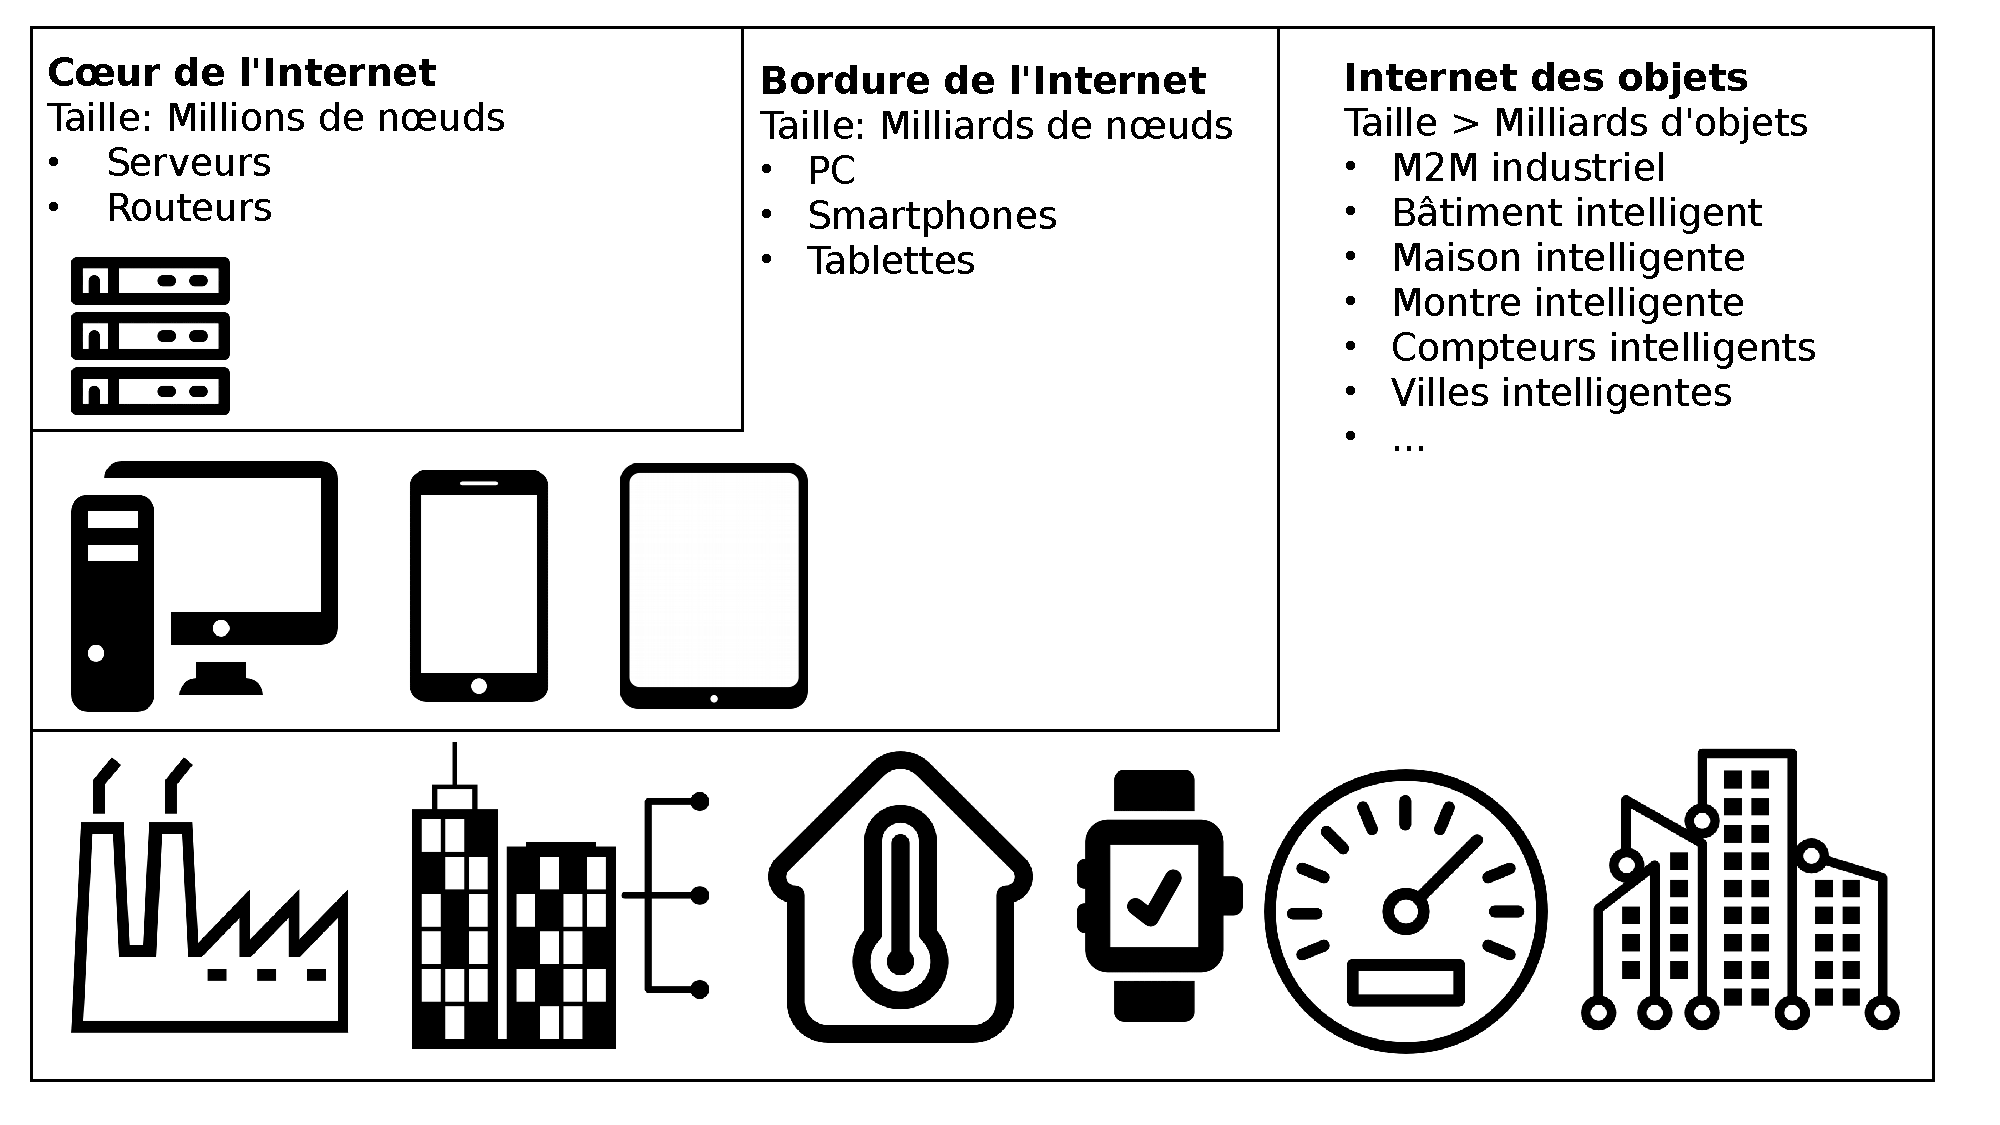
\includegraphics[width=.8\linewidth]{img/iot_vision.pdf}
	\caption{Internet des objets (IoT)}
	\label{intro:iot_vision}
\end{figure}

Internet s'est développé au cours des dernières décennies, partant d'un petit réseau académique pour devenir ubiquitaire et mondial~\cite{pujolle2014reseaux}.
La conception de ce réseau avait pour hypothèses de départ les contraintes technologiques de l'époque: des ordinateurs, toujours connectés, alimentés en énergie en permanence et disposant d'assez de capacité pour gérer le trafic réseau reçu.
L'augmentation croissante du nombre d'appareils connectés comme des ordinateurs, tablettes ou smartphones est venue s'ajouter autour des réseaux de cœur pour l'étendre et proposer de nombreux usages plus mobiles et orientés vers les utilisateurs finaux apportant services et fonctionnalités~\cite{falaki2010diversity}.

L'Internet des objets (appelé \ac{IoT} en anglais) se construit autour des réseaux préexistants montrés sur la Figure~\ref{intro:iot_vision} et vient ajouter à des objets existants des fonctionnalités de connectivité à l'Internet.
L'objectif de l'\ac{IoT} consiste à ajouter une connectivité à Internet pour un coût négligeable à des objets afin de permettre l'émergence de nouveaux services et de simplifier leur utilisation.
Cette tendance est rendue possible par la réduction constante des besoins énergétiques, de la taille, du prix et du poids des processeurs et des capteurs qui a permis d'ajouter une connectivité sans fil à un grand nombre d'appareils~\cite{koomey2011implications}.
Le nombre de machines et leur versatilité sont en pleine croissance~\cite{gubbi2013internet} de même que les marchés pour ces appareils aussi bien dans le secteur privé que grand public.
Les domaines d'applications étant vastes il s'en suit que les applications proposées seront très diversifiées et toucheront l'ensemble de la société.

Pour fonctionner, l'\ac{IoT} repose sur des capteurs envoyant des informations sur leur environnement en temps réel vers des services à valeur ajoutée que les utilisateurs finaux consultent.
Certains de ces capteurs seront intégrés dans des systèmes embarqués devant fonctionner de manière fiable sur de grandes périodes, mais avec des ressources matérielles faibles et des batteries limitées.
Afin d'augmenter leur couverture réseau, ces systèmes sont connectés les uns aux autres pour former des réseaux maillés.
À l'interface de ces réseaux maillés et des réseaux usuels se trouve une passerelle dont l'objectif est de masquer l’hétérogénéité de ces nœuds et leurs contraintes spécifiques tout en leur offrant une connectivité native au reste du réseau.

L'objectif de cette thèse est d'étudier les fonctionnalités que l'interface entre un réseau de capteurs et un réseau conventionnel peut offrir afin d'améliorer les performances et la fiabilité de fonctionnement du réseau visé visé.


Ce chapitre introductif commence par introduire une taxonomie des machines étudiées (\ref{intro:taxonomy}) puis rappelle les enjeux et domaines d'application (\ref{intro:motivations}) et les défis apportés par cette nouvelle tendance (\ref{intro:challenges}).
Les contributions de cette thèse (\ref{intro:contributions}) et le plan (\ref{intro:thesis_outline}) seront ensuite présentés.

\section{Taxonomie des machines en \ac{IoT}}
\label{intro:taxonomy}

\begin{figure}[ht]
  \centering
  \begin{tikzpicture}

  % définition des styles
  \tikzstyle{visible}=[draw, fill=blue!50]
  \tikzstyle{hidden}=[ draw, fill=gray!20]
  \tikzstyle{router}=[circle, draw, fill=orange!50,text=black]
  \tikzstyle{child}=[circle, draw, fill=yellow!50,text=black]
  \tikzstyle{root}=[circle, draw, fill=red!50,text=black]

  

  % Réseau contraint
  \node[root] (LBR) at (-4, 0) {};
  \node[router] (2) at (-5, 1) {};
  \node[child] (3) at (-5, -1) {};
  \node[child] (4) at (-6, 2) {};
  \node[child] (5) at (-6, 0) {};

% les nœuds
  \node[draw, right=of LBR] (gw) {Passerelle};


  % \node[cloud, cloud puffs = 10, minimum width = 4cm, draw, fill = gray!10] (cloud) at (5,0) {Réseau local};
  \node[draw, cloud, cloud puffs = 10, minimum width = 3cm, draw, fill = gray!10, right=of gw] (cloud) {Réseau};
  \node[draw, right=of cloud,] (service) {Services};
  \node[draw, right=of service] (users) {Utilisateurs};  


 \node [fit=(LBR) (2) (3) (4) (5), rounded corners, draw=black!50] (lln) {};
 \node [below=.3 cm of lln] {LLN (Nœuds capteurs)};

\path

  % Réseau contraint
  (gw.west) edge[<->, very thick]  (LBR) 
  % (gw.west) edge[->, thick, bend right=20]  (LBR) 
  (LBR) edge[<->] (2)
  (LBR) edge[<->] (3)
  (2) edge[<->] (4)
  (2) edge[<->] (5)

  % Réseau conventionnel
  (gw.east) edge[<->, very thick,] (cloud.west)
  (cloud.east) edge[<->, very thick] (service.west)
  (service.east) edge[<->, very thick] (users.west)

  ;

  \end{tikzpicture}
  
  \caption{Taxonomie des différents nœuds}
  
  \label{intro:fig:taxonomie}
\end{figure}



Un réseau de capteurs (aussi désigné sous le terme plus spécifique de \ac{LLN} en anglais) désigne un  réseau formé par des capteurs et une passerelle communiquant entre eux sur des connexions radio particulièrement bruitées~\cite{gubbi2013internet}.
Certains de ces nœuds ont un rôle de routeur interne relayant les communications des autres nœuds vers la passerelle (aussi appelé routeur de bordure) afin d'augmenter la couverture d'un réseau sans augmenter les portées de transmission.
C'est ce type de réseau qui est considéré dans cette thèse.

\subsection{Nœuds capteurs}

Afin de mesurer l'environnement et d'interagir avec lui, il est nécessaire d'avoir des capteurs et actionneurs simples, représentés à gauche sur la Figure~\ref{intro:fig:taxonomie}.
Ils sont utilisés dans des contextes variés et répondent à des besoins hétéroclites~\cite{werner2006deploying}.
Ils transmettent et reçoivent des messages courts comme une mesure d'un capteur ou l'ordre de déclenchement d'un actionneur et doivent fonctionner de manière fiable durant des périodes longues.

Les améliorations technologiques sur les composants sont généralement utilisées pour baisser les coûts de production et d'exploitation, notamment en énergie, plutôt que pour améliorer les performances~\cite{murugesan2008harnessing}, ainsi leurs capacités restent limitées.
Autrement dit, les architectures matérielles sont réduites (processeur, mémoire), la consommation énergétique doit être faible et la batterie doit tenir sur de longues périodes~\cite{werner2006deploying}.
Pour qu'ils puissent avoir une grande durée de vie avec des batteries simples (piles classiques) les nœuds se mettent en veille autant que possible pour préserver leurs réserves d'énergie.

Afin de masquer l'hétérogénéité des nœuds et des protocoles spécifiques qu'ils utilisent pour se parler, ces nœuds ont besoin de passerelles pour communiquer avec l'extérieur.

\subsection{Passerelles}

Ces passerelles (parfois aussi appelée routeur de bordure) sont en charge de concilier un écosystème d'appareils hétérogènes, de collecter les données des nœuds capteurs et d'offrir une interface vers eux.
La nature hétérogène des capteurs conduit les passerelles à supporter différents types d'interfaces (par exemple: \ac{CPL}, Bluetooth, cellulaire ou encore Wifi) et protocoles réseau.
Elles masquent ainsi la spécificité des capteurs derrière une interface présentant les ressources avec un formalisme commun.

Les passerelles sont plus performantes que les nœuds capteurs et ont un rôle de médiateur entre différentes technologies, comme montré sur la Figure~\ref{intro:fig:taxonomie} .
Du fait de leur position, les passerelles disposent de beaucoup d'informations sur les nœuds capteurs et peuvent en tirer parti entre autres pour établir et optimiser des tables de routage~\cite{rfc6550} ou découvrir les services offerts par les capteurs~\cite{cirani2014scalable}.
Ces fonctionnalités peuvent s'ajouter à d'autres fonctions (Pare-feux, supervision) et seront détaillées dans le chapitre~\ref{gw}.

\subsection{Infrastructure de services}

Bien que les passerelles assurent la connectivité vers les nœuds, l'intégration de ces données est faite au niveau de serveurs distants~\cite{anton2014machine, atzori2010internet} pour faciliter le passage à l'échelle de sources d'informations multiples.
Ces serveurs peuvent être physiquement localisés dans un même réseau (par exemple dans les scénarios domotique) ou bien chez un fournisseur de services tiers pour en simplifier l'usage (accès depuis l'extérieur, fiabilité renforcée, etc.)
Ils sont représentés à droite sur la Figure~\ref{intro:fig:taxonomie} et représentent le dernier chaînon avant l'utilisateur.
On y trouve les services à valeur ajoutée en charge de traiter, analyser et visualiser les données dans une interface destinée aux consommateurs et utilisateurs finaux.

Il devient alors possible de construire des services basés sur les données collectées en temps réel comme des bulletins météo ou des prévisions de trafic routier \cite{hart2006environmental, gubbi2013internet}.
Dans cette architecture, ces fonctions d'intégration seront au plus proche des utilisateurs finaux afin que seul les alarmes, exceptions ou notifications pertinentes soient envoyées.

\section{Enjeux \& motivations}
\label{intro:motivations}

L'objectif des \ac{LLN}s consiste à offrir en temps réel des mesures et des relevés sur un grand nombre d'objets avec plus d'aisance de déploiement que ce qu'un système filaire classique peut offrir.
Déployés à grande échelle, ces capteurs fournissent des mesures régulières et systématiques de l'environnement permettant des prises de décision plus réactives sur un système complexe.
Les \ac{LLN}s sont utilisés dans des contextes très variés~\cite{anton2014machine, atzori2010internet}.
Les sections suivantes présentent plus en détail les deux principaux champs d'application des \ac{LLN}s: l'industrie et la ville intelligente.

\subsection{Applications en milieu industriel}

Les unités de production industrielle ont besoin d'avoir un contrôle et une supervision en temps réel aussi fine que possible sur leurs chaînes de production~\cite{erol2011wireless, gungor2010opportunities}.
Ces déploiements mettent en jeu des capteurs hétérogènes et doivent rapporter en temps réel les événements de manière fiable tout en s'acclimatant à des conditions variées (température, radiation, produits chimiques).
Les canaux de communications utilisés doivent être fiables, bidirectionnels (on doit pouvoir communiquer avec une machine et elle doit pouvoir répondre sans limites), avec des délais courts et des bandes passantes suffisantes pour des messages compacts.

Les systèmes de télémétrie industriels usuels (\ac{SCADA}) proposent une solution à ce problème.
Ils fonctionnent le plus souvent en filaire et dans de grands déploiements cette solution peut être difficile ou coûteuse à mettre en place~\cite{anton2014machine}.
De plus, les interconnexions entre les différents systèmes de télémétrie, qu'elles soient physiques (câble) ou bien logicielles sont très souvent propriétaires, incompatibles avec les machines de la concurrence et aux fonctionnalités limitées et peu évolutives.

Les \ac{LLN}s utilisent des protocoles interopérables et des standards ouverts entre tous les équipements de différents constructeurs ce qui permet de disposer d'une interopérabilité entre des systèmes très hétérogènes~\cite{shelby20116lowpan, walter2009implementing}.
Afin de réduire les coûts d'interopérabilité, on assiste désormais à la croissance des communications \ac{M2M} reposant sur des standards réseau compatibles avec ceux utilisés sur Internet et proposant une normalisation des interfaces applicatives.

\subsubsection{Agriculture et élevage intelligent}

Les exploitations agricoles sont en croissance du point de vue de leur superficie et de leurs productions, elles adoptent de plus en plus des méthodes de production venues du monde industriel~\cite{ruiz2009review}.
Les besoins sont nombreux: surveiller en temps réel l'état des plantations, l’irrigation, la présence de pesticide ou de produits chimiques, l'acidité des sols et des conditions météorologiques~\cite{wark2007transforming}.
Pour ces besoins, il est nécessaire de disposer de méthodes de relevés fiables de l'environnement en temps réel permettant de prendre des décisions de manière automatisée à grande échelle.
Les \ac{LLN}s offrent toutes ces possibilités et permettant par exemple de surveiller l'état de santé d'un animal s'assurer que son état et son environnement sont conformes avec les normes en vigueur et s'assurer de sa traçabilité ainsi que de sa localisation, ce qui rend les contrôles sanitaires plus rapides, fiables et systématiques sur de grandes échelles cela afin d'éviter les intoxications alimentaires~\cite{wang2006wireless}.

\subsubsection{Gestion de bâtiment - Domotique}

La domotique et la gestion de bâtiment sont des secteurs en pleine expansion~\cite{martocci2010building, ehlers1996engery}.
Le but est d'obtenir au sein d'un bâtiment un système pouvant superviser l'état de l'immeuble sur différents critères comme le chauffage, l'air conditionné, la ventilation et l'allumage des pièces, la fermeture des portes ou la détection de cambriolage~\cite{mainwaring2002wireless}.
Le faible coût et la facilité de déploiement des \ac{LLN} permettent de les installer rapidement afin d'améliorer le confort et le contrôle à distance d'un grand bâtiment ou d'une habitation.
Une fois ce contrôle disponible, il est possible de contrôler le chauffage de manière beaucoup plus automatisée sans l'intervention d'un technicien sur le site et de contrôler plus finement la dépense énergétique pour chauffer un bâtiment ce qui peut conduire à des économies importantes~\cite{egan2005emergence}.

\subsection{Applications pour les villes intelligentes}

Les villes deviennent de plus en plus peuplées et la modernisation de leur fonctionnement permet des économies et des gains de qualité de vie pour chacune d'entre elles~\cite{caragliu2011smart}.
La variété des déploiements et des autorités mises en jeu rend ce contexte différent de celui des applications industrielles où une autorité unique prend la décision d'intégrer un nouveau système à l'existant.
Le but de la ville intelligente est de permettre le déploiement de systèmes à l'échelle d'une ville ou d'un territoire afin de faciliter la vie de ses habitants~\cite{hollands2008will}.

\subsubsection{Voirie}

Les villes ont par exemple besoin de pouvoir réduire efficacement le temps passé par un automobiliste pour trouver une place de stationnement dans le but de réduire le carburant utilisé  et limiter les bouchons de circulation.
Les systèmes de Smart parking~\cite{medaglianibringing} sont un bon exemple de déploiement urbain permettant d'avoir en temps réel la disponibilité des places de parking.
Ces systèmes sont mis en place en combinant des capteurs détectant des places disponibles sur la chaussée et envoyant ces informations vers des serveurs qui les redistribuent vers des utilisateurs finaux en temps réel.
La gestion du trafic automobile et des piétons peut également être plus efficace quand le trafic est fluidifié par des feux de circulation qui s'adaptent pour le gérer au mieux~\cite{de1998optimal,faye2012distributed}.

Enfin, ces systèmes ont l'avantage de réduire les coûts de fonctionnement sur des temps courts et peuvent être justifiés facilement par la réduction des dépenses publiques et la qualité de vie améliorée pour les habitants de la ville~\cite{song2014high, lee2013integrated}.

\subsubsection{Sécurité et Urgences}

La surveillance d'infrastructure comme des voies de chemin de fer, des frontières ou bien des convois sont nécessaires afin d'assurer une sûreté de fonctionnement pour les usagers et les biens.
Dans ce genre de situation, les systèmes doivent résister à de nombreuses attaques ou altérations de leur environnement tout en étant capables de répondre en temps réel en cas d'attaque et d'être fiables tout au long du déploiement.
Des systèmes utilisant des \ac{LLN}s sont mis en œuvre dans des cas de protection et de surveillance de zone dangereuses ou sécurisées~\cite{cao2005analysis}.
Elles permettent la rapidité de déploiement sans fil, la mobilité et la détection en temps réel à moindre coût.
Ces approches peuvent être couplées avec celle des villes intelligentes dans le cas de surveillances des ponts, des routes ou de grandes structures par leurs vibrations~\cite{kim2007health} afin de pouvoir altérer le trafic quand une partie de la route n'est pas sure.
En outre, la surveillance systématique des infrastructures permet de détecter des problèmes plus rapidement et efficacement.
Le déploiement des \ac{LLN}s permet d'avoir des relevés en temps réel de ces installations.
Couplé à des actionneurs, il est possible d'effectuer certaines tâches de maintenance à distance et automatiquement et donc d'éviter de solliciter un technicien.

\subsubsection{Environnements intelligents}

Détecter un risque environnemental est une nécessité pour protéger efficacement les populations et l'environnement.
Afin de surveiller en temps réel une large zone, des moyens coûteux (photos satellites, surveillance aérienne, patrouilles) et peu réactifs sont possibles, mais ne sont pas utilisables par les autorités chargées de cette surveillance pour des raisons de coûts ou de logistique.
Les \ac{LLN}s peuvent permettre un suivi en temps réel sur des zones géographiques larges et à moindre coût afin de permettre aux autorités d'intervenir rapidement quand une alerte est déclenchée.
Des déploiements ont déjà été réalisés afin de prévenir des feux de forêt~\cite{yu2005real}, des avalanches et glissements de terrain~\cite{terzis2006slip, alippi2007adaptive}, de permettre la détection des risques sismiques et volcaniques~\cite{werner2006deploying} ou bien la supervision de la qualité de l'eau et de l'air dans des terrains industriels ou contaminés~\cite{khedo2010wireless, o2007smartcoast}.
Les scénarios de surveillance de l'eau~\cite{xiao2010smart}, d'une rivière ou nappe phréatique sont particulièrement pertinent dans le cas de ville ou de zone géographique où l'eau est rare~\cite{kerkez2012design}.

\section{Défis introduits par les \ac{LLN}s}
\label{intro:challenges}

Les \ac{LLN}s sont des réseaux composés de systèmes embarqués caractérisés par une faible consommation énergétique, l'interconnexion native avec Internet via leur passerelle et des ressources limitées sur chaque nœud.
Les systèmes embarqués sont devenus, avec la croissance des smartphones, les appareils majoritaires en nombre sur Internet et cette croissance se maintient dans beaucoup de pays~\cite{kim2007value}.
L'objectif voulu par les \ac{LLN}s est de fournir des mesures en temps réel d'un environnement afin de permettre la création de services autour de ces données mesurées.
Cependant, les \ac{LLN}s disposent de leurs propres défis techniques qui les distinguent des systèmes embarqués usuels comme les smartphones et qui tiennent à leur nature même et à leurs déploiements.

La présentation de ces défis sera découpée en deux axes~: l'un portant sur les défis relatifs aux nœuds et l'autre sur ceux liés à la mise en réseau de ces mêmes nœuds.

\subsection{Défis liés aux nœuds}

Les nœuds capteurs sont des systèmes embarqués visant à fournir des mesures sur leur environnement et à exécuter des actions sur celui-ci~\cite{kopetz2011real}.
Ces nœuds sont composés de capteurs, d'actionneurs et fonctionnent grâce à un microcontrôleur ou bien avec un microprocesseur sur lequel s’exécute un système d'exploitation spécifique~\cite{dunkels2004contiki}.
Ces composants qu'ils soient matériels ou logiciels consomment aussi peu de ressources que possible, visent à être aussi fiables que possible, et cela pour un faible coût de production.
Contrairement à d'autres systèmes embarqués comme des smartphones, ils ne cherchent pas à être des systèmes universels ni à devenir plus performants.
Les évolutions technologiques visent à réduire leur coût et améliorer leur efficacité énergétique~\cite{koomey2011implications}.
En plus de ces contraintes spécifiques, d'autres défis viennent s'ajouter lorsque ces capteurs sont déployés dans le contexte spécifique des \ac{LLN}s.

\subsubsection{Hétérogénéité technologique et fonctionnelle}

%Pourquoi c'est important
Le grand nombre de constructeurs impliqués dans les \ac{LLN}s et la multitude des domaines d'applications a conduit à l'émergence de plusieurs standards~\cite{bandyopadhyay2011internet}.
Orchestrer un écosystème hétérogène tant en terme de domaines d'applications que de choix technologiques est donc un défi complexe à réaliser.

%Pourquoi c'est difficile
L'hétérogénéité se situe à plusieurs niveaux~: segments (grand public, industriel), chaînes de valeur (opérateur, fournisseur de service), délais de standardisation (time to market), taille du segment et influence géographique.
Cela fait que de nombreux standards coexistent et que des outils seront requis pour offrir des interfaces entre ces différents standards.
Des organismes nationaux et internationaux se penchent sur les questions d'interopérabilité et de standardisation~: Allseen Alliance, Industrial Internet Consortium, ETSI, Open Interconnect, Thread, IPSO Alliance, IEEE\ldots

\subsubsection{Cycle de vie}

%Pourquoi c'est important
Les fonctions d'un nœud capteur peuvent changer et nécessiter des mises à jour logicielles par exemple pour corriger des failles de sécurité ou ajouter de nouvelles fonctionnalités.
Un déploiement rapide des correctifs et des mises à jour est un facteur clé pour éviter l’obsolescence d'un objet connecté et les problèmes de sécurité qui en découlent~\cite{pathan2006security, wang2006survey}.

%Pourquoi c'est difficile
Toutefois, il peut être difficile de mettre à jour, par exemple quand le déploiement a lieu dans un terrain difficile d'accès comme un volcan ou une zone de montagne.
Des solutions de migrations, de maintenance et de déploiement d'applications à distance sont donc requises~\cite{brown2006updating, stathopoulos2003remote}.

\subsection{Défis liés au réseau}

Les nœuds capteurs disposent d'une faible capacité d'émission radio, ainsi les mettre en réseau afin qu'ils communiquent entre eux vers une passerelle permet d'améliorer la couverture du réseau tout en maintenant des portées de transmissions faibles.
Cependant la mise en réseau des \ac{LLN}s comporte des défis techniques.

\subsubsection{Pertes}

Les \ac{LLN}s utilisent généralement des bandes de fréquences libres (\ac{ISM}) pour communiquer afin d'éviter les coûts d'une licence pour une fréquence propre.
Les canaux étant communs, les liens sont bruités, instables et les pertes de paquets sont donc courantes~\cite{baccour2012radio}.
De plus, les capteurs émettent avec une faible puissance pour économiser de l'énergie ainsi ils sont particulièrement sensibles aux conditions du canal et leur signal peut être écrasé par d'autres signaux émis dans la même bande de fréquence comme du Wi-Fi.
En outre des phénomènes d’atténuation dus à la réverbération (Multipath fading) se produisent et perturbent les communications mêmes si elles sont à portée de transmission \cite{puccinelli2006multipath}.

%Pourquoi c'est important

En cas de trop fortes pertes et de conditions trop instables sur le réseau, les \ac{LLN}s peuvent adapter la topologie de routage utilisée pour communiquer plus efficacement avec la passerelle~\cite{clausen2011critical}.
Ceci peut provoquer des reconfigurations dans tout le \ac{LLN}, ainsi des mécanismes doivent être mis en place dans les protocoles pour garantir la connectivité et la fiabilité des communications entre les capteurs et la passerelle à moindre coût énergétique~\cite{6tisch}.

\subsubsection{Connexions intermittentes}

%Pourquoi c'est important
Afin d'économiser autant d'énergie et de bande passante que possible, les nœuds se mettent en sommeil régulièrement.
Durant cette période, leur consommation énergétique est significativement inférieure à la moyenne, mais le nœud est alors difficilement joignable~\cite{kellner2008towards}.
Cela entraîne l'intermittence des liaisons radio entre chaque nœud~\cite{duarte2002analysis} et implique qu'il est particulièrement difficile de savoir si un nœud est en panne, indisponible ou endormi dans le cas où ces cycles de sommeil ne sont pas déterministes.
Les appareils doivent donc gérer eux-mêmes les confirmations et la fiabilité des transmissions, car utiliser un protocole de transport classique apporterait trop de surcoûts en entêtes et retransmissions~\cite{rfc7252}.
Ainsi des protocoles sans sessions et des architectures robustes aux déconnexions sont privilégiés afin de transmettre des messages dans le \ac{LLN}.

%Pourquoi c'est difficile
% Dans le cas où les cycles d'endormissements sont gérés par une autorité centrale, il est nécessaire d'introduire une signalisation supplémentaire afin de gérer les cycles d'activité et d'utilisation du canal~\cite{6tisch}.
% Si chaque noeud gère son propre cycle d'endormissement indépendament des autres noeuds, les sources doivent émettre les messages plusieurs fois pour qu'il puisse être eventuellement reçu~\cite{dunkels11contikimac}.
% Enfin quelque soit le mécanisme d'endormissement utilisé, il existe des attaques au déni de sommeil empêchent les nœuds de dormir et use leurs ressources déjà limitées pour rendre à terme le réseau indisponible~\cite{raymond2008denial}.

\subsubsection{Besoin de protocoles optimisés}

%Pourquoi c'est important
Dans les déploiements classiques des \ac{LLN}s, les quantités de données échangées sont très réduites et intermittentes afin de préserver l'énergie~\cite{tan2010future}.
Cela requiert d'utiliser des protocoles spécifiques (compact, sans maintien d'état, avec des entêtes compressés) qui réduisent leur impact autant que faire se peut~\cite{Winter2012,shelby20116lowpan,rfc6690}.

%Pourquoi c'est difficile
Les protocoles classiques utilisés dans l'état de l'art pour faire fonctionner l'Internet ont été conçus pour des appareils étant toujours allumés, générant un trafic important et en croissance.
En outre, utiliser les protocoles classiques occuperait une quantité importante de la bande passante et engendrerait donc un surcoût non négligeable de consommation d'énergie.
L'émergence de ces protocoles justifie l'apparition d'une couche applicative d'interopérabilité afin d'orchestrer les différents nœuds sans se focaliser sur leurs spécificités~\cite{van2008achieving}.

\subsubsection{Écoute passive en zone dense}

%Pourquoi c'est important
De nombreux protocoles d'accès utilisés dans les \ac{LLN}s sont asynchrones afin d'éviter de mettre en place une signalisation régulière coûteuse en énergie et en bande passante sur chaque nœud.
Lorsqu'un nœud reçoit un signal asynchrone, il doit le décoder et l'analyser afin de décider si cette transmission lui est destinée et si une tâche doit être accomplie.
Ce décodage systématique a un coût élevé dans des environnements denses~\cite{langendoen2008medium}.

%Pourquoi c'est difficile
%Eventuels renvois(Etat de l'art/section de la thèse)

Ainsi pour des déploiements denses avec un grand nombre de nœuds, il est indispensable d'utiliser des protocoles spécifiques permettant d'avoir aussi bien passage à l'échelle en nombre de nœuds que consommation énergétique minimale lors du décodage des trames émises~\cite{6tisch}.
Les phénomènes de capture typiques de l'écoute passive sont donc évités et l'énergie n'est utilisée que pour décoder des messages pertinents pour le nœud.

\subsubsection{Passage à l'échelle}

%Pourquoi c'est important
La croissance du nombre d'appareils connectés à Internet reste forte et l'ajout des nœuds venant des \ac{LLN}s ne fera qu'accentuer cette croissance, car la baisse continue des coûts de production conduit à des nœuds toujours plus nombreux et moins cher~\cite{tan2010future, loomis2012forecasting}.
Cela pose la question du passage à l'échelle de ce type d'installation dans des réseaux qui peuvent déjà être chargés~\cite{murugesan2008harnessing,brownlee2002understanding,bandyopadhyay2011internet}.
La question du passage à l'échelle concerne à la fois la coordination des nœuds, le partage de leurs ressources et les besoins d'adressage.

Afin de répondre à un besoin croissant d'adressage, IPv6 a été introduit afin de fournir un espace d'adressage global suffisant.
L'émergence des \ac{LLN}s rend IPv6 encore plus pertinent, car il permet de disposer d'un adressage complet de tous les nœuds sur un réseau commun qu'il soit global ou privé sans utiliser de mécanisme intermédiaire coûteux comme un mécanisme de traduction d'adresse réseau (\ac{NAT}).
Cette identification unique permet de facilement fournir une communication sans intermédiaire et simplifie la gestion du réseau par un formalisme commun.
De plus, des mécanismes de compression d'IPv6 sont disponibles afin de bénéficier de l'espace d'adressage tout en limitant la taille des entêtes utilisés.

% \subsubsection{Fragmentation}

% La fragmentation arrive lorsqu'un paquet plus grand que la \ac{MTU} est transmis~\cite{shelby20116lowpan}.
% Ce type de problème peut arriver en \ieee{} où les paquets sont limités à 127 octets~\cite{ludovici2011forwarding}.
% La fragmentation peut également donner lieu à des attaques où les nœuds surchargent leur mémoire avec des paquets intermédiaires et non reconstitués~\cite{hummen20136lowpan}.

% \subsubsection{Mobilité}

% La mobilité des nœuds peut entraîner des pertes de connectivité, des reconfigurations de topologie réseau et des congestions~\cite{lee2012rpl}.
% Dans le cas des \ac{BAN}, le réseau entier peut être mobile~\cite{chen2011body} et gérer des connexions/deconnexions régulièrement.
% Des mécanismes de découvertes de voisins et de topologies peuvent permettre de gérer les cas de mobilité au sein d'un même \ac{LoWPAN}~\cite{oliveira2011routing}.

\section{Aperçu des contributions}
\label{intro:contributions}

La passerelle jour un rôle clé dans la mesure, car elle interface le \ac{LLN} avec le reste du réseau.
Elle sert de médiateur et traite donc la problématique de l'interopérabilité des nœuds et des différentes contraintes des capteurs.
Sa position dans le réseau lui permet en outre d'avoir une vue précise du \ac{LLN} et des informations qui y rentrent et en sortent.

Le but de cette thèse est d'exposer comment des fonctionnalités peuvent être ajoutées à l'interface d'un \ac{LLN} et du reste du réseau pour améliorer l'utilisation des ressources et la connaissance de l'état du \ac{LLN}.
Les contributions proposées dans cette thèse ont pour objectif d'améliorer les performances et la fiabilité d'un \ac{LLN}.


\subsection{Mesure implicite de la consommation énergétique d'un \ac{LLN}}

% \subsubsection{Description du problème}

Pour s'assurer que le fonctionnement d'une application est correct, un administrateur a besoin de connaître l'état des nœuds du \ac{LLN} dont dépend son application.
Préserver l'énergie consommée est un problème clé pour ce type de réseau.
Il parait donc naturel de mettre à disposition des administrateurs un moyen peu consommateur d'énergie leur permettant d'estimer l'état de leur réseau, d'obtenir une durée de vie estimée et connaître les nœuds les plus sollicités dans une topologie multi sauts.

% \subsubsection{Limites de l'état de l'art}

Mesurer explicitement ces informations n'est pas toujours possible et même quand c'est le cas, il est coûteux de le demander à chaque nœud dans un réseau de grande taille.
Ainsi des approches induisant un minimum de transmissions de données peuvent aider à obtenir une cartographie de la consommation énergétique et de l'utilisation de la radio à moindre coût.

% \subsubsection{Contributions}

Le chapitre~\ref{supervision} montre comment l'observation du trafic routé passant par la passerelle permet d'inférer l'utilisation de la radio, et, dans une certaine mesure, la consommation énergétique.
Les limites de cette approche seront également décrites et une correction des biais sera proposée lorsque la supervision active est possible.

\subsection{Optimisation des ressources du \ac{LLN} avec un cache intelligent}

% \subsubsection{Description du problème}
La passerelle offre une interface vers le \ac{LLN} et reçoit les requêtes applicatives qui lui sont destinées.
Le traitement d'une requête par le \ac{LLN} est lent, car les nœuds sont peu performants.
De plus chaque requête consomme de l'énergie qui est une ressource limitée.
Ainsi la passerelle a pour objectif de solliciter le \ac{LLN} aussi peu que possible tout en répondant de manière fiable aux requêtes.

% \subsubsection{Limites de l'état de l'art}

Une stratégie usuelle pour accélérer les réponses et économiser de l'énergie consiste à maintenir dans un cache au niveau de la passerelle la réponse à une requête donnée pendant un temps de validité précis.
Ainsi si la passerelle dispose d'une réponse encore valide pour une requête donnée, elle l'utilise au lieu de solliciter le \ac{LLN}.
Déterminer le temps de validité d'une réponse pour chaque ressource doit tenir compte de multiples paramètres et la littérature n'offre pas de méthode explicite pour déterminer des temps de validité efficace pour une configuration donnée.

% \subsubsection{Contributions}

Le chapitre~\ref{cache} propose de déterminer les temps de validité pour réguler le trafic entrant vers les nœuds du \ac{LLN} en fonction de la durée de vie des nœuds visée par l'administrateur et fraîcheur des réponses attendues.
Les objectifs étant antagonistes, il est nécessaire de procéder à un arbitrage afin de trouver un compromis entre différentes solutions.
Une modélisation donnée sous la forme d'une optimisation multi-objectifs permettra de fournir un ensemble de solutions admissibles optimales.

\subsection{Expériences automatisées et reproductibles pour \ac{LLN}s}

% \subsubsection{Description du problème}

Effectuer une expérience avec des \ac{LLN}s met en jeu de nombreux logiciels et des procédures qui sont longues et fastidieuses lorsqu'elles sont réalisées manuellement.
Cela rend une expérience difficile à reproduire surtout si elle n'est pas ré-effectuée par la ou les mêmes personnes.
Lorsque de nombreuses étapes sont nécessaires pour obtenir un résultat, documenter et automatiser l'expérience en question autant que possible devient crucial afin qu'elle puisse être reproduite et validée par la communauté scientifique et de s'assurer de leur véracité efficacement.

% \subsubsection{Limites de l'état de l'art}

Les bancs de test (appelés testbeds en anglais) prévus pour les \ac{LLN}s fournissent de nombreux outils dédiés au lancement d'expériences et à la collecte de résultats~\cite{buchert2015survey,fleury2015fit}.
Cependant il n'existe pas de solution complète pour lancer, récupérer et exploiter les données issues d'expériences et de simulations dans un seul outil cohérent et intégré.
En outre, l'un des écueils à éviter lors de la conception de tels outils est de définir une architecture trop spécialisée et donc inutilisable dans d'autres contextes ce qui limiterait d'emblée son impact.

% \subsubsection{Contributions}

Le chapitre~\ref{makesense} propose un framework d'organisation d'expérience permettant de documenter, d'exécuter et d'analyser l'ensemble d'une expérience sur \ac{LLN}.
Fonctionnant à la fois en simulation et sur nœuds réels, Makesense permet d'obtenir un framework d'expériences reproductibles.
Ce chapitre consacré à Makesense illustrera son fonctionnement au travers d'une expérience typique.
Il présente entre outre les étapes clés d'une expérience et montre que les choix technologiques ne requièrent pas une implémentation spécifique, mais utilise au contraire des outils classiques et largement utilisés par la communauté scientifique.
Enfin, un mécanisme d'intégration continue automatisera l'expérience et apportera ainsi la preuve de sa reproductibilité.

\subsection{Collaborations extérieures faites durant la thèse}

Un aperçu des collaborations extérieures effectuées au long de cette thèse avec des chercheurs extérieurs à notre équipe de recherche est disponible en annexe~\ref{collaborations}.

\section{Plan du manuscrit}
\label{intro:thesis_outline}

Les contributions de cette thèse exposent différentes fonctionnalités et améliorations que la passerelle peut offrir afin d'améliorer les performances et la fiabilité de ces réseaux.

Le chapitre~\ref{gw} introduit plus en détail les \ac{LLN}s.
Il présente les hypothèses de travail et les choix faits dans cette thèse pour interfacer un \ac{LLN} avec d'autres réseaux et les confronte avec ceux couramment trouvés dans la littérature.

Le chapitre~\ref{supervision} montre comment la mesure des temps d'utilisation de la radio dans un \ac{LLN} permet de prévoir la consommation énergétique implicitement.

Le chapitre~\ref{cache} expose comment l'utilisation d'un cache applicatif peut être adapté pour optimiser l'utilisation des ressources d'un \ac{LLN} en modifiant les temps de validité des réponses des requêtes qu'il reçoit.

Le chapitre~\ref{makesense} présente Makesense le framework d'expérimentation utilisé ultérieurement dans les chapitres~\ref{cache} et \ref{supervision} pour documenter, reproduire et partager les expériences effectuées sur les \ac{LLN}s.

Enfin, le chapitre~\ref{conclusion} conclue cette thèse et ouvre sur des prolongements possibles.

% L'annexe~\ref{contikimac} présentera une modélisation de ContikiMAC,
% Des extraits de code utilisés par Makesense seront présentés dans l'annexe~\ref{code} et 
L'annexe~\ref{collaborations} présentera les collaborations extérieures faites pendant cette thèse et présentera les publications obtenues.

% !TEX root = ../main.tex
% !TeX spellcheck = fr_FR

\chapter{Caractéristiques d'une passerelle pour \ac{LLN}}
\label{gw}

\epigraph{We build too many walls and not enough bridges.}{Isaac Newton}

\minitoc

Ce chapitre considère les différentes solutions techniques existantes pouvant être adoptées notamment à la passerelle pour déployer un \ac{LLN}.
Les choix techniques effectués dans cette thèse seront justifiés en prenant en compte les fonctionnalités souhaitées.

La section~\ref{gw:interop} couvre les contraintes d'interopérabilité au travers d'une présentation des différentes solutions d'accès sans-fil aux nœuds et détaille comment les connecter à un réseau IP classique en leur fournissant un adressage commun.

La section~\ref{gw:routing} couvre les contraintes liées au routage dans les \ac{LLN} et motive les choix faits dans cette thèse.

La section~\ref{gw:app_layer} aborde comment des fonctionnalités d'interfaces applicatives efficaces peuvent être déployées sur la passerelle afin d'améliorer la rapidité des requêtes et faciliter leur intégration avec des services déjà existants.

La section~\ref{gw:supervision} présente les fonctionnalités de supervision déployables sur la passerelle et comment elles peuvent être appliquées pour connaître l'état des nœuds.

La section~\ref{gw:conclusion} conclut ce chapitre, récapitule les choix techniques effectués et introduit les contributions relatives à la passerelle couvertes dans les chapitres suivants.

\section{Technologie sans-fil et adressage}
\label{gw:interop}

Comme expliqué dans le chapitre~\ref{intro}, les \ac{LLN}s mettent en jeu des nœuds hétérogènes avec des architectures matérielles très variées.
Les spécificités propres à chaque nœud doivent être masquées pour les administrateurs et fournisseurs de services afin qu'ils puissent se concentrer sur le développement de service à valeur ajoutée plutôt que sur les particularités de chaque nœud.
% Il n'est pas envisageable que chaque nœud adopte un langage universel (car il n'assurerait pas de compatibilité avec de nouvelles versions du langage, et le supporter sur les nœuds déjà déployés n'est pas forcément possible en pratique).
Dans cette thèse, on considère donc que cette opération est déportée sur une passerelle qui est plus adaptée en raison de sa position d'interface et des ressources supplémentaires dont elle dispose.

D'un point de vue matériel, une passerelle est un équipement réseau disposant d'au moins une interface connectée au \ac{LLN} et d'au moins une interface connectée à un réseau classique fonctionnant par exemple avec IP.
Cette passerelle dispose de plus de ressources qu'un nœud capteur et peut rester éveillée en permanence.
Elle peut être administrée via une interface graphique comme une interface web.

\subsection{Communication vers \ac{LLN}s}
\label{gw:low_layers}

Des solutions filaires comme le \ac{PoE} permettent de fournir alimentation électrique et connectivité aux capteurs.
Cependant, ces solutions filaires peuvent être très coûteuses et difficiles à déployer, notamment dans de grandes zones ouvertes et difficiles d'accès.

Les technologies sans-fil apportent une solution efficace et pratique de connectivité pour l'\ac{IoT} en utilisant pour leurs transmissions des bandes de fréquences \ac{ISM} qui présentent l'avantage d'être libres de droits et ne nécessitent donc pas de licence.
Les \ac{LLN}s s'appuient sur ces technologies sans-fil afin de simplifier les déploiements et réduire leurs coûts opérationnels.

Plusieurs solutions sont disponibles~\cite{wifiCritic}, chacune d'elle offrant un compromis entre la bande passante, la portée et la consommation énergétique des équipements mis en jeu.
On peut distinguer deux grandes catégories de technologies sans-fil~: d'une part celle offrant un accès de longue portée (plusieurs kilomètres) et d'autre part celle offrant un accès de courte portée (moins d'un kilomètre).

\subsubsection{Accès longue portée}
\label{gw:long_range}

Les accès de type cellulaire permettent de fournir un accès Internet à un grand nombre d'appareils mobiles~\cite{kim2007value}.
Cependant, ils ne sont pas adaptés au cas des \ac{LLN}s, d'une part en raison du prix de fabrication des composants radios dont ils ont besoin, du coût de l'accès (licence, abonnement auprès d'un opérateur) et d'autre part par la consommation énergétique qu'ils induisent.
Ainsi des technologies plus adaptées aux \ac{LLN}s sont requises pour offrir des accès longues portées.

Les technologies dites \ac{LPWAN} permettent de transmettre un volume de trafic faible~\footnote{Environ 200 octets (typique) à 5000 octets (maximum) émis par jour avec une charge applicative utile de l'ordre de 12 octets} sur des distances longues~\footnote{5 à 40 kilomètres en champ libre} à un faible débit~\footnote{Débit de 0.250 à 11 kb/s en fonction de la technologie radio}~\cite{xiong2015low}.

Ces technologies offrent un jeu de compromis clair~: peu de débit, une grande portée, une bonne pénétration~\footnote{Important pour des objets situés dans des caves comme des compteurs électriques.}, un coût de composant radio faible~\footnote{Moins de 2 dollars} et qui consomme très peu d'énergie.

Cependant, ces technologies présentent plusieurs limitations.
Les stations de base lorsqu'elles émettent utilisent une puissance supérieure à celle autorisée pour les usages privés (four à micro-ondes, Wi-Fi, etc.) sur les bandes \ac{ISM}~\cite{rec200170}.
Dans ces conditions, les autorités régulatrices de l'utilisation des bandes \ac{ISM} obligent les stations de base à transmettre au plus 1 \% de leur temps~\cite{vangelista2015long}.
Ainsi, les liens descendants sont limités bien que présents car les liens des \ac{LPWAN}s sont bi-directionnels.

De plus, les bandes de fréquences \ac{ISM} utilisées étant étroites, les liens descendant et montant sont très proches.
Ainsi, les stations ne peuvent pas actuellement transmettre vers les objets tout en écoutant avec le même niveau de sensibilité les autres nœuds de leur cellule.
Donc, dans le cas où il faut fournir un service de lien descendant (par exemple pour acquitter un paquet, mettre à jour un objet, ou déclencher des actions), l'utilisation de ces technologies doit se faire dans un contexte où le nombre de stations est surdimensionné afin d'offrir une bonne qualité de service.
Par conséquent, si le nombre d'objets devient grand, il devient nécessaire de densifier le nombre de stations de base pour fournir un canal de communication satisfaisant des stations vers les objets, ce qui augmente les coûts de déploiement.

La 5G, annoncée pour l'horizon 2020, entend regrouper et intégrer ce type de technologies longue portée pour une utilisation plus efficace des bandes de fréquences qui seront alors disponibles.

En pratique, les \ac{LPWAN}s sont orientés vers des applications où les objets publient des messages sans confirmation de leur réception (par exemple: un relevé de compteur effectué quotidiennement) et reçoivent encore moins de trafic de la part des stations de base.
Ces applications principales concernent les relevés d'informations d'équipements et de télémétries journalières.

\subsubsection{Accès courte portée}
\label{gw:short_range}

Les technologies sans-fil de courte portée offrent une alternative permettant d'avoir une bande passante et un débit plus important tout en offrant une meilleure fiabilité des transmissions.
Cependant l'utilisation de ces technologies impose un nouveau jeu de compromis.

Les nœuds peuvent être loin de la passerelle qui les connecte au reste du réseau, ainsi l'utilisation de topologies de réseau maillé est nécessaire afin d'offrir une connectivité à des nœuds étant loin de la passerelle.

Les bandes \ac{ISM} sont très chargées par de multiples appareils comme les micro-ondes ou bien d'autres appareils utilisant le Wi-Fi.
Ainsi il est nécessaire pour des nœuds d'un \ac{LLN} de disposer de mécanismes pour éviter d'avoir leurs signaux écrasés par d'autres stations émettant avec des puissances plus fortes.

D'autre part, les signaux peuvent suivre plusieurs chemins entre deux nœuds en raison des réflexions causées par l’environnement.
Ainsi un même signal peut arriver avec des amplitudes différentes et des phases différentes pouvant causer des interférences et des pertes (appelé en anglais ``multipath-fading'').
Ces conditions sont très instables et dépendent de l'utilisation d'une fréquence donnée, dans un environnement donné, à un temps donné.

Les technologies sans-fil de portée courte sont nombreuses, et seules les plus représentatives seront abordées dans les paragraphes suivants.

\paragraph{Wi-Fi}

Le Wi-Fi facilite l'utilisation d'Internet sur un grand nombre de périphériques mobiles en proposant un accès natif à un réseau IP avec des débits importants~\cite{lee2010mobile}.
Il peut fournir des topologie maillée en fonctionnant de manière ad-hoc ou bien des topologie en étoile avec un point d'accès en mode infrastructure.

Le mode la plus économe en énergie du Wi-Fi nommée \ac{PSM} permet de former un réseau entre un point d'accès et des stations à portée radio consommant peu d'énergie~\cite{anastasi2008802,tozlu2011feasibility}.
Cependant ce mode de fonctionnement impose d'utiliser le Wi-Fi en mode infrastructure avec une topologie en étoile ce qui limite la portée du réseau.

D'autre part, Wi-Fi n'est pas la technologie la plus compétitive pour les \ac{LLN} car une puce Wi-Fi est coûteuse à fabriquer et offre un débit souvent surdimensionné par rapport aux besoins des nœuds~\cite{wifiCritic}.
Ainsi, de nouvelles technologies sans-fil ont donc été conçues afin de transporter des messages à des débits plus modestes tout en consommant moins d'énergie et en restant sur les bandes \ac{ISM}.

\paragraph{Z-wave}

Z-wave permet de connecter des objets dans une topologie maillée principalement dans le secteur domotique.
Cette technologie permet d'avoir des communications fiables, avec une faible latence et un débit maximal de 100 kb/s.

Son attrait se trouve dans sa large diffusion dans le secteur de la domotique avec une large gamme de produits compatibles entre eux~\cite{zwaveCritic}.

Cependant Z-wave ne permet pas de passer simplement à l'échelle~\footnote{Limitation à 4 routeurs intermédiaires pour un réseau maillé, pas plus de 232 nœuds par réseau.} sur des scénarios avec un grand nombre de nœuds comme un bâtiment entier, une ville ou un centre commercial qui sont des cas d'utilisation importants des \ac{LLN}s~\cite{zwaveCritic}.

\paragraph{\ac{BLE}}

\ac{BLE} est une spécification complète de l'ensemble de la pile protocolaire des couches basses jusqu'à l'applicatif visant les \ac{PAN} et qui permet de connecter des objets dans une topologie en étoile sur des portées d'une dizaine de mètres.

Typiquement utilisée pour des appareils personnels (montre et bracelet connectés, accessoires de sport), cette spécification dispose de beaucoup d'atouts: un débit important (1 Mb/s) permettant de passer peu de temps à émettre, des entêtes réduits, une grande efficacité spectrale et un schéma de saut de fréquence pour éviter les canaux chargés typiques des bandes \ac{ISM}.

Cependant les portées de transmissions sont encore trop limitées et le support des réseaux maillés avec cette technologie n'est pas encore standardisé~\cite{bleCritic}.

\paragraph{\ieee{}}

\ieee{} permet de connecter des objets disposant de ressources limitées entre eux par une topologie étoilée, maillée ou arborescente sur des portées de 10 à 50 mètres avec des débits de 250kb/s.
\ieee{} est utilisée par plusieurs normes~\footnote{Zigbee~\cite{alliance2006zigbee, zigbeeCritic}, Wireless HART~\cite{lennvall2008comparison}, EnOcean~\cite{ploennigs2010performance}, \ac{6LoWPAN}~\cite{shelby20116lowpan} et plus récemment Thread~\cite{threadCritic}}.
Ainsi, ces normes permettent de disposer d'une large littérature sur ses performances et son fonctionnement.
% \ieee{} permet des communications bidirectionnelles plus flexibles avec des débits plus élevés contrairement à ce que propose les accès~\ac{LPWAN} ce qui est pertinent dans des cas où des besoins de bande passante plus élevés sont souhaitables pour envoyer une photo de surveillance par exemple.
En outre, sa consommation énergétique est faible de même que le coût moyen de ses composants radios physiques~\cite{vilajosana2015openmote}.

De plus, des techniques basées sur des sauts de fréquences sont intégrées dans les spécifications les plus récentes de \ieee{} et permettent d'augmenter sa fiabilité et de mitiger les problèmes dus au multi-path fading~\cite{6tisch}.

\paragraph{Conclusion intermédiaire}

\begin{table*}[t]
\centering
\begin{tabular}{|l|c|c|c|c|c|}
\hline
Protocole & Saut de fréquence & Débit & Topologie & Pile complète \\
\hline
LPWAN & Non & 0.250 à 11 kb/s & Étoile & Non \\
\hline
Wi-Fi (PSM) & Non & 11 Mb/s & Étoile, Maillé & Non \\
\hline
Z-wave & Non & 9.6, 40, 100 kb/s & Étoile, Maillé &  Oui \\
\hline
\ac{BLE} & Oui & 1 Mb/s & Étoile & Oui \\
\hline
\ieee{} & Possible & 250 kb/s & Étoile, Maillé & Non \\
\hline
\end{tabular}
\caption{Récapitulatif des protocoles sans-fil}

\label{gw:table:protocol_recap}
\end{table*}

Le tableau~\ref{gw:table:protocol_recap} offre un récapitulatif des technologies sans-fil considérées.
Après analyse des différentes solutions possibles, \ieee{} est le protocole qui apparaît comme le plus adapté pour construire des réseaux maillés permettant de pallier efficacement la faible portée des nœuds en augmentant la couverture et cela sans limites de nœuds.

Pour cette raison, le travail effectué dans cette thèse s'appuie exclusivement sur \ieee{}.

\subsection{Plan d'adressages dans un \ac{LLN}}
\label{gw:ip}

D'un point de vue fonctionnel, dans un réseau maillé, on distingue les hôtes simples représentés par un H sur la Figure~\ref{gw:fig:arch_6lowpan} et les routeurs représentés par un R.
Les hôtes envoient et reçoivent des messages, mais n'en transfèrent pas pour le compte d'autres nœuds.
Les routeurs font suivre des paquets entre leur origine et leur destination.
Il est à noter qu'un routeur peut également recevoir et envoyer des messages et assurer les deux fonctions (routeur et hôte).

Au vu de cette répartition des rôles dans un \ac{LLN}, il y a essentiellement trois types d'architectures possibles représentées sur la Figure~\ref{gw:fig:arch_6lowpan}.

La plus simple consiste en un \ac{LLN} connecté de manière ad hoc.
Les nœuds hôtes envoient des informations que les nœuds routeurs relaient vers leurs destinations.
Ce type de déploiement est par exemple utilisé dans des terrains sans connectivité avec un autre réseau~\cite{werner2006deploying}.

Le second type de déploiement utilise une passerelle pour assurer le rôle de routeur de bordure entre le \ac{LLN} et un réseau local.
Ce type de déploiement peut par exemple se retrouver dans un scénario domotique dans lequel tous les équipements communiquent vers la même passerelle.

Enfin un dernier type de déploiement étend le scénario du routeur de bordure pour prendre en charge le cas où des nœuds peuvent avoir plusieurs passerelles vers un réseau commun.
Ce type de déploiement peut être pertinent dans le cas où les nœuds capteurs sont mobiles et doivent pouvoir changer de passerelles tout en restant connectés au réseau et en ne changeant pas leur adresse.

Toutes ces architectures requièrent un adressage de chaque nœud afin de pouvoir garantir des communications en unicast qui sont importantes pour économiser de l'énergie et du débit par rapport à des communications broadcast.

\ieee{} fournit un identifiant (nommé \ac{EUI} en anglais) pour chaque nœud du \ac{LLN} qui est sous la forme d'un \ac{EUI}-64 dans sa version ``longue'' et qui est fournie par le constructeur.
Un identifiant plus compact \ac{EUI}-16 peut être construit à partir du précédent pour réduire la place occupée par ces adresses dans les entêtes.
Les protocoles basés sur \ieee{} utilisent ces identifiants pour construire un plan d'adressage et une passerelle est requise pour faire une éventuelle traduction entre l'adressage du réseau standard et celui utilisé dans un \ac{LLN}.

\begin{figure}[ht]
  \centering
  \begin{tikzpicture}

  % définition des styles
  \tikzstyle{visible}=[draw, fill=blue!50]
  \tikzstyle{hidden}=[ draw, fill=gray!20]
  \tikzstyle{router}=[circle, draw, fill=orange!50,text=black]
  \tikzstyle{child}=[circle, draw, fill=yellow!50,text=black]
  \tikzstyle{root}=[circle, draw, fill=red!50,text=black]

  % Ad-hoc
  \node[router] (1) at (-4, 0) {R};
  \node[router] (2) at (-5, 1) {R};
  \node[child] (3) at (-5, -1) {H};
  \node[child] (4) at (-6, 2) {H};
  \node[child] (5) at (-6, 0) {H};
  \node [fit=(1) (2) (3) (4) (5), rounded corners, draw=black!50] (lln) {};
  \node [below=.3 cm of lln] {Ad-hoc};

  \path

  % Réseau contraint
  (1) edge[<->] (2)
  (1) edge[<->] (3)
  (2) edge[<->] (4)
  (2) edge[<->] (5)
  ;

  % Simple
  \node[router] (11) at (-1, 0) {R};
  \node[router] (21) at (-2, 1) {R};
  \node[child] (31) at (-2, -1) {H};
  \node[child] (41) at (-3, 2) {H};
  \node[child] (51) at (-3, 0) {H};
  \node[visible, above=of 21] (simplelbr) {LBR};
  \node [fit=(11) (21) (31) (41) (51) (simplelbr), rounded corners, draw=black!50] (simple) {};
  \node [below=.3 cm of simple] {Simple};

  \path

  % Réseau contraint
  (simplelbr) edge[<->] (21)
  (11) edge[<->] (21)
  (11) edge[<->] (31)
  (21) edge[<->] (41)
  (21) edge[<->] (51)
  ;

  % Etendu
  \node[router] (111) at (2, 0) {R};
  \node[router] (211) at (1, 1) {R};
  \node[router] (711) at (3, 1) {R};
  \node[child] (311) at (1, -1) {H};
  \node[child] (611) at (3, -1) {H};
  \node[child] (411) at (0, 2) {H};
  \node[child] (511) at (0, 0) {H};
  \node[visible, above=of 211] (lbr1) {LBR};
  \node[visible, right=1.2cm of lbr1] (lbr2) {LBR};
  \node [fit=(111) (211) (311) (411) (511) (611) (lbr1) (lbr2), rounded corners, draw=black!50] (etendu) {};
  \node [below=.3 cm of etendu] {Étendu};

  \path

  (lbr1) edge[<->] (lbr2)
  (211) edge[<->] (lbr1)
  (211) edge[<->] (lbr2)
  (711) edge[<->] (lbr1)
  (711) edge[<->] (lbr2)
  (111) edge[<->] (211)
  (111) edge[<->] (311)
  (211) edge[<->] (411)
  (211) edge[<->] (511)
  (611) edge[<->] (711)
  (211) edge[<->] (711)
  (111) edge[<->] (711)
  ;

  \end{tikzpicture}

  \caption{Architecture réseau des \ac{LLN}s}
  \label{gw:fig:arch_6lowpan}
\end{figure}

\subsubsection{IPv4}
\label{gw:ipv4}

IP étant le protocole réseau le plus utilisé aujourd’hui, il est un candidat naturel pour fournir un adressage sur un \ac{LLN} qui soit interopérable avec un réseau existant.
Ainsi une solution consisterait à affecter une adresse IPv4 à chaque nœud.

Toutefois, IPv4 n'est pas pleinement satisfaisant principalement pour deux raisons.
D'une part la pénurie d'adresses IPv4~\cite{deering1998internet} ne permet pas d'assigner une IP publique à chaque nœud ce qui est dommageable dans le cas où des scénarios de connexions directes sont requis.
Une solution consisterait à utiliser des \ac{NAT}s~\footnote{Mécanisme permettant de disposer de plusieurs adresses privées derrière une seule adresse publique.} afin de pallier le manque d'adresses publiques allouées.
Cependant, des \ac{NAT}s requièrent de reconstruire des paquets et ce traitement dégraderait les performances en plus d'être complexe et d'invalider la connexion de bout en bout directe.

D'autre part, les en-têtes IPv4 sont relativement grands, ce qui signifie plus d'informations à transmettre et donc plus d'énergie à consommer pour transmettre un message.
Ceci pourrait être clairement amélioré puisqu'un en-tête IPv4 véhicule des informations qui ne sont pas pertinentes pour un \ac{LLN} (type de service, padding, etc.)~\cite{shelby20116lowpan}.

\subsubsection{IPv6}
\label{gw:ipv6}

Une solution alternative consiste à utiliser IPv6 afin de disposer d'un vaste espace d'adressage rendant l'utilisation d'un \ac{NAT} superflue et qui permettrait de généraliser les connexions de bout en bout sans intermédiaire.
Cependant l'utilisation d'IPv6 comporte des inconvénients dans le cas des \ac{LLN}s.
L'entête de taille fixe d'IPv6 (40 octets) est plus large que celle d'IPv4 (20 octets), d'autre part, IPv6 définit un \ac{MTU} \emph{minimal} de 1280 octets afin d'éviter les problèmes de fragmentation et de recomposition de paquets.
Or \ieee{} ne peut fournir au maximum qu'une trame de 127 octets, ainsi les paquets IPv6 venant de \ieee{} seraient rejetés par un routeur IPv6 implémentant ces recommandations de \ac{MTU} minimal.

Actuellement, IPv4 est encore largement déployé et donc les adressages IPv4 et IPv6 vont cohabiter plusieurs années~\cite{colitti2010evaluating}.
Si un \ac{LLN} utilise IPv6 pour son adressage et qu'il doit pouvoir recevoir des instructions envoyées depuis un réseau standard fonctionnant en IPv4 alors la passerelle doit assurer une conversion IPv4/IPv6 qui peut être effectuée par un mécanisme de traduction (teredo, 6to4, isatap, etc.)~\cite{conta1998generic}.

Pour transmettre des messages, il est nécessaire d'indiquer un protocole de transport pour les acheminer.
Le protocole de trafic le plus compact en terme d'en-têtes considéré dans le cadre des \ac{LLN}s est \ac{UDP}.
En effet, comparé à \ac{TCP}, il requiert moins d'espace dans l'en-tête du paquet (diminuant ainsi son coût en énergie) et n'utilise pas d'acquittements (limitant ainsi le nombre de messages et donc la consommation d'énergie).
Dans le cas où les messages doivent être acquittés, ils peuvent l'être avec un mécanisme ad hoc situé au niveau de la couche applicative.

\begin{figure}[ht]
	\centering
	% \begin{bytefield}[bitwidth=.3em]{127}
	\begin{bytefield}[bitwidth=.007\linewidth]{127}
		\bitheader[lsb=0]{23,23+21,23+21+40,23+21+40+8, 127} \\
		\colorbitbox{cyan}{23}{802.15.4}
		\colorbitbox{cyan}{21}{AES-CCM}
		\colorbitbox{Fuchsia}{40}{IPv6}
		\colorbitbox{orange}{8}{UDP}
		\colorbitbox{ForestGreen}{33}{{\footnotesize  DATA (33 octets)}}
		\colorbitbox{Salmon}{2}{\rotatebox{90}{\scriptsize FSC}}\\
		\colorbitbox{cyan}{23}{802.15.4}
		\colorbitbox{cyan}{21}{AES-CCM}
		\colorbitbox{Fuchsia}{40}{IPv6}
		\colorbitbox{LimeGreen}{20}{TCP}
		\colorbitbox{ForestGreen}{21}{{\footnotesize  DATA (21 octets)}}
		\colorbitbox{Salmon}{2}{\rotatebox{90}{\scriptsize FSC}}
		\end{bytefield}
	\caption{Trame 802.15.4 sur IPv6 (sans compression d'en-tête)}
	\label{gw:fig:802154}
\end{figure}

Une application directe de cette configuration est représentée sur la Figure~\ref{gw:fig:802154} qui représente une trame \ieee{} de donnée (``Data frame'' en anglais).
En \ieee{}, la taille maximale de données fournie par la couche physique (\ac{PLSDU}) est de 127 octets.
Utiliser IPv6 sans compression sur cette trame de données de 127 octets impliquerait de laisser seulement 33 octets utilisables pour des messages applicatifs puisque 25 sont pris par \ieee{}~\footnote{L'entête de sécurité représenté par AES-CCM sur la Figure~\ref{gw:fig:802154} est optionnel et peut consommer jusqu'à 21 octets}, 40 par IPv6 et 8 par \ac{UDP}; soit une efficacité de 26\%.
\ac{TCP} offre un rendement encore moins bon, car son entête prend plus de place que celle d'\ac{UDP}.
Afin d'améliorer ce rendement, il est nécessaire de procéder à une compression permettant d'empiler et d'abréger les informations contenues dans l'en-tête IPv6.
C'est ce que propose \ac{6LoWPAN}.

\subsubsection{6LoWPAN}
\label{gw:6lowpan}

\ac{6LoWPAN}~\cite{rfc4919} est une couche d'adaptation d'IPv6 à \ieee{} qui permet d'augmenter le rendement des trames.

\ac{6LoWPAN} définit entre autres, un format de trame pour la transmission des paquets, une méthode pour définir les adresses en lien local et des configurations d'adresses automatiques, la compression des entêtes et le processus de transfert de trames dans les réseaux maillés~\cite{rfc4944}.

\begin{figure}[ht]
	\centering
	% \begin{bytefield}[bitwidth=.3em]{127}
	\begin{bytefield}[bitwidth=.007\linewidth]{127}
		\bitheader[lsb=0]{23,44,44+7,44+7+4, 127} \\
		\colorbitbox{cyan}{23}{802.15.4}
		\colorbitbox{cyan}{21}{AES-CCM}
		\colorbitbox{Fuchsia}{7}{\rotatebox{90}{\scriptsize IPv6}}
		\colorbitbox{orange}{4}{\rotatebox{90}{\scriptsize UDP}}
		\colorbitbox{ForestGreen}{70}{DATA (70 octets)}
		\colorbitbox{Salmon}{2}{\rotatebox{90}{\scriptsize FSC}}\\
		\colorbitbox{cyan}{23}{802.15.4}
		\colorbitbox{cyan}{21}{AES-CCM}
		\colorbitbox{red}{5}{\rotatebox{90}{\scriptsize Frag}}
		\colorbitbox{Fuchsia}{7}{\rotatebox{90}{\scriptsize IPv6}}
		\colorbitbox{orange}{4}{\rotatebox{90}{\scriptsize UDP}}
		\colorbitbox{ForestGreen}{65}{DATA (65 octets)}
		\colorbitbox{Salmon}{2}{\rotatebox{90}{\scriptsize FSC}}
		\end{bytefield}
	\caption{Trame 802.15.4 avec entête de fragmentation et Entête IPv6 ``Header Compression''}
	\label{gw:fig:headers_6lowpan}
\end{figure}


Comme montré sur la Figure~\ref{gw:fig:headers_6lowpan}, la compression ne se fait pas au niveau du paquet tout entier car en cas de fragmentation et de perte d'un paquet il serait impossible de reconstituer le paquet original.
La compression se passe au niveau de l'entête IPv6 et de l'entête \ac{UDP} par deux mécanismes de compression~\cite{rfc4944}.

Afin de ne pas utiliser de processus complexes nécessitant de maintenir des états, les compressions sont sans états ou dépendent d'un contexte global à l'ensemble du \ac{LLN}~\cite{shelby20116lowpan}.
\ac{6LoWPAN} effectue une compression en retirant entre autres le préfixe IPv6 qui est le même au sein du réseau et en compressant les \ac{IID} qui sont basées sur l'adresse \ac{MAC} et déjà présentes dans les en-têtes \ieee{}.

Ainsi, \ac{6LoWPAN} permet de disposer de la compatibilité avec les réseaux IPv6 tout en disposant d'en-têtes compressés pour permettre de transmettre des messages applicatifs plus larges pouvant tenir dans la trame entière sans nécessiter de fragmentation.

\section{Routage}
\label{gw:routing}

Lorsqu'un \ac{LLN} utilise un réseau maillé pour communiquer (notamment en raison de la faible portée de transmission des nœuds), il est nécessaire de disposer d'un protocole de routage afin que les nœuds routeurs en charge de router les paquets puissent le faire.
Cependant les contraintes propres aux \ac{LLN}s se distinguent de celles des cas classiques de routage disponibles pour les réseaux usuels.

\subsection{Contraintes du routage dans les \ac{LLN}s}

L'objectif d'un protocole de routage pour \ac{LLN} est entre autres de minimiser la consommation d'énergie et de supporter les cycles de veille des nœuds en utilisant aussi peu de bande passante que possible.

\subsubsection{Faible empreinte sur les ressources d'un nœud}

Les routeurs utilisés dans les \ac{LLN}s sont généralement des nœuds capteurs eux-mêmes afin de simplifier les déploiements.
Ainsi, ces nœuds ne disposent généralement que d'une même interface radio pour traiter les paquets qu'ils doivent router pour le compte d'autres nœuds et leurs propres paquets.

De plus, les \ac{LLN}s mettent en jeu des nœuds fortement contraints ainsi un protocole de routage adapté doit induire aussi peu de signalisation que possible et doit nécessiter un faible espace mémoire.

En outre, le protocole de routage doit supporter les conditions imposées par les économies d'énergies (cycles de veille, bande passante limitée, \ldots).

\subsubsection{Détection des boucles}

Chaque équipement maintient dans sa table de routage quel voisin traverser pour joindre une destination.
Le protocole de routage doit maintenir ces routes qui doivent refléter la topologie courante du réseau, y compris si celle-ci est modifiée.
Dans ce genre de situation, les messages de routage permettent aux différents équipements de corriger leur table de routage.
Une telle correction, appelée convergence, peut prendre quelques (milli)secondes.
Cependant, rien ne garantit l'ordre dans lequel chaque routeur corrigera sa table de commutation, ni même que toutes les destinations seront joignables pendant que le réseau converge de nouveau.
Il arrive parfois que les paquets soient propagés de nouveau de manière incohérente et que des paquets soient propagés le long d'un cycle arbitraire sans jamais atteindre leur destination.
On parle alors de boucle de routage.

Dans un réseau classique, une boucle de routage se traduit généralement par une saturation des interfaces mises en jeu dans la boucle (puisque les paquets s'accumulent dans la boucle), ce qui induit de la gigue sur les autres paquets amenés à traverser ces interfaces.
Le \ac{TTL} permet d'éviter qu'un paquet soit indéfiniment repropagé et donc limite ce phénomène.
Toutefois, un paquet dont le \ac{TTL} expire est jeté et est perdu, ce qui force sa source à le retransmettre (sous réserve qu'elle le détecte).

Dans un réseau \ac{LLN} une boucle de routage est encore plus négative.
D'une part l'utilisation d'\ac{UDP} au lieu de \ac{TCP} fait qu'une perte sera généralement définitive.
De plus, tout paquet capturé dans une boucle de routage engendre une perte sèche d'énergie, puisque la plupart du temps le paquet ne sera pas acheminé jusqu'à sa destination.

Pour toutes ces raisons, la détection d'une boucle de routage et son élimination est critique.

\subsubsection{Routage optimisé pour les types de trafic typiques des \ac{LLN}s}

Les protocoles de routages classiques comme \ac{OSPF}~\cite{rfc5340} ou \ac{BGP}~\cite{rfc4271} qui sont utilisés dans les réseaux classiques sont agnostiques concernant la direction et l'intensité du trafic émis.
Cependant, les \ac{LLN}s sont des ``stub networks'', ils disposent de leur réseau, mais ne font pas transiter de paquets pour d'autres réseaux: un nœud ne fera du routage que pour des nœuds appartenant au même réseau.
D'autre part, dans un \ac{LLN} les profils de trafic observés peuvent être répartis entre trois types de trafic.

\paragraph{\ac{MP2P}}

La mission essentielle des nœuds capteurs consiste à envoyer des relevés vers une racine, on parle alors de trafic remontant ou de \ac{MP2P}.
Ainsi la passerelle a un rôle prépondérant pour un protocole de routage puisqu'elle offre un  point de sortie pour chaque nœud qui veut envoyer des messages vers l'extérieur.
Donc, un protocole de routage idéal pour les \ac{LLN}s doit être optimisé pour ce type de trafic où les paquets en provenance des nœuds remontent vers une passerelle.

\paragraph{\ac{P2MP}}

Les nœuds capteurs peuvent aussi recevoir des paquets en unicast de la part de la passerelle on parle alors de trafic descendant ou \ac{P2MP}.
Ce type de trafic est représentatif de l'envoi d'une requête ciblée ou bien du déploiement d'une mise à jour sur un nœud capteur donné.

\paragraph{\ac{P2P}}

Les cas de trafic \ac{P2P} doivent être supportés, car ils sont possibles par exemple pour faire une découverte de ressources locales ou effectuer une action, mais ces cas sont minoritaires et le protocole de routage idéal doit concentrer ses optimisations sur les deux premiers types de trafic.

\subsection{Taxonomie des protocoles de routage}

Le routage dans les \ac{LLN}s a été étudié en profondeur pour le groupe de travail \ac{ROLL} de l'\ac{IETF}~\cite{draft-ietf-roll-protocols-survey-07}.
Leurs travaux ont permis d'aboutir à la conclusion qu'aucun protocole de routage disponible alors (2009) ne convenait sans modifications aux spécificités des \ac{LLN}s et qu'il était donc nécessaire d'en construire un.

Une brève description des principaux types de routage et de leur compatibilité avec les \ac{LLN}s est fournie dans les sections suivantes afin de comprendre les décisions du groupe de travail \ac{ROLL}.

\subsubsection{Construction des tables}

La construction des tables dans un protocole de routage indique comment les routes vont être calculées et les informations qui seront disponibles sur chaque routeur intermédiaire.
Il existe deux principales familles de protocoles de routage: le routage à état de lien et le routage à vecteur de distance.

\paragraph{Routage à état de lien}

Dans cette approche, chaque nœud a la connaissance complète du réseau qui est un graphe.
Afin d'avoir cette connaissance, chaque nœud envoie à tout le réseau les informations à propos de ces liens et des destinations adjacentes.
Après la réception d'assez d'états de liens depuis un nombre suffisant de nœuds, chaque nœud calcule un arbre de plus court chemin depuis lui-même vers chaque destination en utilisant l'algorithme de Dijkstra~\cite{phillips1981fundamentals}.

Ce type de protocole induit une grande quantité de trafic de signalisation notamment quand la topologie des nœuds change souvent.
De plus, les nœuds ont besoin de mémoire pour stocker l'état de chaque nœud ainsi ils ne sont pas adaptés pour les \ac{LLN}s~\cite{draft-ietf-roll-protocols-survey-07}.

Il est à noter que ce type de protocole peut éventuellement être utilisé sur les routeurs de bordure qui ont suffisamment de capacité en bande passante et en mémoire pour communiquer aux éventuels autres routeurs de bordure sur le réseau, les routes disponibles vers le \ac{LLN}.

\paragraph{Routage à vecteur de distance}

Les protocoles de routage à vecteur de distance sont basés sur l'algorithme de Bellman-Ford~\cite{phillips1981fundamentals}.
Dans cette approche, chaque lien a un coût via une métrique préalablement définie.
Quand un paquet est envoyé entre deux points, le chemin de plus faible coût est choisi.
La table de routage de chaque routeur garde en mémoire les routes des destinations qu'elle connaît avec le coût de chemin associé.

Les informations de routage sont mises à jour soit de manière proactive soit réactive en fonction du protocole de routage choisi.
En raison de sa simplicité, de sa faible signalisation et de son adaptabilité, le routage à vecteur de distance est généralement appliqué aux \ac{LLN}s~\cite{rfc3561,hu2003sead,rfc6550}.

\subsubsection{Réactivité}

La réactivité d'un protocole de routage désigne comment les routes sont entretenues et découvertes au cours du temps.
Il existe deux modalités de réactivité pour le routage: le routage réactif et le routage proactif.

\paragraph{Routage réactif}

Les protocoles de routages réactifs stockent peu ou pas d'information de routage, ils découvrent dynamiquement les routes lorsqu'elles sont demandées.
Un processus de découverte de route est alors exécuté lorsqu'un routeur reçoit un paquet à router avec une destination qu'il ne connaît pas.
Ces protocoles sont notamment utilisés dans des réseaux très dynamiques, parmi ces protocoles on peut citer  \ac{AODV}~\cite{rfc3561}, avec dans le cas des \ac{LLN} le protocole de routage utilisé par Zigbee qui est dérivé d'\ac{AODV} ou plus récemment Load-ng~\cite{LoadNg-draft}.

L'avantage de cette approche est que la signalisation de routage n’apparaît que quand elle est demandée, ce qui est utile dans des cas de réseaux ad hoc où la topologie change fréquemment et où les communications sont essentiellement \ac{P2P}.
Cependant, cette approche est coûteuse dans les cas où la topologie change peu.
De plus, il est souhaitable a des fins de supervision d'avoir une vue aussi récente que possible sur la topologie du réseau.

\paragraph{Routage proactif}

Un protocole de routage proactif construit les routes nécessaires sur chaque nœud avant que les routes soient demandées.
Ainsi ces protocoles préparent proactivement toutes les routes possibles ou probables vers une destination.
La plupart des protocoles utilisés dans le routage inter-domaine ou intra-domaine utilisent un protocole proactif quand la topologie est stable.
D'autres exemples peuvent être trouvés par exemple dans des cas plus dynamiques comme \ac{OLSR}~\cite{rfc3626}.

L'avantage de cette approche est que les routes sont immédiatement disponibles quand elles sont nécessaires, cependant cette disponibilité se paye par un coût de signalisation important notamment quand la topologie change fréquemment.

\subsection{\acl{RPL}}

\ac{ROLL} a construit \ac{RPL}~\cite{rfc6550} afin de fournir un protocole de routage disposant des fonctionnalités nécessaires et adaptées aux contraintes spécifiques des \ac{LLN}s spécifiées dans leur cahier des charges~\cite{draft-ietf-roll-protocols-survey-07}.

\ac{RPL} est un protocole de routage proactif à vecteur de distance dédié aux \ac{LLN}s.
Il construit et maintient une topologie de réseau sous forme d’un graphe acyclique dirigé vers une destination (\ac{DODAG} en anglais) ayant comme racine une ou plusieurs routeur de bordure (\ac{LBR} en anglais).
Les paquets transmis par les nœuds sont transmis par les liens du \ac{DAG}.
\ac{RPL} permet le trafic \ac{MP2P} (trafic montant), \ac{P2MP} (trafic descendant) et le trafic \ac{P2P} (trafic entre nœuds).

Ce protocole de routage est standardisé, largement diffusé et est aujourd'hui considéré comme le protocole de routage standard des réseaux \ac{LLN}s.
Ainsi il est le protocole de routage de référence utilisé dans cette thèse.

\subsubsection{Structures et signalisation de routage}

\begin{figure}[ht]
	\centering
	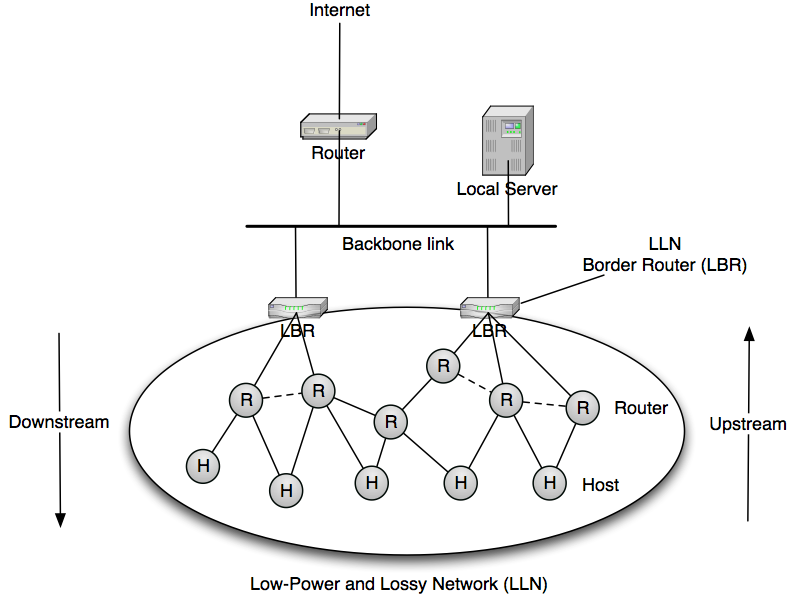
\includegraphics[width=.7\textwidth]{img/rpl.png}
	\caption{Schéma de l'architecture \ac{RPL}}
	\label{gw:fig:rpl_architecture}
\end{figure}

\ac{RPL} construit un graphe de routage entre les nœuds du \ac{LLN} et le routeur de bordure comme illustré sur la Figure~\ref{gw:fig:rpl_architecture}.
Le routage effectué par \ac{RPL} n'est valide qu'au sein du \ac{LLN} et s'arrête donc aux \ac{LBR}s.
Cette topologie est maintenue en utilisant aussi peu de messages de signalisation que possible.
Une fois construite, le protocole de routage maintient des routes montantes (\ac{MP2P} ou ``upstream'' en anglais) et descendantes (\ac{P2MP} ou ``downstream'' en anglais) et procède au routage des paquets IPv6.
% La coordination du graphe de routage ainsi que la gestion du trafic doit être faite dans un lieu centralisé.
La passerelle peut assurer cette fonctionnalité de routeur de bordure en raison de ses ressources physiques et de sa position de racine.


% \begin{figure}[tb]
% 	\centering
% 	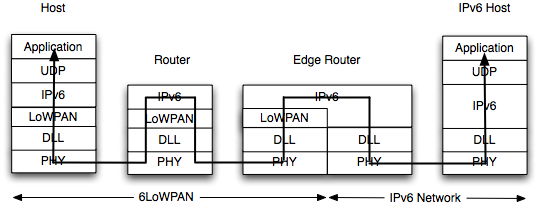
\includegraphics[width=.5\textwidth]{img/routing.png}
% 	\caption{Schéma de routage dans un \ac{LLN} à travers un routeur 6LoWPAN}
% 	\label{gw:fig:rpl_border}
% \end{figure}

Les nœuds routeurs disposant d'interfaces vers un autre lien IP sont appelés routeurs de bordure (\ac{LBR}), il peut y avoir plusieurs \ac{LBR} pour connecter un \ac{LLN} au reste d'un réseau afin d'assurer une redondance de liens de sorties souhaitable en cas de pannes.
Le rôle de \ac{LBR} est généralement accompli par la passerelle en raison des multiples interfaces de sorties dont elle dispose.

Les nœuds à l'intérieur du \ac{LLN} sont soit des routeurs soit des hôtes.
Les hôtes ne participent pas au routage et choisissent simplement un routeur par défaut, c'est par exemple le cas des nœuds fortement contraints qui ne peuvent assurer des tâches de routage pour le compte d'autres nœuds.
Les routeurs sont eux chargés de router les paquets en provenance d'hôtes ou d'autres routeurs vers leur destination finale.

\subsubsection{Construction du routage}

Pour le routage montant (\ac{MP2P}), \ac{RPL} construit un \ac{DODAG} qui démarre à partir du \ac{LBR}.
Un rang est assigné à chaque nœud (routeur ou hôte) de telle sorte que le rang augmente à mesure que l'on s'éloigne du \ac{LBR}.
Router un paquet vers le \ac{LBR} consiste à choisir un voisin avec un rang aussi faible que possible.

Le routage descendant (\ac{P2MP}) peut être implémenté de manière stockée (``storing-mode'' en anglais) ou non stockée (``non storing-mode'' en anglais) à l'échelle du \ac{DODAG} entier.
Dans le cas où le routage descendant est non stocké, un routage à la source~\cite{rfc6554} est fait quand un paquet doit être routé vers un nœud spécifique dans le \ac{LLN}.
Le routeur de bordure indique la séquence de nœuds qu'il faut traverser pour que le paquet arrive à sa destination.
Le routeur de bordure apprend ce routage en collectant les \ac{DAO}s envoyés par chaque routeur vers le \ac{LBR} et qui indique parents et enfants du routeur en question.

Lorsque le routage descendant est stocké, des tables de routages intermédiaires sont utilisées pour qu'une route partielle soit construite à chaque nœud intermédiaire qui est capable de router le paquet dans son sous-réseau, jusqu'à ce que la destination finale soit atteinte.

\subsubsection{Maintenance du routage}

Les nœuds exécutant \ac{RPL} échangent des informations de signalisation pour mettre à jour le \ac{DODAG} et ainsi mettre à jour de manière proactive la topologie de routage.
Il existe plusieurs types de messages de signalisation, celui utilisé pour construire le \ac{DODAG} est un \ac{DIO}.
Tous les nœuds dans le réseau envoient régulièrement des \ac{DIO} afin d'indiquer leur rang à leurs voisins.

Dans un \ac{LLN}, le trafic de routage et de données est limité, ainsi il est nécessaire de détecter aussi rapidement que possible les inconsistances de routage pour les corriger et éviter d'attendre un paquet de signalisation pour lancer une procédure de réparation.
Pour cela, un routeur \ac{RPL} insert une option (nommée \ac{RPL} Option~\cite{rfc6553}) dans l'entête de chaque paquet de donnée afin de détecter les éventuelles inconsistances et lancer des réparations ciblées ou globales le cas échéant.  
Par exemple, si un routeur reçoit un paquet ``descendant'' et qu'il doit l'envoyer à un nœud avec un rang plus faible ou un paquet ``montant'' et qu'il doit l'envoyer à un nœud avec un rang plus élevé alors une inconsistante est détectée et une réparation est déclenchée.

La transmission des paquets est suspendue tant que le \ac{DODAG} n'est pas remis dans un état admissible, ce qui peut occasionner des délais et des surcharges des mémoires tampons.

\paragraph{Limitation de trafic de routage (Trickle)}

\ac{RPL} utilise un mécanisme de timer adaptatif appelé  ``Trickle'' (goutte à goutte) afin de contrôler le débit d’émission des messages de signalisation (\ac{DIO}) de manière proactive.
Trickle double l’intervalle séparant deux émissions successives de messages de contrôle à chaque fois que le réseau est cohérent, et ce jusqu’à une valeur maximale.
Ainsi le trafic \ac{RPL} diminue dans le réseau lorsqu'il est stable et que la topologie change peu.
Quand une incohérence est détectée, le timer est réinitialisé à sa valeur minimale et les mécanismes de réparation sont lancés.
Un des principaux avantages de l’utilisation du timer Trickle est qu’il ne nécessite pas de code complexe et il est assez facile à mettre en œuvre dans des nœuds disposant de ressources limitées.

\section{Interface applicative}
\label{gw:app_layer}

Un protocole applicatif a pour objectif de fournir un accès aux données et services applicatifs proposés.
Parmi les exemples les plus connus d'interface applicative, on peut citer l'accès à une page web, le transfert d'un fichier ou encore l'envoi de messages électroniques~\cite{pujolle2014reseaux}.
Cependant dans le cas des \ac{LLN}s, l'utilisation principale de cette interface applicative se borne à l'envoi d'instructions courtes et le relevé d'informations sur l'environnement immédiat des nœuds.
Ainsi il est nécessaire d'utiliser des protocoles aussi optimisés que possible pour ces usages.

\subsection{Contraintes de l'interface applicative d'un \ac{LLN}}

Les \ac{LLN}s doivent s'intégrer aussi facilement que possible aux services d'ores et déjà disponibles afin de faciliter leur adoption.
Une des clés de cette intégration et d'avoir une passerelle pouvant offrir une interface commune à de nombreux nœuds.
Enfin, il est impératif que cette intégration se fasse en consommant aussi peu de ressources que possible afin de garantir la durée de vie des nœuds et le bon fonctionnement du \ac{LLN}.

\subsubsection{Interface efficace avec les services web}

Les services web sont aujourd'hui la façon la plus utilisée pour interroger des serveurs de services~\cite{alonso2004web}.
Les ressources y sont désignées par une \ac{URI} qui assure l'adressage.
L'interaction avec cette \ac{URI} utilise d'une part le protocole \ac{HTTP}, et d'autre part une architecture \ac{REST} (Architecture client-serveur, absence d'états, etc.)~\cite{richardson2008restful}.

Afin de s'intégrer aussi facilement que possible à cette architecture, il est souhaitable pour les nœuds capteurs de disposer d'une sémantique proche et de disposer d'\ac{URI} pour désigner les ressources dont ils disposent.
Ainsi lorsqu'un développeur veut utiliser une source d'information en provenance d'un capteur, celle-ci doit être aussi simple à utiliser et proche de ses habitudes que possible.

\subsubsection{Disponibilités sur plusieurs plateformes}

L'objectif de la passerelle est de masquer les spécificités de chaque nœud capteur derrière un formalisme commun afin de simplifier la tâche des développeurs.
Ainsi, une couche applicative idéale doit pouvoir être implémentée sur un large ensemble de plateformes logicielles et matérielles.

\subsubsection{Contraintes en ressources}

Les nœuds capteurs offrant des services applicatifs disposent de peu de mémoire et de ressources de calculs.
Ainsi une couche applicative efficace doit avoir des entêtes aussi limités que possible, doit imposer aussi peu d'utilisation de mémoire que possible (par exemple pour conserver un état) et doit permettre de supporter des notifications afin d'éviter de payer le coût de requête typique des protocoles synchrones et très coûteux pour les \ac{LLN}s.

\subsection{État de l'art sur les protocoles applicatifs}

Il existe de nombreux protocoles applicatifs pouvant être appliqués aux \ac{LLN}s~\cite{karagiannis2015survey}.
L'objectif de ces couches applicatives consiste à faire un compromis entre jeu de fonctionnalités, interopérabilité et consommation énergétique.

\subsubsection{Couches spécifiques à une architecture matérielle}

Les piles protocolaires totalement intégrées dans un seul standard (Zigbee~\cite{zigbeeCritic} ou \ac{BLE}~\cite{bleCritic}) proposent leur propre couche applicative standardisée qui peut être prise en charge par la passerelle.

L'avantage de cette approche est qu'elle permet de disposer d'une couche applicative certifiée et d'un fonctionnement interopérable avec tous les appareils supportant la même norme.
Cependant ces couches protocolaires ne sont disponibles que sur leur matériel propre et sont donc peu interopérables avec des nœuds hétérogènes.

\subsubsection{\ac{MQTT}}

\ac{MQTT}~\cite{hunkeler2008mqtt} est un protocole standardisé par IBM reposant sur un mécanisme de publication-souscription (``publish-subscribe'' en anglais, ou ``pub-sub'' en abrégé) utilisé pour permettre à des abonnés (par exemple des services à valeur ajoutée) de s'abonner aux mises à jour envoyées par des nœuds de manière asynchrone.

L'avantage de ce protocole est d'avoir de nombreuses implémentations, un mode de fonctionnement particulièrement adapté aux notifications et un large support via de nombreuses bibliothèques logicielles~\cite{stanford2008mqtt}.

Cependant, ce protocole repose sur \ac{TCP} qui n'est pas véritablement adapté au contexte des \ac{LLN}s car les retransmissions qu'il induit consomment bande passante et énergie.
De plus, ce protocole n'offre pas d'interface directe vers les mécanismes de services web et leur paradigme \ac{REST} sans l'utilisation d'un service tiers avec maintien d'un état~\cite{collina2012introducing}.

\subsubsection{Application directe de \ac{HTTP}}

Utiliser \ac{HTTP} directement sur les nœuds capteurs permettrait d'avoir une pile applicative classique et directement compatible avec les services web usuels.
\ac{HTTP} est largement diffusé, disponible dans de nombreux langages nativement et dispose d'une sémantique puissante via l'utilisation de \ac{REST}.

Cependant, appliquer cette approche sur les \ac{LLN}s serait coûteux car l'utilisation de \ac{HTTP} implique celle de \ac{TCP} qui n'est pas adapté pour des nœuds très contraints en raison des retransmissions.
De plus, cette approche ne supporte pas pour le moment les notifications de type ``push'' car les services web fonctionnent de manière synchrone or des communications asynchrones sont très courantes dans le cas des \ac{LLN}s par exemple pour envoyer une notification quand une condition sur l'environnement se produit.

Ainsi il est nécessaire de chercher une synthèse proposant à la fois une intégration efficace avec des services web pour faciliter l'adoption des \ac{LLN}s comme source de données pour des services web tout en utilisant un protocole applicatif peu consommateur d'énergie et un support des notifications asynchrones.

\subsection{Présentation de \ac{CoAP}}

Le groupe de travail \ac{CoRE} de l'\ac{IETF} a défini le protocole \ac{CoAP}~\cite{rfc7252} pour fournir une interface applicative générique tout en ajoutant des fonctionnalités spécifiques aux contraintes des \ac{LLN}s comme des entêtes courts et faciles à disséquer, le support de notifications asynchrones, etc.

\ac{CoAP} est le plus souvent implémenté sur un protocole de transport orienté datagramme tel que \ac{UDP} afin d'avoir des entêtes courts qui nécessitent peu de bande passante.
Ainsi il implémente un mécanisme de transport unicast pour assurer une fiabilité sans utiliser un protocole dédié comme \ac{TCP} qui peut être plus complexe à implémenter pour les nœuds capteurs et consomme plus de ressources.

\ac{CoAP} utilise une architecture \ac{REST} reposant sur des verbes usuels comme \texttt{GET}, ou \texttt{PUT} permettant ainsi de disposer d'une sémantique riche directement dans le protocole sans nécessiter le maintien d'état en mémoire pour le capteur qui serait coûteux dans le cas de mémoire contrainte.

\subsubsection{Support de notifications asynchrones}

\ac{CoAP} supporte les notifications asynchrones afin de permettre à des nœuds capteurs d'envoyer des notifications sur un modèle ``push'' à un observateur.

En pratique, il n'y a le plus souvent qu'un seul observateur afin de limiter l'utilisation des ressources d'un nœud capteur qui n'a besoin de garder qu'une seule adresse en mémoire.
Dans cette architecture, c'est le plus souvent un service qui va recueillir les notifications en provenance des nœuds capteurs et les distribuer vers les abonnés pertinents sans solliciter les nœuds capteurs.
Ce mode de fonctionnement peut être accompli par l'utilisation d'un proxy inversé (\ref{gw:reverse_proxy}).

\subsubsection{Traduction \ac{HTTP}/\ac{CoAP}}

L'un des objectifs de \ac{CoAP} est de permettre une traduction facile entre une \ac{URI} utilisée par un service web et celle qui est utilisée pour désigner la ressource d'un nœud capteur facilitant ainsi le travail des développeurs et l'intégration des \ac{LLN}s.

\ac{CoAP} n'est pas une compression naïve de \ac{HTTP} qui serait un standard complexe à implémenter et surdimensionné pour les nœuds capteurs.
La conversion entre \ac{HTTP} et \ac{CoAP} se fait sur les verbes employés (\texttt{GET}, \texttt{PUT}, etc.) et les \ac{URI} (paramètres et options compris).
La conversion est sans état et peut être faite efficacement par l'utilisation de proxys traducteurs situés entre les sources des requêtes \ac{HTTP} et les nœuds capteurs.

De plus, \ac{CoAP} supporte le traitement complet d'une \ac{URI} afin de profiter des options qu'elle contient pour répondre plus précisément à une requête (par exemple recevoir une notification si la température dépasse un seuil.)

\subsection{Traduction, proxy inversé et cache}
\label{gw:rpc}

La passerelle peut offrir une médiation applicative entre les \ac{LLN}s et les fournisseurs de services à valeur ajoutée.
Cette médiation peut être approfondie par la passerelle afin d'offrir des fonctionnalités supplémentaires ayant pour objectif d'améliorer la rapidité du traitement d'une requête et limiter la consommation énergétique des nœuds du \ac{LLN}.

\subsubsection{Traduction}
\label{gw:traduction}

Les nœuds d'un \ac{LLN} utilisent des protocoles applicatifs hétérogènes et les fournisseurs de services veulent éviter d'implémenter un support pour un grand nombre de protocoles qui serait trop coûteux.
La passerelle connaît les spécificités de chaque nœud et peut offrir des traductions de protocoles depuis des protocoles usuellement utilisés dans les services web tels qu'\ac{HTTP} vers les protocoles utilisés par les nœuds capteurs du \ac{LLN}.
Ainsi les tâches de traduction se font au plus près des nœuds capteurs et permettent de simplifier le traitement des données dans des architectures orientées service.

\subsubsection{Proxy inversé}
\label{gw:reverse_proxy}

La fonctionnalité de traduction n'est pas suffisante pour fournir un service efficace et sécurisé.
En effet, les nœuds capteurs étant contraints, ils ne peuvent recevoir qu'une quantité limitée de trafic.
De plus, s'ils sont accessibles depuis un réseau public, il est nécessaire de contrôler finement le trafic reçu afin d'éviter par exemple des attaques par déni de service ou de sommeil~\cite{wessels2001web,raymond2008denial}.

Un proxy inversé (``reverse proxy'' en anglais et désigné par \ac{RPC} dans le reste de cette thèse)~\cite{reese2008nginx} est un serveur qui se pose entre des requêtes provenant de l'extérieur et des services à protéger comme représenté sur la Figure~\ref{gw:fig:rpc}.
Le proxy inversé intercepte l'ensemble des requêtes à destination des nœuds et peut les modifier, les faire passer ou renvoyer des codes d'erreurs.

Le proxy inversé se pose en intermédiaire permettant un gain en termes de fonctionnalité  appréciable, car un administrateur peut configurer le proxy inversé pour gérer le trafic applicatif reçu par les nœuds au lieu de le configurer individuellement sur chaque nœud.
Ainsi l'administrateur du \ac{LLN} peut limiter arbitrairement les requêtes transmises aux nœuds pour limiter l'énergie qu'ils consommeraient pour y répondre.

De plus, dans le cas de notifications asynchrones, avoir un proxy inversé qui centralise les notifications est pertinent, car les nœuds capteurs ne doivent envoyer de notifications que vers une seule destination.
Lorsque la notification est arrivée sur le proxy inversé il se charge de distribuer cette notification vers les abonnés pertinents.
Ainsi la gestion d'un grand nombre d'abonnés est déportée des nœuds capteurs vers le proxy inversé et une économie d'énergie est ainsi réalisée.

\subsubsection{Cache}
\label{gw:cache}

Un cache stocke du contenu afin de l'avoir à disposition sans le redemander au reste du réseau.
Une économie de bande passante et de délai est donc réalisée à chaque fois qu'une requête est traitée par l'utilisation d'un cache au lieu d'être envoyée aux nœuds du \ac{LLN}~\cite{wessels2001web}.
À ce titre, le rapport entre le nombre de requêtes traitées par le cache sur le nombre de requêtes total (``hit rate'' en anglais)  est une métrique importante pour mesurer son efficacité.
Il est nécessaire d'avoir une politique de mise en cache, car la quantité de mémoire du cache est limitée, de plus, une information peut devenir obsolète si elle reste en cache trop longtemps.

L'utilisation d'un cache est étudiée dans les \ac{LLN}s~\cite{colitti2011rest} et notamment avec \ac{CoAP} car elle permet de faire des économies de bande passante et d'accélérer le traitement d'une requête~\cite{rfc7641}.

\subsection*{Conclusion intermédiaire}

Comme vu dans cette section, \ac{CoAP} permet d'offrir une sémantique et un jeu de fonctionnalités riches comme le support de messages asynchrones et la traduction sans état avec \ac{HTTP} tout en consommant aussi peu d'énergie que possible.

Cette intégration des notifications asynchrones est d'autant plus pertinente que les versions futures de \ac{HTTP}2 en cours de déploiement supporteront les notifications asynchrones (``push notifications'' en anglais).
Ainsi, des traductions sémantiquement complètes pourront être mises en œuvre entre \ac{CoAP} et \ac{HTTP}2.
Ces aspects sont activement étudiés aujourd'hui et accentuent la nécessité d'avoir des traductions aussi efficaces que possible autour du paradigme \ac{REST} entre les nœuds et les fournisseurs de services à valeur ajoutée, ce que \ac{CoAP} fournit.

\begin{figure}[ht]
  \centering
  \begin{tikzpicture}

  % définition des styles
  \tikzstyle{visible}=[draw, fill=blue!50]
  \tikzstyle{hidden}=[ draw, fill=gray!20]
  \tikzstyle{router}=[circle, draw, fill=orange!50,text=black]
  \tikzstyle{child}=[circle, draw, fill=yellow!50,text=black]
  \tikzstyle{root}=[circle, draw, fill=red!50,text=black]

  % les nœuds
  \node[draw] (gw) {Reverse Proxy};

  \node[draw, above= of gw] (cache) {Cache};


  % Réseau contraint
  \node[root] (1) at (-4, 0) {};
  \node[router] (2) at (-5, 1) {};
  \node[child] (3) at (-5, -1) {};
  \node[child] (4) at (-6, 2) {};
  \node[child] (5) at (-6, 0) {};

  % \node[cloud, cloud puffs = 10, minimum width = 4cm, draw, fill = gray!10] (cloud) at (5,0) {Réseau local};
  \node[draw] (cloud) at (5,0) {Réseau local};

 \node [fit=(1) (2) (3) (4) (5), rounded corners, draw=black!50] (lln) {};
 \node [below=.3 cm of lln] {LLN};

\path

  % Réseau contraint
  (gw.west) edge[<-, cyan, thick, bend left=20] node [below] {CoAP 2.05} (1)
  (gw.west) edge[->, olive, thick, bend right=20] node [above] {CoAP GET} (1)
  (1) edge[<->] (2)
  (1) edge[<->] (3)
  (2) edge[<->] (4)
  (2) edge[<->] (5)

  (cache) edge[->, very thick, cyan, bend right=20] (gw)
  (cache) edge[<-, very thick, cyan, bend left=20] (gw)

  % Réseau conventionnel
  (gw.east) edge[<-, olive, very thick, bend left=20] node [above] {GET / HTTP/1.1} (cloud.west)
  (gw.east) edge[->, cyan, very thick, bend right=20] node [below] {HTTP/1.1 200 OK} (cloud.west)
  ;

  \end{tikzpicture}

  \caption{Architecture d'un \acf{RPC}}

  \label{gw:fig:rpc}
\end{figure}

\ac{CoAP} permet de plus l'utilisation de fonctionnalités au niveau de la passerelle afin d'accélérer le traitement des requêtes et économiser de la bande passante.
Ces fonctionnalités de traductions entre \ac{HTTP} et \ac{CoAP}, de proxy inversé et de cache sont dénommées \acl{RPC} et sont résumées sur la Figure~\ref{gw:fig:rpc}.
Cette figure illustre l'exemple de l'envoi d'une requête \ac{HTTP} qui est traduite en CoAP avant d'être envoyée dans le \ac{LLN}.
Une fois la réponse \ac{CoAP} obtenue, elle est retraduite en réponse \ac{HTTP} puis mise en cache afin d'être réutilisée ultérieurement enfin la réponse \ac{HTTP} est fournie au client.

En raison de sa pertinence, \ac{CoAP} sera le protocole applicatif utilisé dans le reste de cette thèse.

\section{Supervision}
\label{gw:supervision}

La supervision désigne la surveillance continue d'un système afin de s'assurer que son fonctionnement et ses performances sont ceux attendus~\cite{ligus2012effective}.

Cette surveillance est nécessaire pour s'assurer par exemple qu'un système d'acquisition est toujours valide ou bien que ses réserves d'énergies sont suffisantes pour tenir pendant une durée donnée.
Un système de supervision peut agir en envoyant une alerte à un humain ou un autre système pour l'informer qu'un \ac{LLN} rencontre des problèmes et qu'une intervention est peut-être à prévoir.
Son objectif est alors de permettre à un administrateur d'identifier aussi rapidement que possible quel est le problème et ses causes.

Dans le cas des \ac{LLN}s, les métriques recueillies peuvent être relatives à un nœud donné par sa consommation énergétique, l'état du médium, le nombre de retransmissions, la charge moyenne, etc ou bien relatives à l'ensemble du \ac{LLN}s avec les nœuds les plus sollicités, les nœuds ayant des ressources énergétiques en dessous d'un certain seuil, la latence globale ou les erreurs applicatives, etc.

Toutes ces informations permettent de prendre des décisions motivées et justifiées sur la maintenance du réseau afin de garantir son fonctionnement.

\subsection{Fonctionnalités recherchées}

La supervision couvre plusieurs aspects fonctionnels et administratifs du fonctionnement d'un système.
Sa mise en place repose sur plusieurs objectifs fonctionnels et techniques.

\subsubsection{Suivi des équipements}

Un premier objectif de la supervision dans un \ac{LLN} consiste à connaître l'ensemble des équipements déployés, leurs fonctionnalités, depuis quand ils sont en fonctionnement.
Cette fonctionnalité d'inventaire peut être complexe à mettre en place dans le cas où les équipements changent dynamiquement et sont fortement hétérogènes.

Ce suivi des équipements est utile pour diagnostiquer des problèmes temporels pouvant survenir lors de l'ajout de matériel.
Par exemple, l'ajout d'un trop grand nombre de nœuds physiques avec une certaine configuration peut causer une perte de performance selon certaines métriques, etc.

\subsubsection{Suivi de la disponibilité}

La supervision permet d'obtenir une distinction entre un suivi dans le temps de la disponibilité matérielle et fonctionnelle d'un système qui est nécessaire pour avoir un suivi de supervision efficace.
Dans le cas d'un \ac{LLN} appliqué à un scénario de bâtiment intelligent, une supervision de disponibilité matérielle permet de savoir, par exemple, si un nœud physique donné est disponible.
Une supervision de disponibilité fonctionnelle, quant à elle, permet de savoir s'il est possible de mesurer la température sur un étage donné d'un bâtiment.

Cette distinction est essentielle afin d'avoir des alertes de supervision pertinentes et de ne solliciter des interventions humaines coûteuses uniquement pour les problèmes  critiques.

\subsubsection{Prévision}

Un autre volet important de la supervision consiste à analyser les tendances de fond d'un système afin de prévoir son fonctionnement.
Prévoir l'évolution d'une métrique permet d'éviter des accidents d'exploitations ou d'autres pannes pouvant survenir lors de l'évolution d'un \ac{LLN}.
En outre, cette prévision permet de séparer les problèmes et les alertes en fonction de leur urgence et de permettre des interventions humaines plus flexibles dans le temps.

\subsubsection{Construction de tableau de bord}

Les tableaux de bord (en anglais ``dashboards'') permettent d’agréger et de filtrer les métriques nombreuses et hétérogènes d'un système afin de ne présenter à un administrateur humain que les métriques les plus pertinentes.
Ainsi l'administrateur dispose d'une interface qui peut être une visualisation graphique comme une ``WeatherMap''~\cite{haiyan2008application} capable de représenter visuellement l'état de tous les équipements déployés afin de prendre rapidement une décision à propos d'une situation ou bien demander l'intervention d'un technicien.

\subsection{Problématiques de la supervision pour les \ac{LLN}s}

Les remontées périodiques d'informations permettent d'obtenir un état sur chaque nœud physique afin de pouvoir l'interpréter.
Cependant, ce coût de supervision impacte les réserves d'énergie des nœuds et devrait être réduit autant que possible tout en permettant un niveau minimum de fiabilité sur le déploiement.
Ainsi les problématiques de déploiements des \ac{LLN}s doivent réaliser un compromis entre consommation des ressources et informations gagnées.

De plus, la supervision dans les \ac{LLN}s rencontre d'autres difficultés techniques pour sa mise en place.

\subsubsection{Contraintes physiques et logicielles}

Les techniques de supervision usuelles reposent le plus souvent sur l'hypothèse qu'un nœud peut toujours répondre aux requêtes de supervision~\cite{ward2014observing}.
Cette hypothèse n'est en général pas validée dans le cas des \ac{LLN}s.

D'une part, les nœuds d'un \ac{LLN} ont des ressources limitées: répondre à des requêtes de supervision trop fréquentes peut causer un coût important aussi bien sur leur énergie que sur la bande passante disponible et ainsi compromettre leurs objectifs.

D'autre part, il peut être coûteux d'implémenter une solution de supervision pour l'ensemble des nœuds, car les ressources en mémoire et en architecture matérielle ne le permettent peut-être pas (pas de support pour les nombres flottants, pas assez d'espace mémoire, etc.).
De plus, dans le cas où l'administrateur n'a pas la main sur le code s'exécutant sur un nœud, déployer un agent spécifique devient alors inenvisageable.

\subsubsection{Grande hétérogénéité}

Un autre problème pour la supervision des \ac{LLN}s provient de la grande hétérogénéité des nœuds physiques et de l'interprétation des métriques.
Une métrique au-delà d'un certain seuil peut être acceptable pour certains nœuds, mais pas pour d'autres (par exemple le niveau de batterie, l'espace mémoire flash disponible).
Ainsi la définition des alertes et des seuils est complexe et très dépendante d'un contexte donné.

\section{Conclusion}
\label{gw:conclusion}

\begin{figure}[ht]
  \centering
  \begin{tikzpicture}
    \tikzstyle{block} =[draw, fill=white,rectangle, minimum width={width("\ieee{}")+2pt}, minimum height=.75cm, font=\small]

      \node [fill=yellow!30, draw=black!50] (llnNode) {
        \begin{tikzpicture}

          \node[block] (ieee802154) {\ieee{}};
          \node[block, above=0 of ieee802154] (lowpan) {6LoWPAN};
          \node[block, above=0 of lowpan](udp){UDP};
          \node[block, above=0 of udp](coap){CoAP};

        \end{tikzpicture}
      };
      \node [above=0.3cm of llnNode] {Hôte};

      \node [fill=orange!30, draw=black!50, right=.3cm of llnNode] (llnRouter) {
        \begin{tikzpicture}

          \node[block] (ieee802154) {\ieee{}};
          \node[block, above=0 of ieee802154] (lowpan) {6LoWPAN};
          \node[block, above=0 of lowpan](udp){UDP};
          \node[block, above=0 of udp](coap){CoAP};

        \end{tikzpicture}
      };
      \node [above=0.3cm of llnRouter] {Hôte et Routeur};

      \node [fill=red!30, draw=black!50, right=.3cm of llnRouter] (llnGateway) {
        \begin{tikzpicture}

          \node[block] (ieee802154) {\ieee{}};
          \node[block, above=0 of ieee802154] (lowpan) {6LoWPAN};
          \node[block, above=0 of lowpan](udp){UDP};
          \node[block, above=0 of udp](coap){CoAP};

          \node[block,right=of ieee802154] (ethernet) {Ethernet/Wifi};
          \node[block,above=0 of ethernet](ip){IPv4/IPv6};
          \node[block,above=0 of ip](tcp){TCP};
          \node[block,above=0 of tcp](http){HTTP};

          \path
          (lowpan) edge[>=latex, <->, ultra thick] (ip)
          (coap) edge[>=latex, <->, ultra thick]  (http)
          ;


        \end{tikzpicture}
      };
      \node [above=0.3cm of llnGateway] {Passerelle \& Reverse proxy};

      \node [fill=green!30, draw=black!50, right=.3cm of llnGateway] (server) {
        \begin{tikzpicture}

            \node[block] (ethernet) {Ethernet/Wifi};
            \node[block,above=0 of ethernet](ip){IPv4/IPv6};
            \node[block,above=0 of ip](tcp){TCP};
            \node[block,above=0 of tcp](http){HTTP};

        \end{tikzpicture}
      };
      \node [above=0.3cm of server] {Hôte};

      \path
      ([yshift=-5pt]llnNode.south west) edge[>=latex, <->, ultra thick] node[below] {6LoWPAN} ([yshift=-5pt]llnGateway.south)
      ([yshift=-5pt]llnGateway.south) edge[>=latex, <->, ultra thick] node[below] {IP} ([yshift=-5pt]server.south east)
      ;

  \end{tikzpicture}

  \caption{Schéma de l'acheminement des requêtes dans un \ac{LLN}}

  \label{gw:fig:stacks}
\end{figure}

L'échange de messages sur un réseau \ac{LLN} repose sur un ensemble de couches (au même titre qu'un réseau classique) optimisées afin de minimiser les consommations d'énergie et de bande passante.
Ces économies sont faites au niveau des couches basses (\ref{gw:low_layers}), de la compression des en-têtes (\ref{gw:6lowpan}), des stratégies de routages (\ref{gw:routing}) et de la mise en cache de messages applicatifs (\ref{gw:app_layer}).
La Figure~\ref{gw:fig:stacks} propose un récapitulatif des protocoles mis en jeu lors des déploiements typiques qui ont été faits pendant cette thèse ainsi que les traductions faites au niveau de la passerelle.

Comme vu dans la section~\ref{gw:supervision}, la supervision est un aspect critique du déploiement d'un \ac{LLN} afin de s'assurer qu'il fonctionne de manière normalement.
Les approches actuelles reposent essentiellement sur des envois systématiques d'information de supervision qui induisent une charge croissante à mesure que le \ac{LLN} grandit, notamment si la fréquence d'émission de ces messages est élevée.
Le chapitre~\ref{supervision} montre comment fournir un mécanisme de mesure implicite de la consommation énergétique d'un nœud en inférant l'utilisation de sa radio à partir du trafic réseau rentrant et sortant du \ac{LLN} et de la topologie de routage.

Comme vu dans la sous-section~\ref{gw:rpc}, les \acf{RPC} permettent de réduire le trafic applicatif reçu par les nœuds capteurs en répondant à la place des nœuds du \ac{LLN}.
Pour cela, le \acl{RPC} garde en mémoire pour un certain temps de validité les réponses des requêtes visant les nœuds.
Les approches actuelles ne modulent pas ce temps de validité en fonction des objectifs de durée de vie du réseau.
Le chapitre~\ref{cache} montre comment adapter les temps de validité utilisés par le \ac{RPC} afin d'adapter la quantité de trafic admise dans le \ac{LLN}.
Ce mécanisme utilise la topologie fournie par le protocole de routage du \ac{LLN} et une mesure du trafic entrant pour fournir des temps de validité optimaux pour un objectif de durée de vie donné.

% !TEX root = ../main.tex
% !TeX spellcheck = fr_FR

\chapter{Mesure implicite de l'utilisation de la radio d'un \ac{LLN}} % (fold)
\label{supervision}

\epigraph{There are more things in heaven and earth, Horatio, than are  dreamt of in your philosophy}{Shakespeare - Hamlet (1.5.167-8)}

\minitoc

Ce chapitre évalue une méthode de mesure passive de l'utilisation de la radio des nœuds sans les solliciter explicitement.
Cette méthode utilise de manière opportuniste les informations présentes au niveau du routeur de bordure (topologie et trafic réseau) afin de prédire celui qui est traité par les nœuds et l'utilisation de la radio induite.
Cette méthode ainsi que sa précision est testée au travers de simulations et permet de conclure sur sa pertinence en fonction d'autres mécanismes présents dans le réseau.

La section~\ref{supervision:intro} introduit les objectifs et contraintes d'une supervision dans les \ac{LLN}s et justifie une approche de la supervision aussi économe en ressource que possible.

La section~\ref{supervision:related} décrit les approches disponibles dans l'état de l'art pour superviser des \ac{LLN} et comment l'approche choisie dans ce chapitre s'en distingue.

La section~\ref{supervision:model} couvre la modélisation de la mesure passive utilisée en découpant l'impact selon le trafic réseau induit et d'autre part sur les temps d'activités de la radio.

La section~\ref{supervision:validation} couvre les validations expérimentales faites pour tester la précision de la mesure implicite.
Les résultats seront mis en perspectives avec de multiples métriques mesurées au cours de l'expérience afin d'expliquer le niveau de précision obtenu.

La section~\ref{supervision:explicite} montre comment améliorer la précision de la mesure implicite en la recalibrant périodiquement sur une mesure explicite.
Cette section présente également les travaux en cours de recherche sur la réduction de l'impact de la mesure active.

La section~\ref{supervision:conclusion} conclut ce chapitre en récapitulant les avantages et les limitations de l'approche présentée et ouvre sur d'autres contextes où les mesures implicites peuvent apporter des solutions de supervision transparentes pour les \ac{LLN}s.


\section{Introduction à la supervision d'un \ac{LLN}}
\label{supervision:intro}

Comme vu dans la section~\ref{gw:supervision}, la supervision désigne la surveillance continue d'un système afin de diagnostiquer ses pannes et s'assurer que son fonctionnement est normal~\cite{ligus2012effective}.
Un \ac{LLN} met en jeu des nœuds capteurs qui mesurent ou agissent sur leur environnement.
Ces nœuds ont de multiples composants (\ac{CPU}, radio, flash, \ldots) et ils peuvent subir des problèmes et des pannes hétérogènes et potentiellement difficiles à diagnostiquer.

\subsection{Objectifs de la supervision dans les \ac{LLN}s}

Le but de la supervision est de permettre à un administrateur de collecter des métriques et de les visualiser afin de comprendre le fonctionnement d'un \ac{LLN} pour prendre des décisions informées à son sujet.

\subsubsection{Diagnostic de problèmes}

Quand une panne ou un problème survient, l'administrateur souhaite disposer d'informations aussi pertinentes que possible pour comprendre rapidement la situation et y apporter une réponse efficace.
La supervision apporte ces informations sous la forme de métriques et de mesures collectées dans le \ac{LLN} et présentées à l'administrateur.

\subsubsection{Anticipation de problèmes}

Un administrateur souhaite prévenir certains problèmes prévisibles arrivant sur un \ac{LLN} en anticipant l'évolution de certaines métriques.
C'est notamment le cas des problèmes d'épuisement de batteries d'un \ac{LLN} qui peuvent être évités en disposant d'estimations de la durée de vie des nœuds qui le composent.
Ainsi un administrateur peut prévoir en avance ses opérations de maintenance et évite une panne.

\subsubsection{Mesure des performances}

Un \ac{LLN} comporte plusieurs paramètres de fonctionnement (fréquence de cycle de veille, nombre d'essais d'envois de messages, etc.) qui doivent être configurés en accord les uns avec les autres pour fournir des performances acceptables.
La supervision permet de présenter des rapports de performances mettant en évidence l'impact des différents paramètres sur plusieurs métriques d'un \ac{LLN} afin de le configurer de manière optimale.

\subsection{Contraintes liées à la supervision d'un \ac{LLN}}
\label{supervision:motivations}

Superviser un \ac{LLN} est important, car cela permet de garantir la fiabilité en aidant le diagnostic des pannes en apportant des mesures tout au long de son déploiement.
Dans les cas classiques, la supervision se fait en envoyant des requêtes aux équipements surveillés~\cite{ligus2012effective}.
Cependant, la supervision dans les \ac{LLN}s est plus délicate, car acquérir une métrique régulièrement n'est pas toujours possible.
De plus, même lorsque c'est possible, obtenir une métrique consomme des ressources, notamment lorsque cette métrique est tenue à jour régulièrement.

\subsubsection{Contraintes liées aux nœuds}

Les techniques de supervision usuelles reposent le plus souvent sur l'hypothèse qu'un nœud peut répondre aux requêtes de supervision en permanence~\cite{ward2014observing}.
Or ces hypothèses ne sont pas validées dans les \ac{LLN}s où les nœuds sont le plus souvent endormis afin d'économiser leurs ressources.

D'autre part, un nœud n'a pas forcément un moyen programmable d'accéder à ses propres métriques pour diverses raisons (contraint en mémoire, absence de support dans le système d'exploitation utilisé, etc.).

De plus, il peut être coûteux d'implémenter l'acquisition de certaines métriques, car les ressources en mémoire et en architecture matérielle ne le permettent pas toujours.
C'est notamment le cas de l'estimation de la quantité d'énergie restante dans la batterie qui alimente un nœud.
Les batteries sont des systèmes chimiques complexes qui varient en fonction de la température, de la tension et de leur usage~\cite{buchli2013battery,kerasiotis2010battery}.
Ainsi il est complexe de mesurer avec une précision satisfaisante la quantité d'énergie restante dans une batterie depuis un nœud fortement contraint et incapable de mesurer tous les paramètres requis~\cite{nataf2012online}.

\subsubsection{Contraintes liées à la métrique}

Certaines métriques d'un \ac{LLN} comme la durée de vie nécessitent des informations récentes de la part de l'ensemble des nœuds qui compose le \ac{LLN}~\cite{chen2005lifetime}.
Ainsi leur coût augmente à mesure que le nombre de nœuds dans le réseau augmente.
Il est donc important de trouver des dispositifs permettant d'obtenir ces métriques en utilisant aussi peu de ressources que possible pour les obtenir.

\subsubsection*{Conclusion intermédiaire}

La supervision d'un \ac{LLN} peut être coûteuse en raison de la nature des nœuds, des contraintes liées à leur déploiement et de la complexité des métriques à collecter.
Or cette supervision est nécessaire pour garantir la fiabilité du fonctionnement d'un \ac{LLN}.

Ce chapitre propose de réduire la complexité de cette mise en place et son coût par l'utilisation de mécanismes passifs qui utilisent les propriétés connues du \ac{LLN} pour déduire des métriques sans solliciter les nœuds directement.

\section{État de l'art sur la supervision dans les \ac{LLN}s}
\label{supervision:related}

Quelques contributions ont examiné le problème général de la surveillance d'un \ac{LLN} efficace en énergie.
Par exemple, ~\cite{Liu:2010dz} et ~\cite{Lahmadi:2013tw} considèrent le problème de la sélection d'un sous-ensemble de capteurs ``sondeurs'' chargés de surveiller activement les autres capteurs ``sondés''.
Les sondeurs émettent des alarmes vers la passerelle s'ils détectent une anomalie.
\cite{Liu:2010dz} propose un algorithme distribué d'approximation pour sélectionner un nombre minimum de sondeurs et étudie le taux de faux positif généré.
\cite{Lahmadi:2013tw} propose de réduire la dépense énergétique en utilisant des paquets de contrôle de routage pour sélectionner les sondeurs et en intégrant les rapports de suivi dans les messages de contrôle du protocole de routage.
Cependant, ces approches nécessitent des sondes déployées dans le réseau et reviennent donc à des approches actives distribuées qui peuvent être coûteuses à mettre en place.

Dans ~\cite{Chen:2008im}, les auteurs proposent LiveNet, une architecture de surveillance semi-passive  qui repose sur des sondes situées dans le \ac{LLN}.
En utilisant les traces agrégées transmises à la passerelle, LiveNet est capable de reconstruire la topologie de routage du \ac{LLN} et de déterminer divers paramètres de performance.
Ce travail vise explicitement la surveillance de l'énergie, mais pourrait être adapté à d'autres indicateurs de performance.
Cependant, il nécessite la transmission et le traitement de traces issues des sondes dans le réseau, ainsi il n'est donc pas entièrement pertinent pour l'approche recherchée dans ce chapitre qui n'utilise pas de sondes et ne veut pas ajouter une nouvelle charge aux nœuds.

Dans~\cite{Zhao:2002df}, les auteurs introduisent une méthode distribuée pour créer une carte de l'énergie restante d'un \ac{LLN}.
Les nœuds déclarent leur énergie résiduelle à un nœud voisin chargé de l'agrégation et de la compression de ces informations et ne transmettent que des mises à jour incrémentielles (condensées) à la passerelle.
Suivant cette idée, \cite{Mini:2004zj} laisse l'estimation et la prédiction de temps de vie à chaque nœud puis se charge de l'envoyer au moniteur de réseau.
De plus, \cite{Mini:2004zj} compare une méthode probabiliste, basée sur les chaînes de Markov, une méthode statistique, sur la base d'un modèle auto-régressif, avec une  méthode simple de déclaration explicite pour estimer un temps de vie.
Dans~\cite{Hu:2007tb}, les auteurs étendent cette idée en modélisant l'énergie de chaque nœud avec un modèle de Markov caché dont les coefficients sont estimés avec des mesures explicites.
Dans~\cite{Chan:2009hl}, les auteurs construisent une carte de l'énergie et changent la structure de surveillance régulièrement pour redistribuer le coût de cette surveillance de façon équitable à travers le réseau.
Si l'idée de construire une carte de l'énergie du réseau est étroitement liée à la mesure efficace, toutes les méthodes mentionnées ci-dessus reposent fortement sur des rapports  explicites et continus des nœuds et nécessitent donc une approche active alors que l'objectif de ce chapitre est d'apporter une méthode aussi passive que possible.

D'autre part, l'observation passive du trafic réseau est une pratique courante qui permet de mesurer ses principales propriétés sous la forme de flots réseau~\cite{rfc7799}.
Ces flots sont spécifiés par différents protocoles tels qu'IPFIX~\cite{rfc7011} ou sFlow~\cite{phaal2001inmon} et sont envoyés vers un collecteur qui sera ensuite interrogé par un logiciel d'analyse afin de diagnostiquer des problèmes (par exemple des congestions) ou de fournir des estimations de la quantité de flux traitée afin de procéder par exemple à une facturation.
Bien qu'utilisées dans les réseaux classiques, ces techniques d'observations passives et d'analyses de flots ne sont le plus souvent pas disponibles sur les routeurs de bordure destinés aux \ac{LLN}s.
L'approche proposée dans ce chapitre s'inspire de cette méthodologie et propose d'utiliser ces observations de trafic pour en déduire des informations sur les nœuds du \ac{LLN}.

\section{Mesure de l'utilisation de la radio implicite et passive}
\label{supervision:model}

L'utilisation de la radio désigne le temps passé par chaque nœud dans les différents états d'utilisation de sa radio (transmission, réception, écoute du canal, etc.).
C'est une des métriques les plus importantes d'un nœud dans un \ac{LLN} car elle permet de détecter des conditions difficiles de transmissions (grand nombre de retransmissions, environnement dense, etc.).

De plus, elle permet de déduire une estimation de la consommation énergétique d'un nœud capteur, ce qui est crucial pour disposer d'une estimation de sa durée de vie.
Cette déduction est obtenue en multipliant le temps passé dans chaque état par sa puissance nominale afin d'obtenir une estimation de la consommation d'énergie.
Dans les déploiements usuels, la radio est la première source de consommation énergétique.
Ainsi, prévoir l'utilisation de la radio permet de prévoir une large part de la consommation énergétique d'un nœud~\cite{molina2010energy}.

La mesure passive de l'utilisation de la radio d'un nœud permet de mesurer implicitement cette grandeur sans la demander explicitement afin d'économiser de l'énergie d'une part et d'autre part d'avoir un mécanisme de supervision fonctionnant sans faire d'hypothèses au sujet des capacités d'un nœud.

Le reste de ce chapitre se concentre sur les moyens d'obtenir une estimation passive de l'utilisation de la radio.
L'objectif est de mesurer cette grandeur en la déduisant à partir d'informations connues et en ne sollicitant pas les nœuds capteurs afin d'économiser leur énergie.

\subsection{Architecture de mesure implicite}
\label{supervision:architecture}

\begin{figure}[ht]
  \centering
  \begin{tikzpicture}

  % définition des styles
  \tikzstyle{visible}=[draw, fill=blue!50]
  \tikzstyle{hidden}=[ draw, fill=gray!20]
  \tikzstyle{router}=[circle, draw, fill=orange!50,text=black]
  \tikzstyle{child}=[circle, draw, fill=yellow!50,text=black]
  \tikzstyle{root}=[circle, draw, fill=red!50,text=black]

  % les nœuds
  \node[draw] (gw) {Passerelle};

  \node[draw, below=of gw] (topology) {Topologie réseau connue?};
  \node[draw, below left=of topology] (noinfo) {Estimation ``étoilée''};
  \node[draw, below right=of topology] (route) {Estimation ``maillée''};

  % Réseau contraint
  \node[root] (1) at (-4, 0) {};
  \node[router] (2) at (-5, 1) {};
  \node[child] (3) at (-5, -1) {};
  \node[child] (4) at (-6, 2) {};
  \node[child] (5) at (-6, 0) {};

  % \node[cloud, cloud puffs = 10, minimum width = 4cm, draw, fill = gray!10] (cloud) at (5,0) {Réseau local};
  \node[draw] (cloud) at (5,0) {Réseau local};

 \node [fit=(1) (2) (3) (4) (5), rounded corners, draw=black!50] (lln) {};
 \node [below=.3 cm of lln] {LLN};

\path

  % Réseau contraint
  (gw) edge[<->, very thick, ForestGreen] (1)
  (1) edge[<->, very thick, bend left=20, ForestGreen] (2)
  (1) edge[<->, very thick, bend left=20, ForestGreen] (3)
  (2) edge[<->, very thick, bend left=20, ForestGreen] (4)
  (2) edge[<->, very thick, bend left=20, ForestGreen] (5)

  (1) edge[<->, very thick, dashed, bend right=20, Sepia] (2)
  (1) edge[<->, very thick, dashed, bend right=20, Sepia] (3)
  (2) edge[<->, very thick, dashed, bend right=20, Sepia] (4)
  (2) edge[<->, very thick, dashed, bend right=20, Sepia] (5)


  % Réseau conventionnel
  (gw.east) edge[<->, very thick, ForestGreen] (cloud)

  % Cache
  (gw) edge[->,very thick] (topology)
  (topology) edge[->, very thick] node [midway, above left] {Non} (noinfo.north east)
  (topology) edge[->, very thick] node [midway, above right] {Oui} (route.north west)
  ;

  \end{tikzpicture}

  \caption{Architecture de la mesure implicite du trafic réseau}

  \label{supervision:fig:schema}
\end{figure}

La Figure~\ref{supervision:fig:schema} illustre l'architecture choisie pour estimer l'utilisation de la radio de chaque nœud.
Cette architecture met à profit le trafic passant par le routeur de bordure afin d'en déduire des informations sur l'utilisation de la radio dans les \ac{LLN}s.
La passerelle agit comme un routeur de bordure et peut ainsi voir le trafic montant et descendant du \ac{LLN} qui est représenté en vert sur la figure.
Ces traces de trafic sont agrégées afin de fournir pour chaque nœud son trafic montant et son trafic descendant.

% Topologie

Deux scénarios peuvent ensuite arriver: soit la topologie de routage est connue au niveau du routeur de bordure soit elle ne l'est pas.

Dans le cas où la topologie est inconnue~\footnote{C'est par exemple le cas quand \ac{RPL} fonctionne en ``storing mode''~\cite{rfc6550}.}, l'estimation du trafic ne comptabilisera que la source et la destination d'un message.
Le routeur de bordure alors n'a pas de connaissance sur la topologie du \ac{LLN} et ne  peut donc fournir qu'une estimation à un saut.
L'estimation est dite ``étoilée'' car elle correspond à une estimation sur une topologie étoilée où chaque nœud serait connecté à un saut avec la passerelle.

Dans le cas où la topologie des routes est connue~\footnote{C'est par exemple le cas pour les routes descendantes quand \ac{RPL} fonctionne en ``non-storing'' mode~\cite{rfc6550}.}, le routeur de bordure peut déduire pour chaque paquet, les routeurs intermédiaires traversés dans le \ac{LLN} et donc les nœuds impliqués dans la transmission d'un paquet.
Le routeur de bordure alors a une connaissance sur la topologie du \ac{LLN} et fournit alors une estimation ``maillée'' correspondant à la topologie multi sauts connue.

Dans ces deux cas de figures, une estimation de l'impact du trafic réseau sur l'ensemble des nœuds qui composent le \ac{LLN}s est fournie.
Cependant, dans le cas d'une estimation ``étoilée'', l'impact sur les relais ne sera pas estimé.

% Couche liaison

La taille des paquets étant connue, de même que la couche radio, il est alors possible de déduire combien de temps est passé par un nœud pour transmettre un paquet et respectivement pour le recevoir.
Donc, la passerelle peut calculer une estimation du temps passé par un nœud en transmission et réception en ne demandant rien aux nœuds et en ne consommant ainsi aucune énergie.

% Limitations

Cependant, ce mécanisme de supervision est biaisé, il ne peut pas prendre en compte les phénomènes locaux qui ne passent pas par la passerelle, ce qui conduit à des prévisions sous-estimées.
Cette partie du trafic (perte de paquets, transmissions locales, etc.) est inconnue du routeur de bordure et est représentée sur la Figure~\ref{supervision:fig:schema} en pointillé marron.
L'objectif est donc d'évaluer la précision que l'on peut attendre de telles estimations en fonction de la configuration d'un \ac{LLN}.

% Conclusion

La passerelle ne peut connaître l'ensemble du trafic et donc ne peut remplacer la précision d'une mesure active, mais peut offrir une alternative lorsqu'elle n'est pas envisageable en raison des diverses contraintes d'un déploiement.

\subsection{Modélisation de l'impact du trafic réseau}

Un nœud peut être le destinataire d'un paquet réseau, mais peut aussi être utilisé comme un routeur intermédiaire dans un chemin multi-sauts.

\begin{figure}
  \centering

  \begin{tikzpicture}
  \tikzstyle{router}=[circle, draw, fill=orange!50,text=black]
  \tikzstyle{child}=[circle, draw, fill=yellow!50,text=black]
  \tikzstyle{root}=[circle, draw, fill=red!50,text=black]
  \tikzstyle{source}=[circle, draw, fill=green!50,text=black]
  \tikzstyle{idle}=[circle, draw, text=black]

  \node[idle] (00) at (0,0) {I};
  \node[child] (10) at (1,0) {O};
  \node[router] (20) at (2,0) {R};
  \node[router] (30) at (3,0) {R};
  \node[source] (40) at (4,0) {A};

  \node[idle] (01) at (0,1) {I};
  \node[idle] (11) at (1,1) {I};
  \node[root] (21) at (2,1) {B};
  \node[child] (31) at (3,1) {O};
  \node[child] (41) at (4,1) {O};

  \path
  % Radio link
  (00.east) edge[dashed] (10.west)
  (10.east) edge[dashed] (20.west)
  (20.east) edge[dashed] (30.west)
  (30.east) edge[dashed] (40.west)

  (01.east) edge[dashed] (11.west)
  (11.east) edge[dashed] (21.west)
  (21.east) edge[dashed] (31.west)
  (31.east) edge[dashed] (41.west)

  (00.north) edge[dashed] (01.south)
  (10.north) edge[dashed] (11.south)
  (20.north) edge[dashed] (21.south)
  (30.north) edge[dashed] (31.south)
  (40.north) edge[dashed] (41.south)

  % Route link
  (40.west) edge[->, very thick] (30.east)
  (30.west) edge[->, very thick] (20.east)
  (20.north) edge[->, very thick] (21.south)
  ;

  \end{tikzpicture}

  \caption{Nœuds impactés par l'acheminement de paquets depuis le nœud A vers le nœud B.}
  \label{supervision:fig:estimators_overview}
\end{figure}

La Figure~\ref{supervision:fig:estimators_overview} représente une transmission d'un paquet entre un point A et B dans un \ac{LLN} typique et permet d'illustrer les nœuds impliqués dans un réseau maillé pour le routage d'un paquet.
Les liens en pointillés représentent les liens radios entre les différents nœuds et les nœuds représentés par un R sont les routeurs intermédiaires pour acheminer les paquets.
Les nœuds représentés par un O peuvent être sujets à des phénomènes d'Overhearing tandis que les nœuds représentés par un I ne sont pas affectés par cette transmission.

Le routeur de bordure peut observer les entêtes des paquets réseau qu'il route et extraire les sources et destinations pour chacun de ces paquets.
Soit $\mathcal{S}_i$ les paquets ayant le nœud $i$ pour source et  $\mathcal{D}_i$ les paquets ayant pour destination le nœud $i$.
Le routeur de bordure a une vue sur $\mathcal{S}_i$ et $\mathcal{D}_i$ pour chaque nœud dans le \ac{LLN}.

En outre, pour chaque paquet, le routeur connaît également sa taille et peut donc en connaissant la couche physique utilisée connaître le temps passé par un paquet sur le médium.
De plus, une couche liaison peut disposer d'un mécanisme d'acquittement par l'intermédiaire d'un paquet \texttt{ACK} envoyé par le destinataire lorsqu'une transmission a fonctionné.
Soit $T_p$ le temps pris par un paquet pour être transmis et $T_{\texttt{ACK}}$ le temps nécessaire pour transmettre un \texttt{ACK} au niveau de la couche liaison.

\subsubsection{Mesure passive ``étoilée''}
\label{supervision:noinfo_estimator}

Le routeur de bordure n'a pas forcément accès à la topologie d'un \ac{LLN}, ce qui peut par exemple arriver quand \ac{RPL} est utilisé en ``storing-mode''.
Dans ce cas, le routeur de bordure ne peut voir que la source et la destination dans l'entête d'un paquet qu'il doit router et agit comme si la topologie du réseau était étoilée.
Dans le scénario présenté sur la figure.~\ref{supervision:fig:estimators_overview}, l'estimation ``étoilée'' ne déduit que les temps de radios utilisés par les nœuds $A$ et $B$ en ignorant les autres nœuds impliqués.

\begin{align}
  \textrm{Tx}_i &= \sum_{p \in \mathcal{S}_i}{T_p} + \sum_{p \in \mathcal{D}_i}{T_{\texttt{ACK}}}\\
  \textrm{Rx}_i &= \sum_{p \in \mathcal{D}_i}{T_p} + \sum_{p \in \mathcal{S}_i}{T_{\texttt{ACK}}}
\end{align}

Ce type de supervision peut être adapté pour des topologies étoilées comme celles vues dans la section~\ref{gw:long_range}.
Cependant, dans le cas des scénarios maillés, cette méthode de mesure sous-estimera l'impact du routage intermédiaire et doit être complétée avec une connaissance de la topologie.

\subsubsection{Mesure passive ``maillée''}
\label{supervision:route_estimator}

Un routeur de bordure peut avoir la connaissance des routes descendantes vers les nœuds, c'est par exemple le cas quand \ac{RPL} est utilisé en ``non-storing mode''.
Dans ce cas, les routes descendantes sont utilisées pour inférer l'impact d'un paquet sur le \ac{LLN} de manière plus fine.
De plus, dans le cas où un nœud est configuré pour n'utiliser qu'un seul parent à la fois, la topologie des routes montantes est équivalente à celle descendante.

Dans le reste de cette thèse, il sera supposé que chaque nœud utilise exclusivement son parent préféré pour les routes montantes.


Ainsi lorsque les informations sur le routage sont disponibles il est possible de compléter la supervision passive pour prendre en compte l'impact causé par le relayage des paquets.
Dans le scénario présenté sur la figure.~\ref{supervision:fig:estimators_overview}, l'estimation ``maillée'' comptabilise les temps de radios utilisés par les nœuds $A$ et $B$ mais aussi ceux des nœuds routeurs (R).

Soit $\mathcal{F}_i$ l'ensemble des paquets qui sont routés par le nœud $i$ alors qu'il n'est ni la source ni le destinataire du paquet.

\begin{align}
  \textrm{Tx}_i &= \sum_{p \in \mathcal{S}_i \cup \mathcal{F}_i}{T_p}
                      + \sum_{p \in \mathcal{D}_i}{T_{\texttt{ACK}}}\\
  \textrm{Rx}_i &= \sum_{p \in \mathcal{D}_i \cup \mathcal{F}_i}{T_p}
                      + \sum_{p \in \mathcal{S}_i(t)}{T_{\texttt{ACK}}}
\end{align}

\paragraph{Remarque sur l'``over-hearing''}

Les nœuds ne peuvent pas savoir si une trame leur est destinée avant de la recevoir ainsi ils peuvent dépenser de l'énergie pour décoder une trame sans qu'elle ne leur soit destinée (``over-hearing'' en anglais).
Donc, la connaissance des routes n'est pas encore suffisante pour prévoir intégralement l'impact du trafic sur un \ac{LLN}, la supervision passive idéale prendrait également en compte les phénomènes d'over-hearing.

Il est possible d'envoyer ces informations en utilisant des paquets déjà existants (routage ou applicatif) et ainsi d'avoir à la passerelle ces informations par un mécanisme de ``piggy-backing''.
Ou bien, d'utiliser la connaissance des voisins qui peut être donnée par un administrateur dans le cas où les emplacements sont connus.

Cependant, la qualité du lien radio peut changer au cours du temps et la passerelle ne peut pas l'inférer sans rien demander aux nœuds.
Ainsi ce phénomène ne sera pas pris en compte lors de l'estimation passive de l'usage de la radio des nœuds, car aucune hypothèse n'est faite sur les informations que les nœuds envoient.

\subsection{Modélisation de l'utilisation de la radio d'un nœud}
\label{supervision:models}

La passerelle du fait de sa connexion avec les nœuds connaît la technologie sans-fil qui va être utilisée pour communiquer et peut donc fournir une modélisation de son impact.

L'interface radio est la principale consommatrice d'énergie dans la plupart des \ac{LLN}~\cite{antolin2013analysis}.
En particulier, l'énergie consommée par la transmission et la réception sont du même ordre~\cite{duarte2002analysis}.
Une utilisation importante de la radio implique dans les deux cas une grande quantité d'énergie consommée par le nœud.

L'objectif est de calculer le temps passé par chaque nœud pour transmettre un paquet $p$ de taille $\mathcal{L}(p)$ octets envoyé en unicast et avec un acquittement de taille constante.
Les modélisations suivantes se concentrent sur la radio \ieee{}, de plus, afin d'économiser de l'énergie, il est également pris pour hypothèse que les nœuds utilisent un mécanisme de cycle de veille.
ContikiMAC~\cite{dunkels11contikimac} dispose d'un cycle d'endormissement très économe en énergie~\cite{michel2014analyse}.
Il sera modélisé et utilisé par les nœuds.

\subsubsection{Impact de \ieee{}}

\ieee{} peut être utilisé de plusieurs façons différentes (taille courte ou longue d'adresse, avec ou sans couche \ac{MAC}, etc.)~\cite{baronti2007wireless}.
Cette section prend pour hypothèse que \ieee{} fonctionne avec le protocole \ac{CSMA/CA} et que le temps utilisé par un paquet individuel $p$ sur la radio est donné de la manière suivante:

\DeclarePairedDelimiter{\ceil}{\lceil}{\rceil}

\[T_p = \frac{\mathcal{L}(f)}{R} \ceil[\Big]{\frac{\mathcal{L}(p)}{L}}\]

où $\mathcal{L}(f)$ est la taille d'une trame de donnée complète \ieee{} (127 octets), $R = 250$ kbits/s est le débit du \ieee{}, $L$ est la charge utile (payload) maximale d'une trame de donnée \ieee{} (environ 89 octets avec les options usuelles) et $\mathcal{L}(p)$ la taille du message que l'on veut transmettre sur ce médium.
Une trame de donnée complète prend environ 4 ms pour être transmise.

Une trame d'acquittement \texttt{ACK} en \ieee{} est de taille constante (11 octets) et occupe donc la radio pendant $T_\texttt{ACK}$ = 0.352 ms.

Quand une source émet une trame, tous les nœuds en écoute qui sont à portée radio vont tenter de décoder la trame et devront la saisir complètement avant de vérifier qu'elle est correcte par sa somme de contrôle et qu'elle leur est destinée.
Il est possible qu'un voisin éteigne sa radio lorsqu'il détecte qu'il n'est pas concerné par cette transmission.
Néanmoins, chaque nœud réveillé dépense toujours une quantité minimale d'énergie, pour analyser une trame qui est émise par l'un de ses voisins.

Enfin, il est à noter que même quand aucun paquet n'est transmis, les nœuds utilisent leur radio afin de vérifier l'état du canal dans le but de recevoir un paquet.
Cependant, ce réveil ne peut être déduit implicitement de la part de la passerelle et rentre donc dans les phénomènes non couverts par la mesure passive.

\subsubsection{Impact de ContikiMAC}
\label{supervision:contikimac}

Afin de communiquer, deux nœuds ont besoin d'être actifs en même temps.
Cependant, mettre les nœuds en réception permanente est très coûteux car une radio en écoute du canal (``channel listening'') consomme une énergie non négligeable~\cite{park2005throughput}.
Ainsi afin d'économiser les réserves d'énergie des nœuds, les nœuds s'endorment régulièrement en utilisant des mécanismes de cycle de veille qui alternent phase de sommeil et phase d'activité.

L’objectif de  ContikiMAC~\cite{dunkels11contikimac} consiste à endormir les nœuds pendant une partie du temps afin d’économiser leur batterie et d’éviter les collisions dans les zones denses où plusieurs nœuds veulent transmettre simultanément.
Ce mécanisme de cycle de veille est notamment utilisé par Contiki~\cite{dunkels2004contiki} en raison de son efficacité à économiser de l'énergie et sa faible empreinte mémoire~\cite{michel2014analyse}.
Ainsi il sera utilisé comme référence de cycle de veille dans ce chapitre.

\begin{figure}[ht]
  \centering
  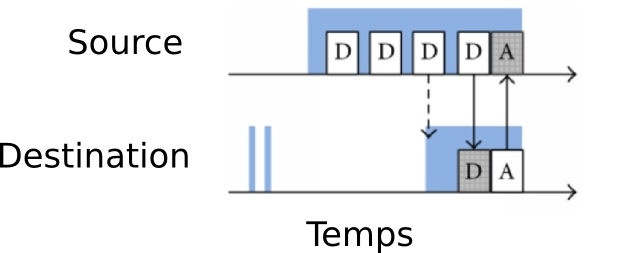
\includegraphics[width=.5\textwidth]{img/contikimac.png}
  \caption{Fonctionnement des réceptions avec ContikiMAC}
  \label{supervision:fig:contikimac}
\end{figure}

La Figure~\ref{supervision:fig:contikimac} illustre le fonctionnement de ContikiMAC.
Pour transmettre une trame de donnée (D), un émetteur l'envoie de manière répétée (``packet strobing'' en anglais) tant qu'une trame d'acquittement (A) n'est pas reçue de la part du récepteur.
Un récepteur va se réveiller périodiquement et faire une écoute du canal pour détecter la présence d'une trame (l'écoute du canal est représentée en bleu sur la figure).
Si aucune émission n'est détectée, le récepteur se rendort.
Quand une émission est détectée, le récepteur passe en réception pour recevoir la trame de donnée dans son intégralité puis, quand la trame de donnée est reçue, une trame d'acquittement est envoyée du récepteur vers l'expéditeur.

Dans le cas d'une trame destinée à tous les voisins (broadcast), elle est répétée sur toute la phase d'activité afin de s’assurer que tous les voisins l’ont reçue au moins une fois.
D'autre part, les voisins n'envoient pas un acquittement à la réception d'une trame envoyée en broadcast.

Si une trame est transmise sur le canal pendant la phase de réveil, le récepteur reste réveillé pour la recevoir sinon il se remet à l’état sommeil.
Lorsqu'un nœud reçoit une trame et qu'elle lui est effectivement destinée, il envoie un acquittement.

Pour optimiser sa transmission, le protocole ContikiMAC utilise une technique de verrouillage de phase.
Elle consiste à estimer la date de réveil du prochain saut pour une destination donnée à partir de la date de réception d’acquittement et de retarder le moment d’émission de paquets jusqu’à l’approche de cette date de réveil.
Cette technique peut économiser de l'énergie en réduisant la quantité de strobing nécessaire à l'envoi d'un paquet en ``synchronisant'' envois et phases de réveil.
Cependant, cette technique n'est pas parfaite, car les horloges internes des différents nœuds ne sont pas synchronisées et des décalages peuvent tout de même se produire~\cite{gonizzi2014rawmac}.

Toujours dans l’objectif d’augmenter la durée de la période de sommeil, le protocole ContikiMAC dispose d'un mécanisme de mise en sommeil rapide pouvant distinguer une transmission de paquet du bruit en comparant la période de l’activité à des longueurs types: (supérieure à la longueur maximale d’un paquet, etc.).
Si la période d'activité n'est pas due à une transmission, le nœud se rendort immédiatement.

Ainsi ContikiMAC permet d'économiser de l'énergie par de multiples techniques, mais cette économie se paye par l'envoi répété d'une trame.
Donc, il est nécessaire de comptabiliser ces retransmissions afin d'avoir une mesure implicite pertinente.

Soit $N_{\textrm{sender}}$ (respectivement $N_{\textrm{receiver}}$) le nombre de fois qu'une source (respectivement une destination) va transmettre (respectivement recevoir) un paquet avec ContikiMAC.

Puisque le destinataire se réveille en moyenne au milieu d'une transmission et attend le prochain essai d'envoi pour recevoir la trame complètement et envoyer son acquittement, le nombre de trames reçues par le destinataire peut être estimé à $N_{\textrm{receiver}} = 1.5$.

Estimer $N_{\textrm{sender}}$ est plus difficile, car cette grandeur dépend des conditions réseau (topologie, qualité du lien) et de la taille des trames.
Ainsi il est nécessaire d'avoir une estimation de ce paramètre afin de procéder à une estimation réaliste de l'utilisation de la radio.

L'expérience suivante est réalisée afin d'estimer le nombre moyen d'essais d'envoi d'une trame de donnée qu'un expéditeur va faire avant de recevoir une trame de confirmation.
Deux nœuds utilisant ContikiMAC sont mis à portée de transmission dans un environnement non bruité.
La source envoie en boucle un paquet de taille fixe qui induit de multiples retransmissions, puis elle attend l'acquittement du paquet et comptabilise le nombre d'essais réalisés avant de recevoir un acquittement et cela pour différentes tailles de paquets.
\ieee{} est utilisé comme simple couche liaison avec un entête pour les trames de données aussi réduit que possible (6 octets) les différentes tailles de trames sont obtenues en faisant varier la taille du message applicatif.
Une simulation simule le comportement de ce système pendant 10000 secondes et pour chaque taille de paquet, l'expérience est exécutée 10 fois avec une graine de générateur de nombre aléatoire différente à chaque fois.

\begin{figure}[h]
  \centering
  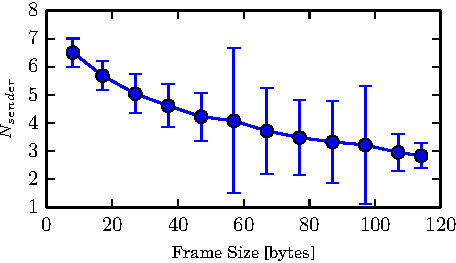
\includegraphics[width=.5\textwidth]{img/average_strobbing-crop.pdf}
  \caption{Nombre moyen de tentatives d'envois en fonction de la taille de la trame avec ContikiMAC.}
  \label{supervision:fig:average_strobing}
\end{figure}

La Figure~\ref{supervision:fig:average_strobing} représente la moyenne du nombre de transmissions $N_{\textrm{sender}}(f)$ nécessaires à l'envoi d'une trame $f$ ayant une taille de $\mathcal{L}(f)$ octets entre deux nœuds fonctionnant avec ContikiMAC.
Le nombre d'envois moyens nécessaires pour envoyer un long paquet est plus faible que pour en envoyer un court, car les trames longues mettent plus de temps pour être transmises et ont donc plus de chance d'être écoutées pendant un réveil du destinataire.
% En outre, comme les paquets \ac{ACK} ont une taille constante, le coût de réception pour la source est constant.
% Cette valeur est inférieure à celle de $N_{\textrm{receiver}}$ ainsi c'est donc l'expéditeur qui va dépenser le plus d'énergie quand ContikiMAC est employé.

On peut remarquer que la variance est également faible pour des trames de grande taille ce qui est également cohérent, car le nombre d'envois qu'il est possible de faire pour une trame de cette taille au cours d'un cycle complet est limité ainsi la variance est réduite. 

\section{Validation expérimentale}
\label{supervision:validation}

\subsection{Supervision passive}
\label{supervision:chain_results}

\begin{figure}[ht]
  \centering
  \begin{tikzpicture}

  % définition des styles
  \tikzstyle{child}=[circle, draw, fill=yellow!50,text=black]
  \tikzstyle{router}=[circle, draw, fill=orange!50,text=black]
  \tikzstyle{root}=[circle, draw, fill=red!50,text=black]

  % Réseau contraint
  \node[root] (root) {G};
  \node[router, left=of root] (1) {1};
  \node[router, left=of 1] (2) {2};
  \node[router, left=of 2] (3)  {3};
  \node[router, left=of 3] (4) {4};
  \node[router, left=of 4] (5) {5};
  \node[child, left=of 5] (6) {6};

\path

  (6.east) edge[->, thin] (5.west)
  (5.east) edge[->, thin] (4.west)
  (4.east) edge[->, semithick] (3.west)
  (3.east) edge[->, thick] (2.west)
  (2.east) edge[->, very thick] (1.west)
  (1.east) edge[->, ultra thick] (root.west)
  ;

  \end{tikzpicture}

  \caption{Topologie réseau utilisée pour mesurer la précision de la mesure implicite et passive}

  \label{supervision:fig:topology_chain}
\end{figure}

Une topologie chaînée à 7 nœuds comme représentée sur la Figure~\ref{supervision:fig:topology_chain} est utilisée pour tester le mécanisme décrit ci-dessus.
Dans cette configuration, les nœuds ne peuvent envoyer et recevoir de  paquets que de la part de leurs voisins adjacents.
Tous les paquets remontent vers la passerelle représentée par un G sur la figure.

Les nœuds utilisent le système Contiki~\cite{dunkels2004contiki}, \ieee{} pour communiquer et ContikiMAC comme mécanisme de cycle de veille.
\ac{RPL}~\cite{rfc6550} est le protocole de routage utilisé et il est configuré en non-storing mode, c'est-à-dire qu'il a accès à toute la topologie réseau et en particulier aux routes descendantes.

Durant 200 secondes, chaque nœud envoie au \ac{LBR} un paquet \ac{UDP} à chaque seconde avec une charge utile de 10 octets ce qui induit une trame de 69 octets chaque seconde.
Le trafic applicatif d'un nœud démarre lorsqu'il joint la topologie réseau, il a alors un parent qui est son voisin adjacent.

D'après les résultats expérimentaux (Figure. \ref{supervision:fig:average_strobing}), l'utilisation de ContikiMAC induit qu'une trame de 69 octets est émise en moyenne 3,76 fois avant d'être reçue.
Le mécanisme de mesure implicite tient compte de ce phénomène et l'applique à chaque routeur intermédiaire afin que l'utilisation de la radio soit en accord avec ce résultat.

Les temps de transmission et de réception des nœuds sont obtenus par l'utilisation du simulateur et de Powertracker~\cite{dunkels2011powertrace} qui permet d'obtenir le temps passé dans chaque état de transmission radio pour chaque nœud avec une résolution de $1 \mu s$.
Puisque la passerelle est toujours éveillée, elle reçoit donc du premier coup toutes les trames: $N_{\textrm{receiver}} = 1$.

\subsubsection{Analyse de l'impact de la profondeur}
\label{supervision:depth_analysis}

\begin{figure}[ht]
  \begin{subfigure}{0.5\textwidth}
    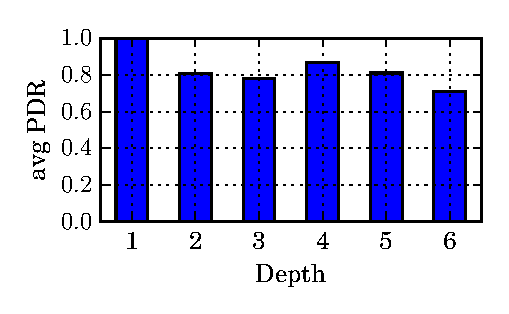
\includegraphics[width=\textwidth]{img/pdr_depth.pdf}
    \caption{Packet Delivery Ratio (PDR).}
    \label{supervision:fig:pdr_depth}
  \end{subfigure}
  \begin{subfigure}{0.5\textwidth}
    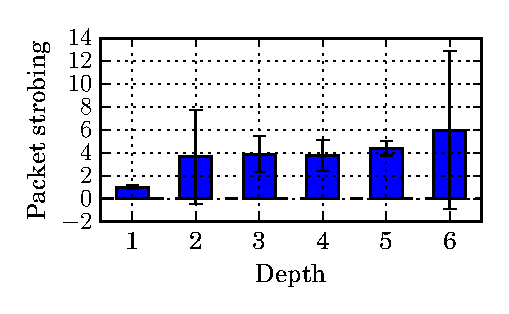
\includegraphics[width=\textwidth]{img/strobes_depth.pdf}
    \caption{Tentatives d'envois de paquets par profondeur.}
    \label{supervision:fig:strobes_depth}
  \end{subfigure}
  \caption{Impact de la profondeur}
\end{figure}

\paragraph{\ac{PDR}}

La figure Fig.~\ref{supervision:fig:pdr_depth} représente le ratio de succès de transmission de paquets applicatifs pour chaque nœud en fonction de la distance à la racine en nombre de sauts.
Cette figure montre la proportion du trafic applicatif que la passerelle peut effectivement voir.
Le ratio de paquets acheminés n'est pas uniforme sur tout le \ac{LLN} et les nœuds qui ne sont pas connectés directement à une racine souffrent de pertes de paquets non négligeables malgré un trafic faible en raison d'un grand nombre de retransmissions de paquets.

Le routeur de bordure n'utilise pas ContikiMAC car dans les hypothèses de l'expérience, il n'est pas contraint en énergie et peut donc rester éveillé en permanence.
Ainsi, tous les paquets issus du nœud 1 sont reçus prouvant que ContikiMAC induit des pertes et nuit à la fiabilité des transmissions pour les nœuds plus éloignés.

Puisqu'un paquet peut être perdu à chaque fois qu'il traverse un routeur fonctionnant avec ContikiMAC, traverser de nombreux routeurs augmente la probabilité que les paquets soient perdus, car \ac{UDP} ne fournit aucun mécanisme de fiabilité.
Ce phénomène est confirmé par la Figure~\ref{supervision:fig:pdr_depth} où la quantité de paquets arrivant à la racine semble décroître globalement à mesure qu'on s'en éloigne.

\paragraph{Retransmissions de paquets (``Packet strobing'')}

La Figure~\ref{supervision:fig:strobes_depth} représente le nombre moyen d'envois de paquets i.e. le nombre de tentatives que va faire chaque nœud pour envoyer une trame à son parent.

Les valeurs obtenues précédemment restent expérimentalement proches de la valeur de 3,76 obtenue expérimentalement (Figure \ref{supervision:fig:average_strobing}).
Cependant, la variance est forte et le nombre de tentatives tend à augmenter à mesure que l'on s'éloigne de la racine.
Cette variance peut être expliquée par la variance obtenue pour des trames de 69 octets sur l'expérience de calcul des $N_{sender}$.

La convergence vers la valeur normale de 3,76 pour les nœuds proches de la racine s'explique par l'augmentation du trafic réseau sur ces nœuds: ils doivent relayer les paquets provenant de tous les autres nœuds.
Ainsi, leur rythme d'envoi se rapproche de celui de l'expérience de strobing où la source envoyait autant de paquets que possible vers un destinataire en s'assurant de son acquittement.
Pour un nœud situé en bout de chaîne et n'ayant donc aucune charge de routage, un plus grand décalage entre les cycles d'éveils est présent et explique ainsi les retransmissions supplémentaires.

Enfin, au sujet du nœud qui est connecté à la passerelle directement, la quantité moyenne d'envois est très proche de 1 avec une variance faible, ce qui est logique puisque par hypothèse la racine est toujours éveillée et peut donc recevoir immédiatement les transmissions qui en viennent.
Cependant, ce n'est pas le cas des nœuds se situant juste avant le nœud 1, qui reçoivent une quantité importante de trafic, mais qui ne peuvent pas la router avec la même efficacité (temporisation, ``buffering'', etc.).

\subsubsection{Analyse de l'impact des protocoles}
\label{supervision:protocols_analysis}

Connaître la répartition des protocoles au cours du temps permet de savoir la proportion de ressources investies dans le maintien du réseau et celle investie dans un but applicatif à valeur ajoutée.

\begin{figure}[ht]
  \begin{subfigure}{0.5\textwidth}
    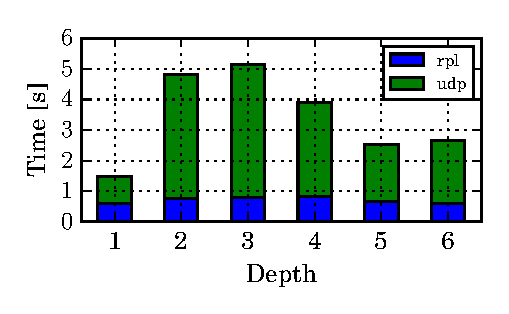
\includegraphics[width=\textwidth]{img/protocol_repartition_depth.pdf}
    \caption{Répartition des protocoles par profondeur.}
    \label{supervision:fig:protocol_repartition}
  \end{subfigure}
  \begin{subfigure}{0.5\textwidth}
    \centering
    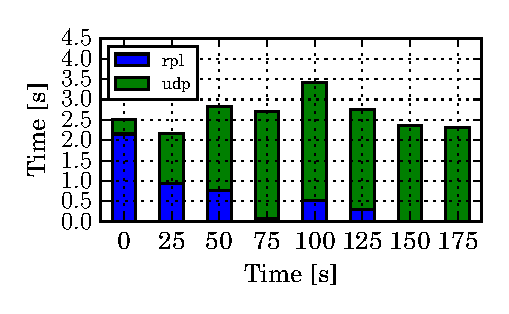
\includegraphics[width=\textwidth]{img/repartition_protocol.pdf}
    \caption{Évolution de la répartition des protocoles (statistiques par fenêtres de 25 secondes.}
    \label{supervision:fig:protocol_repartition_time}
  \end{subfigure}%
  \caption{Impact des protocoles}
\end{figure}

\paragraph{Répartition des protocoles}

La Figure~\ref{supervision:fig:protocol_repartition} met en évidence que la quantité de trafic lié au protocole de routage est relativement homogène pour tous les nœuds.
Ce phénomène est lié à la topologie et au fonctionnement de \ac{RPL}: les nœuds n'envoient de paquets de routage qu'à un seul parent à la fois ainsi le trafic de routage est le même pour tous les nœuds du réseau.

\paragraph{Évolution au cours du temps}

La Figure~\ref{supervision:fig:protocol_repartition_time} met en évidence l'évolution typique de la répartition des protocoles au cours du temps.
La charge liée au protocole de routage est très importante lors du démarrage du réseau, car aucune route n'est alors disponible.
Ainsi l'essentiel du trafic observé correspond à des paquets \ac{RPL} qui sont utilisés pour mettre à jour les routes sur chaque nœud.

\ac{RPL} étant proactif, les routes sont construites et entretenues en permanence, ainsi même après la construction de la topologie, du trafic \ac{RPL} est toujours émis.
Cependant, le mécanisme de ``Trickle'' réduit la quantité de paquets émis pour maintenir la topologie qui est observée.

Cette évolution du trafic permet de déduire qu'un mécanisme n'ayant pas la connaissance des routes manquerait non seulement l'impact du relayage sur les routeurs dans la topologie, mais aussi la charge impliquée par la construction des routes qui est non négligeable même dans le cas d'une topologie simple comme celle d'une chaîne.

Cependant, le trafic applicatif est majoritaire lorsque le réseau est stable, ainsi l'approche par supervision passive peut être explorée, car l'essentiel du trafic a vocation à passer par le routeur de bordure.

\subsection{Précision de la mesure passive de l'utilisation de la radio}

Le mécanisme d'estimation se déclenche quand toutes les routes sont établies et qu'un trafic réseau est observé à la passerelle.
L'estimation du temps radio va alors fournir une estimation pour le temps passé en transmission et en réception pour chaque nœud.

On appelle \emph{précision} $\delta = \frac{\widehat{X}}{X}$ le rapport entre l'estimation d'une grandeur $\widehat{X}$ et sa valeur réelle $X$ qui est mesurée dans le simulateur.
Cette métrique permet d'interpréter facilement les grandeurs trouvées: $\delta \leq 1$ (respectivement $\delta \geq 1$) signifie que l'estimation sous-estime (respectivement surestime) la grandeur.
Cette section mesure la précision des estimations passives pour les cas d'estimation ``étoilée'' (où la topologie de routage est inconnue) et ``maillée'' (où la topologie de routage est connue).

\subsubsection{Précision en fonction de la topologie}

\begin{figure}[ht]
  \begin{subfigure}{0.5\textwidth}
    \centering
    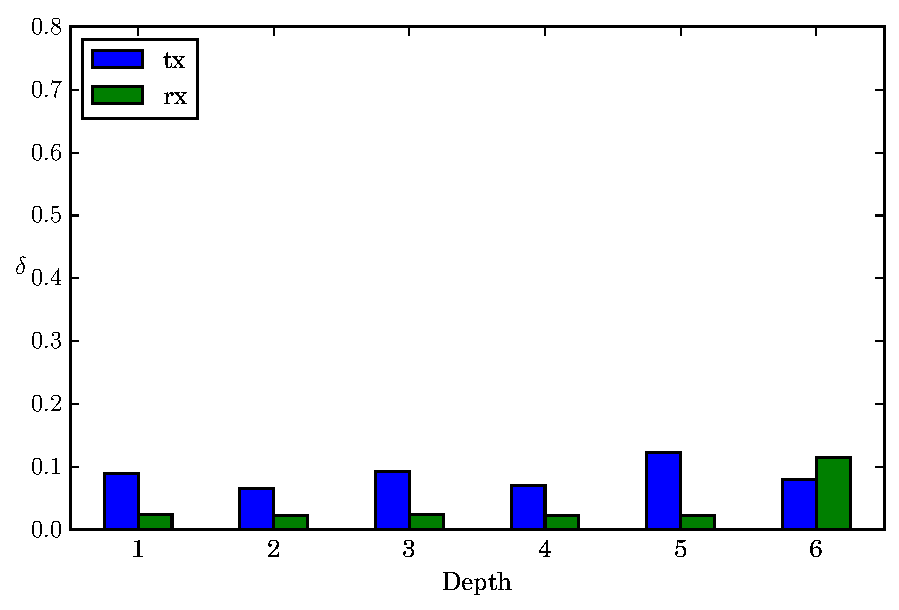
\includegraphics[width=\textwidth]{img/global_noinfo.pdf}
    \caption{$\delta$ total global pour l'estimation ``étoilée''}
    \label{supervision:fig:global_noinfo}
  \end{subfigure}
  \begin{subfigure}{0.5\textwidth}
    \centering
    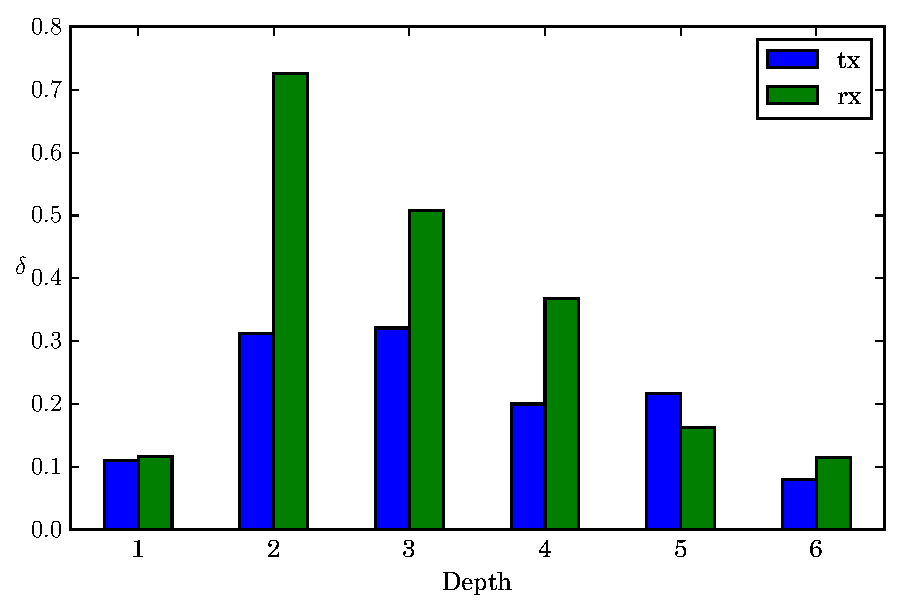
\includegraphics[width=\textwidth]{img/global_route.pdf}
    \caption{$\delta$ total global pour l'estimation ``maillée''}
    \label{supervision:fig:global_route}
  \end{subfigure}
  \caption{$\delta$ total et global par profondeur}
  \label{supervision:fig:global}
\end{figure}

La Figure~\ref{supervision:fig:global} montre que la précision obtenue à la fin de la simulation pour chaque nœud est sous-estimée.
Ce phénomène est attendu, car la mesure implicite ne peut inférer tous les phénomènes, de plus l'approche proposée n'introduit pas de mécanismes ad hoc pour augmenter les estimations.

Dans le cas de l'estimation ``étoilée'', $\delta$ est homogène pour l'ensemble des nœuds qui ont pour charge de router des paquets qui ne leur sont pas destinés comme le montre la Figure~\ref{supervision:fig:global_noinfo}.
C'est cohérent avec la nature de l'estimation ``étoilée'' qui ne prend pas en compte toute la charge liée au routage.
De plus, la réception est plus sous-évaluée que la transmission, car elle ne prend en compte que la réception des trames d'acquittement qui représentent un volume très restreint sauf pour le nœud 6 qui n'a pas d'autre charge de réception.

Dans le cas de l'estimation ``maillée'', $\delta$ est plus élevé, car l'utilisation de la radio liée aux retransmissions est prise en charge ainsi une plus grande part du trafic est déduite des observations passives.
On remarque un net progrès pour la réception qui d'une part est régulière à prévoir avec ContikiMAC ($N_{receiver} = 1.5$) et d'autre part parce que le volume de routage est plus important.

Les erreurs d'estimations restent cependant importantes, car dans les deux cas, une part importante du trafic n'est pas inféré (pertes de paquets, variance du strobbing, trafic de routage local non transmis à la passerelle, etc.).

En outre, la mesure implicite ``étoilée'' ou ``maillée'' est identique pour le nœud feuille par construction, car aucune charge de routage ne lui est appliqué dans les deux cas.

\subsubsection{Évolution de $\delta$ au cours du temps}

Cette section étudie l'évolution de $\delta$ au cours du temps afin d'affiner la compréhension des facteurs pouvant expliquer la sous-estimation obtenue dans la section précédente.
Les résultats suivants sont obtenus en découpant l'expérience sur des intervalles de 20 secondes.
$\delta$ est alors le temps de radio estimé sur le temps réel dans cet intervalle uniquement.

\paragraph{Estimation ``étoilée''}

\begin{figure}[h]
  \centering
  \begin{subfigure}{0.3\textwidth}
    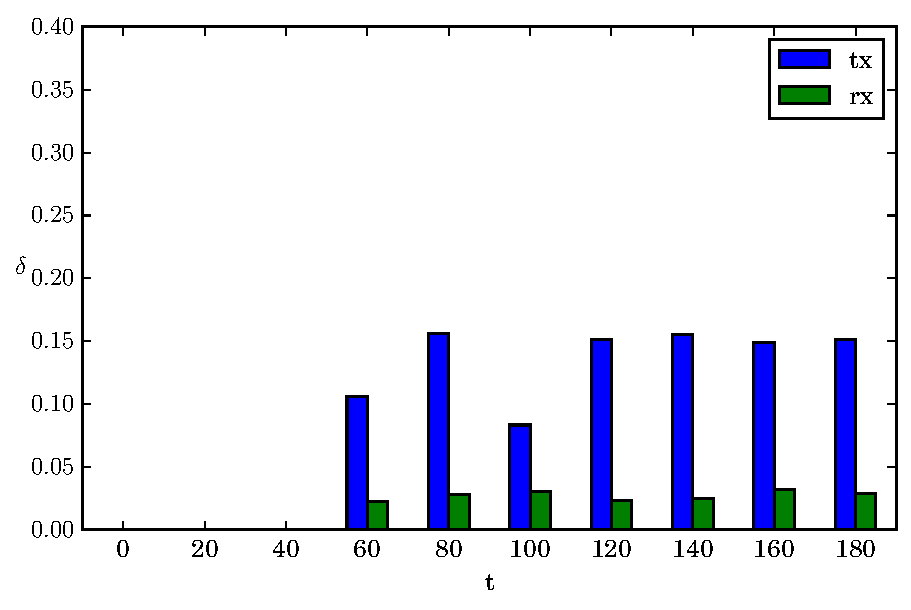
\includegraphics[width=\textwidth]{img/evolution_noinfo_1.pdf}
    \caption{Profondeur: 1}
    \label{supervision:fig:noinfo_1}
  \end{subfigure}
  \begin{subfigure}{0.3\textwidth}
    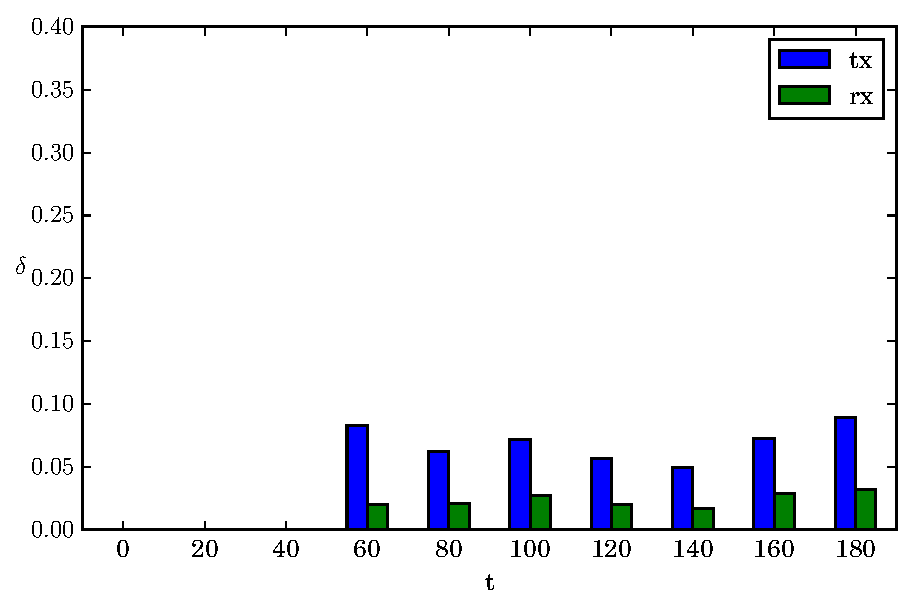
\includegraphics[width=\textwidth]{img/evolution_noinfo_2.pdf}
    \caption{Profondeur: 2}
    \label{supervision:fig:noinfo_2}
  \end{subfigure}
  \begin{subfigure}{0.3\textwidth}
    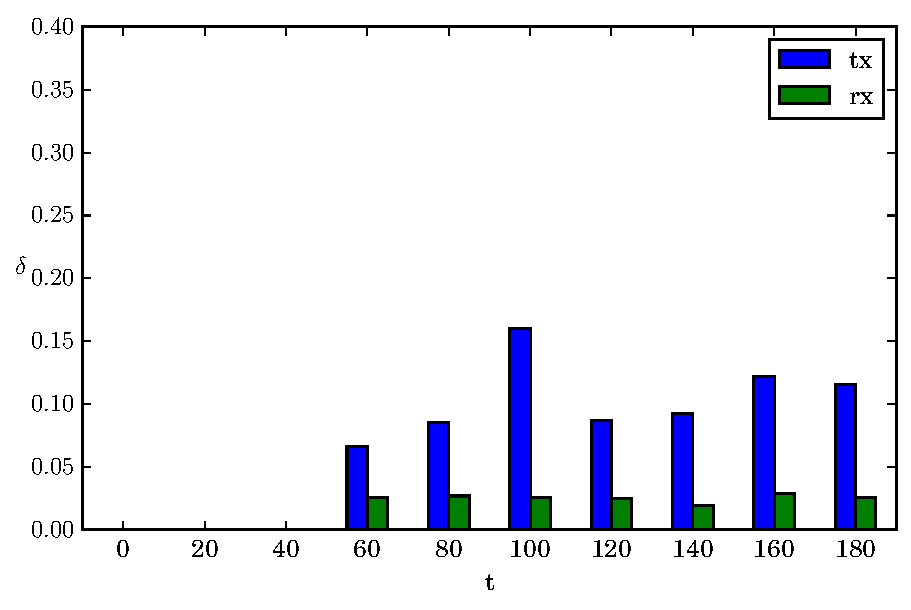
\includegraphics[width=\textwidth]{img/evolution_noinfo_3.pdf}
    \caption{Profondeur: 3}
    \label{supervision:fig:noinfo_3}
  \end{subfigure}

  \begin{subfigure}{0.3\textwidth}
    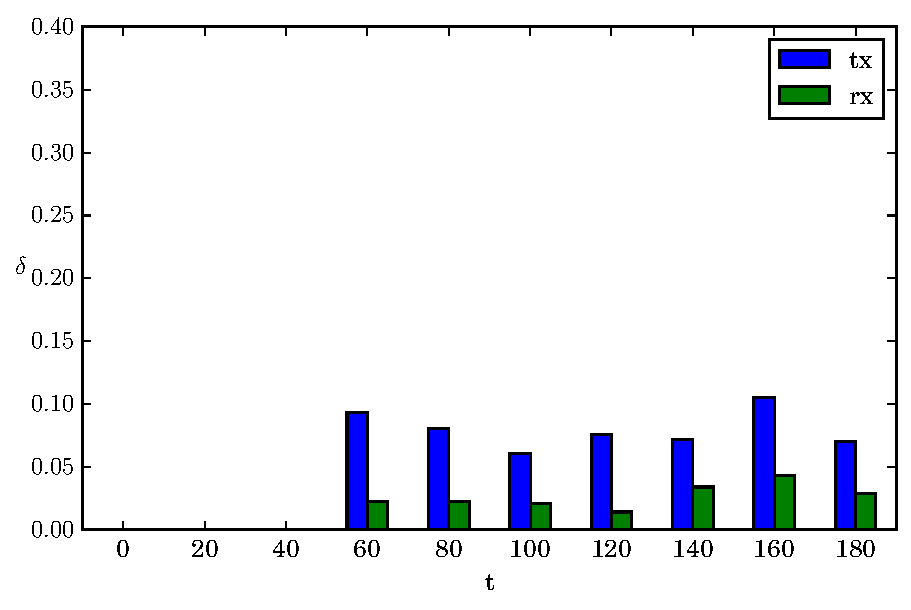
\includegraphics[width=\textwidth]{img/evolution_noinfo_4.pdf}
    \caption{Profondeur: 4}
    \label{supervision:fig:noinfo_4}
  \end{subfigure}
  \begin{subfigure}{0.3\textwidth}
    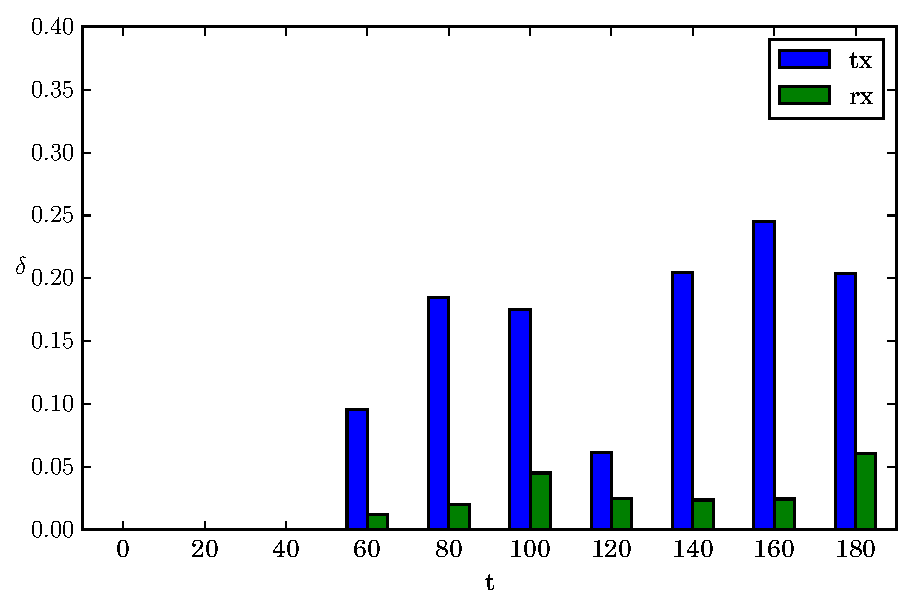
\includegraphics[width=\textwidth]{img/evolution_noinfo_5.pdf}
    \caption{Profondeur: 5}
    \label{supervision:fig:noinfo_5}
  \end{subfigure}
  \begin{subfigure}{0.3\textwidth}
    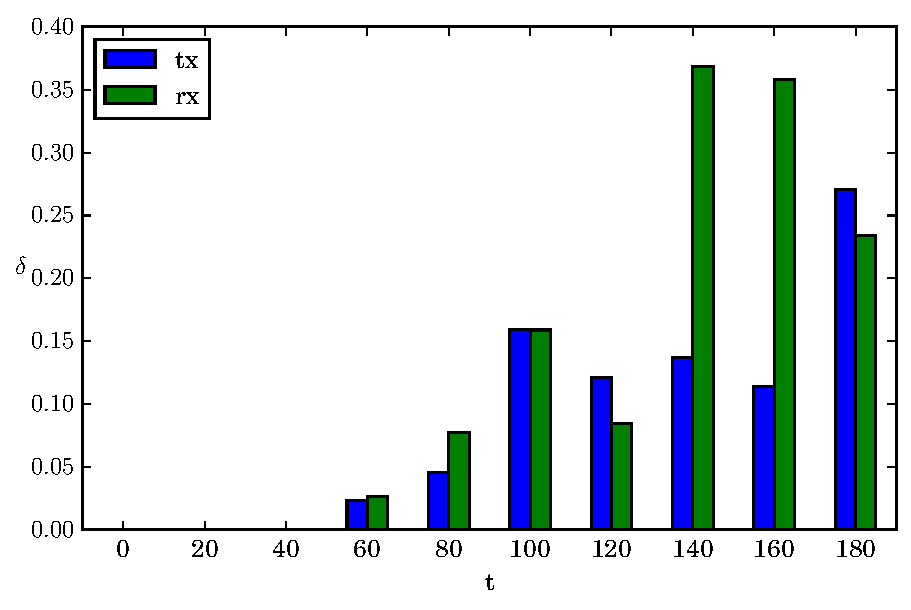
\includegraphics[width=\textwidth]{img/evolution_noinfo_6.pdf}
    \caption{Profondeur: 6}
    \label{supervision:fig:noinfo_6}
  \end{subfigure}
  \caption{Évolution de $\delta$ pour une estimation ``étoilée''}
  \label{supervision:fig:noinfo}
\end{figure}

La Figure~\ref{supervision:fig:noinfo} détaille pour chaque nœud l'évolution de $\delta$ pour une estimation ``étoilée''.
La sous-estimation continue, car les processus non visible depuis la passerelle (routage des paquets, pertes de paquets, etc.) continuent au cours de l'expérience.

Les nœuds situés à une plus grande profondeur relaient moins de paquets ainsi leur $\delta$ augmente, car une plus grande proportion de leur trafic applicatif est connue par le routeur de bordure au fur et à mesure de l'expérience.
D'autre part, $\delta$ augmente au cours du temps, car le trafic applicatif qui est celui inféré par la mesure passive prend une part plus importante au cours du temps (\ref{supervision:fig:protocol_repartition_time}).

\paragraph{Estimation ``maillée''}

\begin{figure}[h]
  \centering
  \begin{subfigure}{0.3\textwidth}
    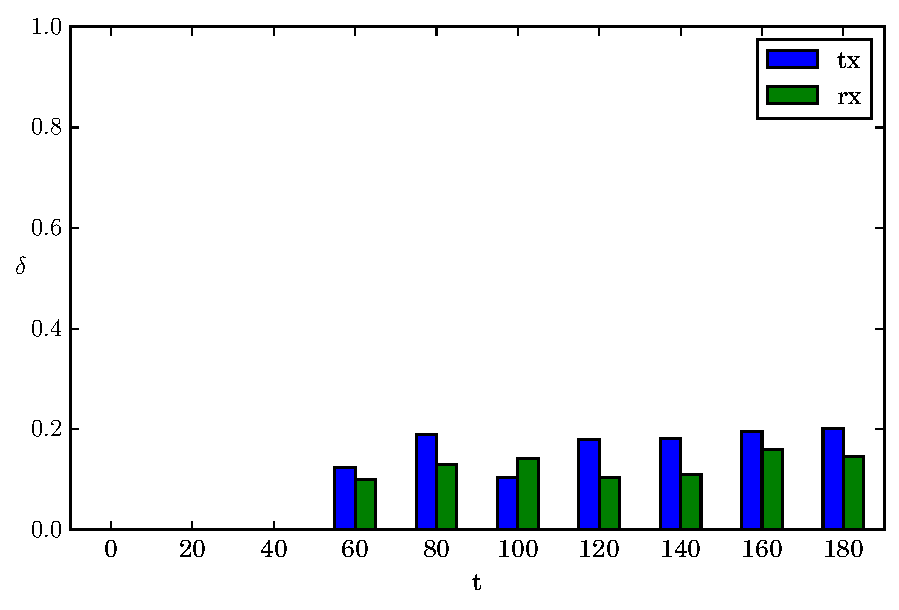
\includegraphics[width=\textwidth]{img/evolution_route_1.pdf}
    \caption{Profondeur: 1}
    \label{supervision:fig:route_1}
  \end{subfigure}
  \begin{subfigure}{0.3\textwidth}
    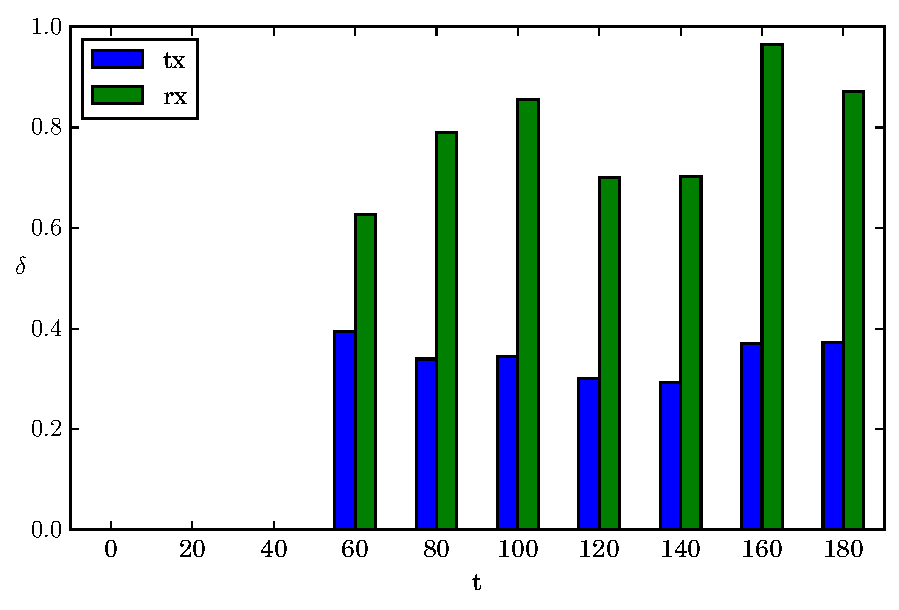
\includegraphics[width=\textwidth]{img/evolution_route_2.pdf}
    \caption{Profondeur: 2}
    \label{supervision:fig:route_2}
  \end{subfigure}
  \begin{subfigure}{0.3\textwidth}
    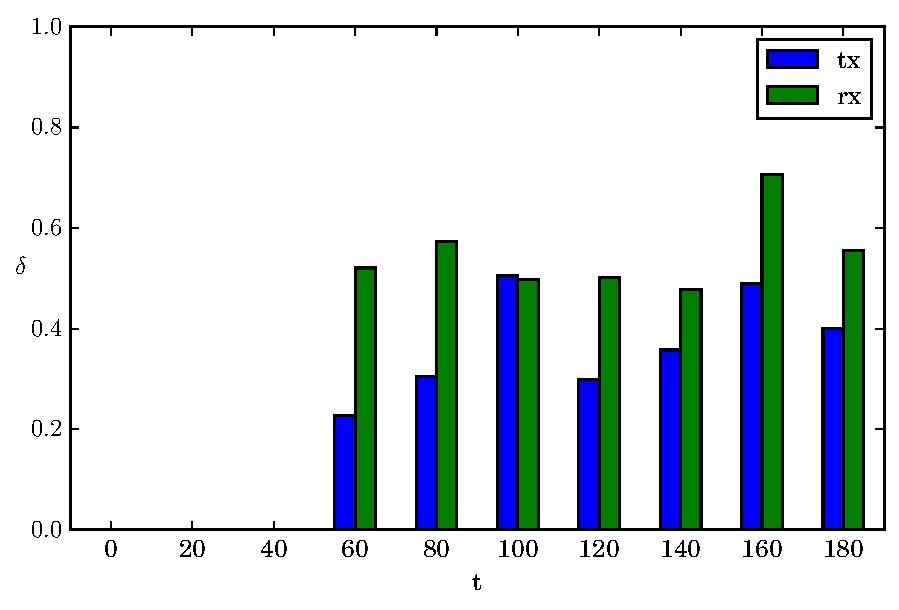
\includegraphics[width=\textwidth]{img/evolution_route_3.pdf}
    \caption{Profondeur: 3}
    \label{supervision:fig:route_3}
  \end{subfigure}

  \begin{subfigure}{0.3\textwidth}
    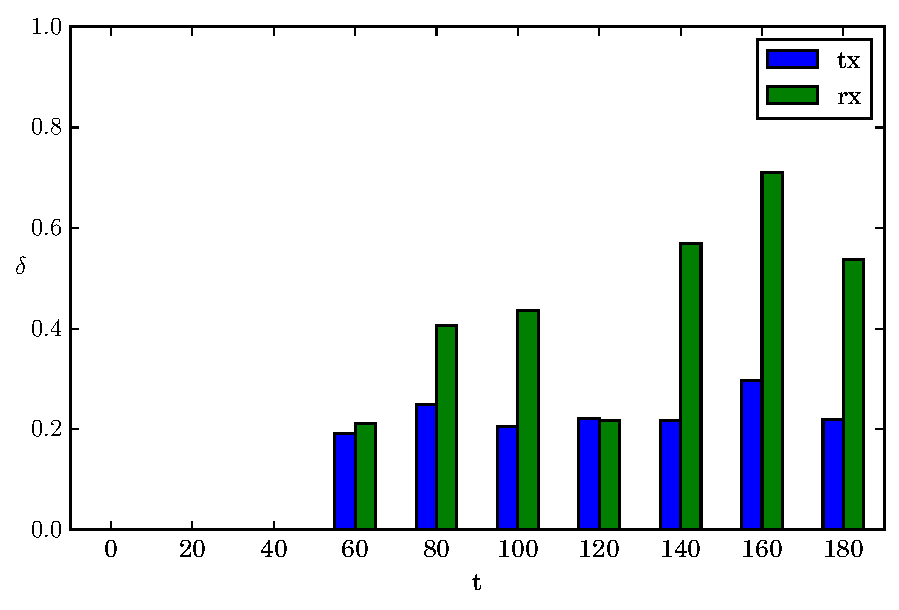
\includegraphics[width=\textwidth]{img/evolution_route_4.pdf}
    \caption{Profondeur: 4}
    \label{supervision:fig:route_4}
  \end{subfigure}
  \begin{subfigure}{0.3\textwidth}
    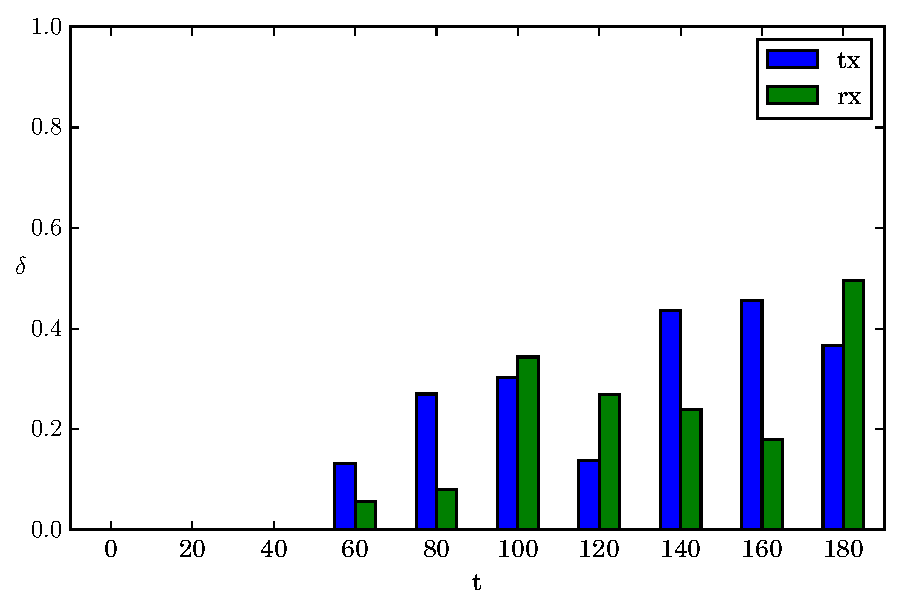
\includegraphics[width=\textwidth]{img/evolution_route_5.pdf}
    \caption{Profondeur: 5}
    \label{supervision:fig:route_5}
  \end{subfigure}
  \begin{subfigure}{0.3\textwidth}
    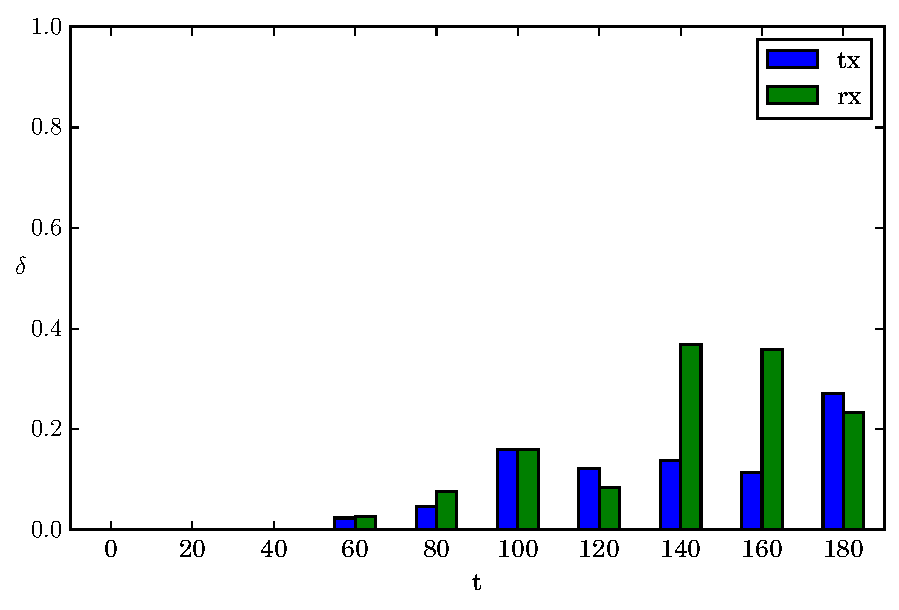
\includegraphics[width=\textwidth]{img/evolution_route_6.pdf}
    \caption{Profondeur: 6}
    \label{supervision:fig:route_6}
  \end{subfigure}
  \caption{Évolution de l'$\delta$ pour une estimation ``maillée''}
  \label{supervision:fig:route}
\end{figure}

L'estimation maillée est meilleure sur tous les intervalles de temps, ce qui est attendu, car elle comptabilise la charge de routage sur chacun de ces intervalles en plus de l'estimation étoilée.

D'autre part, l'estimation s'améliore au cours du temps, car non seulement le trafic applicatif devient majoritaire au cours du temps comme montré sur la Figure~\ref{supervision:fig:protocol_repartition_time} mais en plus la charge de routage intermédiaire qu'il induit est également comptabilisée.

% Discussion

Cependant, l'erreur d'estimation est encore forte en raison des pertes de paquets et des variations de la quantité de ``strobbing'' nécessaire pour transmettre un paquet à chaque saut.
Ainsi si la quantité de strobbing est sous-estimée, sur chaque saut l'impact de chaque paquet sur l'estimation de la radio est grandement perturbé.

Afin de limiter le strobbing, une solution serait d'avoir des trames aussi remplies que possible (par exemple avec des informations au sujet des nœuds.).
Ainsi, la quantité de strobbing nécessaire serait beaucoup plus faible, car les trames seraient détectées au bout d'un faible nombre de tentatives.

Une autre solution possible consiste à envoyer à intervalles réguliers des informations de ``recalibrations'' afin de recaler les estimations pour fournir des valeurs correctes.

\section{Mesures explicites}
\label{supervision:explicite}

La passerelle peut effectuer une mesure passive du temps passé par les nœuds du \ac{LLN} en transmission et en réception.
Cependant, les paquets perdus, retransmis ou non routés vers la passerelle ne sont pas comptabilisés avec cette méthode qui induit donc un biais.

Ainsi des mécanismes de mesure active semblent inévitables pour obtenir une information fiable.
Ces messages peuvent être envoyés à la passerelle par ``piggybacking'' ou être mis dans les paquets du protocole de routage utilisé.

Cependant, le rythme de ces mesures doit être modéré afin de limiter la consommation de ressources qu'il induit.
Ainsi si les temps entre deux envois de mesures explicites sont longs, la mesure implicite de la radio précédemment introduite peut fournir une approximation entre ces deux envois.

Quand la passerelle reçoit une mesure explicite au temps $t$ elle recalcule son estimation pour la grandeur $\widehat{X}$ de la manière suivante:

\begin{align}
  \widehat{X}(t) &= X(t_r) + \epsilon(t_r)\frac{t - t_r}{T}\\
  \epsilon(t_r) &= \alpha (X(t_r) - \widehat{X}(t_r)) + (1 - \alpha)\epsilon(t_{r-1})
  \label{supervision:eqn:bias}
\end{align}

où $t_r$ et $t_{r-1}$ sont les deux dernières dates de réception de mesure active.
$T$ désigne le temps entre chaque mesure explicite reçue.
$X(t_r)$ désigne la valeur obtenue par mesure explicite à l'instant $t_r$.
$\epsilon(t_r)$ est l’estimation de l'erreur apprise des précédents messages de mesure active~\footnote{Par convention: $\epsilon(0) = 0$}.
Cette erreur est calculée par une \ac{EWMA} de paramètre $\alpha$~\cite{mckinney2012python}.
Le coefficient $\alpha$ compris entre 0 et 1 représente le degré de décroissance des erreurs des valeurs passées.
Une valeur de $\alpha$ importante réduira plus rapidement l'importance des observations passées.
A un instant $t$, l'erreur est prise proportionnellement au temps depuis la dernière mesure explicite reçue.


% $\frac{X(t_r) - X(t_{r-1})}{t_r - t_{r-1}}$ représente la tendance de la grandeur $X$. 
% Le paramètre $\alpha$ désigne la proportion de l'estimation 

\subsection{Validation expérimentale}

\begin{figure}[ht]
  \centering
  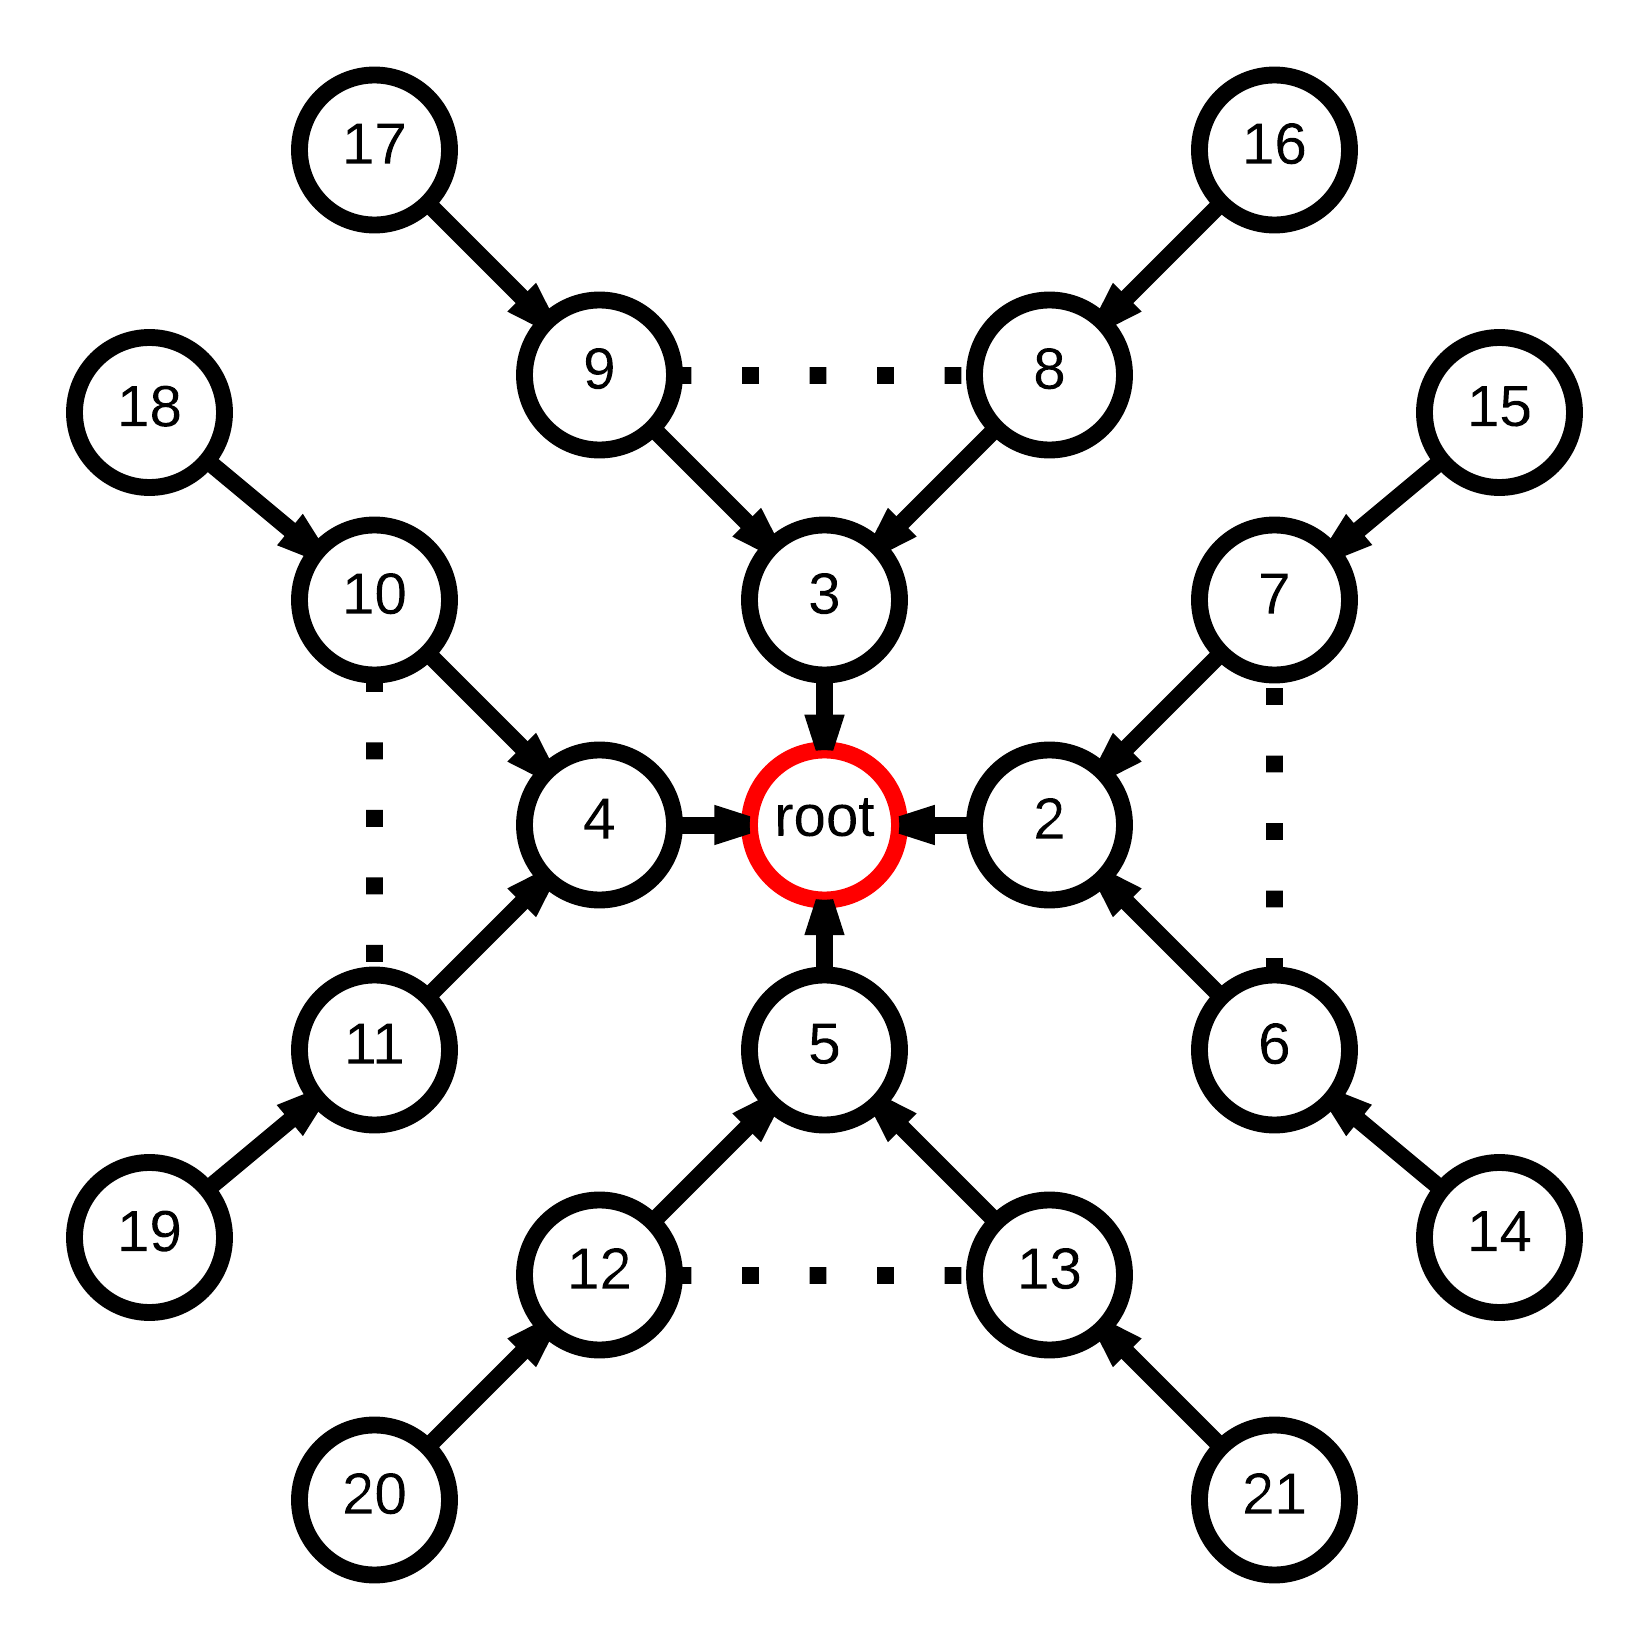
\includegraphics[width=0.5\textwidth]{img/topology_tree.png}
  \caption{Topologie réseau et radio.}
  \label{supervision:fig:topology_tree}
\end{figure}

Cette méthode de recalibration des mesures passives est évaluée en utilisant une topologie représentée sur la Figure~\ref{supervision:fig:topology_tree} composée de 21 nœuds envoyant des paquets applicatifs à la racine chaque seconde pendant 200 secondes.
Les messages contenant des mesures exactes des temps mesurés par le nœud passé dans chaque état de transmission sont envoyés par les nœuds par un mécanisme de publish-subscribe pour économiser le coût d'une requête.
La fréquence de ces envois de recalibrations est réglée par l'administrateur.

Comme vu dans les validations précédentes, le réseau est peu régulier et les phénomènes de strobing ont une grande variance.
Ainsi, afin de ne pas réagir trop brutalement aux changements d'une mesure et de privilégier les tendances de fond, le paramètre de décroissance de l'\ac{EWMA} est mis à $\alpha = 0.25$.

\paragraph{Erreur relative globale}

\begin{figure}[ht]
  \centering
  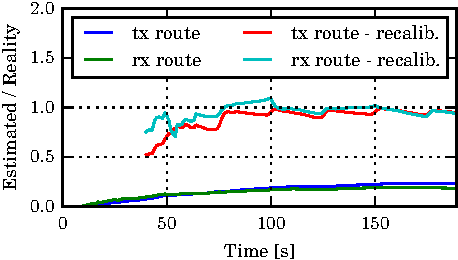
\includegraphics{img/ratio_recalibration_global-crop.pdf}
  \caption{Erreur d'estimation globale pour une topologie en arbre avec et sans recalibration dynamique (toutes les 25 secondes).}
  \label{supervision:fig:tree_calibration}
\end{figure}

La Figure~\ref{supervision:fig:tree_calibration} montre le rapport entre la valeur estimée et la valeur réelle moyenne quand des messages de supervisions périodiques sont envoyés par les nœuds toutes les 25 secondes.
A chaque mesure explicite, l'estimateur intègre l'erreur moyenne des précédentes mesures et converge ainsi vers une estimation correcte.
On observe également que les pentes des estimations après chaque recalibrations sont moins grandes, car l'estimateur apprend son biais qui est supposé constant pendant l'expérience.
Ainsi on obtient une estimation qui a tout temps est capable de produire une estimation du temps passé en transmission et en réception.

\paragraph{Fréquence de recalibrage}

\begin{figure}[ht]
  \centering
  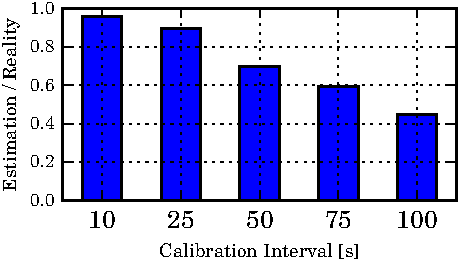
\includegraphics{img/ratio_recalibration-crop.pdf}
  \caption{Erreur relative pour différents intervalles de supervision active.}
  \label{supervision:fig:frequencies_error}
\end{figure}

La Figure~\ref{supervision:fig:frequencies_error} montre l'erreur moyenne globale obtenue par le mécanisme avec une estimation étoilée en fonction des périodes entre chaque message de supervision active.
Sur une expérience durant 200 secondes, n'avoir qu'une seule recalibration à mi-parcours (100 secondes) n'est pas suffisant pour avoir une bonne précision.
Ce phénomène est attendu, car même si la mesure active permet de connaître l'état exact d'un nœud, n'avoir cette information qu'une fois au cours de l'expérience n'est pas suffisant.
Lorsque les recalibrations sont plus fréquentes, la précision est meilleure, mais au prix d'un plus grand nombre de paquets émis.

\subsection{Travaux en cours}
\label{supervision:ingoing}

De nouveaux travaux~\footnote{Entrepris lors d'un séjour au \ac{SICS} entre août et septembre 2015 en collaboration avec Simon Duquennoy.} étendent les recherches de ce chapitre.
Leur objectif est de trouver des schémas de supervision explicites plus économes en énergie que les méthodes systématiques et cycliques présentes dans l'état de l'art.
Partant du constat que la supervision active est toujours nécessaire et ne peut pas être facilement substituée, l'objectif consiste à trouver une méthode optimale de supervision permettant de réduire son coût autant que possible.

\subsubsection{Mesure systématique}

Une supervision cyclique impose à chaque nœud d'envoyer des rapports sur son état à intervalles réguliers.
Le problème de cette approche est que son coût augmente linéairement avec le nombre de nœuds présents dans le \ac{LLN} et peut être coûteux en ressources si la fréquence d'envoi est trop importante.

Une première piste de recherche en cours d'investigation consiste à diminuer le nombre d'informations envoyées à mesure que le comportement d'un nœud est stable.
Cette méthode s'inspire de la méthode utilisée par Trickle~\cite{rfc6206} dans le protocole \ac{RPL} qui diminue le nombre de messages de routage à mesure que le routage devient stable.
L'évaluation de cette méthode notamment dans le cas de réseau instable et la comparaison avec des méthodes cycliques est l'un des premiers objectifs de ces nouveaux travaux.

\subsubsection{Mesure ciblée dynamique}

Une seconde approche consiste à choisir dynamiquement quel nœud interroger afin d'améliorer le modèle que la passerelle a d'un \ac{LLN}.
Cependant, la passerelle ne peut savoir si l'état d'un nœud diverge de son modèle avant de le lui demander.
Ainsi la passerelle a le choix entre conserver un modèle incertain et ne pas solliciter un nœud donné afin d'économiser des ressources ou bien payer le coût d'une mesure active quitte à ce qu'elle ne soit pas pertinente.
Cette problématique d'exploration contre exploitation~\cite{liu1112intrusion} est connue et explorée dans le domaine de l'apprentissage renforcé~\cite{posen2012chasing}.

Cette approche consiste à attribuer une valeur à l'information acquise quand la passerelle obtient une mesure venant d'un nœud et de mesurer ce gain au coût de son obtention.
L'objectif est alors de maximiser la valeur des informations obtenues tout en minimisant le coût nécessaire pour l'obtenir.

Cependant, cette approche est complexe, car un nœud qui est instable temporairement peut présenter temporairement un gros gain d'information si la passerelle le choisit.
Ainsi, il peut être tentant pour la passerelle de redemander plus régulièrement alors que le gain d'information était seulement temporaire.

Des approches venant du monde de la détection d'anomalies~\cite{liu1112intrusion} et utilisant des \ac{RMAB} sont une piste en cours d'exploration.

\subsubsection{Méthode d'évaluation}

Le protocole d'évaluation de ces techniques serait d'évaluer l'information obtenue avec plusieurs méthodes (aléatoire, cyclique, dynamique, etc.) avec une approche de type oracle qui trouverait toujours la meilleure information à demander pour mettre à jour un modèle donné.
Des évaluations sur des nœuds émulés et réels sont en cours de réalisation.

\section{Conclusion}
\label{supervision:conclusion}

% Résumé

La supervision d'un \ac{LLN} est importante pour garantir sa fiabilité et doit être réalisée en consommant aussi peu de ressources que possible.
Ce chapitre montre comment une estimation implicite de l'utilisation de la radio peut être réalisée en utilisant la topologie réseau et le trafic observé au niveau de la passerelle pour inférer les temps d'utilisation de la radio de chaque nœud sans les solliciter.

% Avantages

La supervision passive peut fournir de manière transparente une estimation de l'utilisation de la radio qui peut ensuite être utilisée pour détecter des problèmes (retransmissions trop importantes, routeurs intermédiaires surchargés).
Elle peut être utile dans le cas de nœuds contraints à l'extrême et qui ne peuvent pas fournir d'informations sur leur fonctionnement à une station de base ou bien pour implémenter des méthodes de supervision transparente pour les nœuds.
Sa précision augmente à mesure que le réseau devient stable et le trafic prévisible.
La connaissance de la topologie dans des scénarios maillés multi sauts est cruciale, car elle permet de prendre en considération les retransmissions effectuées par les nœuds routeurs.

% Limitations

Cependant, la supervision passive comporte plusieurs limitations, d'une part, les paquets émis localement ou perdus sont ignorés et induisent donc un biais qui tend à fournir des estimations sous-évaluées du temps d'utilisation de la radio.
D'autre part, l'utilisation de cycle de veille asynchrone est certes efficace pour économiser de l'énergie, mais se paye par une absence d'informations sur le nombre de retransmissions qu'un émetteur va faire pour transmettre une trame.
De plus, ce phénomène est amplifié dans des scénarios multi sauts où les erreurs d'estimations peuvent se faire sur chacun des sauts.
Ainsi si la précision n'est pas jugée suffisamment bonne pour être utilisée en pratique il faut payer le coût de mesures explicites.
Cependant, même dans ce cas, la supervision passive peut fournir des estimations de l'utilisation de la radio entre les mesures explicites.

% Amélioration

La supervision passive peut s'appliquer à des couches \ac{MAC} beaucoup plus régulières et fiables comme~\ac{TSCH} où les endormissements et les réveils sont déterministes (supprimant ainsi les phénomènes d'over-hearing, etc.).
Ces méthodes d'accès étant plus prévisibles, elles peuvent être inférées plus facilement.
Une ouverture possible de ces travaux serait de les adapter à ce type de couches \ac{MAC}.

Des améliorations sont également possibles au niveau de l'inférence de l'impact des protocoles de routage lorsque la construction des routes est fiable (acquittement au moment de la construction des routes descendantes).
Ainsi, une fois les routes établies, le routeur de bordure aurait la possibilité d'inférer le coût en transmission nécessaire pour l'établissement de cette topologie.

% Le mot de la fin

Aussi sophistiquée que soit l'inférence, la mesure active est indispensable pour un système ayant de fortes contraintes de fiabilité.
La mesure passive n'a pas vocation à remplacer cette approche et se pose comme une source de métrique pouvant être déployée dans n'importe quelle condition et de manière transparente pour le \ac{LLN} afin de fournir un service minimum de supervision.


\section*{Publications}

  Rémy Léone, Jérémie Leguay, Paolo Medagliani, Claude Chaudet.
    \newblock {Tee: Traffic-based energy estimators for duty-cycled Wireless Sensor Networks}.
    \newblock {\em {IEEE International Conference on Communication (ICC)}}, page~6749-6754, Londres, 2015.
% !TEX root = ../main.tex
% !TeX spellcheck = fr_FR

\chapter{Optimisation des ressources d'un \ac{LLN} avec un cache intelligent}
\label{cache}

\epigraph{There are only two hard problems in Computer Science: cache invalidation and naming things.}{Phil Karlton}

\minitoc

Ce chapitre présente comment optimiser l'utilisation des ressources d'un \ac{LLN} par l'emploi d'un service de mise en cache qui adapte son comportement en fonction des conditions du \ac{LLN}.

La section~\ref{cache:introduction} introduit les mécanismes applicatifs mis en place au niveau de la passerelle et les contraintes liées à leur gestion.

La section~\ref{cache:related} présente l'état de l'art sur les différentes solutions de mises en cache visant à optimiser l'utilisation des ressources d'un réseau.

La section~\ref{cache:rpca} présente la contribution de ce chapitre en détaillant son architecture, ses modèles théoriques et les méthodes d'optimisation multi-objectifs employées.

La section~\ref{cache:validation} couvre la validation expérimentale du système proposé en présentant les gains obtenus.

La section~\ref{cache:conclusion} conclut ce chapitre et présente les ouvertures possibles de ces travaux.

\section{Introduction}
\label{cache:introduction}

Les \ac{LLN}s ont pour objectif de fournir des relevés et des mesures sur leur environnement à des services à valeur ajoutée.
Comme vu dans la section~\ref{gw:app_layer}, la passerelle à pour rôle d'assurer l'interface entre un \ac{LLN} et ces services tiers.

\subsection{Objectifs d'un \acl{RPC}}

Pour remplir son rôle d'interface applicative, la passerelle utilise un \acf{RPC} qui est un logiciel s'exécutant au niveau de la passerelle et qui intercepte l'ensemble des requêtes applicatives qu'elle reçoit.
Un \ac{RPC} a plusieurs objectifs: traduire les requêtes entre différents protocoles; gérer les requêtes admises dans le \ac{LLN}; accélérer leur traitement tout en réduisant la consommation des ressources.

\subsubsection*{Traduction inter protocoles}

Les nœuds capteurs mettent en jeu des protocoles applicatifs hétérogènes et supporter tous ces protocoles au niveau de chaque client serait coûteux et difficile à maintenir.
Ainsi la passerelle utilise un mécanisme de \emph{traduction} pour traduire les requêtes venant d'un protocole classique (par exemple \ac{HTTP}) vers un protocole supporté par les nœuds du \ac{LLN}s (par exemple \acl{CoAP}).

\subsubsection*{Reverse-proxy}

Les nœuds d'un \ac{LLN} peuvent recevoir un flot trop important de requêtes applicatives qui aura un impact fort sur la consommation de leurs ressources.
Afin de limiter ce type de situation, un reverse-proxy peut être utilisé afin de répondre à ces requêtes à la place des nœuds.

Un reverse-proxy est un logiciel qui se place entre un ou plusieurs serveurs et qui répond aux requêtes destinées à ces serveurs, à leur place en faisant les traitements nécessaires.
Ce fonctionnement est transparent pour les clients qui communiquent avec le reverse-proxy comme s'ils communiquaient avec les serveurs originaux.

Ce type d'architecture est utilisé par une grande partie des sites web les plus consultés du monde afin de router dynamiquement les requêtes vers différents serveurs afin de répartir la charge~\cite{reese2008nginx,guinard2010resource}.

\subsubsection*{Cache}

Si un reverse-proxy n'a pas de cache, alors il se contente de faire suivre la requête vers le serveur visé.
Dans le cas d'un \ac{LLN}, le traitement d'une requête est long, car les latences entre les nœuds sont élevées (mécanisme de cycle de veille, réémissions sur le canal, etc.).
D'autre part, lorsqu'une même requête est effectuée plusieurs fois sans que la réponse ne change, un \ac{LLN} consomme de la bande passante et de l'énergie inutilement.

Ainsi, la passerelle utilise un mécanisme de cache afin d'économiser les ressources d'un \ac{LLN} et accélérer le traitement des requêtes.

\subsection{Fonctionnement d'un \ac{RPC}}

Le but d'un \ac{RPC} est de réutiliser une réponse obtenue précédemment afin de répondre à une requête en cours en évitant de solliciter le \ac{LLN}.
Pour fonctionner, un \ac{RPC} garde en mémoire une table de correspondance entre une \ac{URI} et une réponse.
Quand une nouvelle requête arrive, cette table est utilisée afin de la servir comme réponse sans solliciter de nouveau le serveur dont elle est issue.

Il existe deux mécanismes principaux: un mécanisme par fraîcheur (``Freshness model'' en anglais) et un mécanisme par validation.

\paragraph{Fraîcheur des réponses}

Une réponse à une requête qui est suffisamment ``fraîche'' peut être utilisée par le \ac{RPC} pour répondre à de nouvelles requêtes.
Un nœud capteur peut définir le temps maximal pendant lequel un \ac{RPC} peut réutiliser une réponse en utilisant une option (Max-Age).
Tant que la réponse n'est pas restée dans le \ac{RPC} plus longtemps que cette durée, elle est considérée comme ``fraîche'' et le \ac{RPC} l'utilise afin d'économiser les ressources du serveur d'origine.
De plus, un nœud serveur qui ne veut pas que cette réponse soit mise en cache peut utiliser cette option en lui donnant une valeur nulle.
Ce mécanisme est par exemple utile pour mettre en cache des mesures qui ne changent pas significativement au cours du temps (température, pluviométrie, etc.)~\cite{cachingbestpractices}.

\paragraph{Revalidation des réponses}

Il peut arriver qu'une réponse soit toujours valide, mais ne soit plus considérée comme fraîche car son temps de validité a expiré.
Dans ce cas, la réponse peut être revalidée par l'utilisation d'un mécanisme d'\ac{ETag}.

Un \ac{ETag} est un identifiant unique assigné par le serveur applicatif à chaque version d'une ressource accessible par une \ac{URI}. 
Si la ressource en question est modifiée, un nouveau \ac{ETag} différent du précédent lui est assigné. 
Ainsi, un \ac{RPC} peut comparer deux \ac{ETag} successifs et vérifier s'ils correspondent à deux versions identiques d'une même ressource, et ainsi savoir si une demande peut être honorée par une réponse en cache ou pas.

Lorsqu'un client effectue une nouvelle requête, il peut indiquer quel était l'\ac{ETag} de la précédente réponse obtenue.
Dans le cas où elle est toujours valide, le \ac{RPC} peut la revalider sans solliciter les nœuds.
Dans le cas où le \ac{RPC} a besoin de la revalider avec le serveur d'origine, il envoie l'\ac{ETag} dans la requête.
Si la réponse est toujours valide, un simple code de retour est renvoyé ce qui permet à un nœud de revalider la réponse sans la transférer entièrement.
Dans le cas contraire, la nouvelle réponse avec un nouveau \ac{ETag} est transférée normalement.

Ce mécanisme est par exemple utile pour mettre en cache des notifications ou des alertes sur un état.
Un état n'a pas de durée de vie connue à l'avance, car il peut changer n'importe quand, mais la réponse qu'il envoie sera revalidée en l'absence de changements.

\subsection{Problématique des reverse proxy}

L'utilisation d'un \ac{RPC} requiert de le configurer correctement en raison de son rôle clé dans la gestion des requêtes applicatives.
Un \ac{RPC} est le logiciel en charge de la traduction des requêtes applicatives, ainsi s'il tombe en panne, cette traduction n'est plus assurée et les services tiers ne peuvent plus accéder aux \ac{LLN}s par des requêtes usuelles.
De plus, si un attaquant parvient à prendre le contrôle d'un \ac{RPC} il peut effectuer des attaques \ac{MITM} qui peuvent à la fois compromettre les données, mais également permettre une attaque au déni de sommeil contre les nœuds afin d'épuiser leurs ressources.

D'autre part, un serveur applicatif contraint n'est pas toujours obligé de spécifier un temps de vie pour chaque ressource qu'il offre.
Or si la quantité de requêtes pour ce nœud devient importante, l'absence de mécanisme de mise en cache dégradera les performances et consommera beaucoup de ressources.
Ainsi quand un serveur applicatif ne le rejette pas explicitement, un \ac{RPC} peut être légitimement mandaté pour spécifier des temps de vie dans le but d'alléger la charge sur un nœud applicatif.
Cependant, le choix de la durée de vie pour une requête n'est pas trivial: un temps de vie trop court rendra la mémoire cache inefficace, car invalidée rapidement tandis qu'un temps de vie trop long risquera de donner des valeurs obsolètes.
Dans un cas extrême, un reverse-proxy peut peupler son cache de manière permanente sans invalider aucune réponse et ainsi aucune requête applicative ne pourrait passer ce qui donnerait à la fois de grandes économies d'énergie et des réponses obsolètes rapidement.
Ainsi un mécanisme visant à trouver des temps de validité optimaux pour chaque requête doit tenir compte de ces deux objectifs concurrents.
Le reste de ce chapitre se concentrera sur les moyens d'obtenir ces temps de validité optimaux.

\section{État de l'art}
\label{cache:related}

Les \ac{RPC} peuvent être modélisés par des caches dits \acl{TTL} où les ressources restent valides pendant un temps donné puis sont retirés du cache~\cite{berger2014exact}.
Ce cadre théorique mesure les performances attendues, mais ne donne cependant pas de critères sur comment choisir ces temps de vie en fonction d'un contexte donné.

\subsection{\ac{RPC} pour les \ac{LLN}s}

Les \ac{RPC} sont utilisés dans les \ac{LLN}s avec des architectures similaires à celles des sites web classiques~\cite{colitti2011integrating, colitti2011rest}.
Cependant, le calcul des temps de vie n'est pas spécifié dans les implémentations et dépend des choix des utilisateurs.

L'utilisation de cache au niveau des routeurs intermédiaires du \ac{LLN} est également une technique explorée~\cite{duquennoy2011leveraging}, cependant les paramètres de gestion des temps de validité ne prennent généralement pas en compte les métriques d'un nœud (réserve de batterie) ou même du \ac{LLN} entier (temps de vie).

\subsection{Optimisation des ressources basées sur les temps de vie}

Des méthodes heuristiques sont employées dans les \ac{RPC} \ac{HTTP} afin de configurer des temps de vie pour les réponses aux requêtes qui ne spécifient pas un temps de vie par elle-même~\cite{michel1998adaptive}.
Ces heuristiques sont très hétérogènes, mais se basent le plus souvent sur les dates de modification d'une \ac{URI} pour fournir un temps de vie d'une réponse~\cite{gourley2002http}.
En outre, elles ne sont utilisées que lorsque le temps de vie n'est pas explicité par le serveur d'origine lui-même et ne peut pas dépasser une certaine durée sans l'envoi d'un avertissement à l'utilisateur final~\footnote{Fixée à 24 heures dans le cas de \ac{HTTP}~\cite{rfc7234}.}.

Ces approches ne sont pas satisfaisantes pour les \ac{LLN}s, car le calcul des temps de vie ne se fait que sur l'\ac{URI} et néglige le contexte propre à chaque nœud et en particulier, la quantité de paquets qu'il peut gérer et ses réserves d'énergies.

\subsection{Optimisation des ressources énergétiques par cache}

Les caches sont utilisés dans les \ac{CCN} pour distribuer le contenu dans le réseau aux meilleurs emplacements afin de répondre aux requêtes des utilisateurs efficacement.
Les économies d'énergies sont des problématiques présentes au sein de cette communauté et des études ont montré comment utiliser les caches de manière optimale afin d'économiser de l'énergie.

Llorca~\cite{llorca2013dynamic} utilise des mécanismes distribués pour placer des caches de manière optimale dans un réseau afin d'économiser de l'énergie, or l'approche recherchée dans ce chapitre se concentre sur une architecture centralisée autour du \ac{RPC}.
D'autres approches~\cite{li2013energy,choi2012network} utilisent un mécanisme de popularité d'un contenu afin de déterminer si une ressource doit être conservée ou non.
Cependant, ces approches ne se concentrent que sur la présence d'un contenu dans un cache et ne spécifient pas explicitement un temps de vie pour cette ressource qui est l'objectif recherché.

\section{Reverse Proxy Cache Adaptatif}
\label{cache:rpca}

Un \ac{RPCA} est un \ac{RPC} qui configure pour chaque réponse de requête, un temps de vie optimal.
Son objectif est de trouver en fonction des objectifs de durée de vie d'un \ac{LLN} quelle est la qualité de service maximale qui peut être obtenue.
Réciproquement, pour une qualité de service donnée, un \ac{RPCA} donne les meilleurs objectifs de durée de vie possible.

Afin de trouver les temps de vie acceptables pour chaque ressource, un \ac{RPCA} modélise la durée de vie d'un \ac{LLN} et la satisfaction des utilisateurs comme deux fonctions des temps de vie des réponses qui doivent être optimisées en même temps.
Puis le \ac{RPCA} résout le problème multi-objectif afin de fournir les temps de vie acceptables.
La résolution d'un problème multi-objectif étant coûteuse, il est important de trouver efficacement un ensemble de solutions afin de changer rapidement les temps de vie au cas où les hypothèses viendraient à changer.

\subsection{Architecture}
\label{cache:architecture}

\begin{figure}[ht]
  \centering
  \begin{tikzpicture}

  % définition des styles
  \tikzstyle{visible}=[draw, fill=blue!50]
  \tikzstyle{hidden}=[ draw, fill=gray!20]
  \tikzstyle{router}=[circle, draw, fill=orange!50,text=black]
  \tikzstyle{child}=[circle, draw, fill=yellow!50,text=black]
  \tikzstyle{root}=[circle, draw, fill=red!50,text=black]

  % les nœuds
  \node[draw] (gw) {Reverse Proxy Cache Adaptatif};

  \node[visible, below=of gw] (adapt) {Calcul des durées de validité optimales};


  % Réseau contraint
  \node[root] (1) at (-4, 0) {};
  \node[router] (2) at (-5, 1) {};
  \node[child] (3) at (-5, -1) {};
  \node[child] (4) at (-6, 2) {};
  \node[child] (5) at (-6, 0) {};

  % \node[cloud, cloud puffs = 10, minimum width = 4cm, draw, fill = gray!10] (cloud) at (5,0) {Réseau local};
  \node[draw] (cloud) at (5,0) {Réseau local};

 \node [fit=(1) (2) (3) (4) (5), rounded corners, draw=black!50] (lln) {};
 \node [below=.3 cm of lln] {LLN};

\path

  % Réseau contraint
  (gw) edge[<->, thick] node [above] {$r_u$} (1)
  (1) edge[<->] (2)
  (1) edge[<->] (3)
  (2) edge[<->] (4)
  (2) edge[<->] (5)

  % Réseau conventionnel
  (gw.east) edge[<->, ultra thick] node [above] {$T_u$} (cloud)

  % Cache
  (gw) edge[->,very thick, bend left=10] node [midway,right] {$(\mathcal{T}, \mathcal{L})$} (adapt)
  (adapt) edge[->,very thick, bend left=10] node [left] {$\mathcal{C}$} (gw)
  ;

  \end{tikzpicture}

  \caption{Architecture du \ac{RPCA}}

  \label{cache:fig:schema}
\end{figure}

Un \ac{RPCA} se place au niveau de la passerelle et intercepte comme le ferait un \ac{RPC} classique les requêtes applicatives visant le \ac{LLN}.
Afin d'éviter les problèmes liés à la synchronisation des caches, il est supposé qu'il n'y a qu'un seul \ac{RPCA} pour l'ensemble des nœuds.
Cette hypothèse est assez réaliste, car dans les déploiements usuels, la passerelle est le point d'entrée unique vers un \ac{LLN}.

Soit $u$, l'\ac{URI} de la requête courante et $c_u$ le temps de validité associé à la réponse de cette valeur.
Une requête visant une \ac{URI} $u$, venant de l'extérieur, en cache depuis moins de $c_u$ sera traitée par le \ac{RPC} sans solliciter le \ac{LLN}.
Soit $\mathcal{C}$ l'ensemble de tous les $c_u$ que la passerelle gère.

Pour fonctionner, un \ac{RPCA} a besoin d'estimer efficacement la durée de vie d'un \ac{LLN}, or comme le montre le chapitre~\ref{supervision} la connaissance de la topologie est importante pour avoir des estimations correctes.
Soit $\mathcal{T}$, la topologie du \ac{LLN} et $\mathcal{L}$ la durée de vie souhaitée pour le \ac{LLN}.
Il est supposé dans le reste de ce chapitre que la topologie du réseau est connue du \ac{RPCA}.

\subsection{Calcul théorique de l'impact du cache sur l'intensité des requêtes}
\label{cache:simple}

Le nombre moyen de requêtes reçues à destination de l'\ac{URI} $u$ est modélisé par un processus de Poisson de paramètre $\lambda_u$: $T_u = \frac{1}{\lambda_u}$ est le temps moyen entre deux requêtes successives vers $u$.
Le \ac{RPCA} agit sur les requêtes entrantes afin que le temps moyen entre deux requêtes pour la ressource $u$ soit de $r_u$.

Si le \ac{RPCA} a une valeur stockée qui est encore valide, il répond directement à la demande d'un client.
Sinon, si la valeur requise n'est pas présente ou plus âgée que $c_u$, il transfère la demande au serveur du \ac{LLN} hébergeant cette \ac{URI} afin de le revalider ou à défaut d'avoir une nouvelle réponse.

Il est supposé que les temps caractéristiques de traitement d'une requête par le \ac{LLN} sont très petits devant les temps $c_u$ et $T_u$ afin de supposer que quand une requête traverse le cache (miss), toutes les requêtes qui arrivent dans l'intervalle $c_u$ qui suit seront servies par le cache (hit).

Soit $m_u$ la probabilité qu'une requête pour l'\ac{URI} $u$ ne puisse pas être satisfaite par le \ac{RPCA}.

À chaque requête qui traverse le cache (miss) est associée une fenêtre temporelle de taille $c_u$ pendant laquelle toutes les requêtes sont traitées par le cache.
Ces fenêtres ne se chevauchent pas~\footnote{L'article original~\cite{leone2013optimizing} fait une modélisation différente en supposant que le temps de vie est réinitialisé à chaque nouvelle requête.}: les requêtes traversantes sont forcément espacées d'au moins $c_u$.

Si les requêtes venues de l'extérieur arrivent avec une intensité $\lambda_u$, le nombre de requêtes observées pendant un intervalle $c_u$ est en moyenne $\lambda_u$ $c_u$.
Donc, à chaque requête qui traverse est associée (en moyenne) $\lambda_u$ $c_u$ requêtes cache.
La proportion de miss et de hit est donc:

\begin{align}
  m_u &= \frac{1}{1 + \lambda_u c_u}
  \label{cache:eq:cache_miss}\\
  h_u &= 1 - m_u = \frac{\lambda_u c_u}{1 + \lambda_u c_u}
  \label{cache:eq:cache_hit}
\end{align}
 
Ainsi le \ac{LLN} reçoit une intensité de $m_u \lambda_u$ requêtes.
Ce processus n'est pas un processus de Poisson, en particulier, deux requêtes sont toujours espacées d'au moins $c_u$.
Cependant, le calcul du temps moyen entre deux requêtes est toujours l'inverse de l'intensité.
Ainsi, $r_u$ se met sous la forme:

\begin{align}
  r_u &= \frac{1}{m_u \lambda_u} = T_u \left (1 + \frac{c_u}{T_u} \right) = T_u + C_u 
  \label{cache:eq:r_u}
\end{align}

Lorsque $c_u \rightarrow 0$, $r_u \rightarrow T_u$ ce qui correspond à un comportement où le cache est absent.
D'autre part, quand $c_u$ devient grand devant $T_u$, $r_u$ tend vers $c_u$.

%%% Contenu avant Fabien

% Ainsi, $m_u$ correspond à la probabilité que le temps entre chaque arrivée d'une requête soit plus grande que $c_u$:

% \begin{align}
%   m_u = \int_{c_u}^{\infty} \frac{e^{-\frac{t}{T_u}}}{T_u} {\textrm{d}}t = e^{-\frac{c_{u}}{T_u}}.

% \end{align}

% Le ``hit ratio'' $h_u$, c'est à dire la probabilité que la réponse pour l'\ac{URI} $u$ soit servie par le cache est le complémentaire de $m_u$:

% \begin{equation}
%   h_u = 1 - e^{-\frac{c_u}{T_u}}
%   
% \end{equation}

% Étant donné que la demande pour la ressource $u$ arrive en moyenne chaque $T_u$, la durée moyenne $r_u$ entre deux requêtes consécutives arrivant dans le \ac{LLN} est donc:

% % \begin{align}
% %     r_u = \left\{ \begin{array}{ll} \lceil{\frac{c_u}{T_u}}\rceil
% %     T_u & {\textrm{si}\:} T_u\leq c_u\\ T_u &  {\textrm{sinon}}.  \end{array} \right.
% %     
% % \end{align}

% % Si $c_u < T_u$, la réponse mise en cache deviendra non fraîche avant d'être ré-utilisée.
% % Si $c_u > T_u$, alors le cache sera efficace et le temps entre deux requêtes touchant le \ac{LLN} sera plus grand: $r_u > T_u$.

% \begin{align}
%   r_u = \frac{T_u}{m_u}
% \end{align}

\subsection{Modélisation de la durée de vie}

Un \ac{RPCA} a besoin d'avoir une estimation de la consommation énergétique afin d'établir une estimation de la durée de vie pour savoir si une configuration $\mathcal{C}$ est admissible.

Cette section détaille le modèle approché utilisé pour obtenir une estimation de la consommation énergétique.
Comme pour le chapitre précédent, cette modélisation se concentre sur la consommation de l'interface radio qui est la principale source de consommation énergétique d'un nœud capteur~\cite{molina2010energy} et néglige celle des autres composants (\ac{CPU}, flash, etc.).

Il est supposé que les nœuds du \ac{LLN} sont à la fois des serveurs applicatifs et des routeurs (en fonction de la topologie) et que leur batterie est une réserve fixe non renouvelable.

\subsubsection{Énergie résiduelle}

Pour un \ac{LLN} utilisant une source d'énergie non rechargeable initiale de $E_0$, l'énergie résiduelle $E_r$ à un instant $T$ est donnée par:

\begin{align}
  E_r(T) = E_0 - \int_0^T P(t) \mathrm{d}t
  \label{contikimac:eq:residual_energy}
\end{align}

où $E_0$ est l'énergie initiale du nœud considéré (en joules) et $P(t)$ est la puissance consommée (en watts) par le système au cours du temps.
La durée de vie théorique du \ac{LLN} est obtenue avec un modèle linéaire~\cite{chen2005lifetime} qui peut être calculé en utilisant les $r_u$ obtenus pour une configuration $\mathcal{C}$.

\subsubsection{États de transmission d'un nœud}

La radio d'un nœud peut être dans 4 états possibles: transmission, réception, en veille ou en écoute du canal.
Ainsi, la consommation énergétique globale d'un nœud est obtenue en sommant les parts liées aux différents états:

\begin{align}
  % \Omega &= \Omega_\sleep + \Omega_\listen + \Omega_\tx + \Omega_\rx\\
  \int_0^T P(t) \mathrm{d}t &= \int_0^T P_\sleep \alpha_\sleep(t) \mathrm{d}t + \int_0^T P_\listen \alpha_\listen(t) \mathrm{d}t + \int_0^T P_\tx \alpha_\tx(t) \mathrm{d}t + \int_0^T P_\rx \alpha_\rx(t) \mathrm{d}t\\
  &= \alpha_\sleep P_\sleep + \alpha_\listen P_\listen + \alpha_\tx P_\tx + \alpha_\rx P_\rx
  \label{contikimac:eq:omega_tot}
\end{align}

où: $\alpha_\sleep$ est la proportion de temps passé en sommeil; $\alpha_\listen$ est la proportion de temps passé en écoute du canal; $\alpha_\rx$ est la proportion liée à la réception et $\alpha_\tx$ est la part liée à la transmission.

Dit autrement, $\Omega_X = \alpha_X P_X$ est la part de puissance liée à un état donné $X$ où $P_X$ est la puissance consommée dans l'état $X$ qui est supposée constante au cours de la vie d'un nœud et $\alpha_X$ la proportion de temps passé en état $X$.
La puissance consommée dans un état donné $X$ étant constante, $P_X$ peut être sortie de l'intégrale.
De plus, puisque $\alpha_X(t)$ est une fonction créneau, son intégrale peut être simplifiée et donne simplement la proportion de temps passé dans l'état $X$.

Les sections suivantes se concentrent sur les moyens de modéliser et d'estimer les différents $\alpha_X$

\subsection{Modélisation des temps moyens de transmission et de réception avec ContikiMAC}

ContikiMAC est un mécanisme de cycle de veille disponible dans Contiki-OS~\cite{dunkels11contikimac} qui est notamment utilisé dans les nœuds capteurs pour économiser de l'énergie (cf. \ref{supervision:contikimac}).
Ce mécanisme de cycle de veille construit au-dessus de \ieee{} permet au nœud d'éteindre et  d'allumer sa radio périodiquement~\footnote{Par défaut toutes les 125 ms} pour consulter l'activité du canal.

Les réveils de nœuds voisins peuvent être désynchronisés, ainsi la source d'une trame devra l'envoyer à plusieurs reprises ({\em strobing}) jusqu'à la réception d'un acquittement ou bien le nombre maximal de retransmissions possibles.
Lors d'un réveil, si un nœud détecte que le canal est occupé, il reste éveillé jusqu'à la réception de la trame entière.
Si ce nœud est le destinataire de cette trame, il reste éveillé pour le recevoir entièrement sinon il éteint sa radio.
Des mécanismes complémentaires de ``phase-locking'' sont mis en place afin de réduire les envois répétés de paquets par l'expéditeur cependant ces optimisations n'offrent pas de garanties.
Il est supposé ici que les paquets ne sont pas perdus en raison de collisions ou de congestions, car le trafic est jugé suffisamment faible.

$T_\cycle$ est défini comme la durée entre deux phases actives consécutives et $T_\sleep$ comme la durée de la phase de sommeil du nœud considéré.
La durée de la phase active d'un nœud en l'absence de transmission peut être évaluée comme: $T_\act = T_\cycle - T_\sleep$.

\subsubsection{Transmission d'un paquet}
\label{contikimac:transmission}

Les serveurs et routeurs transmettent des trames liées aux requêtes et aux réponses à travers le \ac{LLN}.
La durée de transmission d'un paquet de requête est définie comme: $T_\req = \frac{L_\req}{R}$ et celui de la réponse: $T_\ans = \frac{L_\ans}{R}$,  où $L_\req$ et $L_\ans $ sont les tailles de paquet de la requête et de la réponse respectivement et $R$ est le débit de transmission des nœuds.

D'après le protocole ContikiMAC~\cite{dunkels11contikimac} quand un nœud transmet un paquet $\pkt$ (une requête $\req$ ou une réponse $\ans$), il reste durant $T_{\pkt, \txtx}$ en transmission et pour une période $T_{\pkt, \txrx}$ en réception afin de recevoir le paquet \ac{ACK} du destinataire.
Ces périodes de temps peuvent changer en fonction de la synchronisation des réveils:

\paragraph{Cas favorable}

\begin{align}
  T_{\pkt, \txtx} &= T_\pkt
  \label{contikimac:eq:pck_txtx_best} \\
  T_{\pkt, \txrx} &= T_\ack
  \label{contikimac:eq:pck_txrx_best}
\end{align}

où $T_\pkt$ indique un paquet générique qu'il soit une requête  $T_\req$ ou une réponse $T_\ans$.
$T_\ack$ est le temps nécessaire pour transmettre un \ac{ACK}.
Ce cas correspond à un nœud qui transmet quand le récepteur s'allume et ne transmet donc qu'une seule fois son paquet.

\paragraph{Cas défavorable}

\begin{align}
  T_{\pkt, \txtx} &= T_\pkt + \left \lceil \frac{T_\sleep}{T_\pkt + T_\detect}\right\rceil T_\pkt
  \label{contikimac:eq:pck_txtx_worst} \\
  T_{\pkt, \txrx} &= \left \lceil \frac{T_\sleep}{T_\pkt + T_\detect}\right \rceil T_\detect + T_\ack
  \label{contikimac:eq:pck_txrx_worst}
\end{align}

Le pire cas de transmission se produit quand le récepteur vient de s'endormir alors que le transmetteur veut commencer à envoyer sa trame.
$T_\detect$ est le temps que le transmetteur va passer en écoute juste après une tentative de transmission pour détecter son éventuel succès par un acquittement d'un récepteur juste après l'envoi d'une trame de donnée.
Le transmetteur va envoyer la trame tous les $T_\pkt + T_\detect$ jusqu'à ce que le récepteur soit éveillé au début d'une transmission.
À chaque tentative, le transmetteur va écouter le canal pendant $T_\detect$ pour détecter un éventuel acquittement.
Ainsi il va effectuer $\lceil \frac{T_\sleep}{T_\pkt + T_\detect}\rceil$ transmissions sans succès puis quand le récepteur se réveille, il devra transmettre encore une fois pour que la trame soit  finalement reçue et acquittée.


\paragraph{Cas moyen}

Les cycles d'endormissement et de réveils sont désynchronisés.
Ainsi le récepteur peut se réveiller à n'importe quel moment: tous les cas sont équiprobables.
Donc, le cas moyen est obtenu en faisant la moyenne entre le meilleur et le pire cas:

\begin{align}
  % T_{\pkt, \txtx} &= \dfrac{2 + \lceil \frac{T_\sleep - (T_\pkt + T_\detect)}{T_\pkt + T_\detect}\rceil}{2} T_\pkt
  T_{\pkt, \txtx} &=  \frac{T_\pkt}{2} \left\lceil \frac{T_\sleep}{T_\pkt + T_\detect}\right\rceil + T_\pkt
  \label{contikimac:eq:pck_txtx} \\
  % T_{\pkt, \txrx} &= \dfrac{2 + \lceil \frac{T_\sleep - (T_\pkt + T_\detect)}{T_\pkt + T_\detect}\rceil}{2} T_\detect + T_\ack
  T_{\pkt, \txrx} &= \frac{T_\detect}{2} \left \lceil \dfrac{T_\sleep}{T_\pkt + T_\detect} \right \rceil + T_\ack
  \label{contikimac:eq:pck_txrx}
\end{align}

L'équation \eqref{contikimac:eq:pck_txtx} est obtenue en faisant la moyenne entre le meilleur cas de transmission (c'est-à-dire quand le  nœud commence à transmettre alors que le destinataire vient de se réveiller), et le pire cas (le destinataire vient de rentrer en sommeil alors que le nœud commence à transmettre).

\subsubsection{Réception d'un paquet}
\label{contikimac:reception}

Quand un nœud reçoit un paquet, il passe une partie de son temps en réception ($T_{\rxrx}$) et une partie de son temps en transmission ($T_{\rxtx}$) puisqu'il a besoin de transmettre  un \ac{ACK} à l'expéditeur du paquet.
Ces périodes de temps peuvent être  exprimées par:

\paragraph{Cas favorable}

\begin{align}
  T_{\pkt, \rxrx} &= T_\pkt
  \label{contikimac:eq:pck_rxrx_best} \\
  T_{\pkt, \rxtx} &= T_\ack
  \label{contikimac:eq:pck_rxtx_best}
\end{align}

Le récepteur se réveille juste avant le début de l'émission et ne l'écoute donc qu'une seule fois $T_{\pkt, \rxrx} = T_\pkt$.

\paragraph{Cas défavorable}

\begin{align}
  T_{\pkt, \rxrx} &= 2T_\pkt
  \label{contikimac:eq:pck_rxrx_worst} \\
  T_{\pkt, \rxtx} &= T_\ack
  \label{contikimac:eq:pck_rxtx_worst}
\end{align}

Le récepteur se réveille juste après le début de la transmission ainsi le nœud rate la première et doit en avoir une seconde pour recevoir correctement la trame.
Ainsi dans le pire cas $T_{\pkt, \rxrx} = 2T_\pkt$.

\paragraph{Cas moyen}

En utilisant le même argument d'équiprobabilité que précédemment, le cas moyen est obtenu en faisant la moyenne entre le meilleur et le pire cas:

\begin{align}
  T_{\pkt, \rxrx} &= \frac{3 T_\pkt}{2}
  \label{contikimac:eq:pck_rxrx} \\
  T_{\pkt, \rxtx} &= T_\ack
  \label{contikimac:eq:pck_rxtx}
\end{align}

où $T_\pkt$ comme pour le cas précédent, est le temps nécessaire pour transmettre un paquet et $T_\ack$ est la durée de transmission d'une trame d'acquittement \ac{ACK}.
L'équation (\ref{contikimac:eq:pck_rxrx}) est obtenue en faisant la moyenne entre le meilleur et le pire des cas.
Le meilleur étant quand le paquet n'a besoin d'être transmis qu'une fois et le pire qui est celui où le nœud se réveille juste après le début d'une transmission par l'expéditeur et où une seconde écoute est nécessaire.

\subsubsection{Consommation des serveurs applicatifs}

Les termes  $\alpha_\tx$ et $\alpha_\rx$ vont être différents selon que le nœud est un routeur ($\alpha_{\router, \tx}$, $\alpha_{\router, \rx}$) ou un serveur applicatif ($\alpha_{\server, \tx}$, $\alpha_{\server, \rx}$).
Soit $r_i$ le temps moyen entre deux requêtes consécutives pour un nœud $i$.
Soit $T_{\req}$: le temps nécessaire pour transmettre une requête applicative et $T_{\ans}$ le temps nécessaire pour transmettre la réponse a cette requête.
$P_\tx $ et $P_\rx$ désignent respectivement la puissance consommée par un nœud en phase de transmission et de réception.

L'objectif consiste à modéliser l'impact énergétique de la transmission de ces requêtes applicatives d'une manière similaire à celle utilisée dans le chapitre~\ref{supervision:model}:

\begin{align}
  \alpha_{\server, \tx} &= \frac{T_{\req, \rxtx} + T_{\ans, \txtx}}{r_i} 
  \label{contikimac:eq:coap_tx} \\
  \alpha_{\server, \rx} &= \frac{T_{\req, \rxrx} + T_{\ans, \txrx}}{r_i}
  \label{contikimac:eq:coap_rx}
\end{align}

\subsubsection{Consommation des nœuds routeurs}

Les routeurs servent d'intermédiaires aux transmissions des nœuds pour lesquels ils offrent des routes.

\begin{figure}[ht]
  \centering
  \begin{tikzpicture}[shorten >=1pt, node distance=2cm, on grid, auto]
   \node[draw, circle] (R) {$R_n$};
   \node[draw, circle] (right) [right=5cm of R] {$N_{n+1}$};
   \node[draw, circle] (left) [left=5cm of R] {$N_{n-1}$};
 
  \path[->]
    (left)  edge [bend right=70, thick, olive]   node  [below, black]   {(1) $\req$}   (R)
    (R)  edge [bend left, thick, dashed,thick, olive]   node  [below, black]   {(2) $\ack_r$}   (left)
     (R)  edge [bend right=70, thick,cyan]   node  [above, black]   {(7) $\ans$}   (left)
    (left)  edge [bend left, dashed, thick,cyan]   node  [above, black]   {(8) $\ack_a$}   (R)
    
    (R)  edge [bend right=70, thick,olive]   node  [below, black]   {(3) $\req$}   (right)
    (right)  edge [bend left, dashed, thick,olive]   node  [black]   {(4) $\ack_r$}   (R)
    (right)  edge [bend right=70, thick,cyan]   node  [above, black]   {(5) $\ans$}   (R)
    (R)  edge [bend left, dashed, thick,cyan]   node  [above, black]   {(6) $\ack_a$}   (right)
  ;
  \end{tikzpicture}
  \caption{Schéma de transmission d'un paquet par routeur}
  \label{contikimac:fig:router}
\end{figure}

La Figure~\ref{contikimac:fig:router} illustre les envois de messages survenant à un routeur $R_n$ routant une requête applicative et sa réponse d'un nœud $N_{n-1}$ vers un nœud $N_{n+1}$.
Le temps passé en transmission et en réception pour le routeur $R_n$ lors du traitement complet de cette requête s'obtient de la façon suivante:

\begin{align}
  T_{\router, \tx} &= T_{\req, \txtx} + T_{\req, \rxtx} + T_{\ans, \txtx} + T_{\ans, \rxtx}\\
  T_{\router, \rx} &= T_{\req, \rxrx} + T_{\req, \txrx} + T_{\ans, \rxrx} + T_{\ans, \txrx}
\end{align}

La temps d'utilisation de la radio d'un routeur est modélisé par la somme des temps de traitement des paquets routés, car il gère à la fois l'acheminement de la requête et de sa réponse:

\begin{align}
  \alpha_{\router, \tx} &= \sum_{j \in m_i} \frac{T_{\router, \tx, j}}{r_j}
  \label{contikimac:eq:router_tx}\\
  \alpha_{\router, \rx} &= \sum_{j \in m_i} \frac{T_{\router, \rx, j}}{r_j}
  \label{contikimac:eq:router_rx}
\end{align}

où $m_i$ désigne l'ensemble des nœuds pour lesquels le routeur $i$ route des paquets.
Si un routeur agit également comme serveur applicatif alors il faut également rajouter les termes issus de l'équation~\ref{contikimac:eq:coap_tx} et \ref{contikimac:eq:coap_rx}.
Dans le cas particulier de la passerelle, les $\alpha$ s'obtiennent en observant que la passerelle est routeur pour tous les nœuds du \ac{LLN}.

\subsubsection{Consommation en phase d'écoute de canal}

Les phases d'écoutes du canal se produisent à chaque cycle qu'une trame de donnée soit présente ou non.
Il est supposé qu'en l'absence de transmission, la part d'écoute est $\frac{T_\act}{T_\cycle}$ et que le rapport est préservé dans les cas de transmissions (hors périodes de transmission et de réception).
La consommation de cette phase d'écoute peut donc s'exprimer comme:

\begin{align}
  \alpha_\listen &= \frac{T_\act}{T_\cycle}(1 - \alpha_\tx - \alpha_\rx)
  \label{contikimac:eq:listening}
\end{align}

\subsubsection{Consommation en phase de sommeil}

La phase de sommeil s'obtient en retirant le temps passé dans les 3 autres états: en écoute, en transmission et en réception.

\begin{align}
  \alpha_\sleep &= \frac{T_\cycle - T_\act}{T_\cycle}(1 - \alpha_\tx - \alpha_\rx)
  \label{contikimac:eq:sleep}
\end{align}

\section{Optimisation multi-objectifs}
\label{cache:moo}

La modélisation de la durée de vie permet de lier la quantité de requêtes qu'un nœud doit gérer à l'énergie qu'il va dépenser pour le faire.
Cependant, dans ces conditions un reverse-proxy cherchant à optimiser la durée de vie rendrait cette quantité de requêtes aussi faible que possible en augmentant sans limites les durées de temps de vie en cache afin d'économiser de l'énergie.
Cependant, un utilisateur veut pouvoir disposer de réponses suffisamment fraîches pour être satisfait.
Ainsi le problème d'optimisation des ressources peut être modélisé comme une optimisation multi-objectifs cherchant à maximiser à la fois la durée de vie et la satisfaction des utilisateurs tout en respectant un ensemble de contraintes.

Ce problème admet plusieurs solutions qui font chacune un compromis différent entre consommation et satisfaction.
Il existe deux façons de faire ce choix: a priori ou a posteriori.

Raisonner \emph{a priori} signifie que le \ac{RPCA} va définir précisément quelle solution est souhaitable en utilisant une fonction d'\emph{utilité} définie pour chaque solution possible.
L'avantage de cette méthode est qu'elle permet de ramener un problème multi-objectif en un problème à un seul objectif plus facile à résoudre.
Cependant, fonctionner a priori implique d'exécuter l'optimisation à chaque fois que les préférences de l'utilisateur changent ce qui coûteux.
D'autre part, définir cette fonction d'utilité est complexe, car elle doit prendre en compte de multiples préférences et introduire des priorités dans les différentes fonctions objectives.

Une alternative consiste à fonctionner a posteriori dans laquelle autant de solutions optimales que possible sont produites dans un premier temps.
Puis parmi toutes les solutions admissibles proposées, l'administrateur en choisit une en fonction de ces choix et n'a ainsi pas à écrire de fonction d'utilité et se contente de choisir parmi un ensemble restreint de solutions.
Cette approche en plus d'être plus simple à gérer pour l'administrateur a un autre avantage: les solutions optimales peuvent être gardées en mémoire.
Ainsi si l'administrateur souhaite modifier sa solution, il n'est pas nécessaire de refaire tourner une seconde fois l'optimisation multi-objectifs.

\subsection{Paramètres du problème}

\subsubsection{Solution}

Un problème d'optimisation est dit multi-objectifs lorsque plusieurs objectifs doivent être maximisés en même temps.
Le \ac{RPCA} utilise une modélisation dans le but d'obtenir un ensemble de solutions optimales pour chacune de ces fonctions objectives.
Ces solutions forment ce qu'on appelle un front non dominé de Pareto qui est l'ensemble des solutions pour lesquels il n'est pas possible de maximiser une des fonctions objectives sans en réduire une autre.

Une solution $\mathcal{C}$ est composée de l'ensemble des temps de vie des réponses $c_u$ pour chaque \ac{URI} $u$.
Quand le \ac{RPCA} utilise une solution $\mathcal{C}$, la quantité de requêtes admises dans le \ac{LLN} pour le nœud $i$ sera de $r_i$.

\subsubsection{Contraintes pour les durées de validité des réponses}

Un $c_u$ est compris entre deux bornes: $c_{max}(u)$ qui est la durée maximale qu'une réponse $u$ peut rester en cache et $c_{min}(u)$ qui est la durée minimale.

\[ c_{min}(u) \leq c_u \leq c_{max}(u)\]

Dans le cas où le seul objectif est la durée de vie du réseau (respectivement la satisfaction des utilisateurs), toutes les durées de temps de validité des réponses doivent être mises au maximum (respectivement minimum) admissible: $\mathcal{C} = \mathcal{C}_{max} = \cmax(u), \forall u$ (respectivement $\mathcal{C} = \mathcal{C}_{min} = \cmin(u), \forall u$.

\subsubsection{Satisfaction d'un utilisateur}

La modélisation de la satisfaction d'un utilisateur est basée sur le temps de validité d'une ressource: plus une information est récente plus l'utilisateur est satisfait.
Ainsi, soit $\gamma_u$ mesurant la satisfaction d'un utilisateur par une variable normalisée et linéaire~\cite{harrington2012machine} (``min-max scaling'' en anglais):

\begin{equation}
  \forall u, \gamma_u = \dfrac{\cmax(u) - c_u}{\cmax(u) - \cmin(u)}
  \label{cache:eq:user_satisfaction}
\end{equation}

En particulier, une satisfaction est minimale (égale à 0) quand $c_u = \cmax$ et une satisfaction est maximale (égale à 1) quand $c_u = \cmin$.

\subsection{Résolution du problème multi-objectif}

Résoudre un problème multi-objectif n'est pas trivial, car il existe le plus souvent plusieurs solutions qui sont optimales au sens de Pareto.
D'autre part, résoudre le problème multi-objectif dans le cas du \ac{RPCA} est difficile en raison de l'espace des solutions possibles, des fonctions objectifs et des contraintes sur les ressources disponibles pour effectuer cette optimisation.

\subsubsection{Grand espace de recherche}

Un \ac{RPCA} gère un grand nombre d'\ac{URI}, ainsi chercher sur l'espace complet des solutions est difficilement envisageable.
D'autre part, une solution approchée peut être acceptable si elle consomme une quantité limitée de ressources supplémentaires par rapport à une solution optimale.
Il n'est pas pertinent de dépenser de grandes quantités de calculs pour trouver les temps de cache optimaux si des méthodes approchées sont disponibles et moins coûteuses.

\subsubsection{Fonctions objectives quelconques}

Les \ac{LLN}s sont des systèmes hétérogènes et les fonctions qui modélisent les objectifs (durées de vie, satisfaction des utilisateurs, etc.) peuvent être complexes.
Ainsi, trouver les $c_u$ adaptés pour chaque ressource ne peut reposer sur des hypothèses à propos des fonctions qui modélisent le \ac{LLN}; elles sont quelconques.

\subsubsection{Économie de temps de calcul et de mémoire}

Résoudre un problème d'optimisation est coûteux en temps de calcul et en mémoire quand le nombre de variables est grand ou qu'il devient complexe de calculer une fonction objectif.
D'autre part, en cas de changement des hypothèses du problème (pic de trafic, changements d'un seuil de satisfaction, etc.), le \ac{RPCA} doit pouvoir changer rapidement sa configuration afin de s'adapter aux nouvelles hypothèses.
Ainsi il faut pouvoir conserver plusieurs $\mathcal{C}$ afin de changer les temps de vie sans refaire les calculs depuis le début.

\subsection{État de l'art}

Les méta-heuristiques sont des algorithmes généralistes d'optimisation visant à offrir une solution approchée à une large gamme de problèmes différents en utilisant les mêmes méthodes génériques d'un problème à l'autre.
Le champ des méta-heuristiques est vaste~\cite{sorensen2015metaheuristics,Luke2013Metaheuristics} ainsi il est nécessaire de sélectionner les caractéristiques recherchées:

Un \ac{RPCA} doit pouvoir avoir plusieurs $\mathcal{C}$ afin de trouver des alternatives rapidement en cas de changement des pics de trafic.
Un algorithme ne produisant qu'une solution $\mathcal{C}$ devrait être relancé à chaque fois qu'un changement des consignes de l'administrateur arrive.
Ainsi, il est préférable d'utiliser des méthodes produisant des populations de solutions qui produisent plusieurs solutions proches du front de Pareto afin qu'en cas de changement, un administrateur puisse disposer d'emblée de solutions alternatives.

D'autre part, il est souhaitable d'avoir des solutions hétérogènes correspondant à un vaste éventail de configurations possibles qui peuvent être changées en fonction des conditions du réseau (changement du trafic entrant, etc.).
Ainsi des méthodes de recherche globales sont plus adaptées pour trouver des solutions très diverses à l'inverse d'une recherche locale qui va privilégier l'amélioration de solutions existantes autour de certaines solutions.

De nombreuses approches par populations sont possibles~\cite{talbi2009metaheuristics}, parmi les plus connues on peut citer les algorithmes génétiques qui sont connus et utilisés dans les \ac{LLN}s pour avoir un placement optimal des nœuds \cite{ferentinos2007adaptive, jourdan2004multi}, pour construire des clusters efficaces en énergies~\cite{hussain2007genetic,abbasi2007survey} ou encore effectuer des partitions d'un \ac{LLN} efficaces en énergie~\cite{lai2007effective}.
Les algorithmes génétiques sont particulièrement adaptés pour trouver des approximations à des problèmes en ne faisant aucune hypothèse sur l'espace des solutions possibles ou sur les fonctions objectif qui sont considérées comme des boites noires.

Ainsi, un algorithme génétique est une méthode générique pour obtenir une approximation de la solution a un problème complexe et sera donc appliqué ici à la résolution du problème d'optimisation multi-objectif.

\subsection{Formalisation en algorithme génétique}

Un algorithme génétique permet d'approcher une solution à un problème d'optimisation en utilisant une heuristique proche de celle de l'évolution~\cite{Luke2013Metaheuristics}.

Une solution au problème multi-objectif y est représentée sous la forme d'un individu composé de différents gènes.
Dans le cas du \ac{RPCA}, un individu est une solution $\mathcal{C}$ contenant un ensemble de temps de vie $c_u$ pour chaque \ac{URI} $u$.
Un algorithme génétique se termine soit quand le nombre maximal d'itérations (appelée génération) est atteint, soit quand la population a atteint un niveau de qualité acceptable, soit quand le budget de calcul a été atteint.
Ainsi un \ac{RPCA} peut être configuré pour fournir une solution en fonction d'un budget prédéfini de calcul.

D'autre part, ces algorithmes ne font pas d'hypothèse sur les fonctions objectifs qui sont considérées comme des boites noires.
Ainsi, les fonctions objectifs modélisant le problème peuvent être quelconques.

\subsection{Fonctionnement global}

\begin{figure}[h!]
  \centering
  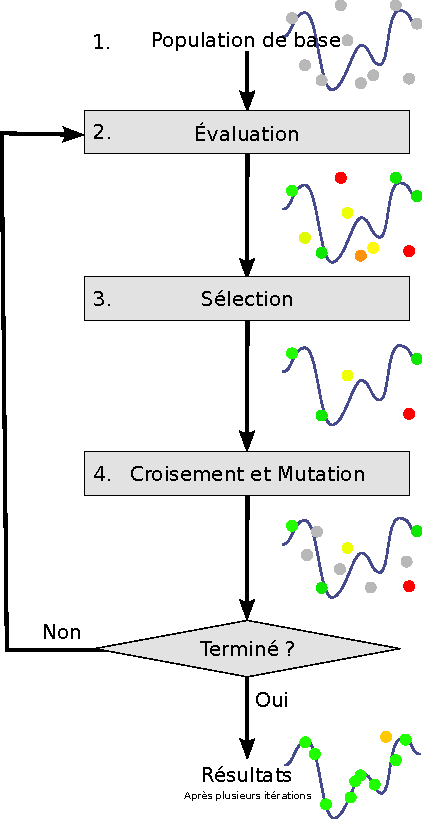
\includegraphics[width=.4\textwidth]{img/algo_genetique.pdf}
  \caption{Schéma des étapes d'un algorithme génétique}
  \label{cache:fig:genetic_schema}
\end{figure}

La Figure~\ref{cache:fig:genetic_schema} illustre le mécanisme de fonctionnement d'un algorithme génétique.

Un algorithme génétique démarre en utilisant une population d'individus de base qui est représentée dans l'étape 1 sur la Figure~\ref{cache:fig:genetic_schema}.
Dans le cas du \ac{RPCA}, la population initiale est générée en tirant un $c_u$ au hasard entre $\cmin$ et $\cmax$ afin d'éviter les solutions inadmissibles d'emblée.

Cette population va subir un traitement systématique pendant un nombre fini d'itérations appelées \emph{générations}.
Ce traitement est composé de plusieurs étapes: évaluation des aptitudes de chaque solution, sélection des meilleurs individus, croisement et application des mutations.
Ces étapes permettent de créer une nouvelle population et ce cycle recommence pendant un nombre fixé de générations ou bien lorsque les populations sont acceptables.
Les meilleures solutions qui ont été sélectionnées au fil des générations sont données comme solution au problème et constituent une approximation du front de Pareto.

\subsection{Aptitude}
\label{cache:fitness}

La fonction d'aptitude (ou ``fitness'' en anglais) évalue à quel point une solution est admissible ou non et si elle l'est quelle est son efficacité.
L'algorithme génétique n'impose aucune hypothèse sur cette fonction qui doit seulement renvoyer un réel.

Déterminer une fonction d'aptitude est la partie la plus liée au problème multi-objectifs lors de la conception d'un algorithme génétique; les autres étapes étant relativement génériques d'un problème à l'autre.

Pour chaque $\mathcal{C}$, il y a deux critères à prendre en compte: la durée de vie minimale du \ac{LLN} qu'il permet d'obtenir et la satisfaction que les utilisateurs auront si ce $\mathcal{C}$ est utilisé.
Soit $\mathcal{L}(\mathcal{C})$ la durée de vie obtenue dans le pire cas c'est-à-dire quand $r_u = c_u$.
Soit $\Gamma(\mathcal{C})$ qui est la satisfaction moyenne ressentie par l'utilisation et qui est définie comme: $\Gamma(\mathcal{C}) = \frac{1}{N}\sum_{u} \gamma_u$.

Soit $f$ la fonction d'aptitude obtenue en normalisant les grandeurs $\mathcal{S(C)}$ et $\mathcal{L(C)}$ entre $0$ et $1$:

\begin{align}
  f(\mathcal{C}) &= \frac{1}{2} \left(
    \frac{\Gamma(\mathcal{C}) - \Gamma(\mathcal{C}_{\textrm{min}})}
    {\Gamma(\mathcal{C}_{\textrm{max}}) - \Gamma(\mathcal{C}_{\textrm{min}})}
    +
    \frac{\mathcal{L(C)} - \mathcal{L(C_{\textrm{min}})}}
    {\mathcal{L(C_{\textrm{max}})} - \mathcal{L(C_{\textrm{min}})}}\right)
    \label{cache:eq:fitness1}\\
                 &= \frac{1}{2} \left(\Gamma(\mathcal{C})
      +\frac{\mathcal{L(C)} - \mathcal{L(C_{\textrm{min}})}}
      {\mathcal{L(C_{\textrm{max}})} - \mathcal{L(C_{\textrm{min}})}}\right)
  \label{cache:eq:fitness2}
\end{align}

Or, puisque $\Gamma(\mathcal{C}_{\textrm{min}}) = 0$ et $\Gamma(\mathcal{C}_{\textrm{max}}) = 1$,  l'équation~\eqref{cache:eq:fitness1} peut être simplifiée pour obtenir~\eqref{cache:eq:fitness2}.
D'autre part, la moyenne permet de ne pas privilégier des solutions conservatrices en énergie au détriment d'autres.

\subsection{Sélection}
\label{cache:selection}

Le processus de sélection utilise l'aptitude précédemment définie pour sélectionner les solutions qui vont se ``reproduire''.
Un des écueils courant des méthodes d'optimisation multi-objectifs génétique est de rester bloqué dans un sous-ensemble de solutions très homogènes.
Dans le cas du \ac{RPCA} cela voudrait dire que les solutions resteraient fixées sur un point localement optimal, or l'objectif est d'avoir une population aussi diversifiée que possible afin de pouvoir changer rapidement de solution en cas de changement de trafic.

Ainsi, à niveau d'aptitudes semblables, les solutions les plus éloignées les unes des autres devraient être sélectionnées.
C'est la méthode utilisée par NSGA-II~\cite{deb1999niched} qui est élitiste: les meilleures solutions sont retenues d'une génération à l'autre et forment les élites.
Cependant, cette sélection s'accompagne d'une préservation de la diversité qui privilégie les solutions éloignées les unes des autres.

Pour fonctionner, NSGA-II utilise une métrique d'estimation de densité qui va estimer la distance moyenne qui le sépare des autres solutions.
Puis lorsque deux solutions doivent être départagées lors d'une sélection, celle qui est la plus éloignée des autres solutions sera choisie.
Cette méthode de sélection permet d'avoir un large ensemble de solutions et sera celle utilisée pour le reste du chapitre.

D'autre part, cette méthode garde en mémoire les meilleures solutions vues à chaque génération (``hall of fame'' en anglais) afin de ne perdre aucune solution intéressante même si par le hasard des sélections elle n'est pas sélectionnée.

\subsection{Croisement \& Mutation}
\label{cache:mutation}

Les algorithmes génétiques utilisent des opérateurs afin d'altérer les populations de solutions existantes pour en former de nouvelles et explorer ainsi l'espace des solutions.
Il existe essentiellement deux opérateurs génétiques: le croisement et la mutation.

Comme de nombreuses méta-heuristiques, ces mécanismes très hétérogènes peuvent être complexes à configurer, car de nombreux paramètres sont disponibles.
Cependant, l'utilisation d'algorithmes de sélection élitiste permet de mitiger cette complexité, car les meilleures solutions sont gardées en mémoire dans le ``hall of fame''.
Ainsi, les mécanismes de mutation et de croisement peuvent être configurés pour être  ``exploratoire'', tandis que les mécanismes de sélection s'occupent de garder les meilleures solutions.

\subsubsection{Mutation}

La mutation est un processus de transformation qui est appliquée sur chaque individu avec une probabilité $p_m$ à chaque génération.
Ce processus modifie les gènes d'une solution (en l’occurrence les $c_u$) dans les bornes inférieures et supérieures admissibles (en l’occurrence $\cmin$ et $\cmax$).

Le reste de cette thèse utilise la méthode préconisée par les auteurs de NSGA-II qui est une mutation polynomiale qui utilise une distribution polynomiale définie entre $\cmin$ et $\cmax$~\cite{deb2014analysing}.

\subsubsection{Croisement}

Le croisement est un mécanisme d'exploration qui prend deux sous-ensembles de $c_u$, $c'_u$ appartenant à deux solutions distinctes $\mathcal{C}$ et $\mathcal{C}'$ et les échangent à la génération suivante.

\begin{figure}[ht]
  \centering
  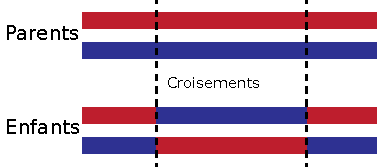
\includegraphics[scale=1]{img/crossover.pdf}
  \caption{Croisement de deux individus par points doubles}
  \label{cache:fig:crossover}
\end{figure}

La Figure~\ref{cache:fig:crossover} illustre ce mécanisme de croisement à point double qui sélectionne deux points et échange l'ensemble des gènes entre ces deux points.
C'est le mécanisme de croisement qui est recommandé pour être appliqué à NSGA-II ~\cite{Luke2013Metaheuristics} et qui sera utilisé dans cette thèse.

\section{Validation expérimentale}
\label{cache:validation}

Le \ac{RPCA} est évalué dans le scénario suivant: 12 serveurs \ac{CoAP} utilisant la bibliothèque Erbium~\cite{kovatsch2011low} sont déployés.
Ces nœuds utilisent Contiki~\cite{dunkels2004contiki} comme système d'exploitation et sont émulés via Cooja~\cite{cooja}.
Cooja les émule comme des TmoteSky fonctionnant avec un processeur de type MSP430 et utilisant pour communiquer une puce radio CC2420 dont les consommations énergétiques sont connues~\cite{Polastre05}.

\begin{figure}[ht]
  \centering
  \begin{tikzpicture}
  % définition des styles
  \tikzstyle{root}=[circle, draw, fill=red!50,text=black]
  \tikzstyle{node}=[circle, draw, fill=blue!50,text=black]

  \tikzstyle{estun}=[-,>=latex,very thick]
  % les nœuds
  \node[root] (root) at (0, 0) {root};

  \node[node] (1) at (1,0) {1};
  \node[node] (2) at (1,1) {2};
  \node[node] (3) at (0,1) {3};
  \node[node] (4) at (-1, 1) {4};
  \node[node] (5) at (-1, 0) {5};
  \node[node] (6) at (-1, -1) {6};
  \node[node] (7) at (0, -1) {7};
  \node[node] (8) at (1, -1) {8};

  \node[node] (9) at (2, 2) {9};
  \node[node] (10) at (-2, 2) {10};
  \node[node] (11) at (-2, -2) {11};
  \node[node] (12) at (2, -2) {12};

  \draw[estun] (root)--(1);
  \draw[estun] (root)--(3);
  \draw[estun] (root)--(5);
  \draw[estun] (root)--(7);

  \draw[estun] (1)--(2);
  \draw[estun] (2)--(3);
  \draw[estun] (3)--(4);
  \draw[estun] (4)--(5);
  \draw[estun] (5)--(6);
  \draw[estun] (6)--(7);
  \draw[estun] (7)--(8);
  \draw[estun] (8)--(1);

  \draw[estun] (2)--(9);
  \draw[estun] (4)--(10);
  \draw[estun] (6)--(11);
  \draw[estun] (8)--(12);

  \end{tikzpicture}

  \caption{Topologie radio considérée pour la validation expérimentale du \ac{RPCA}.}

  \label{cache:fig:topology}
\end{figure}

La Figure~\ref{cache:fig:topology} représente la topologie radio utilisée où un lien signifie que les nœuds peuvent être en communication radio l'un avec l'autre.
Les nœuds utilisent le protocole \ac{RPL}~\cite{rfc6550} pour établir une topologie de routage qui est connue par le routeur de bordure afin de modéliser la durée de vie du réseau.

\begin{table*}[ht]
\centering
\begin{tabular}{|l|c|c|}
\hline
Débit de transmission & $R$ & 250 kbps \\
\hline
Intervalle entre deux tentatives de préambules & $T_\pkt$ & 0.4 ms \\
\hline
Temps d'une période MAC & $T_\cycle$ & 0.244 s\\
\hline
Temps d'une période active & $T_\act$ & 40 ms\\
\hline
Temps pour détecter un paquet \ac{ACK} & $T_\detect$ & 0.16 ms \\
\hline
Taille d'une requête CoAP (\texttt{GET}) & $L_\req$ & 87 octets\\
\hline
Taille d'une réponse CoAP & $L_\ans$ & 96 octets \\
\hline
Temps pour transmettre un \ieee{} \ac{ACK} & $T_\ack$ & 0.608 ms  \\
\hline
Puissance consommée lors de la transmission & $P_\tx $ & 0.0511 W  \\
\hline
Puissance consommée lors de la réception & $P_\rx $ & 0.0588 W  \\
\hline
Puissance consommée lors du sommeil & $P_\sleep$ & $2.4\cdot 10^{-7}$ W \\
\hline
Nombre de nœuds dans le \ac{LLN}  & $N$ & 12 \\
\hline
Nombre de run par configuration &  & 10  \\
\hline
Nombre de requêtes \ac{CoAP} traité par nœuds &  & 50 \\
\hline
\end{tabular}
\caption{Paramètres utilisés dans les simulations.}

\label{cache:table:sim_parameters}
\end{table*}

Le tableau~\ref{cache:table:sim_parameters} donne les paramètres numériques utilisés lors de l'expérience.
Les nœuds utilisent ContikiMAC comme mécanisme de cycle de veille afin d'économiser de l'énergie et démarrent tous avec la même énergie initiale.
La consommation énergétique du réseau est obtenue en utilisant la topologie et la modélisation de ContikiMAC précédemment introduite.
La durée de vie du \ac{LLN} est calculée comme l'intervalle de temps entre son démarrage et la perte de son premier nœud.

Le \ac{RPCA} met en cache les réponses rendues par les nœuds afin de les mettre à disposition pour une éventuelle autre demande entrante.
Une fois la topologie et le trafic connus, la résolution du problème multi-objectif est lancée et les différents $\mathcal{C}$ sont calculés.
Le \ac{RPCA} a suffisamment de mémoire pour retenir toutes les réponses pour chaque \ac{URI} disponible dans le réseau.
La passerelle est toujours allumée, car non contrainte en énergie et assure une connexion permanente à un réseau local conventionnel.

Des requêtes \ac{HTTP} sont envoyées vers le \ac{RPCA} puis sont traduites vers une requête \ac{CoAP} et inversement en utilisant la bibliothèque Californium~\cite{kovatsch2014californium}.
Le trafic ne démarre que lorsque la topologie de routage est établie.

Le temps entre chaque requête est modélisé par un temps d'attente exponentiel de paramètre $\lambda_u$ et $\forall u, \lambda_u = \lambda$.
Ainsi le temps entre chaque requête correspond à $r_u$ pour le nœud qui héberge la ressource $u$.
Afin d'avoir une empreinte mémoire faible, chaque serveur n'a qu'une seule ressource et afin de faciliter l'analyse sera un texte de taille fixe ne causant pas de fragmentations.
Il est supposé que le trafic est suffisamment faible pour que les pertes de paquets soient négligeables.

\subsection{Compromis entre durée de vie et satisfaction utilisateur}

Le \ac{RPCA} est configuré pour utiliser un algorithme génétique pour trouver les solutions avec les paramètres suivants:

\begin{table*}[ht]
\centering
\begin{tabular}{|l|c|c|}
\hline
Population & $P$ & 100 \\
\hline
Probabilité d'accouplement & $p_c$ & 0.5 \\
\hline
Probabilité de mutation & $p_m$ & 0.2 \\
\hline
Nombre de générations & $n_g$ & 50 \\
% \hline
% Index de la distribution de mutation & $\eta_m$ & 20 \\
\hline
Temps de validité en cache minimal & $\cmin$ & 1s \\
\hline
Temps de validité en cache maximal & $\cmax$ & 9s \\
% \hline
% Taux de requêtes entrantes & $\lambda$ & 1 \\
\hline
\end{tabular}
\caption{Paramètres utilisés dans l'optimisation multi-objectifs.}

\label{cache:table:nsga2_parameters}
\end{table*}

\begin{figure}[ht]
  \centering

 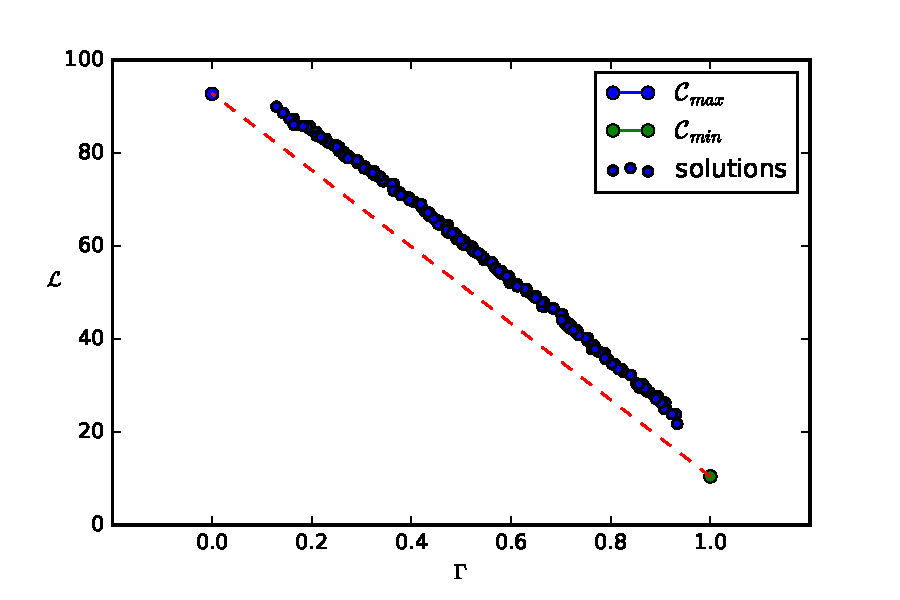
\includegraphics[width=.7\textwidth]{img/pareto.pdf}

 \caption{Front de Pareto pour le scénario envisagé.}

 \label{cache:fig:paretofront}

\end{figure}

Les probabilités d'accouplement et de mutation sont laissées aux valeurs recommandées par les créateurs de NSGA-II.
Le nombre de générations et la taille de population sont choisis afin d'avoir un temps de calcul modeste et d'obtenir une approximation du front de Pareto rapide.
La Figure~\ref{cache:fig:paretofront} montre la population de solutions produites par l'algorithme génétique.
Chaque point solution est un $\mathcal{C}$ contenant l'ensemble des $c_u$.
Ces points forment une approximation du front de Pareto qui représente les solutions optimales et les durées de vie mesurées en jours.

Les poins $\mathcal{C}_{min}$ et $\mathcal{C}_{max}$ sont également présentés afin de montrer les bornes possibles des solutions.
Ainsi si  $\mathcal{C}_{min}$ garantie une fraîcheur aussi élevée que possible, mais raccourcit la durée de vie alors que $\mathcal{C}_{max}$ garantie une durée de vie aussi longue que possible.

Une valeur haute de $c_u$ sera utilisée pour des nœuds ayant peu d'énergie.
Par contre, une valeur $c_u$ petite sera pour des informations devant être aussi récentes que possible.

\subsection{Cache hit}

\begin{figure}[ht]
  \centering
  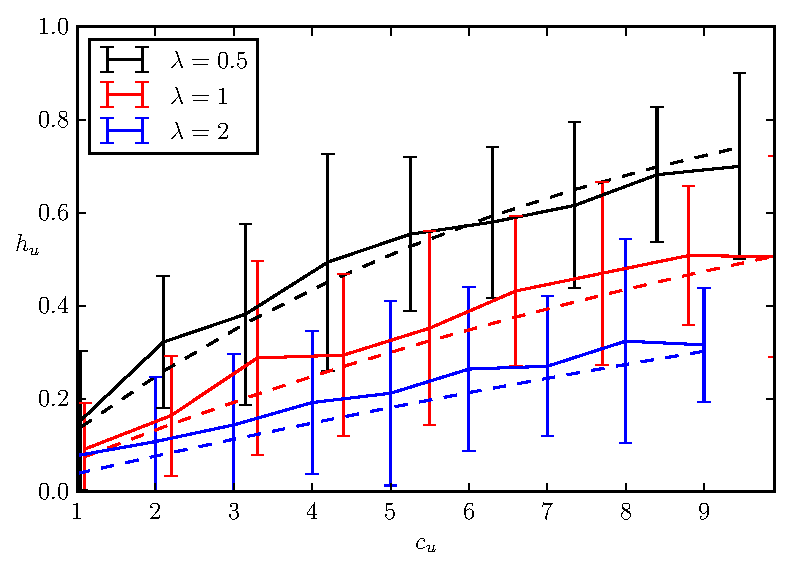
\includegraphics[width=.5\textwidth]{img/new_cachinghit.pdf}
  \caption{Évolution du cache hit en fonction de la durée de vie}
  \label{cache:fig:hit}
\end{figure}

La Figure~\ref{cache:fig:hit} illustre l'évolution du nombre de requêtes servies par le cache (hit) en fonction de la durée de vie des requêtes $c_u$ choisies.
La simulation (traits pleins) est comparée à la modélisation théorique (lignes en pointillés cf~\eqref{cache:eq:cache_hit}) pour différentes valeurs de paramètres $\lambda$ sur la Figure~\ref{cache:fig:hit}.
Afin de simplifier la représentation visuelle, le graphique montre quels sont les résultats obtenus lorsque tous les $c_u$ et $\lambda_u$ sont égaux entre eux.

Plus $c_u$ est grand par rapport à $T_u = \frac{1}{\lambda_u}$, plus le cache est efficace, car la probabilité que la requête soit servie par le \ac{RPCA} augmente épargnant ainsi aux nœuds du \ac{LLN} de les traiter.

Quand $c_u$ est petit devant $T_u = \frac{1}{\lambda_u}$, la fréquence de requête est plus faible que le temps de vie dans le cache.
Le cache est ici inefficace, car une réponse n'y vit pas assez longtemps pour être susceptible d'être utilisée.

Ainsi l'efficacité d'un cache n'est pas seulement liée au temps de vie d'une requête, mais également à son adéquation avec le trafic qu'il reçoit.

\subsection{Amélioration de la durée de vie}

\begin{figure}[ht]
  \centering
  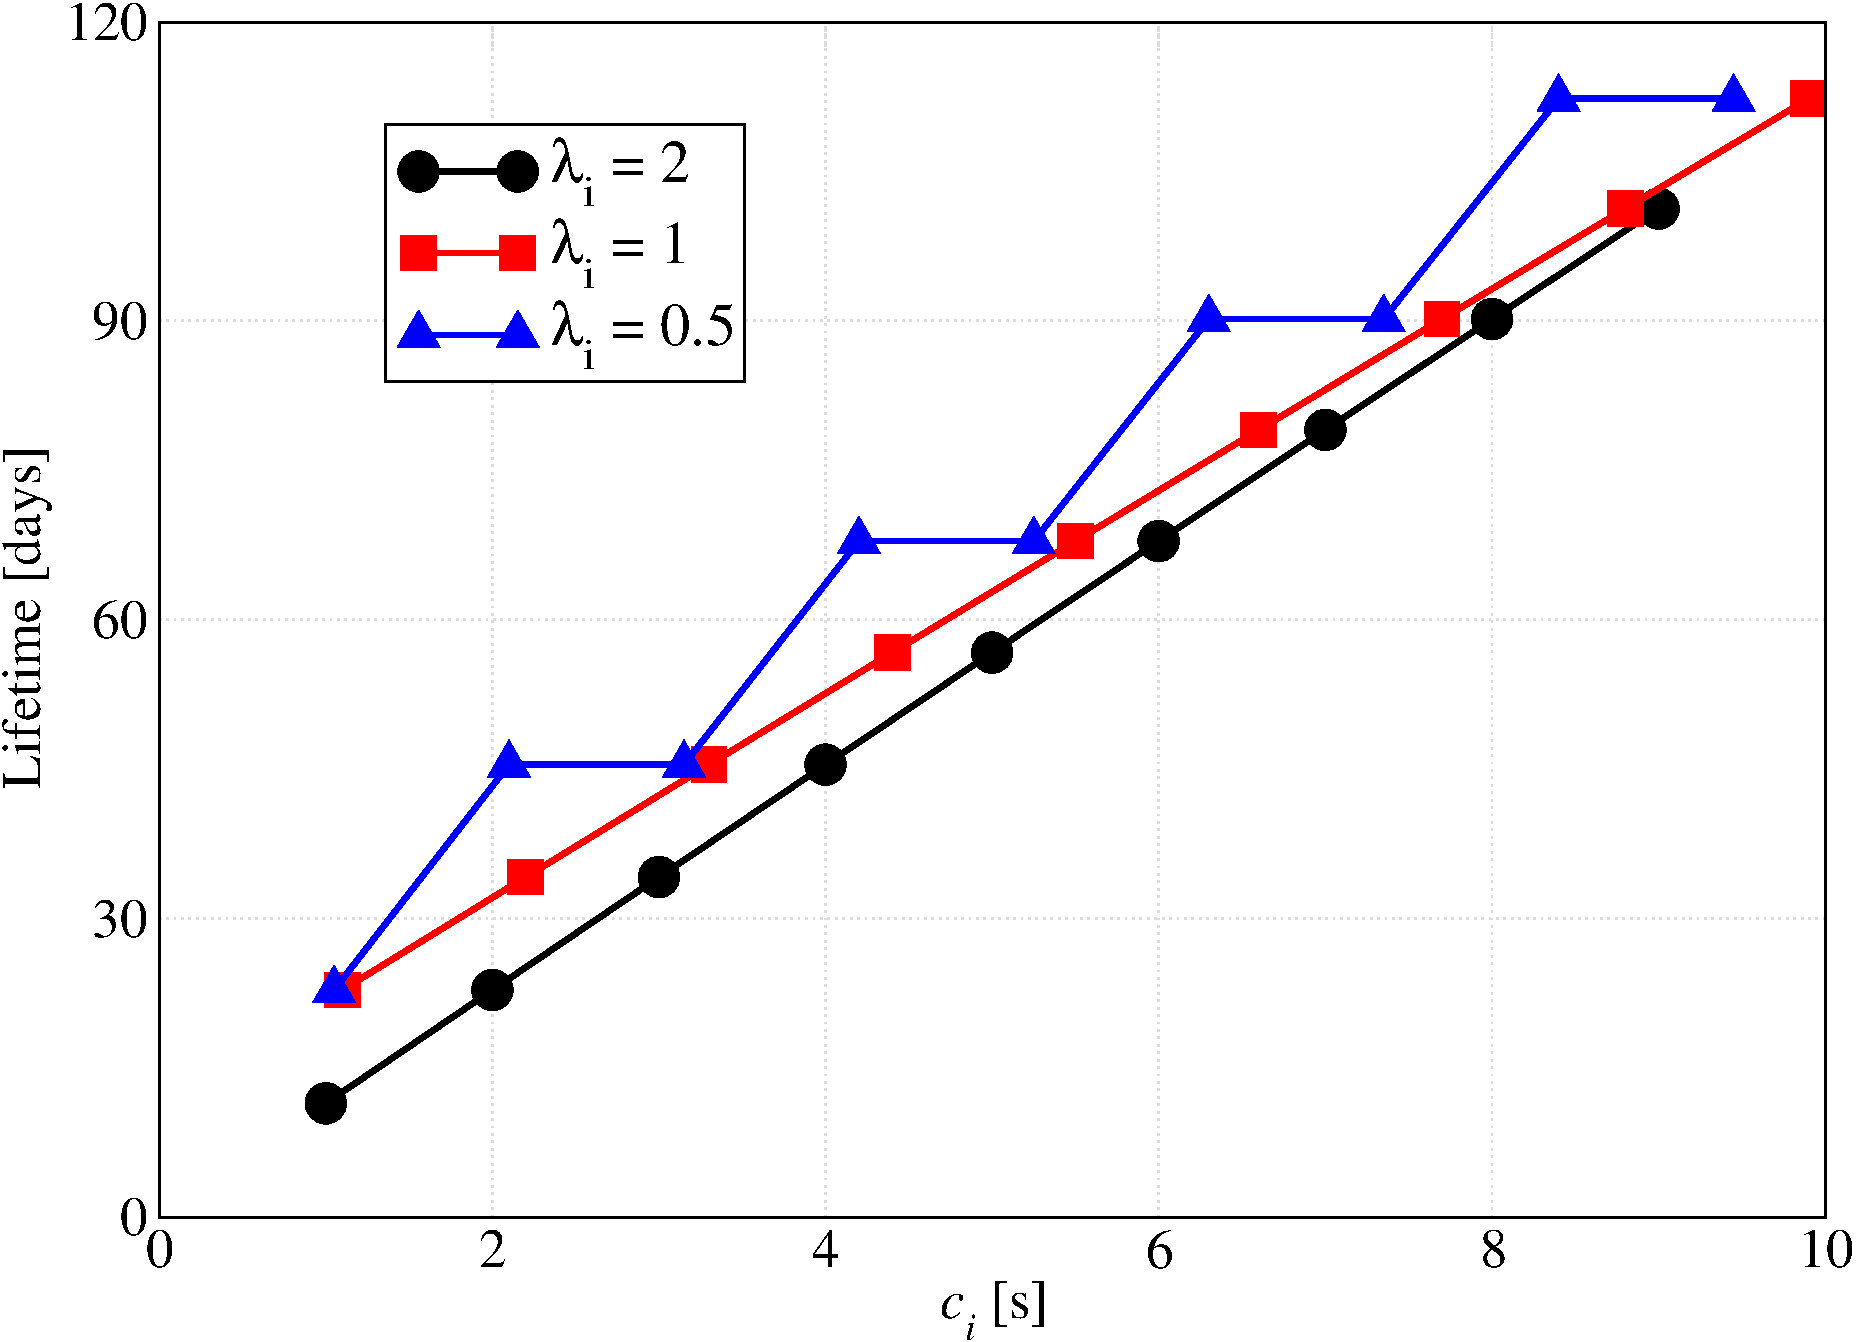
\includegraphics[width=0.455\textwidth]{img/lifetime.pdf}
  \caption{Évolution de la durée de vie théorique en fonction des $c_u$}
  \label{cache:fig:lifetime}
\end{figure}

La Figure~\ref{cache:fig:lifetime} illustre la durée de vie théorique obtenue pour le \ac{LLN} pour différentes configurations de cache identiques.
Il est observé que plus les temps de cache sont élevés, plus la durée de vie du \ac{LLN} est élevée ce qui est attendu, car une grande durée de vie implique que moins de requêtes applicatives sont gérées par le \ac{LLN}.

\section{Conclusion}
\label{cache:conclusion}

% Résumé

Ce chapitre montre comment un \ac{RPCA} permet d'optimiser l'utilisation des ressources d'un \ac{LLN} en adaptant la quantité de requêtes applicatives admises dans le \ac{LLN}.
Ce mécanisme utilise une modélisation de la consommation énergétique et de la satisfaction des utilisateurs afin de fournir un temps de vie pour toutes les réponses
aux requêtes que le \ac{RPCA} doit gérer.

% Avantages

Un \ac{RPCA} change dynamiquement la quantité de requêtes applicatives entrantes dans un \ac{LLN} afin d'économiser ses ressources d'une part et d'accélérer le traitement des requêtes d'autre part.
De plus, le \ac{RPCA} utilise une estimation de la durée de vie pour aider l'administrateur d'un \ac{LLN} à trouver une configuration adaptée pour les objectifs de durée de vie visés.

% Limitations

L'utilisation d'algorithme génétique permet d'avoir un mécanisme général pouvant être appliqué à n'importe quelle situation.
Cependant, cette méthode n'offre pas de garanties de convergence vers le front de Pareto pour un nombre de générations donné.
Des méthodes plus spécifiques utilisant notamment une hypothèse de convexité sur les fonctions objectifs permettrait d'aller plus vite.

% Amélioration

Une piste d'amélioration possible consisterait à tester d'autres méthodes de résolutions d'optimisations multi-objectifs afin de comparer avec d'autres mécanismes présentant la même flexibilité.
Cependant, la tâche est complexe, car le nombre d'heuristiques disponibles dans la littérature est très élevé et implémenter ces heuristiques est long et met en jeu de nombreux paramètres de configuration rendant cette exploration difficile.

Une autre amélioration peut également être envisagée pour fournir un modèle de satisfaction des utilisateurs prenant en compte le nombre de requêtes reçues.
Ainsi, le \ac{RPCA} pourrait utiliser une modélisation de la satisfaction des utilisateurs tenant compte des popularités respectives des différentes \ac{URI}.

Enfin, un \ac{RPCA} pourrait également être étendu afin de gérer la fréquence d'envois des observations en provenance des nœuds.
Dans certains \ac{LLN}s, les nœuds envoient périodiquement des notifications à la passerelle afin qu'elle puisse redistribuer cette notification aux abonnés intéressés.
N'avoir que la passerelle comme abonné allège la charge qu'un nœud doit gérer.
Le \ac{RPCA} pourrait configurer les nœuds pour réguler la fréquence d'envoi des notifications.
L'objectif serait de trouver le bon compromis entre la satisfaction des utilisateurs qui veulent des informations régulièrement et les nœuds qui veulent envoyer aussi peu de notifications que possible.

\section*{Publications}

\begin{itemize}
  \item Rémy Leone, Paolo Medagliani et Jérémie Leguay.
    \newblock {Optimizing QoS in Wireless Sensors Networks using a Caching Platform}.
    \newblock {\em {Sensornets 2013}}, page~56, Barcelone, Espagne, Février 2013.

  \item Rémy Leone, Paolo Medagliani et Jérémie Leguay.
    \newblock {Optimisation de la qualité de service par l'utilisation de mémoire cache}
    \newblock 15{\`e}mes Rencontres Francophones sur les Aspects Algorithmiques des T{\'e}l{\'e}communications

\end{itemize}
% !TEX root = ../main.tex
% !TeX spellcheck = fr_FR

\chapter{Expériences automatisées et reproductibles pour \ac{LLN}s} 
\label{makesense}

% \epigraph{It doesn't matter how beautiful your theory is, it doesn't matter how smart you are. 
% If it doesn't agree with experiment, it's wrong.}{Richard Feynman}

\epigraph{Besides black art, there is only automation and mechanization.}{Federico Garcia Lorca}

\minitoc

% Bien qu'étant une contribution importante, le contenu de ce chapitre n'est pas indispensable à la compréhension de la suite de cette thèse.
% Le lecteur désirant se concentrer sur les contributions relatives à la passerelle sans s'attarder sur la méthodologie des expériences pourra passer directement au chapitre suivant.
Ce chapitre présente Makesense, un framework permettant d'obtenir des expériences reproductibles, documentées et automatisables visant les \ac{LLN}s.
L'organisation du chapitre est la suivante:

La section~\ref{makesense:reproductibility} présente la reproductibilité d'expérience et la met en perspective avec la recherche sur les \ac{LLN}s.

La section~\ref{makesense:related} présente comment la documentation et l'automatisation sont faites dans l'état de l'art, comment l'interaction avec les nœuds physiques d'une plateforme est classiquement faite et les limites de chacune de ces approches.

La section~\ref{makesense:makesense} présente Makesense et les choix techniques effectués pour l'utiliser efficacement dans le contexte des \ac{LLN}s.

La section~\ref{makesense:conclusion} conclut ce chapitre en justifiant l'intérêt d'un tel framework pour la communauté scientifique.

\section{Introduction à la recherche reproductible dans les \ac{LLN}s}
\label{makesense:reproductibility}

\subsection{Reproductibilité}

Une expérience est définie comme une série d'actions ayant pour but de tester (confirmer ou infirmer) une hypothèse~\cite{fisher1960design,bachelard1975nouvel}.
Il y a trois éléments impliqués dans ce processus: le \emph{laboratoire} qui correspond à l'environnement (conditions, scénarios, etc.) dans lequel l'expérience se produit, l'\emph{expérimentateur} qui est la personne qui va faire l'expérience et le \emph{dispositif} qui est étudié. 
Si une expérience peut être exécutée dans des laboratoires avec des expérimentateurs et des dispositifs tous différents, mais arriver aux mêmes conclusions alors l'expérience est dite reproductible.

Dans le cas des \ac{LLN}s, une expérience peut consister à tester qu'un système (par exemple un cache) diminue le trafic qu'un \ac{LLN} doit gérer.
Dans ce cas, le laboratoire est l'endroit où cette expérience se produit, l'expérimentateur est l'agent humain ou automatisé effectuant l'expérience et le dispositif est le \ac{LLN} (simulé, émulé ou réel) étudié.

Construire une expérience reproductible est à la base de la méthode scientifique.
Pourtant mettre en place un environnement permettant de construire des expériences reproductibles est souvent perçu comme long et fastidieux.
De plus, la reproductibilité est peu valorisée à court terme aussi bien au moment de juger un article pour le publier dans une revue qu'après sa publication~\cite{fink2013conducting,wilson2014best} et cela malgré son importance fondamentale~\cite{popper-scientificdiscovery}.
Ce paradoxe a été relevé à de nombreuses reprises dans d'autres sciences et existe aussi en informatique \cite{peng2011reproducible}.

Des dépôts de documents scientifiques rendent aujourd'hui possible l'hébergement des fichiers nécessaires au déroulement d'une expérience en plus de la publication en elle-même.
Ainsi réduire la difficulté de mise en place d'expériences reproductibles est le verrou technique principal pour permettre sa diffusion et sa démocratisation.

\subsection{Problématiques expérimentales des \ac{LLN}s} 

Développer une expérience pour \ac{LLN} peut être complexe en raison de la grande hétérogénéité des technologies mises en jeu (systèmes embarqués, transmissions de messages sur réseau, analyse de résultats)~\cite{baronti2007wireless}.
Ainsi des compromis doivent être trouvés entre le degré de réalisme souhaité et le temps de développement nécessaire pour mettre en place une expérience afin d'avoir des résultats pertinents au plus tôt.

\begin{figure}[ht]
\begin{tikzpicture}[->,>=latex,shorten >=1pt,auto,node distance=3cm,
  thick,main node/.style={fill=blue!20,draw}]

  \node[main node] (sim) at (0,0) {\begin{tabular}{c}Simulation\end{tabular}};
  \node[main node] (emu) at (4,0) {\begin{tabular}{c}Emulation\end{tabular}};
  \node[main node] (iotlab) at (8,0) {\begin{tabular}{c}Testbed\end{tabular}};
  \node[main node] (final) at (12,0) {\begin{tabular}{c}Déploiement\end{tabular}};

  \path
    (sim) edge[] (emu)
    % (emu) edge [bend left=10] node[below] {Modèle} (sim)

    (emu) edge[] (iotlab)
    % (iotlab) edge [bend left=10] node[below] {Prototype} (emu)

    (iotlab) edge[] (final)
    % (final) edge [bend left=10] node[below] {Finalisation} (iotlab)

;
\end{tikzpicture}
\caption{Évolution d'une expérience vers le réalisme}
\label{makesense:fig:workflow}
\end{figure}

La Figure~\ref{makesense:fig:workflow} illustre les différents choix de niveaux d'abstraction de développement pour une expérience portant sur les \ac{LLN}s.
Il existe essentiellement 4 niveaux d'abstraction différents chacun ayant un différent compromis entre réalisme et facilité de développement.

Les simulateurs et émulateurs n'utilisent pas des nœuds physiques et permettent d'avoir dans un programme un fonctionnement modélisé d'un \ac{LLN} afin d'illustrer son fonctionnement aussi rapidement que possible.

Vérifier des résultats de simulations sur des nœuds physiques apporte une confirmation aux résultats trouvés en simulation.
Cependant effectuer des expériences sur un grand nombre de nœuds requiert de disposer physiquement de ces nœuds.
Il peut être coûteux pour un laboratoire d'investir pour acheter, mettre en place et maintenir tous les nœuds requis pour une expérience donnée.
Ainsi des plateformes publiques (``testbeds'' en anglais) sont apparues afin de mutualiser un grand nombre de nœuds physiques entre plusieurs équipes de recherche~\cite{doddavenkatappa2012indriya, fleury2015fit}.
Ces plateformes mettent à la disposition de leurs utilisateurs des nœuds physiques avec des architectures matérielles variées sur lesquels un utilisateur déploie son système.
Elles offrent des traces détaillées de l'expérience et permettent de déployer sur des nœuds représentatifs d'un capteur un code spécifique et de mesurer l'évolution de ce nœud au cours du temps~\cite{fleury2015fit}.

Les sous-sections suivantes exposent plus en détail les différents compromis de chaque niveau et la difficulté de porter les développements faits à un niveau donné vers un niveau plus réaliste.

\subsubsection{Expérience sur simulateur}
\label{makesense:simulation}

Un simulateur permet d'avoir une modélisation du \ac{LLN} sous la forme d'un programme qui une fois exécuté renvoie des résultats~\cite{sobeih2006j,abdeddaim2011implementation}.

L'atout d'un simulateur réside dans son environnement qui est totalement contrôlé, détaillé et sur la capacité de simuler des scénarios avec un grand nombre de nœuds sur des temps longs avec des temps courts de simulation~\cite{jevtic2009evaluation}.
Si les graines des générateurs de nombres aléatoires sont fixées, alors on a une reproductibilité complète de l'expérience si on ré-exécute le même programme avec les mêmes entrées deux fois de suite.
En outre, le simulateur étant un système isolé, corriger le système et tester une nouvelle idée est relativement facile.

Cependant, les simulateurs font un certain nombre d'approximations sur le médium de transmission et plus généralement sur le fonctionnement des nœuds, la dérive des horloges, l'usure des composants et les pannes éventuelles.
Ainsi les simulations ne correspondent pas fidèlement à un déploiement sur nœuds réels et des problèmes non prévus peuvent subvenir lorsqu'un déploiement réel se produit.

\subsubsection{Expérience sur émulateur}
\label{makesense:emulation}

Un émulateur permet de substituer une architecture matérielle physique par un logiciel.
Les émulateurs sont activement utilisés afin de permettre un développement logiciel rapide qui ne nécessite pas d'installer un code sur un nœud physique à chaque changement~\cite{cooja}.

Ainsi dans le cas d'une simulation, au lieu d'utiliser un programme ad hoc le simulateur utilise un émulateur d'architecture matérielle afin de disposer d'informations plus réalistes sur le fonctionnement d'un nœud comme des visualisations du cycle de veille des nœuds, de la consommation énergétique estimée de chaque nœud et de pouvoir inspecter le code s’exécutant sur un nœud durant une simulation.
Émuler permet de tester un code réel, tandis que simuler oblige à utiliser une abstraction du code exécuté.

Cependant, un émulateur est soumis aux mêmes limitations qu'un simulateur, toutes les interactions (transmission, dérive d'horloge) sont modélisées par des logiciels et sont donc d'un réalisme limité.

\subsubsection{Expérience sur plateforme}
\label{makesense:testbeds}

L'objectif des déploiements sur plateforme est de fournir des nœuds physiques réels aux expérimentateurs afin d'exécuter des expériences dans des conditions plus réalistes que celle d'un simulateur ou d'un émulateur.

L'utilisation des plateformes est répandue en recherche et de nombreux travaux s'appuient sur ces plateformes pour effectuer des expériences~\cite{handziski2006twist}.

Cependant, effectuer une expérience sur plateforme présente des différences de fond par rapport aux expériences sur simulateur et émulateur.
Le temps ne pouvant être accéléré comme sur un simulateur, des expériences longues sont nécessaires pour tester la fiabilité sur de grandes périodes de temps.
Puisque les nœuds sont réels, ils peuvent tomber en panne et avoir des avaries, ainsi, il est impossible de garantir de manière systématique et déterministe, que deux expériences donneront exactement les mêmes résultats. 

Dans le cas de plateformes mutualisées et distantes, il est nécessaire de partager les réservations des nœuds ainsi que de communiquer avec cette plateforme via des interfaces spécifiques ce qui rajoute un niveau de complexité à l'expérience.
Enfin, les déploiements sur ces plateformes se font le plus souvent sur des nœuds à l'intérieur de bâtiment, statiques dans l'espace, dans des environnements contrôlés et offrant peu de variabilité.
Ainsi, il n'est pas toujours possible de contrôler l'environnement radio, la position des nœuds et l'atténuation des signaux entre les différents nœuds. 

\subsubsection{Expérience en déploiement réel}
\label{makesense:real_deployment}

Déployer une expérience sur nœuds réels permet d'avoir un système dans des conditions aussi réalistes et proches que possible que celles dites de ``production'' d'un système finalisé.

Le réalisme dans ce cas est très proche des conditions réelles d'un \ac{LLN} déployé dans son environnement cible.
Cette phase qui est généralement faite en phase de finalisation est plus coûteuse car il faut disposer des nœuds physiques, les installer dans une zone potentiellement large et subir les conditions logistiques de déploiement~\cite{werner2006deploying}.
Dans ces conditions, modifier les nœuds peut être complexe si l'environnement est hostile ou si les nœuds ne peuvent pas être mis à jour facilement à distance.

\subsubsection{Transitions entre niveaux}
\label{makesense:transition}

L'objectif d'une expérience est de se rapprocher autant que possible de la réalité afin de permettre de modéliser des problèmes et d'y apporter des solutions.
Cette progression vers le réalisme peut être accélérée par la réutilisation des systèmes développés lors d'étapes préalables.

Passer de l'étape de simulation à l'émulation permet de gagner en réalisme et de modéliser plus finement un \ac{LLN} car une partie des contraintes mémoires des architectures matérielles des nœuds sont prises en compte grâce à l'émulateur.
L'analyse des données et leur visualisation peuvent être conservées, car une partie des sorties de l'expérience (par exemple les logs séries) peuvent être au même format et analysées de la même façon.

Le passage de l'émulation à la plateforme permet de gagner en réalisme, car les contraintes des nœuds physiques apparaissent.
Les images binaires produites lors du prototypage avec un émulateur peuvent être conservées, ainsi il n'est pas nécessaire de les réécrire.
De plus, le code écrit pour analyser les résultats peut être également conservé, car les sorties séries peuvent être au même format.

Enfin, le passage de la plateforme au déploiement réel met en jeu des contraintes qui sont spécifiques à un déploiement donné et à sa finalisation, ainsi cette difficulté souvent logistique ne peut être évitée et dépend de chaque contexte.
Cependant, le binaire faisant fonctionner les nœuds et l'analyse des résultats conçus précédemment peuvent être conservés.

On peut observer que la progression vers le réalisme est un processus itératif et qu'une partie des développements peuvent être conservés d'un niveau à l'autre afin d'économiser les coûts de mise en place.
Ainsi un framework permettant de documenter, d'automatiser et de réutiliser autant de fonctionnalités que possible entre les différents niveaux permet aux utilisateurs de se concentrer sur les verrous technologiques propres à chaque niveau au lieu de ré-implémenter l'ensemble de leur développement à chaque fois. 

\section{État de l'art sur les outils de gestion d'expériences}
\label{makesense:related}

Gérer une expérience sur des nœuds physiques ou émulés met en jeu de nombreuses étapes comme la préparation des nœuds, l'exécution et le traitement des données.
L'intégration de toutes ces étapes est longue et fastidieuse, ainsi il est nécessaire de la documenter et lorsque cela est possible de l'automatiser. 

\subsection{Documentation}

Les logiciels et plateformes utilisés par les \ac{LLN}s sont relativement nouveaux, ainsi, il est particulièrement important que leur documentation soit aussi claire et tenue à jour que possible afin de diffuser efficacement leur usage.
Cette documentation est actuellement essentiellement fournie par des didacticiels ad hoc et des wikis qui sont édités par la communauté des utilisateurs.
C'est notamment le cas des plateformes Indriya et FIT-IoT-lab~\cite{fleury2015fit,doddavenkatappa2011indriya} et des systèmes d'exploitation usuels tels que Contiki~\cite{dunkels2004contiki}, OpenWSN~\cite{watteyne2012openwsn} ou encore RIOT~\cite{baccelli2013riot}.
Cette approche est choisie, car elle est facile à mettre en place et permet de rapidement partager une expérience avec les utilisateurs, mais a le défaut de pouvoir devenir obsolète si elle n'est pas tenue à jour.

Une autre approche consiste à documenter un projet de manière systématique par l'utilisation d'un logiciel de documentation comme Doxygen~\cite{van2004doxygen} ou Sphinx~\cite{brandl2010sphinx}.
Cependant cette approche repose sur une idée de projet unique et cohérent, or les expériences sur les \ac{LLN}s mettent en jeu de très nombreux sous-projets hétérogènes dans des langages parfois différents rendant cette approche peu efficace.

Enfin, une approche alternative à la documentation consiste à intégrer du code exécutable dans le même document qui est utilisé pour décrire une expérience.
Ces documents enrichis sont souvent désignés par le terme de \emph{notebook} et sont couramment utilisés dans certaines communautés scientifiques et pédagogiques~\cite{young2003science,shen2014interactive}.
Cependant l'utilisation de ces notebooks est encore restreinte dans la communauté de recherche sur les \ac{LLN}s.

\subsection{Automatisation}
\label{makesense:related_automatisation}

Automatiser une expérience permet de la rendre reproductible, documentée et de la partager plus facilement, car toutes les étapes requises sont décrites dans le programme qui l'automatise~\cite{lee1992tools, king2009automation}.
De plus, l'automatisation d'un système permet de fournir des résultats cohérents d'une exécution d'expérience à l'autre et d'accélérer la prise en main d'un débutant, car toutes les étapes requises sont spécifiées.
En outre, corriger une erreur dans un procédé automatisé permet de l'éviter définitivement alors qu'une correction manuelle appliquée de manière ad hoc doit être effectuée de nouveau lorsque le contexte de l'expérience change.

Afin de décrire les dépendances entre les différentes étapes de l'expérience~\footnote{Par exemple: compiler les nœuds avant de les émuler.}, des outils génériques tels que \texttt{make} sont généralement utilisés pour garantir que les dépendances d'une étape donnée de l'expérience sont à jour~\cite{feldman1979make}.
Cependant, les vérifications préalables au lancement des étapes telles que les dépendances logicielles et matérielles sont rarement documentées ou testées lors de leur automatisation.
Or, ne pas tenir compte de ces différentes dépendances peut provoquer des erreurs subtiles à détecter notamment dans des logiciels en développement actif comme les systèmes d'exploitation des nœuds capteurs d'un \ac{LLN}.

\subsection{Déploiement d'expérience sur nœuds réels}

Un testbed met en jeu de multiples ressources pour des utilisateurs multiples, ainsi la gestion des ressources disponibles et leur réservation est une question fondamentale pour ces plateformes.
L'interface avec les testbeds est une question étudiée et de nombreux outils sont disponibles dans l'état de l'art pour s'interfacer avec eux aussi efficacement que possible~\cite{buchert2015survey}. 
Certains testbeds utilisent des frameworks spécifiques comme \ac{OMF} et son langage de description d'expériences \ac{OEDL} qui peuvent être utilisés pour décrire une expérience et déclencher des actions en fonction d’événements~\cite{rakotoarivelo2010omf}.
Cependant cette approche est coûteuse en temps, car elle requiert d'apprendre un \ac{DSL} qui repose sur un formalisme fixe et qui ne peut pas être réutilisé dans d'autres contextes.
Ainsi des approches plus génériques et indépendantes d'un langage donné sont plus adaptées pour favoriser la diffusion d'une expérience par exemple par l'utilisation d'une \ac{API}.

De plus, les frameworks permettant d'utiliser des testbeds disponibles dans la littérature ne proposent des abstractions que pour la réservation et le lancement d'expériences~\cite{auge2014tools,baron2012towards}.
Les interfaces proposées ne gèrent pas par exemple les processus et leur relance qui doivent être gérés par l'utilisateur.
Ainsi il est nécessaire pour un utilisateur de surveiller l'évolution d'une expérience pour réagir aux pannes éventuelles.
De plus, pour un utilisateur débutant, les multiples erreurs pouvant survenir sont parfois difficiles à interpréter quand peu d'informations sont disponibles pour aider.

\subsection*{Conclusion intermédiaire}

Comme vu dans cette section, l'état de l'art offre des solutions pour chacun des problèmes individuellement cependant leur intégration au sein d'un seul framework cohérent est encore manquant.

Les descriptions de protocoles expérimentaux peuvent être enrichies via un mécanisme de notebook pour fournir à la fois une description et du code au sein d'un même fichier.

L'automatisation est nécessaire pour garantir la consistance et la rapidité de mise en place, mais doit être couplée à la vérification des dépendances et intégrée avec la documentation afin de garantir que le code d'une expérience est exécuté dans un contexte défini et que toutes les dépendances sont satisfaites.

Enfin, l'utilisation des testbeds est utile pour avoir des expériences sur nœuds physiques et il faut privilégier leur intégration au sein de mécanismes généraux comme des \ac{API} afin d'éviter des \ac{DSL} qui forcent l'utilisation d'un formalisme spécifique.

\section{Makesense}
\label{makesense:makesense}

Makesense est un framework produit dans le cadre de cette thèse permettant d'obtenir la \emph{documentation}, l'\emph{automatisation} et la \emph{reproductibilité} d'une expérience.
Ce framework vise à réduire le temps nécessaire pour mettre en place une expérience reproductible en intégrant les différentes étapes d'une expérience dans un seul document enrichi afin d'exécuter une expérience aussi bien sur des nœuds simulés, émulés ou réels.
Makesense intègre plusieurs outils afin d'aboutir à cet objectif.

\paragraph{Utilisation d'un notebook pour contenir la documentation et le code d'une expérience}

Makesense utilise un notebook pour contenir à la fois la documentation d'une expérience et le code permettant de l'exécuter.
L'apport de fond d'un notebook se situe dans la juxtaposition de la documentation enrichie et du contexte d'exécution commun à l'ensemble du notebook.
La description d'une expérience dans un notebook est présentée de la même façon que dans un didacticiel, des étapes se suivent dans un ordre précis pour aboutir à un résultat.
Chaque étape peut être rejouée indépendamment, ainsi le coût pour rejouer une étape se limite a l'étape elle-même et pas à ses dépendances qui sont gardées en mémoire.

\paragraph{Utilisation d'un langage et d'un contexte communs}

Utiliser des outils hétérogènes et incapables de communiquer efficacement entre eux augmente la charge de développement et le temps requis pour intégrer ces différents composants~\cite{stanisic2015effective}.
Ainsi Makesense utilise un seul langage et partage un contexte d'exécution entre toutes les étapes afin de simplifier la compréhension d'une expérience et le partage des données.

\paragraph{Utilisation d'outils généraux et communs à plusieurs champs de recherche}

Développer un outil spécifique aux \ac{LLN}s limiterait d'emblée sa portée.
En outre, les processus de gestion d'expériences ont de nombreuses similarités avec des approches génériques de développement logiciel.
Makesense utilise des bibliothèques logicielles scientifiques et généralistes largement diffusées pour effectuer une expérience.
Ce choix permet d'éviter l'obsolescence des dépendances, car elles reposent sur des communautés actives et visent à offrir un pont entre les communautés scientifiques et celles liées au développement logiciel.

\paragraph{Approvisionnement d'expérience par l'utilisation de gabarits}

Les expériences sur les \ac{LLN}s mettent en jeu de nombreux fichiers (code source des nœuds, configuration d'un simulateur, etc.) qui peuvent être réutilisables d'une expérience à l'autre, notamment dans les cas de campagnes d'expériences.
Makesense génère ces fichiers de manière expressive en utilisant des gabarits de fichiers pour générer dynamiquement l'ensemble des fichiers nécessaires à une expérience donnée.
Ainsi une campagne d'expérience composée d'expériences paramétrables peut être conçue rapidement à partir des gabarits et des paramètres spécifiques de cette expérience.

\paragraph{Réutilisation des processus d'exploitation sur différents niveaux d'abstraction}

Une expérience, qu'elle se passe sur nœuds simulés, émulés ou physiques, conserve d'un niveau d'abstraction à l'autre des processus et des fonctions communes (par exemple l'analyse des données et leur mise en forme).

Makesense permet de documenter et d'automatiser ces processus communs afin de pouvoir les réutiliser autant que faire se peut d'un niveau d'abstraction à l'autre.
Ainsi les transitions entre les différents niveaux sont plus rapides, car les traitements communs sont conservés et peuvent être appliqués en séquence.

\paragraph{Utilisation d'outils de gestion de révisions et d'intégration continue}

Une expérience évolue au cours du temps, ainsi il est essentiel de garder en mémoire son évolution et de tester en permanence que les révisions apportées ne cassent pas les résultats précédemment obtenus et que les dépendances sont satisfaites.
Ainsi Makesense utilise un gestionnaire de révision et un service d'intégration continue afin de conserver toute l'évolution du développement d'une expérience et garantir que chaque nouvelle révision d'une expérience n'introduit pas d'erreurs.

\paragraph{Licence et démonstration}

Afin de favoriser son utilisation, Makesense est disponible sous licence Apache sur Github~\footnote{\href{https://github.com/sieben/makesense}{https://github.com/sieben/makesense}} et une démonstration du déroulement d'une expérience est également disponible~\footnote{\href{https://travis-ci.org/sieben/makesense}{https://travis-ci.org/sieben/makesense}}.

\subsection{Présentation d'une expérience typique sur les \ac{LLN}s}

Une expérience portant sur un \ac{LLN} commence le plus souvent par la génération des différents composants nécessaires à sa mise en place: binaire faisant fonctionner les nœuds, préparation et configuration des outils annexes (émulateurs, simulateurs, etc.).
Lorsque ces fichiers sont prêts, ils sont placés sur les machines adéquates: flashage de nœuds physiques, déplacement du programme de simulation vers un nœud de calcul, etc.
Puis l'expérience est lancée, plusieurs processus concurrents sont mis en œuvre pour produire des résultats bruts: démarrage des nœuds physiques, lancement d'un simulateur, collecte des résultats, injection de trafic, etc.
Lorsque l'expérience est terminée, les traces physiques sont analysées pour fournir des résultats quantitatifs et qualitatifs au sujet de l'expérience.

Toutes ces étapes mettent en jeu un grand nombre de technologies hétérogènes et sont donc difficiles à maintenir et documenter efficacement.

Le but de Makesense est de documenter, automatiser et rendre reproduire des expériences scientifiques et vise tout particulièrement les expériences sur les \ac{LLN}s.
Les sous-sections suivantes décrivent comment Makesense apporte une solution aux problématiques préalablement énoncées.

\subsection{Documentation d'une expérience}

Une expérience sur un \ac{LLN} intègre de nombreuses étapes comme la construction des images binaires qui vont être flashées, le lancement des processus, le traitement des données, etc.
Des erreurs peuvent arriver à chaque étape, ainsi leur intégration est coûteuse notamment dans le cas où l'expérimentateur a peu d'expérience au sujet des \ac{LLN}s et des logiciels mis en jeu.

Une approche classique de la documentation d'une expérience consiste à avoir la documentation, le code et les résultats obtenus dans des fichiers distincts.
Cette approche n'offre aucune garantie de filiation entre la documentation, le code et les résultats obtenus notamment dans le cas où la documentation et le code sont encore activement édités.
De plus, dans le cas où il ne s'agit que d'un seul code monolithique, il est nécessaire de le ré-exécuter entièrement pour avoir ses résultats, ceci peut s'avérer coûteux dans le cas où des traitements longs sont ré-exécutés inutilement.

Makesense documente ces étapes, en utilisant des notebooks afin d'avoir d'un seul référentiel pour le code et la documentation que l'expérience se passe sur émulateur ou sur testbed.

\subsubsection{Introduction sur les notebooks}

Un notebook est un document interactif qui permet de ré-exécuter simplement toutes les étapes d'une expérience afin d'obtenir ses résultats dynamiquement. 
Il est composé d'un noyau effectuant les calculs et de cellules de texte enrichies pouvant être affichées avec une mise en page avancée.

L'annotation et la modification des textes en marge des résultats permettent d'avoir une façon beaucoup plus lisible de partager des résultats et de savoir comment ils ont été obtenus.
En outre, modifier la documentation du processus expérimental est beaucoup plus naturel, car elle se trouve à côté du code permettant de l'obtenir et au sein du même document.

\begin{figure}[ht]
  \centering
  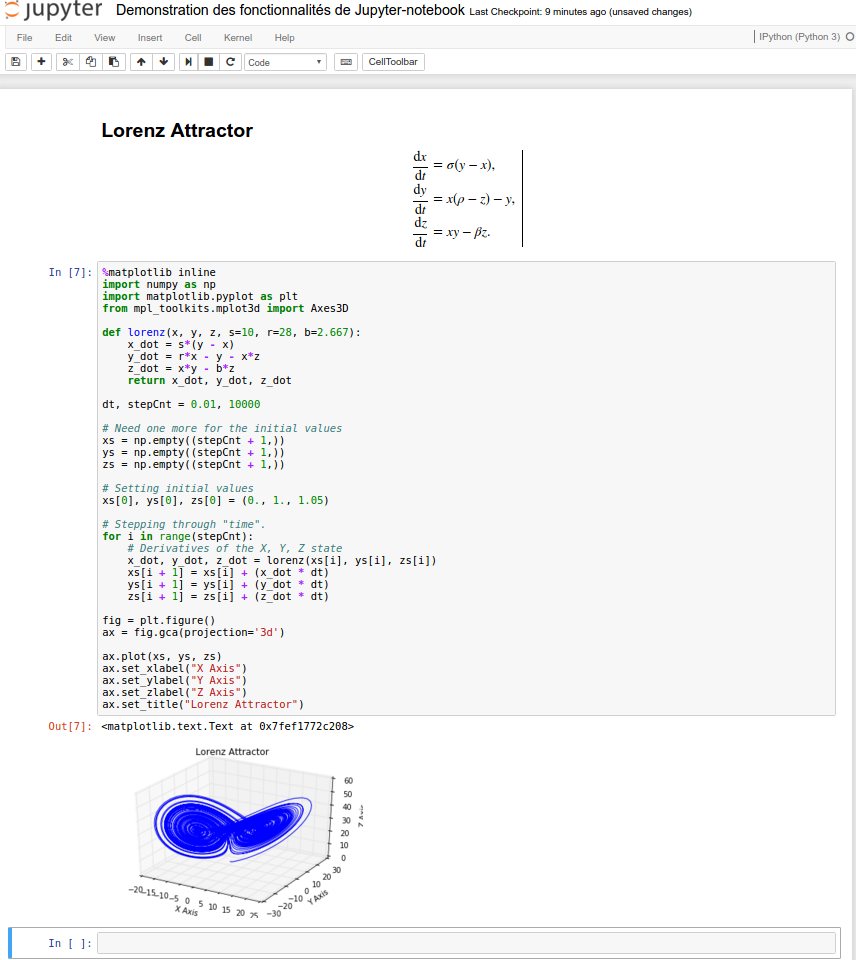
\includegraphics[width=.8\textwidth]{img/jupyter_demo2.png}
  \caption{Capture d'écran d'un notebook ouvert fonctionnant en local et consulté par interface web}
  \label{makesense:fig:demo}
\end{figure}

Un notebook, une fois lancé, peut être vu et utilisé via une interface graphique comme montré sur la Figure~\ref{makesense:fig:demo} qui met en jeu une interface web.
Cette figure met en jeu quatre cellules, la première représente un rendu de texte enrichi avec un titre mis en gras et des formules \LaTeX{} rendues et centrées.
Lorsqu'une cellule de texte est rendue, le texte et les formules mathématiques au format \LaTeX{} ou Markdown contenus  dans cette cellule sont rendus à l'utilisateur permettant d'avoir une mise en page avec des listes, des sections, des images et des formules mathématiques.

La seconde cellule est une cellule de code: elle contient du code et des ``built-in magic commands'' introduites par le signe \% au début de la cellule et servant à modifier dynamiquement le comportement du notebook.
Lorsqu'une cellule de code est rendue, le code est exécuté dans le noyau qui est un contexte commun pour toutes les autres cellules de code du notebook.
De plus, les cellules de code peuvent être ré-exécutées indépendamment les unes des autres permettant par exemple de séparer les calculs longs et coûteux des calculs plus courts d'exploration ou de visualisation de données.

Enfin, la troisième cellule montre le résultat de l'exécution du code contenu dans la seconde cellule sous forme graphique.
La quatrième cellule est une cellule de code disponible pour être éditée et exécutée de manière interactive.

L'utilisation des notebooks dans les logiciels scientifiques est ancienne et cette technologie est devenue suffisamment mature pour être utilisée aussi bien en recherche qu'en enseignement~\cite{gray1991exploring,young2003science,stevens2013automated,perez2013open}.

Parmi l'ensemble des notebooks libres disponibles, on peut citer Wakari~\cite{tsaftaris2014scientist}, Sage~\cite{stein2008sage}, Apache Zepplin~\cite{manivannan2015scala} ou encore IPython~\cite{PER-GRA:2007}.

Makesense intègre dans un notebook l'ensemble des traitements, paramètres, fonctions et la documentation du protocole expérimental d'une expérience sur les \ac{LLN}s.
Makesense peut fonctionner avec plusieurs formats de notebook différents tant qu'ils supportent certaines fonctionnalités.

Jupyter~\cite{poweredbyjupyter} est un projet proposant une suite d'outils libres pour l'informatique interactive et parallèle scientifique.
Ce projet est une évolution du projet IPython~\cite{PER-GRA:2007} qui a été étendu pour donner le projet Jupyter.
Le Jupyter Notebook est le format de notebook fournit par le projet Jupyter combinant code, texte, images, expressions mathématiques et des fonctions interactives au sein d'un même document qui est encodé dans un format texte documenté~\cite{notebookformat}.
Ces notebooks peuvent être lancés dans des interfaces graphiques ou web qui offrent un rendu graphique et un contexte d'exécution commun par l'utilisation d'un noyau.
Jupyter dispose d'une communauté d'utilisateurs et de développeurs large et dynamique ainsi que de nombreux ouvrages documentant son fonctionnement~\cite{mckinney2012python}.

Les paragraphes suivants détaillent les différents critères et justifient pourquoi Makesense utilise dans cette thèse la plateforme Jupyter et son format de notebook afin de documenter et effectuer des expériences.

\subsubsection{Propriétés recherchées pour un notebook}
\label{makesense:justification_notebook}

\paragraph{Format texte et ouvert}

Reproduire une expérience doit avoir aussi peu de barrières que possible, or acheter une licence ou un abonnement pour utiliser un logiciel propriétaire représente une barrière non négligeable.
Ainsi seuls les formats ouverts et pouvant être utilisés par des solutions libres sont pertinents pour un notebook visant à être utilisé par un public large.

Utiliser un format texte permet en outre de visualiser facilement les différences entre deux versions d'un même notebook par des outils de comparaisons de documents textes classiques ce qui permet de faciliter l'acceptation des contributions extérieures.
De plus, la gestion des révisions est nécessaire pour la mise en place d'une intégration continue efficace qui sera introduite dans la section~\ref{makesense:ci}.

Jupyter Notebook utilise un format texte ouvert et documenté sous la forme d'un \ac{JSON}~\cite{notebookformat} et répond donc à ce besoin fonctionnel.

\paragraph{Flexibilité dans le choix du langage de programmation}

Les préférences de langage de programmation peuvent varier en fonction d'une expérience et des préférences d'un utilisateur.
La notion de notebook est indépendante du langage qu'elle utilise, car c'est avant tout un format contenant du texte enrichi et de la mise en page de cellules.
Ainsi un notebook idéal doit être indépendant d'un langage de programmation donné pour laisser autant de flexibilité que possible à un utilisateur.

Le format de notebook de Jupyter Notebook est découplé de son noyau d'exécution, ainsi il existe plus d'une soixantaine de noyaux différents, écrits dans plusieurs langages de programmation~\cite{poweredbyjupyter}.
Les critères de choix d'un moteur sont relatifs à la disponibilité des bibliothèques logicielles, la stabilité du moteur et les propriétés du langage.

Afin de bénéficier de la plus grande stabilité et d'une large gamme de bibliothèques logicielles scientifiques, Makesense utilise \texttt{ipykernel} qui est le noyau historique de référence de Jupyter codé en Python.
De plus, l'utilisation de Python permet d'interfacer facilement Makesense avec la plateforme FIT-IoT-lab (\ref{automation:deploy_execute_move}) par l'utilisation de la bibliothèque officielle d'IoT-lab qui est codée en Python.

\paragraph{Support d'exports et de rendu}

Un notebook utilisé par Makesense doit pouvoir répondre à deux besoins relatifs au partage et l'export d'une expérience afin de pouvoir couvrir un large éventail d'utilisation et être flexible sur les préférences de leurs différents utilisateurs.

Le premier consiste à pouvoir être exportable vers des fichiers statiques (\ac{PDF}, page web, etc.) afin que les résultats d'une expérience puissent être partagés sans nécessiter une installation de dépendances et l'exécution des cellules.

Jupyter-notebook dispose d'un grand nombre d'exports et un rendu automatique des notebooks est supporté par plusieurs plateformes en ligne comme Github~\footnote{\href{https://github.com/sieben/makesense/blob/master/demo.ipynb}{https://github.com/sieben/makesense/blob/master/demo.ipynb}} et nbviewer~\footnote{\href{http://nbviewer.jupyter.org/}{http://nbviewer.jupyter.org}}.
Ainsi un notebook peut être rendu directement sur la plateforme Github pour avoir un rendu similaire à celui de la Figure~\ref{makesense:fig:demo} en ligne et sans installation.
Le rendu sur ces plateformes est fait sur une page web statique pouvant être imprimée ou partagée avec des relecteurs.

Le second besoin consiste à pouvoir extraire les cellules de code vers un programme exécutant l'ensemble de l'expérience.
Cette approche est pertinente pour disposer d'un programme pouvant ré-exécuter l'expérience et produire ses résultats et où le rendu du texte n'est pas souhaité.

Jupyter-notebook supporte ces deux types d'exports et permet ainsi à Makesense de répondre à ce besoin fonctionnel.

\subsection{Automatisation d'une expérience}
\label{makesense:auto}

Automatiser les tâches d'un processus est essentiel pour s'assurer qu'aucune étape n'a été oubliée et qu'elles sont toutes explicitées. 
Dans le cas de développement d'expériences collaboratives, automatiser permet d'éviter les configurations spécifiques d'une machine, et favorise la synchronisation du code et des résultats.

Makesense permet d'obtenir à partir du notebook d'une expérience son automatisation et de garantir sa reproductibilité.

Dans le cas de simulations, l'automatisation a pour but d'assurer que la construction, l’exécution et l'obtention des résultats sont valides et reproductibles.
Lorsque des paramètres aléatoires sont utilisés, pour par exemple injecter un bruit aléatoire sur un canal, un simulateur est complètement déterminé dès lors que la graine du générateur de nombres aléatoires est fixe et que les paramètres d'entrées sont constants.

Dans le cas des déploiements réels, les nœuds physiques utilisés pour réaliser une expérience peuvent changer en raison de pannes ou de problèmes d'exploitations, ce qui rend l'automatisation plus délicate, mais encore possible.
En outre, dans le cas d'expériences se déroulant sur une plateforme publique, une exécution peut être perturbée par les expériences gérées par d'autres utilisateurs par exemple pour les conditions radio.

Comme vu dans la section~\ref{makesense:justification_notebook}, il est possible de convertir un notebook en un programme par extraction des cellules de code qu'il contient. 
L'exécution de ce programme permet de refaire étape par étape une expérience automatiquement.

\subsubsection{Découpage d'une expérience en étapes}

\begin{figure}[ht]
  \begin{tikzpicture}[->,>=latex,shorten >=1pt,auto,node distance=3cm,
    thick,
    main node/.style={fill=blue!20,draw},
    pre node/.style={fill=red!20,draw},
    post node/.style={fill=green!20,draw}
    ]

    \node[pre node] (make) at (0, 3) {\begin{tabular}{c}Fabrication\end{tabular}};
    \node[pre node] (deploy) at (6, 3) {\begin{tabular}{c}Déploiement\end{tabular}};
    \node[pre node] (run) at (12, 3) {\begin{tabular}{c}Exécution\end{tabular}};

    \node[post node] (parse) at (12, -3) {\begin{tabular}{c}Mise en forme\end{tabular}};
    \node[post node] (analyze) at (6, -3) {\begin{tabular}{c}Analyse\end{tabular}};
    \node[post node] (plot) at (0, -3) {\begin{tabular}{c}Présentation\end{tabular}};
    
    % \node[main node] (analyze) at (12,0) {\begin{tabular}{c}Analyse\end{tabular}};

    \node[main node] (ipython) at (6,0) {\begin{tabular}{c}Fichier de configuration\\ \& \\Présentation\end{tabular}};

    \path
       (make) edge[ultra thick] node[above] {Firmwares \& Configs} (deploy) 
       (deploy) edge[ultra thick] node[above]  {Simulateur \& Testbeds} (run)
       (run) edge[ultra thick] node[right] {Traces brutes} (parse) 
       (parse) edge[ultra thick] node[below] {Traces mises en forme} (analyze)
       (analyze) edge[ultra thick] node[below] {Traitements de données} (plot)

  (ipython) edge[dashed] (make)
  (ipython) edge[dashed] (deploy)
  (ipython) edge[dashed] (run)
  (ipython) edge[dashed] (parse)
  (ipython) edge[dashed] (analyze)
  (ipython) edge[dashed] (plot)
  ;
  \end{tikzpicture}
  \caption{Découpage des étapes d'une expérience par Makesense}
  \label{makesense:fig:schema}
\end{figure}

Une expérience peut être découpée en différentes étapes qui se suivent dans un ordre logique.
Le schéma~\ref{makesense:fig:schema} illustre comment les différentes étapes d'une expérience typique à propos des \ac{LLN}s se suivent.

La \emph{fabrication} produit tous les binaires et fichiers de configurations initiaux qui sont nécessaires à une expérience.
La phase de \emph{déploiement} déplace ces fichiers sur les bonnes machines.
La phase d'\emph{exécution} lance et maintient les processus nécessaires à une expérience et produit les traces brutes qui correspondent aux grandeurs mesurées.
La phase de \emph{mise en forme} ``nettoie'' des traces brutes afin de les rendre plus simples à analyser et exploiter.
La phase d'\emph{analyse} traite ces données mises en forme afin de produire des analyses qualitatives et quantitatives sur les phénomènes observés.
Enfin, la phase de \emph{présentation} fournit les représentations graphiques qui seront le plus souvent mises dans des articles ou partagées avec d'autres collaborateurs.

Chacune des cellules de code utilisée peut être précédée ou suivie de plusieurs cellules de textes enrichis pour décrire ce qu'elle contient ou apporter des précisions sur son fonctionnement.
Les résultats intermédiaires des cellules de code peuvent être conservés dans le contexte commun à toutes les cellules du notebook, ce qui permet de réutiliser des résultats et au besoin d'ajouter une nouvelle cellule pour explorer une nouvelle idée.

\subsubsection{Expérience séquentielle et script d'exécution}
\label{makesense:sequentiel}

Comme vu dans la section~\ref{makesense:related_automatisation}, il est nécessaire d'utiliser un outil de gestion de dépendance de tâches pour s'assurer que toutes les dépendances d'une tâche sont exécutées.
Or comme l'illustre le schéma~\ref{cache:fig:schema}, une expérience typique est bâtie autour d'un succession séquentielle d'étapes.
Ainsi l'organisation du code d'un notebook en succession d'étapes est acceptable pour ce type d'expérience rendant les outils génériques de gestion de dépendances de tâches tel que \texttt{make} non nécessaire par rapport aux besoins.

Il est donc possible de mettre chacune des étapes d'une expérience dans une cellule spécifique, ce qui permet de rendre une expérience modulaire, car on peut obtenir le résultat d'une étape donnée en exécutant seulement une fois ses dépendances et en conservant les résultats intermédiaires.
Ce découpage permet de ne pas imposer de formalismes lourds sur une expérience et permet d'avoir une grande flexibilité sur son organisation.

Ce flot séquentiel est également adapté pour fournir un programme validant une par une toutes les étapes pour aboutir à la production des résultats.
Ce programme séquentiel est obtenu par l'extraction des cellules de code du notebook qui fournissent un programme pouvant reproduire l'exécution complète de l'expérience.
Ainsi il est possible de tirer parti de ce programme pour tester de manière systématique que l'expérience fonctionne d'une révision à l'autre.

\subsection{Garantie de reproductibilité d'une expérience}

Une expérience doit évoluer au cours du temps afin de corriger ses erreurs et obtenir de nouveaux résultats.
Cependant cette évolution ne doit pas se faire au détriment de la stabilité des résultats précédemment obtenus, car un processus expérimental se construit sur des acquis pour ensuite les étendre.

Un processus de développement logiciel efficace doit garantir une conservation des différentes révisions afin de revenir en arrière si une erreur est introduite ou bien de gérer les révisions concurrentes de plusieurs contributeurs.
Ainsi des logiciels spécifiques ont été introduits pour tenir compte de ces révisions et les gérer efficacement.
Les gestionnaires de versions sont aujourd'hui une fondation du développement logiciel et sont largement utilisés~\cite{o2009making}.

Makesense utilise un gestionnaire de révisions afin de garder en mémoire les différentes révisions d'un notebook.
L'observation des différences entre les différentes révisions est importante pour comprendre comment chaque révision modifie un notebook donné.
\texttt{git} est le gestionnaire de révision de référence de Makesense car il permet de disposer depuis la plateformes Github d'un rendu automatique du notebook pour toutes ces révisions successives~\cite{loeliger2012version,dabbish2012social}.
Cependant, Makesense est complètement agnostique sur le gestionnaire de version utilisé et ne l'utilise que pour mettre en place des mécanismes d'intégration continue.

\subsubsection{Intégration continue}
\label{makesense:ci}

L'obsolescence d'un programme peut arriver quand aucun test n'est présent pour s'assurer qu'il fonctionne ou non au cours de ses révisions successives.
Pour éviter cette obsolescence, il est nécessaire d'utiliser un processus systématique qui va vérifier à chaque révision que les résultats précédemment obtenus sont toujours valides.
Comme vu dans la section~\ref{makesense:sequentiel}, un notebook peut être transformé en script qui va exécuter séquentiellement une expérience pour en fournir les résultats.

L'\emph{intégration continue} est un ensemble de pratiques utilisées en production de logiciel qui consiste à vérifier que chaque modification apportée à un programme ne modifie pas son fonctionnement et qu'aucune régression fonctionnelle n'est introduite~\cite{duvall2007continuous}.
Son principal but est de détecter les problèmes et les erreurs afin de les corriger au plus tôt et de raccourcir les cycles de développement.
Massivement pratiquée par les acteurs principaux du développement logiciel elle a engendré de nouveaux courants et méthodologies logicielles comme le \ac{TDD}~\cite{beck2003test} qui ont prouvé leur efficacité pour réduire le nombre d'erreurs au cours du développement d'un logiciel~\cite{maximilien2003assessing}. 

L'intégration continue est déclenchée quand une proposition de changement \footnote{``pull request'' dans le cas où on utilise \texttt{git}.} est poussée vers le dépôt gérant les versions du notebook.
Une copie de la version révisée est envoyée sur le serveur d'intégration continue qui va créer l'environnement pour le notebook, extraire les cellules de code puis exécuter le programme engendré.
Une fois l'exécution terminée et sans erreur, on a la garantie que le changement n'a pas engendré une erreur sur un résultat existant~\footnote{On parle de test de non-régression.}.
Une fois que le résultat est conforme aux tests demandés, il peut être intégré à la branche principale de développement et le processus se répète pour tout nouveau changement proposé.

Cette méthodologie de développement logicielle combinée a un script extrait d'un notebook permet de garantir que l'expérience contenue reste reproductible.

L'intégration continue dans le cas d'expérience sur un \ac{LLN} garantit que toutes les dépendances requises pour créer une expérience, l'exécuter et exploiter les résultats sont documentées, installées avec une intégration testée et fonctionnelle.

Makesense versionne l'évolution du notebook contenant l'expérience de cette section en utilisant \texttt{git} et en l'hébergeant sur Github.
Lorsqu'une nouvelle révision est proposée (pour ajouter une étape, changer une variable), une proposition de révision est envoyée pour être relue par les propriétaires du dépôt hébergeant le notebook.
Lorsque la proposition de révision est initiée, une copie de la version modifiée est envoyée vers le serveur d'intégration continue qui déterminera si cette révision est acceptable.
Cette vérification est obtenue en procédant à l'extraction des cellules de code du notebook et l'exécution du script obtenu.
Une fois cette vérification faite, la révision peut être intégrée au dépôt du notebook et ce cycle se répète à chaque révision proposée.

\subsection{Approvisionnement d'une expérience}

L'approvisionnement d'une expérience consiste à préparer tous les fichiers et systèmes nécessaires au déroulement d'une expérience.
Les expériences sur \ac{LLN}s mettent en jeu des nœuds ayant des configurations spécifiques par exemple sur la fréquence d'envoi d'un message.
Configurer chaque nœud de manière ad hoc n'est pas envisageable à mesure que le nombre de nœuds et les paramètres mis en jeu grandissent.
Afin de réaliser des expériences à grande échelle, le langage utilisé pour décrire l'expérience doit être suffisamment souple et expressif pour initialiser facilement chaque nœud à partir d'un modèle de base.

La mise en œuvre de cette phase de configuration dans Makesense consiste à créer à partir de gabarits de base (appelé ``template'' en anglais), les fichiers qui seront utilisés et compilés au cours de l'expérience.
Chaque fichier nécessaire à l'expérience va être construit à partir d'un gabarit de base qui va être rempli par un moteur de gabarit (aussi appelé ``templating engine'' en anglais) avec les variables qui lui sont propres.
Ce type de pratique par gabarit a déjà été utilisé et validé à large échelle dans le contexte de configuration de serveurs et de configuration de serveurs~\cite{hochstein2014ansible} ainsi son utilisation dans le contexte de la configuration des nœuds capteurs se rapproche de cette utilisation.

Dans le cas typique des expériences portant sur un \ac{LLN}, cette étape de préparation compile les systèmes d'exploitation pour les nœuds contraints et produit tous les fichiers de configuration nécessaires à la simulation.
Dans le cas du binaire exécuté par les nœuds, il est obtenu pour différentes architectures~\footnote{L'émulation dans COOJA s'effectue sur l'architecture MSP430 et les nœuds FIT-IoT-lab utilisent l'architecture ARM dans le cas des Cortex M3.}.

Une simulation dans Cooja requiert la création d'un fichier principal qui va être utilisé pour placer les nœuds, les démarrer avec le bon binaire, interagir avec eux, configurer leur portée de transmission ou la graine des générateurs de nombres aléatoires utilisée pendant la simulation.
Ainsi, Makesense fournit un gabarit de fichier de configuration qui est peuplé dynamiquement et enregistré pour être utilisé ensuite.
Le rendu de la topologie est fait automatiquement et les binaires sont compilés correctement avec leurs variables propres et sont affectés aux nœuds correspondants dans le fichier de configuration de la simulation.

\subsection{Déploiement - Exécution et récupération des traces}
\label{automation:deploy_execute_move}

L'objectif des phases de déploiement, d'exécution et de déplacement des traces est de produire une exécution de l'expérience visée et de déplacer toutes les traces pertinentes de cette expérience vers une destination spécifique pour y être analysées.
Cette phase est délicate car elle met en jeu de nombreux processus.
Elle est documentée et automatisée par Makesense afin de fournir autant que faire se peut une reproductibilité de l'expérience qu'elle se passe dans un simulateur ou sur plateforme.

\subsubsection{Déploiement}

La phase de déploiement déplace les fichiers produits lors de l'approvisionnement vers la machine où ils seront utilisés.

Makesense déploie une expérience vers un serveur ou une plateforme en utilisant les \ac{API} ou un accès à distance automatisable.
Ainsi toute plateforme ou machine utilisant un accès à distance automatisable est utilisable par Makesense.

Dans le cas de l'exécution d'une simulation sur la même machine, ce déploiement correspond à une simple copie des fichiers pertinents.
Cependant, dans le cas de simulations devant être exécutées sur des grilles de calcul, il est nécessaire de mémoriser sur quels serveurs l'expérience a été déployée afin d'en récupérer les résultats.

L'utilisation d'un testbed permet de confirmer les résultats d'un simulateur par une exécution de l'expérience sur des nœuds physiques.
Dans le cas de testbeds mutualisés, il faut gérer des réservations de nœuds qui sont potentiellement accessibles par tous les utilisateurs de la plateforme et qui peuvent également tomber en panne.
Ainsi il est nécessaire de maintenir dynamiquement une table de correspondance entre les  nœuds réservés et le code qui y est exécuté.
Automatiser ce processus de déploiement permet de choisir dynamiquement les nœuds mis en jeu lors d'une expérience (par exemple les moins chargés, les mieux placés, etc.).

Plusieurs testbeds publics tels que Indriya~\cite{doddavenkatappa2011indriya} ou bien IoT-lab~\cite{fleury2015fit} sont disponibles afin d'exécuter une expérience sur des nœuds physiques.
Makesense supporte IoT-lab par l'utilisation de la bibliothèque officielle pour réserver et démarrer des expériences.
La plateforme IoT-lab a été choisie en raison de la variété des nœuds physiques proposés, du support des systèmes d'exploitation de référence sur ses nœuds et de son processus de réservation et d'accès à distance facilement automatisable.
IoT-lab met à disposition de ses utilisateurs, sur plusieurs sites physiques ayant la même interface, des nœuds physiques supportant \ieee{} représentatifs de nœuds capteurs.
Pour fonctionner, IoT-lab utilise, entre autre, des serveurs (nommés ``front-end'') sur lesquels des utilisateurs peuvent se connecter par \ac{SSH} et lancer des commandes visant à interagir avec les nœuds physiques.
Makesense utilise la bibliothèque officielle d'IoT-lab afin de faire les réservations et d'envoyer les binaires utilisés par les nœuds physiques.
Dans le cas où d'autres programmes doivent être déployés sur les serveurs d'IoT-lab, Makesense y accède par \ac{SSH} afin d'y envoyer les fichiers requis.

\subsubsection{Exécution}

Lors de l'exécution d'une expérience, il est courant d'avoir plusieurs processus lancés en parallèle pour effectuer différentes fonctions.
Parmi ces processus, certains vont par exemple, générer les traces brutes qui vont être utilisées par la suite pour analyser le déroulement d'une expérience.

Ces processus sont parfois nombreux, s'exécutent avec différents privilèges, sur différentes machines et dans un certain ordre.
En outre, il faut s'assurer qu'une fois lancés, ces processus continuent de fonctionner correctement durant toute l'expérience.
Gérer manuellement ces processus comporte plusieurs risques, d'une part, il est possible d'en oublier un ou bien de les lancer dans le désordre causant l'échec de l'expérience si ces processus sont critiques.
De plus, dans le cas où les expériences durent longtemps, il est nécessaire de maintenir une surveillance continue de l'expérience et de chacun de ces processus.

Makesense permet de documenter le lancement de ces processus en les mettant dans des objets qui sont gérés de manière automatisée.
Ainsi les processus sont systématiquement lancés et dans le même ordre permettant d'éviter les écueils d'un lancement manuel.
D'autre part, il est possible d'avoir au cours de l'exécution le statut d'un processus et le relancer le cas échéant.

\subsubsection{Récupération des traces}

Une expérience, qu'elle se produise dans un simulateur ou sur nœuds physiques, génère de nombreuses données brutes comme des fichiers \ac{PCAP}~\cite{mccanne1989libpcap} qui décrivent le trafic réseau ou encore des journaux d’événements (appelés ``logs'' en anglais).

Afin de simplifier les traitements, il est pratique de rassembler toutes ces traces sur une seule machine qui va être utilisée pour traiter ces données.
Ainsi il est nécessaire d’agréger les différents fichiers de données en provenance de sources multiples vers une seule destination.
Automatiser ces traitements permet de garantir qu'aucun de ces fichiers n'est oublié, de documenter ceux qui seront traités et ceux non pertinents qui seront évités.

Makesense peut déplacer toutes les traces brutes depuis une machine donnée (par exemple une grille de calcul ou un front end IoT-lab) vers une autre (par exemple une station de travail locale ou un ordinateur portable).

Dans le cas d'une expérience sur IoT-lab, l'identifiant d'expérience qui est donné lors de la réservation d'une expérience permet d'obtenir l'adresse du dossier contenant les résultats sur le serveur front end.
Ainsi Makesense récupère les traces dynamiquement en fonction de cet identifiant et sur l'ensemble des fichiers pertinents ce qui est plus efficace qu'une récupération manuelle de chaque fichier individuel.

\subsection{Exploitation des résultats}

L'exploitation de résultats est la phase permettant d'étudier de manière quantitative et qualitative une expérience en utilisant ses traces.
Les étapes que cette phase comporte étant dissociées des contraintes des \ac{LLN}s, tous les traitements peuvent utiliser des outils généraux et communs à de nombreux champs de recherche scientifique.
Cette phase est complètement automatisable et déterministe, car elle applique des traitements fixes à des traces fournies en amont.
L'objectif de cette phase consiste d'une part à décoder toutes les traces brutes pour en extraire les informations les plus pertinentes et d'autre part à fournir des données pour une interprétation quantitative et qualitative de l'expérience.

\begin{figure}[ht]
\centering
\begin{tikzpicture}[->,>=latex,shorten >=1pt, thick,main node/.style={fill=blue!20,draw}]

  \node[main node] (parse) {\begin{tabular}{c}Mise en forme\end{tabular}};

  \node[main node, below left=of parse] (pcap) {\begin{tabular}{c}PCAP\end{tabular}};
  \node[main node, above left=of parse] (logs) {\begin{tabular}{c}Logs\end{tabular}};

  \node[main node, right=of parse] (good_data) {\begin{tabular}{c}Données mises en forme\end{tabular}};
  \node[main node, above=of good_data] (analysis) {\begin{tabular}{c}Analyse des données\end{tabular}};

  \node[main node, below=of good_data] (csv) {\begin{tabular}{c}Export vers CSV\end{tabular}};


  \path
       (pcap) edge[->] (parse.south west) 
       (logs) edge[->] (parse.north west) 
       (parse) edge[->] (good_data) 
       (good_data)  edge[->] (analysis)
       (good_data) edge[->] (csv) 
  ;

\end{tikzpicture}
\caption{Transformation des traces brutes vers des formats de données standards}
\label{makesense:fig:data_clean}
\end{figure}

La Figure~\ref{makesense:fig:data_clean} illustre l'approche choisie par Makesense.
Le processus de transformation vise à aboutir à des données mises en forme qui seront exploitées directement lors de la phase d'analyse et qui peuvent être exportées au besoin vers un format standard pour être partagées.

\subsubsection{Mise en forme de traces brutes}

Les traces brutes sont de nature hétérogène, une première étape de la phase de traitement consiste à transformer ces résultats bruts vers des fichiers plus exploitables et homogènes.
L'objectif de cette approche est de distinguer la phase de décodage d'une trace de son interprétation.

Dans le cas d'une expérience portant sur les \ac{LLN}s, il s'agit par exemple de transformer les fichiers \ac{PCAP} et les multiples journaux textes représentant les événements qui se sont produits par des transformations pour obtenir des traces plus exploitables.

Une conversion ad hoc aurait du mal à fonctionner pour un grand nombre de fichiers et de traitements différents.
En outre, documenter les traitements effectués permet d'avoir une documentation sur les formats de documents obtenus afin d'éviter les traitements ad hoc.
Enfin, transformer les données vers un format standard comme \ac{CSV} permet de les importer dans de nombreux outils plus facilement notamment dans le cas de données tabulaires.
Ainsi les mêmes traces peuvent être réutilisées pour des expériences voulant explorer différentes conclusions autour de données communes.

Makesense implémente ces transformations en utilisant des bibliothèques logicielles dédiées aux traitements de données tabulaires.
L'objectif est d'appliquer à chaque élément d'une trace toutes les transformations nécessaires (renommage, normalisation, etc.) afin d'obtenir des tableaux et d'autres structures de données facilement exportables et manipulables.

\subsubsection{Analyse des résultats}

La phase d'analyse de résultats traite les données mises en forme afin de permettre leur interprétation et de fournir des résultats qualitatifs ou quantitatifs sur une expérience.
Elle doit être facilitée par des itérations aussi courtes que possible pour tester de nouvelles hypothèses afin de diminuer le temps nécessaire pour confirmer ou infirmer une hypothèse sur une expérience.

Makesense met à profit des bibliothèques logicielles scientifiques afin d'effectuer ces traitements~\cite{mckinney2012python}.
Les données mises en forme sont chargées dans des structures de données tabulaires où il est facile de les filtrer sur certains critères et de les agréger par différentes fonctions (une somme, un comptage, etc.).
Le rendu de ces données peut être fait sous forme graphique avec des graphes qui illustrent les phénomènes observés.

Dans le cas d'expériences sur les \ac{LLN}s, il est par exemple nécessaire d'exploiter les données disponibles dans les traces de trafic réseau en utilisant un dissecteur de paquets comme Wireshark~\cite{tshark}.
Ces traces présentées dans le notebook sous la forme de tableau représentent pour chaque paquet les attributs trouvés par le dissecteur (source, destination, protocole, taille, etc.).
Ainsi pour analyser la répartition de protocoles réseau, il suffit d'effectuer une requête similaire sémantiquement à une requête faite sur une base de données relationnelle classique~\cite{mckinney2012python}.
Ce formalisme permet une grande expressivité sur les données recueillies et permet de s'abstraire des représentations concrètes des données dans les fichiers pour se concentrer sur ce qu'elles représentent.
Ces données une fois trouvées peuvent être représentées par des visualisations et des graphes par des outils graphiques~\cite{Hunter:2007}.

Un autre exemple consiste à avoir une représentation graphique de la topologie du réseau formée par les nœuds directement dans le notebook.
Cela permet d'identifier rapidement les dysmétries et les nœuds importants pour la connexité du graphe.
De plus, une fois cette représentation du \ac{DODAG} \ac{RPL} disponible, il est possible de calculer les plus courts chemins entre un nœud et la racine du \ac{DODAG} afin d'obtenir la profondeur d'un nœud.

Ces fonctionnalités de groupement d'informations permettent d'exprimer de manière concise des traitements sur les données pour en extraire les informations utiles.

\section{Conclusion} 
\label{makesense:conclusion}

Ce chapitre montre qu'afin de permettre le partage et la reproductibilité d'une expérience, sa documentation et son automatisation jouent un rôle clé.
Ce processus est assez systématique et dépasse largement le contexte des \ac{LLN}s, ainsi des méthodologies et des outils communs peuvent émerger pour proposer des solutions à des problèmes communs.

Makesense est une réponse possible et se veut générique en utilisant des bibliothèques généralistes et répandues dans de multiples domaines de développement logiciel scientifique ou général.
Makesense propose de documenter et d'automatiser une expérience pour \ac{LLN} transcrite dans un notebook pour s'assurer de sa reproductibilité.
La reproductibilité d'une expérience est une nécessité des projets de recherche.
La réduction de la complexité de la mise en place d'une expérience permet d’accélérer une étude et d'augmenter son impact en facilitant sa vérification et son partage.
À cette fin, Makesense est disponible sous licence Apache sur Github~\footnote{\href{https://github.com/sieben/makesense}{https://github.com/sieben/makesense}} et une démonstration du déroulement d'une expérience est également disponible~\footnote{\href{https://travis-ci.org/sieben/makesense}{https://travis-ci.org/sieben/makesense}}.
Étant diffusé sous licence libre, il est difficile d'estimer son utilisation globale, cependant la version initiale disponible sur PyPI a été téléchargée plus de 1000 fois.

Makesense a été utilisé afin de réaliser les expériences décrites dans les chapitres précédents et pourrait être mis à profit afin d'avoir une solution permettant d'avoir une intégration complète d'une expérience dans le but de la diffuser.

Makesense ne gère pas pour le moment les erreurs à la volée qui peuvent subvenir lors d'une expérience.
Or dans le cas de tests sur nœuds réels, ces erreurs peuvent être nombreuses par exemple dans le cas d'erreurs de flashage ou de panne d'un nœud.
Il est alors nécessaire de redémarrer le nœud brutalement et cela ne garantit pas que le problème n'arrivera pas de nouveau.

Avoir une gestion plus fine et réactive des processus permettrait de prendre des décisions plus raisonnées dans le but d'avoir un environnement plus contrôlable.
Cependant cette tâche est délicate, car les pannes et problèmes qui peuvent subvenir sont très hétérogènes et il est difficile de prendre des décisions automatiques dans ce genre de cas notamment dans le cas de testbeds mutualisées ou le contrôle de l'environnement et de ses interférences n'est pas facilement réalisable.

Une autre fonctionnalité pourrait être la gestion de points d'étapes (``checkpoint'' en anglais) dans une expérience qui permettrait de sauvegarder l'intégralité du contexte d'une expérience à un instant donné.
Cette fonctionnalité serait particulièrement utile pour effectuer des analyses post mortem d'un système tombé en panne.

Les méthodologies modernes de développement logiciel peuvent influencer les méthodologies expérimentales scientifiques notamment en informatique où de nombreux outils sont communs.
La création de communautés autour des différents outils logiciels utilisés par la communauté scientifique facilite les échanges et la diffusion de nouvelles méthodes plus efficaces pour résoudre les problèmes communs.
Makesense illustre comment intégrer efficacement ces technologies afin d'aider les expériences sur les \ac{LLN}s à être plus reproductibles.
Ce framework est mis à profit dans les expériences des chapitres~\ref{cache} et~\ref{supervision}.

\section*{Publications et invitations relatives à Makesense}

\begin{itemize}
  \item Rémy Leone, Jeremie Leguay, Paolo Medagliani, Claude Chaudet, et~al.
\newblock Makesense: Managing reproducible wsns experiments.
\newblock {\em Fifth Workshop on Real-World Wireless Sensor Networks}, 2013.

  \item Rémy Léone, Jérémie Leguay, Paolo Medagliani, and Claude
  Chaudet.
\newblock Demo abstract: Makesense—managing reproducible wsns experiments.
\newblock In {\em Real-World Wireless Sensor Networks}, pages 65--71. Springer,
  2014.

  \item Rémy Léone, Jérémie Leguay, Paolo Medagliani, and Claude
  Chaudet.
\newblock Demo Abstract: Automating WSN experiments and simulations.
\newblock In {\em EWSN}, 2015.

  \item Invitation au colloque R4: Retour d'expéRiences sur la Recherche Reproductible.
  \newblock Le Studium - Centre International Universitaire pour la Recherche - Orléans
  \newblock 3 et 4 décembre 2015 

\end{itemize}

%!TEX root = ../main.tex
% !TeX spellcheck = fr_FR

\chapter{Conclusion et perspectives}
\label{conclusion}

\section{Passerelle avancée pour les \ac{LLN}s}

L'augmentation du nombre d'appareils connectés est continue et apporte de nouveaux défis pour l'intégration de ces sources de données dans les réseaux classiques existants.
En raison de leur hétérogénéité, les nœuds des \ac{LLN}s peuvent utiliser des technologies de communications différentes pour apporter une solution de connectivité efficace en fonction de leur environnement.
La cohabitation de ces technologies semble inévitable car elles sont caractérisées par des compromis différents (bande passante, portée, consommation énergétique).
Cette hétérogénéité des standards et des protocoles implique l'utilisation de solutions d'interconnexion qui sont le plus souvent bâties autour du protocole IPv6 et d'une passerelle se trouvant à la bordure de ces réseaux.
Cette passerelle dispose de plusieurs radios lui permettant de communiquer physiquement mais aussi d'héberger des services supplémentaires par des fonctionnalités logicielles ou virtualisées en raison de ses ressources matérielles plus importantes.
Ces services peuvent mitiger les problèmes d'interopérabilité car ils peuvent ajouter de manière logicielle du support de protocoles et de services tiers afin d'offrir de l'interopérabilité et de la découverte de services.
Ainsi la passerelle peut devenir une plateforme sur laquelle de multiples services spécifiques aux \ac{LLN}s peuvent être instanciés afin de notamment améliorer leurs performances ou leur fiabilité.

Cette thèse a présenté comment la passerelle qui est utilisée pour connecter un \ac{LLN} à un réseau classique peut héberger des services pouvant optimiser de manière transparente l'utilisation des ressources d'un \ac{LLN}.
Le chapitre~\ref{gw} a permis de montrer comment la passerelle du fait de sa position peut avoir accès à une grande quantité d'informations concernant le \ac{LLN}.
À partir de ces informations, plusieurs mécanismes permettant l'optimisation des ressources des \ac{LLN}s ont étés proposés:

\begin{figure}[ht]
  \centering
  \pgfdeclarelayer{supervision}
  \pgfdeclarelayer{lln}
  \pgfdeclarelayer{proxy}
  \pgfsetlayers{supervision,lln,proxy,main}
  \begin{tikzpicture}

  % définition des styles
  \tikzstyle{visible}=[draw, fill=blue!50]
  \tikzstyle{hidden}=[ draw, fill=gray!20]
  \tikzstyle{router}=[circle, draw, fill=orange!50,text=black]
  \tikzstyle{child}=[circle, draw, fill=yellow!50,text=black]
  \tikzstyle{root}=[circle, draw, fill=red!50,text=black]



  % Réseau contraint
  \node[root] (1) at (-4, 0) {};
  \node[router] (2) at (-5, 1) {};
  \node[child] (3) at (-5, -1) {};
  \node[child] (4) at (-6, 2) {};
  \node[child] (5) at (-6, 0) {};

  % les nœuds
  \node[draw, right=2cm of 1] (lbr) {\ac{LBR}};
  \node[draw, right=of lbr] (rpca) {\ac{RPCA}};
  \node[draw, above=of lbr] (supervision) {Supervision passive};

  % \node[cloud, cloud puffs = 10, minimum width = 4cm, draw, fill = gray!10] (cloud) at (5,0) {Réseau local};
  \node[draw, right=of rpca] (cloud) {Réseau local};

  \node [fit=(1) (2) (3) (4) (5), rounded corners, draw=black!50] (lln) {};
  \node [fit=(lbr) (rpca), rounded corners, dashed] (gw) {};
  \node [below=.3 cm of lln] {LLN};
  \node [below=.3 cm of gw] {Passerelle};

  \node [fit=(lbr) (rpca) (supervision), rounded corners, draw=black!50] (gw) {};

\path

  % Réseau contraint
  (lbr.west) edge[<->, very thick, ForestGreen] (1)
  (1) edge[<->, very thick, bend left=20, ForestGreen] (2)
  (1) edge[<->, very thick, bend left=20, ForestGreen] (3)
  (2) edge[<->, very thick, bend left=20, ForestGreen] (4)
  (2) edge[<->, very thick, bend left=20, ForestGreen] (5)

  (1) edge[<->, very thick, dashed, bend right=20, Sepia] (2)
  (1) edge[<->, very thick, dashed, bend right=20, Sepia] (3)
  (2) edge[<->, very thick, dashed, bend right=20, Sepia] (4)
  (2) edge[<->, very thick, dashed, bend right=20, Sepia] (5)


  % Réseau conventionnel
  (rpca.west) edge[<->, very thick, ForestGreen] (lbr.east)
  (rpca.east) edge[<->, very thick, Cyan] (cloud)
  (lbr.north) edge [->, very thick, ForestGreen] (supervision.south)
  % (lbr) edge [->, dashed, out=270, in=270] (rpca.south)
  ;

\end{tikzpicture}

  % \begin{tikzpicture}[decoration={brace}]

  %   % Reverse proxy
  %   \begin{pgfonlayer}{proxy}
  %     \node[] (rpca) {
  %       \begin{tikzpicture}
  %         \node[draw] (proxy) {Reverse proxy/Cache};
  %         \node[draw, right=of proxy] (adapt) {Mécanisme d'adaptation};

  %         \path
  %         (proxy) edge[->, bend left=30, very thick] node[above] (topo) {Topologie, Trafic entrant} (adapt)
  %         (adapt) edge[->, bend left=30, very thick] node[below] (cache) {Temps de cache optimaux} (proxy)
  %         ;


  %         \node [fill=red!30, fit=(proxy) (adapt) (topo) (cache), rounded corners, draw=black!50]  {};

  %         \node[draw] (proxy2) {Reverse Proxy Cache};
  %         \node[draw, right=of proxy] (adapt) {Mécanisme d'adaptation};

  %         \path
  %         (proxy) edge[->, bend left=30, very thick] node[above] (topo) {Topologie, Trafic entrant} (adapt)
  %         (adapt) edge[->, bend left=30, very thick] node[below] (cache) {Temps de cache optimaux} (proxy)
  %         ;          
  %       \end{tikzpicture}
  %     };
  %   \end{pgfonlayer}

  %   % Cloud
  %   \node[cloud, cloud puffs = 10, minimum width = 7cm, draw, above=3cm of proxy, fill = gray!10] (cloud) {Réseau local};
  %   % \node[draw, above=3cm of proxy, fill = gray!10] (cloud) {Réseau};



  %   % LLN Border Router + LLN
  %   \begin{pgfonlayer}{lln}

  %     \node[draw, fill=green!30, below=5cm of proxy,](llnBorder) {
  %       \begin{tikzpicture}
  %         \tikzstyle{router}=[circle, draw, fill=orange!50,text=black]
  %         \tikzstyle{child}=[circle, draw,fill=yellow!50,text=black]
  %         \node[draw] (lbr) {Routeur de bordure}
  %         child {node[router]{}
  %           child {node[child]{}}
  %           child {node[child]{}}
  %         }
  %         child {node[router]{}
  %           child {node[child]{}}
  %           child {node[child]{}}
  %         };
  %       \end{tikzpicture}
  %     };  

  %   \end{pgfonlayer}

  %   % Supervision passive
  %   \begin{pgfonlayer}{supervision}

  %     \node [fill=yellow!30, above right=.5cm of llnBorder.north, rounded corners, draw=black!50] (supervision) {
  %       \begin{tikzpicture}

  %         \node[above right=.1cm of llnBorder.north]
  %         (eye) {
\includegraphics[scale=.5,angle=30]{img/eye.pdf}};


  %         \node[draw, right=.1cm of eye.east] (trafic) {Trafic};
  %         \node[draw, right=of trafic] (topo) {Topologie connue?};
  %         \node[draw, below right=.5cm of topo, text width=2.2cm,align=center] (star) {Estimation ``étoilée''};
  %         \node[draw, above right=.5cm of topo, text width=2.2cm,align=center] (mesh) {Estimation ``maillée''};
          
  %         % \node[draw, below=of trafic] (active) {Supervision active};

  %         \path
  %         (trafic) edge[very thick, ->] (topo)
  %         (topo) edge[very thick, ->,] node[above, left] {Non} (star.west)
  %         (topo) edge[very thick, ->,] node[below, left] {Oui} (mesh.west)
  %         % (trafic.east) edge[very thick, ->, bend right=30, dashed] node[below] {Topologie} (estimateur.west)
  %         % (active.east) edge[->, bend right=30] node[right=.3cm, text width=3cm] {Corrige le biais d'estimation} (estimateur.south west)
  %         ;

  %         % \draw[<->, >=latex, very thick] (active.west) to[out=180,in=90] (llnBorder.north);

  %       \end{tikzpicture}
  %     };
  %   \end{pgfonlayer}

  %   % Summary
  %   \node [fit=(supervision) (rpca) (lbr) (topo) (cache) (proxy), rounded corners, draw=black!50, very thick,dashed] (completeGateway) {};

  %   % Trafic
  %   \path
  %   (rpca) edge[>=latex, <->, line width=5pt] node[left] {HTTP} (cloud)
  %   (rpca) edge[>=latex, <->, line width=2pt] node[left] {CoAP} (llnBorder);

  %   % Brackets

  %   \tikzstyle{bracket}=[decorate,decoration={brace,amplitude=10pt,mirror,raise=4pt},line width=3pt]

  %   % \draw [bracket] 
  %   % ([yshift=-1cm]cloud.south east) -- ([yshift=1cm]cloud.north east) node [black,midway,xshift=2.3cm] {Réseau conventionnel};

  %   \draw [bracket]
  %   ([yshift=-5pt]completeGateway.south east) -- ([yshift=5pt]completeGateway.north east) node [black,midway,xshift=1.5cm] {Passerelle};


  %   \draw [bracket] 
  %   ([yshift=-5pt]rpca.south east) -- ([yshift=5pt]rpca.north east) node [black,midway,xshift=3cm] {Reverse Proxy Cache Adaptatif};

  %   \draw [bracket] 
  %   ([yshift=-5pt]llnBorder.south east) -- ([yshift=5pt]llnBorder.north east) node [black,midway,xshift=1cm] (llnBracket) {LLN};

  % \end{tikzpicture}

  \caption{Schéma de la passerelle proposée}
  \label{conclusion:schema}
\end{figure}

La Figure~\ref{conclusion:schema} illustre les contributions proposées dans cette thèse pouvant être déployées à la passerelle.
Ces contributions sont détaillées ci-après.

\subsection{Supervision}

Le chapitre~\ref{supervision} a proposé une méthode de mesure implicite de l'utilisation de la radio en s'appuyant d'une part sur le trafic observé par le routeur de bordure et d'autre part sur la topologie de routage obtenue de manière opportuniste.
En combinant ces observations avec une modélisation de la couche basse, il est possible d'avoir une estimation passive et transparente de l'utilisation de la radio pour tous les nœuds présents dans le \ac{LLN}.

La précision de cette estimation a été évaluée et a permis de conclure que la connaissance de la topologie améliorait grandement la précision de telles estimations.
D'autre part, la validation expérimentale a permis de conclure que les phénomènes non prévisibles par la passerelle tels que les pertes de paquets ou les envois multiples d'un paquet par la couche MAC avaient une réelle influence.
Ainsi la prévision à partir du trafic routé seul n'était pas suffisante pour avoir une vision de l'utilisation de la radio des nœuds d'un \ac{LLN} sans le solliciter.

\subsection{Mise en cache des réponses}

Le chapitre~\ref{cache} a proposé un mécanisme permettant d'optimiser l'utilisation des ressources d'un \ac{LLN} en configurant un cache applicatif s’exécutant sur la passerelle afin de ne laisser passer qu'une quantité admissible de trafic vers le \ac{LLN}.
Ce mécanisme repose d'une part sur un \ac{RPC} dont le but est de garder en cache les réponses aux requêtes visant un nœud du \ac{LLN} et d'autre part sur une optimisation multi-objectifs capable de trouver des temps de vie en cache acceptables pour ces réponses.
Les temps de vie pour chacune des réponses sont déterminés en prenant en compte à la fois les demandes des utilisateurs qui veulent avoir un contenu aussi récent que possible et d'autre part des nœuds du \ac{LLN} qui veulent économiser leurs ressources en servant aussi peu de requêtes que possible.

La validation expérimentale a permis de confirmer que le mécanisme d'optimisation multi-objectifs produit le meilleur compromis entre des temps de vie acceptables et la satisfaction des utilisateurs. 
D'autre part, le \ac{RPCA} peut être utilisé pour augmenter la durée de vie d'un \ac{LLN}.

\subsection{Reproductibilité des expériences}

Le chapitre~\ref{makesense} a proposé Makesense: un framework permettant d'effectuer ces expériences de manière reproductible afin de garantir d'une part leur automatisation et d'autre part l'intégration de la documentation et du code dans un seul format cohérent.
Makesense permet de garantir qu'une expérience est reproductible en transformant le notebook contenant l'expérience vers un programme qui une fois exécuté fournit le résultat d'une expérience.
Makesense est diffusée sous licence libre~\footnote{\href{https://github.com/sieben/makesense}{https://github.com/sieben/makesense}} et les outils qu'il intègre peuvent être réutilisés dans des contextes variés.

\section{Ouvertures}

Les contributions proposées dans cette thèse peuvent être étendues dans plusieurs directions qui sont détaillées ici:

\subsection{Mesure passive}

En raison de leur hétérogénéité et de leurs ressources limitées, il est difficile de trouver des mécanismes de supervision généralistes fonctionnant sur tous les \ac{LLN}s.
L'ajout de mesures passives basées sur l'interprétation des flots réseau est un service qui peut être hébergée au niveau de la passerelle pour fournir des estimations minimales de consommation énergétique.

La précision de la supervision passive est liée à la fois à la précision de la modélisation de la couche MAC et d'autre part à l'utilisation de la radio que la passerelle peut inférer.
Une piste d'amélioration de la supervision passive consisterait à l'appliquer dans des scénarios où les couches \ac{MAC} et les conditions de trafic seraient beaucoup plus déterministes et donc plus facilement prévisibles.

Une autre piste d'amélioration se trouve au niveau de l'inférence de l'impact d'un paquet sur le \ac{LLN}.
La supervision passive proposée n'utilise que les entêtes source et destination pour comptabiliser une activité en se concentrant seulement sur son routage.
Cependant des corrélations plus fines mettant en jeu une connaissance approfondie des protocoles et la corrélation de plusieurs paquets reçus (notamment les paquets de routage) permettraient d'avoir une connaissance plus fine des paquets qui ont été transmis dans le \ac{LLN} mais que la passerelle ne peut observer.
Cependant cette tâche est complexe, car les implémentations ne respectent pas toujours les spécifications ainsi l'observation d'un paquet peut avoir différentes interprétations selon l'implémentation mise en jeu.

\subsection{\acl{RPCA}}

Contrôler et mesurer une métrique est une nécessité pour ensuite agir et prendre des décisions sur le fonctionnement du réseau.
La régulation des requêtes entrantes sur un \ac{LLN} est un service qui peut être instancié au niveau de la passerelle qui permet d'une part de réguler la quantité de trafic applicatif mais également d'offrir un service d'accélération du traitement des requêtes.

Le rôle d'un \ac{RPCA} consiste à adapter les temps de vie des réponses des requêtes applicatives afin de satisfaire au mieux à la fois les nœuds du \ac{LLN} et les utilisateurs.
L'heuristique employée dans cette thèse est basée sur des algorithmes génétiques, cependant il est possible que des heuristiques plus efficaces puissent être utilisées pour trouver les temps de vie.
Il est à noter que les heuristiques employées pour trouver ces temps de vie peuvent être très complexes notamment dans le cas où la modélisation de la durée de vie met en jeu un grand nombre d'éléments.
Un comparatif des différentes heuristiques possibles pourrait permettre de trouver en fonction de la modélisation du problème l'heuristique la plus adaptée.
Cependant cette tâche est complexe en raison de la variété des heuristiques disponibles dans la littérature et de la difficulté de les configurer efficacement.

Une autre contribution possible serait d'avoir une modélisation de la satisfaction des utilisateurs tenant compte de la popularité d'une \ac{URI} plutôt que des temps de vie en cache qui lui sont appliqués.
Cette approche pourrait permettre d'avoir des gestions beaucoup plus dynamiques de la qualité de service ressentie par les utilisateurs.
Cependant mettre une ``valeur'' sur une \ac{URI} ouvre la voie à des modélisations complexes pouvant par exemple se ramener à des problèmes de sac-à-dos multi-objectifs qui peuvent être difficiles à résoudre efficacement dans un cas général avec un grand nombre d'\ac{URI}.

\subsection{Reproductibilité en simulations et expérimentations}

L'une des contributions les plus souhaitables pour Makesense serait de disposer d'une gestion des ``snapshot'' permettant d'avoir un instantané d'une simulation ou d'une expérience en cours.
Cependant bien que ce type de fonctionnalité soit possible dans le cas de simulateur ou d'émulateur, il est difficile à obtenir sur des nœuds réels car l'état exact d'un système embarqué est difficile à obtenir dans le cas général.

D'autre part, une expérience sur les \ac{LLN}s met également en jeu de nombreux processus concurrents (agrégation des données, injection de trafic, etc.) or la gestion de ces processus et de leur cycle de vie est parfois complexe rendant cette abstraction délicate.
Une autre piste de contribution serait une gestion de haut niveau du cycle de vie de ces processus afin de garantir un niveau de fiabilité suffisant au cours de l'expérience.

\section{Usages potentiels}

Les contributions présentées dans cette thèse sont applicables dans plusieurs champs à la fois en recherche et en développement industriel:

\subsection{Recherche reproductible}

Les contributions présentées par Makesense peuvent être mises à profit pour diffuser plus largement des expériences mettant en jeu des \ac{LLN}.
Une première piste d'application serait la constitution de supports pédagogiques interactifs pour permettre de diffuser des expériences mettant en jeu des \ac{LLN} simulés, d'observer leur comportement puis d'effectuer les mêmes expériences sur des nœuds réels.
L'utilisation de support permettrait de raccourcir le temps nécessaire pour exécuter une expérience sur différents supports: nœuds émulés pour démarrer, puis transition vers des nœuds physiques pour confirmer des premiers résultats obtenus et enfin exécuter une expérience à large échelle.

D'autre part, Makesense peut également être utilisé lors de recherches sur les \ac{LLN} pour gérer efficacement à la fois l'obtention des données, leur visualisation et la documentation d'un protocole expérimental.
Documenter des expériences ou des démonstrations avec Makesense permettrait de pouvoir les ré-exécuter plus facilement et de garantir un suivi de leur fiabilité au cours du temps grâce à l'intégration continue.

\subsection{Supervision passive}

La mesure implicite présentée dans cette thèse peut être utilisée par des solutions de supervision intégrée à destination des \ac{LLN}.
Par exemple, cette solution de supervision permettrait de voir dans son interface de contrôle des estimations de trafic réseau et de la consommation énergétique estimée.
L'avantage de la supervision passive est de garantir que quelque soit la configuration des nœuds, une estimation minimale de l'utilisation de la radio soit toujours disponible.

\subsection{\ac{RPC} dans un contexte industriel}

Le \ac{RPCA} présenté dans cette thèse peut être utilisé sur un reverse-proxy situé devant de multiples serveurs applicatifs fonctionnant dans un \ac{LLN}.
Les \ac{RPC} disposent le plus souvent d'un système de modules afin d'ajouter des fonctionnalités en fonction des déploiements.
Le \ac{RPCA} présenté ici pourrait être diffusé sous la forme de modules pour les \ac{RPC} les plus utilisés dans l'industrie afin que les temps de vie puissent être gérés dynamiquement et permettrait ainsi de réguler la quantité de requêtes gérée par le \ac{LLN} en fonction de son état.
Le \ac{RPCA} présenté dans cette thèse a d'ailleurs été utilisé lors du projet européen Calipso afin de faire la démonstration de l'utilité des \ac{LLN} basés sur IP pour construire l'Internet des objets à venir dans les années futures.

% Dernier mot de la thèse c'est futur.

\cleardoublepage % Empty page before the start of the next part

%----------------------------------------------------------------------------------------
%	THESIS CONTENT - APPENDICES
%----------------------------------------------------------------------------------------

\appendix

% \chapter{Extraits de code source utilisés par Makesense}
\label{code}

\section{Approvisionnement d'une expérience par l'utilisation de gabarit}
\label{code:templating}

Les gabarits sont des fichiers qui sont utilisés comme modèle pour produire d'autres fichiers.
L'objectif de l'utilisation de gabarit est de pouvoir générer de manière expressive des fichiers arbitrairement complexes et imbriqués qui vont être dynamiquement rendu.

Les fichiers sont produits en utilisant un moteur de rendu qui va fabriquer un nouveau fichier en injectant des variables données aux emplacements annoncées par des balises propres au langage de gabarit.
Un gabarit de fichier de configuration du simulateur COOJA utilisant le format du moteur de gabarit Jinja2 est ici présenté~:

\inputminted{django}{snippets/template.jinja2}

Ce gabarit permet d'utiliser par exemple les variables \texttt{title} ou bien \texttt{random\_seed} pour insérer du contenu.
Des mécanismes de boucles sont également disponibles afin de répéter un schéma de texte plusieurs fois.

L'utilisation d'un moteur de rendu se fait simplement en passant les variables par un simple appel de fonction (ici la méthode \texttt{render} de l'objet \texttt{main\_csc\_template}.
Ainsi générer un fichier de configuration peut être fait de manière expressive pour un grand nombre de nœuds.

\inputminted{python}{snippets/jinja2.py}

\section{Déploiement} % (fold)
\label{code:deploiement}

% \inputminted{python}{snippets/fabric.py}

% Fabric \cite{fabric} est une bibliothèque permettant de transmettre et d’exécuter des programmes sur des serveurs distants. 
% Depuis la ligne de commande, il va être possible de lancer différentes fonctions codées en Python. 

\section{Exécution}
\label{code:run}

\inputminted{python}{snippets/run.py}

Automatiser le lancement des processus nécessaire à l'exécution d'une expérience permet d'être sur de ne pas en oublier, de les lancer dans l'ordre et de les contrôler avec une grande flexibilité.
Dans la section de code présentée, chaque processus est lancé dans un ordre précis puis une fois que la simulation est terminée, les autres processus vont être terminés les uns après les autres.

\section{Mise en forme des résultats}
\label{code:parsing}

\inputminted{python}{snippets/parsing.py}

Au vu des volumétries mises en jeu lors de nos expériences nous avons préféré rester sur des solutions de traitements sur des fichiers \ac{CSV} pour leur facilité d'utilisation.

Afin d'avoir un traitement des données aisé, il est préférable de se ramener à des formats de fichiers textuels tel que le CSV. 
Ici, tshark est utilisé comme intermédiaire pour traduire un format binaire et extraire les informations les plus essentielles vers du texte.

Il est à noté que dès que cette transformation a été faite une fois, elle n'est jamais effectuée. 
En effet, le fait d'avoir sauvegardé les données dans un format intermédiaire permet de ne travailler qu'avec le CSV et de ne plus jamais avoir à faire une extraction d'information coûteuse et redondante. 

\section{Analyse} % (fold)
\label{code:analyse}

\inputminted{python}{snippets/pandas.py}

\subsection{Filtrage}

Nous obtenons ainsi en une ligne de code, un graphe représentant l'histogramme du nombre de paquets.

% Transformation triviales
Certaines transformations peuvent être triviales comme des conversions d'unités et des normalisations de valeurs. 
D'autres peuvent être la transformation des adresses \ac{MAC} vers des identifiants plus facilement compréhensibles, dépendant de l'expérience permettant de faire une cartographie géographique des événements dans le réseau.
Enfin, dans le cas de système très contraints où chaque octet de mémoire compte, des sorties textes compactes sont remplacées vers des noms plus détaillés ce qui facilite leur manipulation par un humain.
% Classification
Dans le cas d'un trafic réseau, il est nécessaire de pouvoir classifier chaque paquet transmis selon une série de critères qui vont permettre dans la prochaine phase d'analyse d'effectuer des traitements quantifiés.
Le fichier \ac{PCAP} obtenu précédemment contient toutes ces informations cependant ce format est binaire et n'est pas facilement exploitable sans des outils spécifiques.
Ainsi la phase de transformation d'un \ac{PCAP} consiste à le disséquer pour extraire les informations pertinentes de chaque paquet (source, destination, protocole,\ldots) puis d'envoyer ces informations sous la forme de données tabulées vers un fichier.
% Mise en forme
Une fois que toutes les transformations sont faites, des fichiers de données, dans un format standardisé comme \ac{CSV} sont disponibles pour être ensuite analysé en détail.

% section analyse (end)

\subsection{Fonctions agrégées}

Nous avons aussi géré l'analyse de données tabulaires telles que celles obtenues en analysant les paquets émis au cours de l'expérience.
Pour cela nous avons utilisé Pandas \cite{mckinney-proc-scipy-2010} qui est une bibliothèque Python permettant la manipulation et l'analyse des données tabulaires et de séries temporelles.
Cette bibliothèque permet la visualisation directe dans le notebook de grande quantité de données rangées en tableau et indexées.

En plus de la visualisation instantanée, Pandas permet aussi afin de raffiner encore plus une analyse en chaînant les traitements les uns derrière les autres.

\subsection{Traitements en masse}

L'analyse de résultat et la production de courbes peuvent être obtenus de manière ad-hoc en utilisant des outils de filtres (grep, awk, sed) sur les fichiers en entrées et des outils de graphes (gnuplot, tableur) pour produire les courbes.
Ces méthodes peuvent fonctionner dans des cas très simples, mais n'ont pas le même niveau de concision et d'expressivité dès qu'il s'agit de grouper ou d'effectuer des agrégations complexes sur plusieurs champs~\cite{racine2006gnuplot, williams2003gnuplot}.

\section{Présentation} % (fold)
\label{code:presentation}

\inputminted{python}{snippets/matplotlib.py}

L'intérêt d'utiliser ce genre de bibliothèque au lieu d'une solution ad-hoc telle que Gnuplot \cite{Gnuplot_4.4} vient du simple fait qu'elle peut être intégré directement à la suite des analyses et  traitements effectués sur les données de l'expérience. 
L'intégration est d'ores et déjà fournie à mesure que l'on travaille sur le notebook et les graphes peuvent être générés à la demande.

\section{Intégration continue (Travis-ci)} % (fold)
\label{code:ci}

\inputminted{yaml}{snippets/.travis.yml}

L'utilisation de Travis-ci peut être justifié par le fait qu'un tiers à priori non lié à une organisation ou un organisme de recherche peut être de bonne foi quant au caractère reproductible. 
L'intégration continue garantis que l'expérience pourra être reproduite.
Un point important de cette configuration est que les logiciels sont spécifiés avec une version (requierements.txt).
Ainsi, au cas où la bibliothèque viendrait à ne plus être maintenue ou comporterait des changements d'interfaces, il serait toujours possible de retrouver d'anciennes versions et reproduire l'expérience avant de la faire migrer vers de nouvelles versions.


Les fonctionnalités offertes par Travis-CI ont été réduites au cours de la rédaction de ce manuscrit invalidant une partie des décisions prises au départ pour les expériences nécessitant des interfaces virtuelles et l'injection de trafic venant de l'extérieur.

Ainsi nos expériences sont complètement documentée mais certaines parties ne peuvent plus être rejouées aujourd'hui dans des scénarios spécifiques.

Une migration vers des serveurs auto-hébergés~\cite{smart2011jenkins} permettant un contrôle total sur l'expérience sont une réponse aux limitations des solutions hébergées.

Nous avons utilisé Travis-ci~\cite{travis} comme serveur d'intégration continue en raison de la disponibilité de configurations pour l'environnement Contiki~\cite{contiki_travis} et de son intégration à Github qui héberge nos notebooks et propose un rendu direct en ligne.
Travis-ci étant une structure indépendante et ouverte, elle constitue un bon gage sur le fait que n'importe qui pourrait refaire l'expérience et s'assurer de nos résultats. 
Ainsi nous avons pu construire une démonstration présentant les différentes étapes présentées dans ce chapitre et les avons exécutées sur leurs serveurs. 

Ainsi, l'utilisation d'un testbed privé peut être une solution efficace pour effectuer régulièrement des tests d'intégration sur nœuds réels.
Une autre solution consiste à déployer des taches d'intégration dans des périodes creuses d'utilisation des testbed publics tels que la nuit ou les week-ends.

\chapter{Collaborations extérieures}
\label{collaborations}

\section{A scalable and self-configuring architecture for service discovery in the internet of things}

Les déploiements visés par l'\ac{IoT} mettent en jeu des milliards d'appareils, ainsi ces appareils rendent de nouvelles formes d’interactions entre les personnes et les objets possibles.

Afin de permettre des applications robustes et faciles d'utilisation sur ces objets, il est nécessaire de disposer de mécanismes qui minimisent (ou annule) le besoin d'intervention humaine extérieure pour leur configuration et leur maintenance.
Ces mécanismes doivent pouvoir gérer un grand nombre d'objets qui sera en forte croissance au cours des prochaines années.

Cette contribution propose un mécanisme d'auto-configuration basée sur une architecture pair-à-pair, visant de grands réseaux d'objets et permettant d'obtenir un service de découverte de ressource automatisée ne nécessitant aucune intervention humaine pour leur configuration.
En particulier, cette contribution se concentre sur les mécanismes de découverte de services locaux et globaux en montrant comment l'architecture proposée permet une interaction tout en préservant une indépendance opérationnelle.

L'efficacité de l'architecture proposée a été confirmée par des résultats expérimentaux obtenus sur déploiement réel.

\subsection*{Publication}

Simone Cirani, Luca Davoli, Gianluigi Ferrari, R{\'e}my L{\'e}one, Paolo
  Medagliani, Marco Picone, and Luca Veltri.
\newblock A scalable and self-configuring architecture for service discovery in
  the internet of things.
  \newblock 2014.

\section{Bounding Degrees on RPL}

\ac{RPL} est le protocole de routage standardisé par l'\ac{IETF} optimisé pour les \ac{LLN}s.

La stabilité de \ac{RPL} peut souffrir de pertes de paquets et causer une instabilité des routes.
La plupart des solutions dédiées à ce problème se concentrent sur l'amélioration des métriques utilisées pour construire les routes.
Ces métriques sont le plus souvent basées sur une évaluation de la qualité du lien radio.

BD-RPL (Bounded Degree RPL) adopte une nouvelle approche en ajoute une contrainte supplémentaire sur le nombre maximal d'enfants qu'un routeur \ac{RPL} peut accepter lors de la construction des routes.
Cette méthode utilise les paquets de signalisation utilisés par défaut par \ac{RPL} et ne nécessite pas une nouvelle signalisation.

BD-RPL est évalué sur simulateur et implémenté sur des nœuds réels qui ont montré une amélioration de la fiabilité des transmissions de 10\%, une réduction de la consommation énergétique de 50\% et une amélioration de 60\% du délai.

\subsection*{Publication}

Fadwa Boubekeur, L{\'e}lia Blin, Remy Leone, and Paolo Medagliani.
\newblock Bounding degrees on rpl.
\newblock In {\em Proceedings of the 11th ACM Symposium on QoS and Security for
  Wireless and Mobile Networks}, pages 123--130. ACM, 2015.

% \section{Tactique de supervision active économe en énergie} 

% Collaboration avec Simon en suède sur le bandit manchot

% Mettre quelques graphes.

% \part{Appendix} % New part of the thesis for the appendix

%----------------------------------------------------------------------------------------
%	POST-CONTENT THESIS PAGES
%----------------------------------------------------------------------------------------

\cleardoublepage\refstepcounter{dummy}
%\addcontentsline{toc}{chapter}{Acronyms} % Uncomment if you would like the acronyms to appear in the table of contents
\pdfbookmark[1]{Acronyms}{acronyms} % Bookmark name visible in a PDF viewer

%\markboth{\spacedlowsmallcaps{Acronyms}}{\spacedlowsmallcaps{Acronyms}}

\chapter*{Acronymes}

\begin{acronym}

\acro{$h$}{Cache Hit ratio}
\acro{$m$}{Cache Miss ratio}
\acro{6LBR}{6LoWPAN Border Router}
\acro{6LoWPAN}{IPv6 over Low power Wireless Personal Area Networks}
\acro{ACK}{Acknowledgement message}
\acro{AODV}{Ad-hoc On-demand Distance Vector}
\acro{API}{Application Programming Interface}
\acro{ARCEP}{Autorité de régulation des communications électroniques et des postes}
\acro{ARP}{Address Resolution Protocol}
\acro{BAN}{Body-Area Network}
\acro{BGP}{Border Gateway Protocol}
\acro{BLE}{Bluetooth Low-Energy}
\acro{BSS}{Basic Service Set}
\acro{CBOR}{Concise Binary Object Representation}
\acro{CCA}{Channel Check Assessment}
\acro{CCN}{Content Centric Network}
\acro{CoAP}{Constrained Application Protocol}
\acro{CON}{Confirmable message}
\acro{CoRE}{Constrained RESTful environment}
\acro{CPL}{Courant Porteur en Ligne}
\acro{CPU}{Central Processing Unit}
\acro{CSMA/CA}{Carrier Sense Multiple Access with Collision Avoidance}
\acro{CSV}{Comma Separated Values}
\acro{DAD}{Duplicate Address Detection}
\acro{DAG}{Directed Acyclic Graph}
\acro{DAO}{Destination Advertisement Object}
\acro{DHCP}{Dynamic Host Configuration Protocol}
\acro{DIO}{DODAG Information Object}
\acro{DIS}{DODAG Informational Solicitation}
\acro{DNS}{Domain Name System}
\acro{DODAG}{Destination-Oriented DAG}
\acro{DSL}{Domain Specific Language}
\acro{DTLS}{Datagram Transport Layer Security}
\acro{ETag}{Entity Tag}
\acro{ETX}{Expected Transmission Count}
\acro{EUI}{Extended Unique Identifier}
\acro{EWMA}{Exponentially Weighted Moving Average}
\acro{FFD}{Full Function Device}
\acro{HCP}{HTTP-CoAP proxy}
\acro{HTTP}{HyperText Transfer Protocol}
\acro{ICMPv6}{Internet Control Message Protocol v6}
\acro{ICN}{Information-Centric Networking}
\acro{IEEE}{Institute of Electrical and Electronics Engineers}
\acro{IETF}{Internet Engineering Task Force}
\acro{IGP}{Interior Gateway Protocol}
\acro{IHM}{Interaction Homme Machine}
\acro{IID}{Interface ID}
\acro{IoT}{Internet of Things}
\acro{IP}{Internet Protocol}
\acro{ISM}{Bande industrielle, scientifique et médicale}
\acro{JSON}{Javascript Serial Object Notation}
\acro{KP}{Knapsack Problem}
\acro{LAN}{Local Area Network}
\acro{LBR}{LoWPAN Border Router}
\acro{LLN}{Low-Power and Lossy Network}
\acro{LoWPAN}{Low-Power Wireless Personal Area Network}
\acro{LPWAN}{Low-Power Wide Area Network}
\acro{LRWPAN}{Low Rate Wireless Personal Area Network}
\acro{M2M}{Machine to Machine}
\acro{MAC}{Media Access Control}
\acro{MITM}{Man-in-the-middle}
\acro{MP2P}{Multi-point to point}
\acro{MQTT}{Message Queuing Telemetry Transport}
\acro{MTU}{Maximum transmission unit}
\acro{NAT}{Network Address Translation}
\acro{NDP}{Neighbor Discovery Protocol}
\acro{NFV}{Network Function Virtualization}
\acro{NON}{Non-confirmable message}
\acro{NSGA}{Non-dominated Sorting Genetic Algorithm}
\acro{NTP}{Network Time Protocol}
\acro{OEDL}{OMF Experiment Description Language}
\acro{OLSR}{Optimized Link State Routing protocol}
\acro{OMF}{Orbit Management Framework}
\acro{OSPF}{Open Shortest Path First}
\acro{OTA}{Over The Air}
\acro{P2MP}{Point to Multi-point}
\acro{P2P}{Point to Point}
\acro{PAN}{Personnal Area Network}
\acro{PCAP}{Packet CAPture}
\acro{PDF}{Portable Document Format}
\acro{PDR}{Packet Delivery Ratio}
\acro{PLSDU}{Physical Layer Service Data Unit}
\acro{PoE}{Power over Ethernet}
\acro{PSM}{Power Saving Mode}
\acro{QoS}{Quality of Service}
\acro{REST}{REpresentational State Transfer}
\acro{RFD}{Reduced Function Device}
\acro{RMAB}{Restless Multi-Armed Bandit}
\acro{ROLL}{Routing Over Low power and Lossy Networks}
\acro{RPCA}{Reverse Proxy Cache Adaptatif}
\acro{RPC}{Reverse Proxy Cache}
\acro{RPL}{Routing Protocol Layer}
\acro{RST}{Reset message}
\acro{SCADA}{Supervisory Control and Data Acquisition}
\acro{SICS}{Swedish Institute of Computer Science}
\acro{SOA}{Service Oriented Architecturei}
\acro{SQL}{Structured Query Language}
\acro{SSH}{Secure Shell}
\acro{TCP}{Transport Control Protocol}
\acro{TDD}{Test Driven Development}
\acro{TDMA}{Time Division Multiple Access}
\acro{Tee}{Traffic Energy Estimator}
\acro{TSCH}{Time-Slotted Channel Hopping}
\acro{TTL}{Time To Live}
\acro{UDP}{User Datagram Protocol}
\acro{URI}{Uniform Resource Identifier}
\acro{URL}{Uniform Resource Locator}
\acro{WSN}{Wireless Sensor Networks}
\acro{XML}{Extensible Markup Language}

% Traditional convention of sar

%\acro{rxpck/s}{Total number of packets received per second.}
%\acro{txpck/s}{Total number of packets transmitted per second.}
%\acro{rxkB/s}{Total number of kilobytes received per second.}
%\acro{txkB/s}{Total number of kilobytes transmitted per second.}
%\acro{txerr/s}{Total  number  of  errors  that happened per second while transmitting packets.}
%\acro{coll/s}{Number of  collisions  that  happened  per  second  while transmitting packets.}
%\acro{rxdrop/s}{Number  of received packets dropped per second because of a lack of space in linux buffers.}
%\acro{txdrop/s}{Number of transmitted packets dropped per second  because of a lack of space in linux buffers.}
%\acro{packet/s}{Number of network packets received per second.}
%\acro{udp/s}{Number of UDP packets received per second}
%\acro{tcp/s}{Number of TCP packets received per second.}
%\acro{hit/s}{Number of reply cache hits per second.}
%\acro{miss/s}{Number of reply cache misses per second.}

\end{acronym}  

\cleardoublepage% Bibliography

\label{app:bibliography} % Reference the bibliography elsewhere with \autoref{app:bibliography}

%\manualmark
%\markboth{\spacedlowsmallcaps{\bibname}}{\spacedlowsmallcaps{\bibname}} 
\refstepcounter{dummy}

%\addtocontents{toc}{\protect\vspace{\beforebibskip}} % Place the bibliography slightly below the rest of the document content in the table of contents
%\addcontentsline{toc}{chapter}{\tocEntry{\bibname}}

%\printbibliography
% \printbibliography[keyword={automation},title={Related publications}]
% \printbibliography[keyword={automation},title={Related publications}]
 % Bibliography
% \cleardoublepage% Colophon (a brief description of publication or production notes relevant to the edition)

\pagestyle{empty}

\hfill

\vfill

\pdfbookmark[0]{Colophon}{colophon}

\section*{Colophon}

Wrote using sublime text.

% This document was typeset using the typographical look-and-feel
% \texttt{classicthesis} developed by André Miede. The style was inspired by
% Robert Bringhurst's seminal book on typography ``\emph{The Elements of
% Typographic Style}''.
 % Colophon
\cleardoublepage%\usepackage[left=1.3cm,top=0cm,right=1.3cm,bottom=1.2cm]{geometry}

% \usepackage{array}
% \usepackage{textcomp}
% \usepackage{helvet}	% or \usepackage{lmodern}
% \renewcommand\textnumero{n$^{\textsf{{\tiny O}}}$}
% \renewcommand{\familydefault}{\sfdefault}

\newgeometry{left=1.3cm,top=1cm,right=1.3cm,bottom=1.2cm}

\pagestyle{empty}

\AddToShipoutPicture*{\BackgroundPicLastPage}

\vspace{1.5cm}


\begin{center}{\LARGE \textbf{\myTitle}}\\
\vspace{.4cm}
{\large \textbf{\myName}}\\
\end{center}

\vspace{.9cm}

\textbf{RESUME :}

Lorem ipsum dolor sit amet, consectetur adipisicing elit, sed do eiusmod
tempor incididunt ut labore et dolore magna aliqua. Ut enim ad minim veniam,
quis nostrud exercitation ullamco laboris nisi ut aliquip ex ea commodo
consequat. Duis aute irure dolor in reprehenderit in voluptate velit esse
cillum dolore eu fugiat nulla pariatur. Excepteur sint occaecat cupidatat non
proident, sunt in culpa qui officia deserunt mollit anim id est laborum.

Lorem ipsum dolor sit amet, consectetur adipisicing elit, sed do eiusmod
tempor incididunt ut labore et dolore magna aliqua. Ut enim ad minim veniam,
quis nostrud exercitation ullamco laboris nisi ut aliquip ex ea commodo
consequat. Duis aute irure dolor in reprehenderit in voluptate velit esse
cillum dolore eu fugiat nulla pariatur. Excepteur sint occaecat cupidatat non
proident, sunt in culpa qui officia deserunt mollit anim id est laborum.

\vspace{.6cm}

\textbf{MOTS-CLEFS:}  bla bla bla 

\vspace{1.0cm}

\textbf{ABSTRACT:} 

Lorem ipsum dolor sit amet, consectetur adipisicing elit, sed do eiusmod
tempor incididunt ut labore et dolore magna aliqua. Ut enim ad minim veniam,
quis nostrud exercitation ullamco laboris nisi ut aliquip ex ea commodo
consequat. Duis aute irure dolor in reprehenderit in voluptate velit esse
cillum dolore eu fugiat nulla pariatur. Excepteur sint occaecat cupidatat non
proident, sunt in culpa qui officia deserunt mollit anim id est laborum.

Lorem ipsum dolor sit amet, consectetur adipisicing elit, sed do eiusmod
tempor incididunt ut labore et dolore magna aliqua. Ut enim ad minim veniam,
quis nostrud exercitation ullamco laboris nisi ut aliquip ex ea commodo
consequat. Duis aute irure dolor in reprehenderit in voluptate velit esse
cillum dolore eu fugiat nulla pariatur. Excepteur sint occaecat cupidatat non
proident, sunt in culpa qui officia deserunt mollit anim id est laborum.

\vspace{.6cm}
\textbf{KEY-WORDS: } bla bla bla

\restoregeometry

% \cleardoublepage% Declaration

\refstepcounter{dummy}
\pdfbookmark[0]{Declaration}{declaration} % Bookmark name visible in a PDF viewer

\chapter*{Declaration} % Declaration section text

\thispagestyle{empty}

Put your declaration here.
\bigskip
 
\noindent\textit{\myLocation, \myTime}

\smallskip

\begin{flushright}
\begin{tabular}{m{5cm}}
\\ \hline
\centering\myName, \today \\
\end{tabular}
\end{flushright}
 % Declaration

%----------------------------------------------------------------------------------------

\end{document}
